% !TEX program = xelatex
% !TEX encoding = UTF-8
%% ============================================================
%%  Analiță și Algebră pentru Olimpiadă — VOLUM COMPLET
%%  Teorie + Probleme de Analiză + Probleme de Algebră
%%  Compilare: xelatex (x3) pentru cuprins complet
%% ============================================================
\documentclass[11pt,a4paper]{report}

%% ---- encoding (compatibil pdflatex si xelatex) ----
\usepackage{iftex}
\ifXeTeX
  \usepackage{fontspec}
  \setmainfont{Latin Modern Roman}
\else
  \usepackage[utf8]{inputenc}
  \usepackage[T1]{fontenc}
\fi

%% ---- limbă ----
\usepackage[romanian]{babel}

%% ---- matematică ----
\usepackage{amsmath,amssymb,amsthm}
\usepackage{mathtools}
\usepackage{mathrsfs}

%% ---- layout ----
\usepackage{multicol}
\usepackage{graphicx}
\usepackage{caption}
%% KDP: lets TeX loosen a line instead of pushing inline math into the margin
\setlength{\emergencystretch}{3em}
%% KDP: a heading never stays alone at the bottom of a page. Otherwise a breakable
%% tcolorbox that cannot start under it is pushed to the next page and drawn over
%% the running head (tcolorbox: "Using nobreak failed"). Same trick as needspace.sty.
\makeatletter
\newcommand{\needlines}[1]{\par\begingroup\dimen@=#1\baselineskip
  \vskip\z@\@plus\dimen@ \penalty-100 \vskip\z@\@plus-\dimen@
  \vskip\dimen@ \penalty9999 \vskip-\dimen@ \vskip\z@skip\endgroup}
\makeatother
\AtBeginDocument{%
  \pretocmd{\section}{\needlines{9}}{}{\typeout{needlines: section not patched}}%
  \pretocmd{\subsection}{\needlines{8}}{}{\typeout{needlines: subsection not patched}}%
  \pretocmd{\subsubsection}{\needlines{6}}{}{\typeout{needlines: subsubsection not patched}}}
\usepackage{geometry}
%% Geometry identical to the printed books (VRAI LIVRES / interieurs_corriges).
%% Values measured from the shipped PDFs:
%%   - text block: 356.96pt = 4.9578in wide  => left = right = 2.2cm
%%   - header: top margin 34.64pt + headheight 22pt => head rule at 56.64pt
%%   - footer: page-number baseline 32.77pt above the bottom edge
%% Do NOT change these without regenerating the covers: the spine width depends
%% on the page count, and the page count depends on the text block.
\geometry{paperwidth=6.69in,paperheight=9.45in,
          left=2.2cm,right=2.2cm,top=34.64pt,bottom=32.77pt,
          includehead,includefoot,headsep=8pt,footskip=16pt}
\usepackage{enumitem}
\usepackage{xcolor}
\usepackage{tikz}
\usepackage{tcolorbox}
\tcbuselibrary{skins,breakable}
\usepackage{titlesec}
\usepackage{fancyhdr}
\usepackage[colorlinks=true,linkcolor=blue!60!black,urlcolor=blue!60!black]{hyperref}

%% ---- paleta cromatică unificată ----
\definecolor{ink}{HTML}{1C2230}
\definecolor{grey}{HTML}{6B7280}
\definecolor{olm}{HTML}{2A9D8F}
\definecolor{ojm}{HTML}{E76F51}
\definecolor{onm}{HTML}{6A4C93}
\definecolor{solcol}{HTML}{0B7A52}
\definecolor{teoblue}{RGB}{25,55,105}
\definecolor{obsgray}{RGB}{90,90,90}
\definecolor{acc}{RGB}{80,40,10}

%% ---- box-uri tehnice ----
\newtcolorbox{teobox}[1]{%
  enhanced,breakable,sharp corners,
  colback=onm!6,colframe=onm,
  colbacktitle=onm,coltitle=white,
  borderline west={4pt}{0pt}{onm},
  boxrule=0.4pt,left=10pt,top=4pt,bottom=4pt,
  title={#1},fonttitle=\bfseries}
\newtcolorbox{tehbox}[1]{%
  enhanced,breakable,sharp corners,
  colback=ojm!6,colframe=ojm,
  colbacktitle=ojm,coltitle=white,
  borderline west={4pt}{0pt}{ojm},
  boxrule=0.4pt,left=10pt,top=4pt,bottom=4pt,
  title={#1},fonttitle=\bfseries}

%% ---- teoreme ----
\theoremstyle{plain}
\newtheorem{teorema}{Teoremă}[chapter]
\newtheorem{propozitie}[teorema]{Propoziție}
\newtheorem{lema}[teorema]{Lemă}
\newtheorem{corolar}[teorema]{Corolar}
\theoremstyle{definition}
\newtheorem{definitie}[teorema]{Definiție}
\newtheorem{exemplu}[teorema]{Exemplu}
\newtheorem{aplicatie}[teorema]{Aplicație}
\theoremstyle{remark}
\newtheorem{observatie}[teorema]{Observație}
% obs redefinit mai jos ca newenvironment

%% ---- bare colorate pe teoreme ----
\tcolorboxenvironment{teorema}{%
  enhanced,breakable,sharp corners,boxrule=0pt,frame hidden,
  borderline west={4pt}{0pt}{onm},
  colback=onm!5,left=10pt,right=4pt,top=3pt,bottom=3pt}
\tcolorboxenvironment{propozitie}{%
  enhanced,breakable,sharp corners,boxrule=0pt,frame hidden,
  borderline west={3.5pt}{0pt}{onm!75},
  colback=onm!3,left=10pt,right=4pt,top=3pt,bottom=3pt}
\tcolorboxenvironment{lema}{%
  enhanced,breakable,sharp corners,boxrule=0pt,frame hidden,
  borderline west={3pt}{0pt}{onm!55},
  colback=onm!2,left=10pt,right=4pt,top=3pt,bottom=3pt}
\tcolorboxenvironment{corolar}{%
  enhanced,breakable,sharp corners,boxrule=0pt,frame hidden,
  borderline west={2.5pt}{0pt}{onm!40},
  colback=white,left=10pt,right=4pt,top=2pt,bottom=2pt}
\tcolorboxenvironment{definitie}{%
  enhanced,breakable,sharp corners,boxrule=0pt,frame hidden,
  borderline west={4pt}{0pt}{olm},
  colback=olm!5,left=10pt,right=4pt,top=3pt,bottom=3pt}
\tcolorboxenvironment{exemplu}{%
  enhanced,breakable,sharp corners,boxrule=0pt,frame hidden,
  borderline west={3.5pt}{0pt}{ojm},
  colback=ojm!4,left=10pt,right=4pt,top=3pt,bottom=3pt}
\tcolorboxenvironment{aplicatie}{%
  enhanced,breakable,sharp corners,boxrule=0pt,frame hidden,
  borderline west={3pt}{0pt}{ojm!80},
  colback=ojm!3,left=10pt,right=4pt,top=3pt,bottom=3pt}
\tcolorboxenvironment{observatie}{%
  enhanced,breakable,sharp corners,boxrule=0pt,frame hidden,
  borderline west={2.5pt}{0pt}{grey},
  colback=white,left=10pt,right=4pt,top=2pt,bottom=2pt}

%% ---- macro-uri algebră ----
\newcommand{\NN}{\mathbb{N}}
\newcommand{\ZZ}{\mathbb{Z}}
\newcommand{\QQ}{\mathbb{Q}}
\newcommand{\RR}{\mathbb{R}}
\newcommand{\CC}{\mathbb{C}}
\DeclareMathOperator{\ord}{ord}
\DeclareMathOperator{\Ker}{Ker}
\DeclareMathOperator{\Ima}{Im}
\DeclareMathOperator{\car}{car}
\DeclareMathOperator{\Hom}{Hom}
\DeclareMathOperator{\End}{End}
\DeclareMathOperator{\Aut}{Aut}
\DeclareMathOperator{\Inn}{Inn}
\DeclareMathOperator{\Orb}{Orb}
\DeclareMathOperator{\Stab}{Stab}
\newcommand{\cl}[1]{\widehat{#1}}
\DeclareMathOperator{\Tr}{Tr}
\DeclareMathOperator{\rang}{rang}
\DeclareMathOperator{\Span}{Span}
\DeclareMathOperator{\adj}{adj}
\DeclareMathOperator{\sgn}{sgn}
\DeclareMathOperator{\diag}{diag}
\DeclareMathOperator{\Spec}{Spec}
\newcommand{\GL}{\mathrm{GL}}

%% ---- macro-uri culegeri (titluri colorate) ----
\newcommand{\capitolcurent}{Introducere}
\newcommand{\sectiunealg}[2]{%
  \clearpage\vspace*{6mm}%
  \addcontentsline{toc}{section}{\textcolor{blue!60!black}{#1}}%
  {\noindent\color{ink}\rule{\linewidth}{3pt}}\par\vspace{2mm}%
  {\noindent\fontsize{34}{38}\selectfont\bfseries\color{ink}#1}\par\vspace{2mm}%
  {\noindent\large\itshape\textcolor{grey}{#2}}\par\vspace{2mm}%
  {\noindent\color{ink}\rule{\linewidth}{3pt}}\par\vspace{7mm}}
\newcommand{\parteamare}[2]{%
  \clearpage\vspace*{4mm}%
  \addcontentsline{toc}{subsection}{#1}%
  {\noindent\color{ink}\rule{\linewidth}{2.4pt}}\par\vspace{2mm}%
  {\noindent\fontsize{30}{34}\selectfont\bfseries\color{ink}#1}\par\vspace{1.5mm}%
  {\noindent\large\itshape\textcolor{grey}{#2}}\par\vspace{2mm}%
  {\noindent\color{ink}\rule{\linewidth}{2.4pt}}\par\vspace{6mm}}
\newcommand{\parteamareenunt}[1]{%
  \vspace*{4mm}%
  \addcontentsline{toc}{subsection}{#1}%
  {\noindent\color{ink}\rule{\linewidth}{2.4pt}}\par\vspace{2mm}%
  {\noindent\fontsize{30}{34}\selectfont\bfseries\color{ink}#1}\par\vspace{1.5mm}%
  {\noindent\color{ink}\rule{\linewidth}{2.4pt}}\par\vspace{6mm}}
\newcommand{\subsectiuneclasa}[3]{%
  \clearpage\renewcommand{\capitolcurent}{#3}\vspace*{3mm}%
  \addcontentsline{toc}{subsection}{\quad #1}%
  {\noindent\color{ink}\rule{\linewidth}{1.6pt}}\par\vspace{2mm}%
  {\noindent\Huge\bfseries\color{ink}#1}\par\vspace{1.5mm}%
  {\noindent\large\itshape\textcolor{grey}{#2}}\par\vspace{2mm}%
  {\noindent\color{ink}\rule{\linewidth}{1.6pt}}\par\vspace{5mm}}
\newcommand{\sectiunemare}[2]{%
  \vspace{4mm}%
  {\noindent\color{ink}\rule{\linewidth}{1.2pt}}\par\vspace{1.5mm}%
  {\noindent\huge\bfseries\color{ink}#1}\par\vspace{1mm}%
  {\noindent\small\itshape\textcolor{grey}{#2}}\par\vspace{1.5mm}%
  {\noindent\color{ink}\rule{\linewidth}{1.2pt}}\par\vspace{3mm}}
\newcommand{\nivel}[3]{%
  \vspace{5mm}%
  \colorlet{lvl}{#1}%
  {\noindent\color{#1}\rule{\linewidth}{2.2pt}}\par\vspace{1.5mm}%
  {\noindent\LARGE\bfseries\color{#1}#2}\par\vspace{1mm}%
  {\noindent\small\itshape\textcolor{grey}{#3}}\par\vspace{3mm}}
\newcommand{\nivelE}[2]{%
  \colorlet{lvl}{#1}%
  \vspace{4mm}{\noindent\color{#1}\rule{\linewidth}{1.5pt}}\par\vspace{1mm}%
  {\noindent\Large\bfseries\color{#1}#2}\par\vspace{2mm}}
\newcommand{\prob}[3]{%
  \vspace{3mm}%
  {\noindent\color{#1}\rule{3pt}{\baselineskip}\hspace{4pt}%
   \textbf{Problema #2}%
   \ifx&#3&\else\ {\small\itshape\textcolor{grey}{--- #3}}\fi}\par\vspace{1mm}}
\newcommand{\sol}{\par\vspace{2mm}{\noindent\small\textcolor{solcol}{\textbf{Soluție.}}\ }}
\newenvironment{parti}{\begin{enumerate}[label=\textbf{(\alph*)},leftmargin=*,itemsep=2pt]}{\end{enumerate}}

%% ---- titluri capitole armonizate ----
\titleformat{\chapter}[block]
  {\normalfont\huge\bfseries\color{ink}}{}
  {0pt}{\vspace*{2mm}\noindent\textcolor{ink}{\rule{\linewidth}{2.4pt}}\vspace{2mm}\newline}
  [\vspace{2mm}\noindent\textcolor{ink}{\rule{\linewidth}{2.4pt}}\vspace{5mm}]
\titleformat{\section}[block]
  {\normalfont\Large\bfseries\color{ink}}{}
  {0pt}{\vspace*{1mm}\noindent\textcolor{ink}{\rule{\linewidth}{1.2pt}}\vspace{1.5mm}\newline}
  [\vspace{1.5mm}\noindent\textcolor{ink}{\rule{\linewidth}{1.2pt}}\vspace{3mm}]
\titleformat{\subsection}[hang]
  {\normalfont\large\bfseries\color{ink}}{}
  {0pt}{}[\vspace{1mm}\noindent\textcolor{grey}{\rule{\linewidth}{0.5pt}}\vspace{2mm}]

%% ---- antet/subsol ----
\setlength{\headheight}{22pt}
\pagestyle{fancy}\fancyhf{}
\lhead{\small\textcolor{grey}{\titluserie}}
\rhead{\small\textcolor{grey}{\capitolcurent}}
\cfoot{\small\textcolor{grey}{\thepage}}
\renewcommand{\headrulewidth}{0.2pt}
\renewcommand{\headrule}{\hbox to\headwidth{\color{grey}\leaders\hrule height \headrulewidth\hfill}}


%% ---- macro-uri suplimentare algebra (Stil B: clasa a XII-a) ----
\colorlet{lvl}{olm}
\newcommand{\Mn}{M_n(\mathbb{C})}
\newcommand{\On}{O_n}
\newcommand{\demo}{\par\vspace{1.6mm}\noindent\textit{\textcolor{solcol}{Demonstrație.}}\ \ignorespaces}
\newcounter{cat}
\newtheoremstyle{probstyle}
  {8pt}{3pt}{\normalfont}{0pt}{\bfseries\large}{}{0.55em}
  {{\color{lvl}\rule[-2.5pt]{3.2pt}{15pt}\hspace{0.55em}}\color{ink}\thmname{#1}\thmnumber{ #2}\thmnote{ \normalfont\small\textcolor{grey}{--- #3}}}
\theoremstyle{probstyle}
\newtheorem{problemaX}{Problema}
\renewcommand{\theproblemaX}{\ifcase\value{cat}\or OLM\or OJM\or ONM\fi.\arabic{problemaX}}
\newenvironment{problema}[1][]
  {\par\vspace{2.5mm}{\color{grey!40}\hrule height 0.4pt}\vspace{0.5mm}\ifx\relax#1\relax\begin{problemaX}\else\begin{problemaX}[#1]\fi}
  {\end{problemaX}}
\newcommand{\theproblema}{\theproblemaX}
\newtheorem*{obsX}{Observație}
\newenvironment{obs}{\begin{obsX}\small\color{ink}}{\end{obsX}}
\newtheorem*{lemat}{Lemă}
\renewcommand{\proofname}{\textcolor{solcol}{Demonstrație}}
\newenvironment{solutie}
  {\par\vspace{1.6mm}\noindent\textit{\textcolor{solcol}{\textbf{Soluție.}}}\enspace\ignorespaces}
  {\hfill\textcolor{solcol}{$\square$}\par\medskip}
\setcounter{tocdepth}{2}
\AtBeginDocument{\renewcommand{\proofname}{Demonstrație}}
\renewcommand{\qedsymbol}{$\blacksquare$}
\setlength{\parskip}{2pt}
\color{ink}

%% ---- parametri de volum (se redefinesc in fisierul fiecarui volum) ----
\newcommand{\titluserie}{Analiză pentru Olimpiadă}
\newcommand{\numarvolum}{1}
\newcommand{\titluvolum}{Analiză, clasa a XI-a}
\newcommand{\subtitluvolum}{}
\newcommand{\isbnvolum}{}
\newcommand{\despreacestvolum}{}
\newcommand{\celelaltevolume}{}

%% ---- compatibilitate tex4ht (build-ul EPUB) ----
%% tex4ht nu poate traduce \halign-ul din mediile *smallmatrix; la conversia in
%% MathML le inlocuim cu variantele normale, care produc <mtable> corect.
\ifdefined\HCode
  \renewenvironment{psmallmatrix}{\begin{pmatrix}}{\end{pmatrix}}
  \renewenvironment{bsmallmatrix}{\begin{bmatrix}}{\end{bmatrix}}
  \renewenvironment{vsmallmatrix}{\begin{vmatrix}}{\end{vmatrix}}
  \renewenvironment{smallmatrix}{\begin{matrix}}{\end{matrix}}
\fi

%% ---- trimiteri catre alt volum (capitolul Constructii e comun volumelor 3 si 4) ----
%% \refv{eticheta}{numar}{volum}: daca eticheta e in volumul curent, \ref obisnuit; altfel numarul ei
%% din volumul in care se afla, urmat de "din volumul N".
\makeatletter
\newcommand{\invol}[1]{\ifnum\numarvolum=#1\relax\else\ din volumul~#1\fi}
\newcommand{\refv}[3]{\@ifundefined{r@#1}{#2\invol{#3}}{\ref{#1}}}
\makeatother


\renewcommand{\titluserie}{Analiză pentru Olimpiadă}
\renewcommand{\numarvolum}{1}
\renewcommand{\titluvolum}{clasa a XI-a}
\renewcommand{\subtitluvolum}{Șiruri, limite, continuitate, derivabilitate}
\renewcommand{\despreacestvolum}{Cuprinde analiza matematică de clasa a XI-a (șiruri, limite, continuitate, derivabilitate), împreună cu puntea spre clasa a XII-a.}
\renewcommand{\celelaltevolume}{analizei de clasa a XII-a, algebrei liniare și algebrei abstracte}

\begin{document}
%% ============================================================
%%  PAGINA DE TITLU, COPYRIGHT, CUPRINS, CUVÂNT ÎNAINTE
%%  (comun tuturor volumelor; textul variabil vine din macro-uri)
%% ============================================================
\thispagestyle{empty}
\vspace*{2.2cm}
\begin{center}
  {\color{ink}\rule{\linewidth}{3pt}}\vspace{6mm}\\
  {\fontsize{30}{36}\selectfont\bfseries\color{ink}\titluserie}\\[4mm]
  {\color{onm}\rule{0.4\linewidth}{1.5pt}}\\[6mm]
  {\LARGE \titluvolum}\\[3mm]
  {\large\itshape\textcolor{grey}{\subtitluvolum}}\\[8mm]
  {\normalsize\textcolor{grey}{Teoria completă și probleme}}\\[10mm]
  {\color{ink}\rule{\linewidth}{3pt}}\\[8mm]
  {\large\itshape Vlad-Ștefan Constantinescu}
\end{center}
\vfill
\clearpage

%% ---------------- pagina de copyright ----------------
\thispagestyle{empty}
\vspace*{1cm}
\noindent{\small
\titluserie, \titluvolum\\
Volumul \numarvolum{} dintr-o serie de patru volume\\[2mm]
Autor: Vlad-Ștefan Constantinescu\\
Ediția a doua, București, 2026\\[3mm]
\copyright{} 2026 Vlad-Ștefan Constantinescu. Toate drepturile rezervate.\\[2mm]
Nicio parte a acestei lucrări nu poate fi reprodusă sau transmisă sub nicio formă și prin niciun mijloc,
electronic sau mecanic, fără acordul prealabil scris al autorului, cu excepția unor scurte citate
în recenzii și în lucrări de referință.\\[3mm]
Tehnoredactat de autor în \LaTeX{} (Xe\LaTeX).\\[3mm]
\ifx\isbnvolum\empty\else ISBN: \isbnvolum\fi

}
\vfill
\clearpage

\tableofcontents
\clearpage

%% ============================================================
%%  CUVÂNT ÎNAINTE
%% ============================================================
\thispagestyle{empty}
\addcontentsline{toc}{chapter}{Cuvânt înainte}
\vspace*{1.5cm}
{\noindent\color{onm}\rule{\linewidth}{3pt}}\par\vspace{3mm}
{\noindent\fontsize{28}{32}\selectfont\bfseries\color{ink} Cuvânt înainte}\par\vspace{3mm}
{\noindent\color{onm}\rule{\linewidth}{3pt}}\par\vspace{8mm}

\noindent \textbf{Despre acest volum.} Acesta este volumul \numarvolum{} dintr-o serie de patru volume.
\despreacestvolum{} Volumele care îl însoțesc sunt dedicate \celelaltevolume.

\medskip
\noindent Volumul are două mari componente: \textbf{teoria}, cu demonstrații complete și exemple, și \textbf{problemele}, grupate pe trei niveluri de dificultate (OLM $\cdot$ OJM $\cdot$ ONM). În partea de teorie am inclus două secțiuni pe care le consider esențiale și care lipsesc adesea din cărțile de olimpiadă: una de \textbf{redactare} (cum se scrie o demonstrație riguroasă și ce greșeli de formă penalizează juriul) și una de \textbf{construcții} (ce obiecte să încerci când enunțul nu îți dă o direcție).

\medskip
\noindent \textbf{Cele trei niveluri.} Pe tot parcursul cărții, problemele sunt clasificate după cele trei
etape ale Olimpiadei Naționale de Matematică: \textbf{OLM} (olimpiada locală, adică etapa pe școală și pe oraș),
\textbf{OJM} (olimpiada județeană) și \textbf{ONM} (olimpiada națională, etapa finală). În linii mari,
problemele OLM sunt probleme de concurs accesibile, OJM corespunde unei olimpiade regionale solide, iar
problemele ONM sunt de nivelul unei finale naționale: comparabile, pentru materia acestei cărți, cu cele mai
grele probleme din concursurile studențești precum Putnam.

\medskip
\noindent \textbf{Analiză vs.\ algebră.} Analiza matematică este un subiect continuu: materia clasei a XII-a nu este altceva decât o extensie firească a celei din clasa a XI-a, iar limitele, integralele și seriile trăiesc în aceeași lume. De aceea am construit o punte explicită între cele două clase. Algebra stă altfel: structurile algebrice din clasa a XII-a (grupuri, inele, corpuri, polinoame) formează un bloc coerent în sine, cu fire clare între ele, dar nu au nicio legătură cu algebra liniară din clasa a XI-a. Cele două jumătăți de algebră sunt lumi separate, și am ales să le tratez ca atare.

\medskip
\noindent \textbf{Despre metode.} Am îmbinat, deliberat, două perspective. Pe de o parte, tehnicile care se văd la olimpiadele din România, de la faza locală până la cea națională. Pe de altă parte, unele metode pe care le-am întâlnit în primii doi ani de facultate din sistemul \emph{CPGE} (\textit{classes préparatoires aux grandes écoles}) din Franța (funcții generatoare, comparări serie-integrală, asimptotică prin singularități) și pe care le-am găsit perfect utilizabile și la nivel de olimpiadă, adesea mai clare și mai puternice decât abordările ad-hoc. Puntea dintre clasele a XI-a și a XII-a este locul unde aceste două perspective se întâlnesc cel mai firesc.

\medskip
\noindent \textbf{Despre programă.} Nivelurile OLM $\cdot$ OJM $\cdot$ ONM indică \emph{dificultatea}, nu strict
programa etapei corespunzătoare. Am inclus deliberat, la un anumit nivel, probleme care folosesc noțiuni ce nu
figurează oficial în programa acelei etape: de exemplu probleme cu derivate la OLM și la OJM, deși, nefiind în
programă, ele nu pot apărea efectiv acolo. Le-am păstrat ca exercițiu de tipul „și dacă ar pica totuși la OLM
sau la OJM'': ideea de bază este accesibilă și la acel nivel, iar antrenamentul pe ele nu poate strica.

\medskip
\noindent \textbf{Despre redactare.} Am încercat să redactez așa cum se cere la olimpiadă: enunț și demonstrez
fiecare lemă pe care o folosesc, împart soluțiile în pași numiți explicit, verific ipotezele înainte de a aplica
o teoremă și marchez clar unde se încheie fiecare argument. Redactarea nu este un moft: la concurs, ea face
diferența dintre o idee bună și punctajul maxim.

\medskip
\noindent \textbf{Despre probleme.} Aproape toate sunt inventate de mine. Excepțiile (problemele clasice și cele preluate de la concursuri) sunt indicate explicit. Am încercat, de asemenea, să includ cel puțin o problemă pentru fiecare rezultat enunțat în partea de teorie: o lemă care nu „lucrează'' nicăieri nu merită ținută minte.

\vspace{1cm}
\begin{flushright}
{\itshape Vlad-Ștefan Constantinescu}\\
{\small\textcolor{grey}{București, 2026}}
\end{flushright}
\clearpage

%% ============================================================
%%  MULȚUMIRI
%% ============================================================
\thispagestyle{empty}
\addcontentsline{toc}{chapter}{Mulțumiri}
\vspace*{1.5cm}
{\noindent\color{onm}\rule{\linewidth}{3pt}}\par\vspace{3mm}
{\noindent\fontsize{28}{32}\selectfont\bfseries\color{ink} Mulțumiri}\par\vspace{3mm}
{\noindent\color{onm}\rule{\linewidth}{3pt}}\par\vspace{8mm}

\noindent Înainte de orice, aș vrea să îi mulțumesc unui vechi prieten, \textbf{Deluen Eliaz}, care mi-a fost profesor în clasele 8--9 la Liceul Francez „Anna de Noailles''. A fost primul om care a crezut în talentul meu matematic, și asta contează mai mult decât orice lecție.

\medskip
\noindent Îi mulțumesc \textbf{domnului Cristian Teodor Mangra}, profesorul meu de matematică la Colegiul Național „Tudor Vianu'' în clasele 10--12. A fost mereu aliatul nostru și ne-a sprijinit în pregătirea noastră.

\medskip
\noindent Îi mulțumesc \textbf{domnului Flavian Georgescu} și \textbf{domnului Traian Preda}, care m-au pregătit pentru olimpiadă și mi-au deschis accesul la tehnici și perspective pe care manualele nu le ating.

\medskip
\noindent Îi mulțumesc \textbf{domnului Cătălin Gherghe}, președintele Societății de Matematică din România, organizatorul Olimpiadei Naționale de Matematică și al Lotului Olimpic de Seniori. Îi mulțumesc nu doar pentru efortul organizatoric pe care îl depune, ci și pentru pregătirea pe care ne-o oferă la Cercul de Excelență.



\clearpage\color{ink}
\part{ANALIZĂ MATEMATICĂ}
\chapter{Redactare și probleme de construcții}






\section{Redactarea în analiză: de la desen la demonstrație}

\subsection{Cum se redactează o soluție, în general}

Înainte de orice specific de analiză, regulile care valorează puncte la \emph{orice} probă:

\begin{enumerate}[leftmargin=*, itemsep=2pt]
\item \textbf{Anunță planul și structura.} Prima frază spune ce vei demonstra și, ideal, cum („Arătăm că $f$ e constantă, în doi pași: întâi că e periodică cu perioade oricât de mici, apoi concluzia prin continuitate.''). Pașii lungi devin \emph{leme cu nume} --- corectorul punctează pe schema ta, nu pe a lui.
\item \textbf{Fiecare afirmație are o acoperire:} un calcul afișat sau o teoremă \emph{numită, cu ipotezele verificate explicit} („$f$ e continuă pe $[0,1]$ ca sumă de funcții continue, deci prin Weierstrass își atinge maximul''). „Se vede că'' și „evident'' sunt puncte pierdute --- dacă e evident, demonstrația e scurtă; scrie-o.
\item \textbf{Obiectele se introduc înainte de a fi folosite}, cu cuantificatorul lor corect: „Fie $\varepsilon>0$ arbitrar'', „\emph{există} $N$ astfel încât...'', „\emph{alegem} $\delta=\min(\delta_1,\delta_2)$''. Ordinea cuantificatorilor e conținut matematic, nu stil --- inversarea lor e diferența dintre continuitate și continuitate uniformă.
\item \textbf{Notațiile: o dată definite, niciodată reciclate.} Nu folosi $n$ și pentru rangul șirului și pentru gradul polinomului; nu redefini $c$-ul de la teorema de medie în alt $c$ trei rânduri mai jos.
\item \textbf{Cazurile se epuizează la vedere.} Enumeră-le („Cazul 1: $f'(x_0)>0$...''), și scrie „cazul 2 e simetric, înlocuind $\max$ cu $\min$'' \emph{doar} dacă simetria e reală și verificabilă în 10 secunde.
\item \textbf{La „determinați...'': două jumătăți obligatorii.} \emph{Verificarea} (obiectele găsite chiar satisfac condiția --- calcul explicit) și \emph{clasificarea} (nu există altele). Baremul le desparte aproape întotdeauna; a preda doar ghicitul verificat înseamnă a preda jumătate de problemă.
\item \textbf{Ciorna nu intră în lucrare.} Drumul prin care ai găsit soluția (desene, cazuri mici, euristici, ecuația-busolă de la asimptotice) rămâne pe ciornă; pe curat intră doar lanțul logic, în ordinea logică --- nu în ordinea descoperirii. O pagină completă bate trei pagini de căutări.
\item \textbf{Ultimele 5 minute: auditul.} Capete de interval și ipoteze de tip închis/deschis, cazuri degenerate ($n=1$, funcția constantă, $a=b$), constante de integrare, semnele la ridicări la pătrat --- exact locurile din listele de capcane de mai jos.
\end{enumerate}

\subsection{Metoda grafică: de la desen la demonstrație}

Multe probleme de analiză se \emph{rezolvă} așa: faci un grafic, interpretezi grafic condiția din enunț, „vezi'' soluția pe desen, apoi te întorci la problemă. Este metoda corectă de \textbf{găsit} soluția --- graficul e cel mai rapid generator de intuiție din analiză. Dar aici e și capcana: \textbf{o soluție redactată pe desen primește, de obicei, cel mult 2 puncte din 7.} Graficul este schelă, nu demonstrație: comisia nu punctează „se vede din figură'', ci lanțul de teoreme care înlocuiește figura.

Fluxul corect de lucru este deci în \emph{două treceri}:
\begin{enumerate}[leftmargin=*, itemsep=2pt]
\item \textbf{Trecerea de descoperire (pe ciornă):} desenezi, interpretezi geometric condiția (o inegalitate = o poziție relativă de grafice; o ecuație = o intersecție; o medie = o arie sau o pantă), ghicești configurația și soluția.
\item \textbf{Trecerea de redactare (pe curat):} traduci \emph{fiecare} afirmație vizuală într-un enunț de teoremă. Dicționarul standard: „graficul urcă'' $\to$ monotonie demonstrată din semnul derivatei (pe \emph{interval}!); „graficele se intersectează'' $\to$ Cauchy--Bolzano/Darboux pe o funcție diferență, cu semnele de la capete calculate explicit; „graficul stă deasupra tangentei/coardei'' $\to$ convexitate, cu inegalitatea tangentei sau lema pantelor citată; „se apropie de...'' $\to$ limită cu $\varepsilon$ sau încadrare; „aria/panta medie'' $\to$ teoremă de medie sau Lagrange, cu ipotezele verificate. Dacă o propoziție din redactare nu are în spate o teoremă din fișă sau un calcul, ea nu există pentru corector.
\end{enumerate}

\subsection*{Exemplu}

\emph{Să se determine funcțiile $f:\mathbb{R}\to\mathbb{R}$ derivabile, cu derivata continuă, astfel încât}
\[
f(x)=\max\big(f'(x),\ x+1\big),\qquad\forall x\in\mathbb{R}.
\]

\emph{Trecerea 1 (descoperirea, pe desen).}

\smallskip
\noindent\textbf{Observație cheie.} Din continuitatea lui $f'$: dacă $f'(x_0)>x_0+1$ strict, atunci $f'(x)>x+1$ pe un întreg interval în jurul lui $x_0$ (și invers). Deci pe fiecare interval maximal avem exact una din situații:
\begin{itemize}[nosep,leftmargin=1.8em]
\item $f'(x)>x+1$: atunci $f(x)=f'(x)$, deci $f'=f$, adică $f(x)=Ce^x$ pe acel interval;
\item $f'(x)\le x+1$: atunci $f(x)=x+1$, deci $f'(x)=1$, iar condiția $1\le x+1$ cere $x\ge0$ (cu inegalitate strictă $f'(x)<x+1$ exact pentru $x>0$); un tronson liniar poate exista deci doar în $[0,\infty)$.
\end{itemize}

\noindent Altfel spus, $f$ este \textbf{pe bucăți}: alternează între tronsoane exponențiale $Ce^x$ și tronsoane liniare $x+1$.

\smallskip
\noindent\textbf{Ce s-ar putea întâmpla?} Graficul de mai jos arată o funcție care alternează liniar $\to$ exponențial $\to$ liniar $\to$ exponențial $\to$ liniar. Întrebarea: pot aceste bucăți să se „lipească'' consistent?

\begin{figure}[h]
\centering
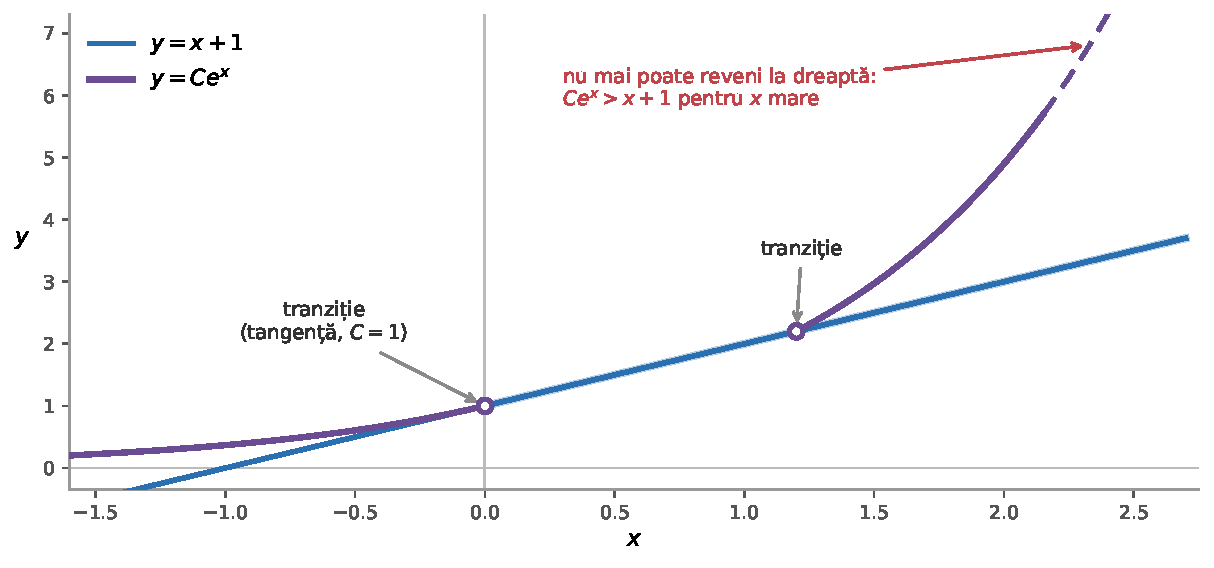
\includegraphics[width=0.86\textwidth]{grafic_p12_nou.pdf}
\caption*{\small\textit{O funcție pe bucăți candidat: alternează între $y=x+1$ (albastru) și $Ce^x$ (mov). Săgețile arată punctele de tranziție. Cheia: odată ce exponențiala depășește dreapta, nu mai poate reveni la ea, deoarece $Ce^x > x+1$ pentru $x$ suficient de mare.}}
\end{figure}

\noindent\textbf{De ce nu funcționează alternarea?} La o tranziție de la exponențial $\to$ liniar trebuie ca $Ce^{x_1} = x_1+1$ și $Ce^{x_1}=1$ (lipire $C^1$), adică tocmai tangența $e^{x_1}\ge x_1+1$, cu egalitate. Singura soluție: $C=1$, $x_1=0$. Dar pentru $x>0$, $e^x > x+1$ strict, deci exponențiala nu mai coboară niciodată la dreaptă. Orice tranziție după $x=0$ este imposibilă. Rămân doar: familia $Ce^x$ (cu $C\ge1$, ca să fie mereu $\ge x+1$) și soluția lipită o singură dată în $x=0$.

\medskip

\emph{Trecerea 2 (redactarea).} Fie $U=\{x:\ f'(x)<x+1\}$ --- mulțime \emph{deschisă}, fiindcă $f'$ e \textbf{continuă} (aici se folosește ipoteza!).

\emph{Pe $U$:} $f(x)=\max(f'(x),x+1)=x+1$, deci, $U$ fiind deschisă, $f'(x)=1$ pe $U$. Dar atunci condiția de apartenență $f'(x)<x+1$ devine $1<x+1$, adică $x>0$: așadar $U\subseteq(0,\infty)$.

\emph{Cazul $U=\varnothing$:} atunci $f'(x)\ge x+1$ peste tot, deci $f(x)=f'(x)$ pentru orice $x$. Ecuația $f'=f$ dă $f(x)=Ce^x$ (prin funcția auxiliară $f(x)e^{-x}$, ca în secțiunea de ecuații diferențiale). Rămâne constrângerea $Ce^x\ge x+1$ pentru orice $x$: pentru $C\le0$ pică în $x=0$; pentru $C>0$, minimul funcției $Ce^x-x-1$ se atinge în $x=-\ln C$ și valorează $\ln C$, deci constrângerea e echivalentă cu $C\ge1$. Obținem familia $f(x)=Ce^x$, $C\ge1$.

\emph{Cazul $U\neq\varnothing$:} fie $(a,b)$ o componentă a lui $U$, cu $0\le a<b\le\infty$. Pe $(a,b)$, $f'\equiv1$; prin continuitatea lui $f'$, $f'(a)=1$. Dar $a\notin U$, deci $f'(a)\ge a+1$, adică $1\ge a+1$, deci $a\le0$: combinat cu $a\ge0$, rezultă $a=0$. Dacă $b<\infty$: la fel $f'(b)=1\ge b+1$, deci $b\le0$ --- contradicție cu $b>0$. Așadar $U=(0,\infty)$, și $f(x)=x+1$ pe $[0,\infty)$ (cu $f(0)=1$ din continuitate). Pe $(-\infty,0]$, complementara lui $U$, avem $f=f'$ (ca mai sus), deci $f(x)=Ce^x$ acolo; $f(0)=1$ dă $C=1$. Verificări finale: lipirea e de clasă $C^1$ ($f'(0-)=e^0=1=f'(0+)$), iar pe $(-\infty,0)$ constrângerea $f'(x)=e^x\ge x+1$ e clasică. \hfill$\blacksquare$

\textbf{Răspuns:} $f(x)=Ce^x$ cu $C\ge1$, \emph{sau} $f(x)=\begin{cases}e^x,&x\le0\\ x+1,&x\ge0.\end{cases}$

\emph{Ce a cumpărat redactarea:} desenul a \emph{ghicit} ambele familii, dar numai argumentul cu mulțimea deschisă $U$ demonstrează că \textbf{nu există altele} --- exact partea invizibilă pe grafic. De remarcat și dicționarul la lucru: „tangenta lui $e^x$ la dreaptă'' $\to$ minimul lui $Ce^x-x-1$ calculat cu derivata; „lipirea merge'' $\to$ verificarea explicită $C^1$; „de la $0$ încolo doar dreapta'' $\to$ argumentul cu capetele componentelor lui $U$.

\subsection{Capcane frecvente (clasa a XI-a)}
\begin{enumerate}[leftmargin=*, itemsep=2pt]
\item Trecerea la limită în recurență cere \emph{mai întâi} demonstrarea convergenței; $\ell=f(\ell)$ singură nu dovedește nimic.
\item Lagrange/Rolle cer continuitate pe intervalul \emph{închis} și derivabilitate pe cel \emph{deschis} --- de verificat explicit ipotezele.
\item Consecințele lui Lagrange (monotonie din semnul derivatei) sunt valabile doar pe \emph{intervale}, nu pe reuniuni de intervale (ex. $-1/x$ are derivată pozitivă pe $\mathbb{R}^*$ dar nu e crescătoare pe $\mathbb{R}^*$).
\item L'Hôpital: de verificat forma nedeterminată și existența limitei raportului derivatelor; implicația nu se inversează.
\item Darboux nu implică continuitate; continuitate implică Darboux.
\item $a_{n+1}-a_n\to 0$ nu implică convergența; $\frac{a_{n+1}}{a_n}\to 1$ nu decide nimic.
\item Punctele de extrem pot fi și în capetele domeniului sau în puncte de nederivabilitate --- Fermat acoperă doar punctele interioare cu derivată.
\item La limite cu $\limsup/\liminf$ sau subșiruri: convergența pe $(x_{2n})$ și $(x_{2n+1})$ trebuie să dea \emph{aceeași} limită.
\end{enumerate}

\subsection{Capcane la integrale (clasa a XII-a)}
\begin{enumerate}[leftmargin=*, itemsep=2pt]
\item „Continuă $\iff$ are primitive'' e fals în ambele rafinări: continuitatea e suficientă dar nu necesară; Darboux e necesară dar nu suficientă.
\item Leibniz--Newton cere ca $G$ să fie primitivă pe \emph{tot} intervalul --- atenție la primitive „pe bucăți'' cu constante nepotrivite la lipire (clasic la $\int\frac{dx}{2+\cos x}$ cu substituția $t=\operatorname{tg}\frac x2$, discontinuă în $\pi$).
\item La schimbarea de variabilă pentru integrale definite se schimbă și capetele; $u$ trebuie să fie derivabilă cu derivata continuă pe intervalul de integrare.
\item $\int_a^b f=0$ nu implică $f\equiv0$ fără ipotezele $f\ge0$ \emph{și} $f$ continuă.
\item Integrabilitatea Riemann cere mărginire; $\int_0^1\frac{dx}{\sqrt x}$ este integrală \emph{improprie}, nu Riemann obișnuită --- se tratează prin limită.
\item În sume Riemann, funcția trebuie să fie integrabilă pe intervalul închis; singularitățile la capete (ca la $x^{-\alpha}$) cer argument suplimentar de trunchiere.
\end{enumerate}

\section{Construcții: ce funcții să încerci}

\emph{Notă:} secțiunea stă la început fiindcă e o \emph{atitudine}, nu un capitol --- se folosește peste tot. Exemplele ei invocă noțiuni tratate riguros mai târziu (derivate, ecuații diferențiale, lipiri pe $\mathbb{Q}$, integrale improprii); la prima citire se pot sări demonstrațiile, reținând reflexele.

Problemele de construcții la ONM sunt, de multe ori, de tipul \emph{„demonstrați că există o funcție cu proprietățile...''} sau \emph{„dați un exemplu de funcție care...''}. Ideea principală: să recunoști rapid \textbf{ce formă de funcție are șanse mari să funcționeze}, apoi să determini parametrii prin calcul direct.

\subsection{Principii generale de construcție}

Problemele de construcție arată la fel în toate ramurile --- combinatorică, teoria numerelor, analiză --- și au un folclor comun de strategii (adaptat aici după materialul „Olympiad Constructions'' al lui Cody Johnson și literatura de combinatorică olimpică):

\begin{enumerate}[leftmargin=*, itemsep=2pt]
\item \textbf{Cazuri mici, întotdeauna primele.} Rezolvă problema pentru $n=1,2,3,4$: cazurile mici îți ghicesc răspunsul (minimul/maximul, forma) și, mai important, îți arată \emph{tiparul} după care se asamblează construcția generală. Echivalentul în analiză: încearcă întâi pe exemplele-jucărie din catalog.
\item \textbf{Construcție prin inducție/asamblare.} Dintr-o construcție de mărime $n$ se fabrică des una de mărime $n+1$ sau $2n$ (dublezi, lipești, adaugi o piesă). În analiză: lipirea funcțiilor pe bucăți ($e^x$ cu $x+1$ la ONM 1994), șirurile de funcții definite recursiv.
\item \textbf{Întâi demonstrează, apoi caută: îngustarea prin restricții.} Înainte de a căuta orbește, demonstrează \emph{proprietăți obligatorii} ale oricărei soluții (în analiză: semne, monotonii, valori forțate în puncte). Fiecare restricție taie din spațiul de căutare --- și de multe ori restricțiile, cumulate, \emph{dictează} construcția. E exact „structura ghicește'' din secțiunile noastre: la $(f')^2+1=f$, compararea gradelor a decis totul înainte de orice încercare.
\item \textbf{La „demonstrați sau infirmați'': atacă serios varianta NU.} Încearcă cu adevărat să demonstrezi imposibilitatea; \emph{locul precis unde argumentul tău eșuează} e harta către construcție --- acolo e libertatea pe care o construcție trebuie s-o exploateze. Și disciplina de concurs: dacă în prima jumătate a timpului n-ai demonstrat „da'', petrece a doua jumătate pe „nu'' --- fără să oscilezi.
\item \textbf{Principiul simplității.} Dacă există o construcție, aproape sigur există una din \emph{piese simple}: mișcări elementare, blocuri repetate, funcții din catalog. Nu căuta obiecte exotice înainte de a epuiza combinațiile banale --- morala tuturor exemplelor din fișă, unde răspunsurile au fost $e^x$, $|x|$, Dirichlet, $\sqrt{x^2+\varepsilon}$, niciodată ceva nemaivăzut.
\end{enumerate}

Restul secțiunii aplică aceste principii la specificul analizei: ce \emph{familii de funcții} joacă rolul „pieselor simple''.

\begin{tehbox}{Reflexul 1: la ecuații funcționale sau diferențiale, încearcă întâi un polinom}

Primul reflex este să presupui că funcția e polinom și să vezi \emph{ce grad ar trebui să aibă}: compararea gradelor spune foarte repede dacă există vreo șansă. Regulile de grad: derivarea scade gradul cu $1$; ridicarea la pătrat îl dublează; compunerea le înmulțește.

\textbf{Exemplu.} Să se construiască $f$ cu $\big(f'(x)\big)^2+1=f(x)$ pentru orice $x$.

\emph{Pasul 1 (gradul).} Dacă $f$ e polinom de grad $n$: $f'$ are grad $n-1$, deci $(f')^2$ are grad $2(n-1)$. Egalitatea gradelor cere $2(n-1)=n$, adică $n=2$. Încercăm $f(x)=ax^2+bx+c$.

\emph{Pasul 2 (calcul direct).} $f'(x)=2ax+b$, deci
\[
(2ax+b)^2+1=ax^2+bx+c
\quad\Longleftrightarrow\quad
4a^2x^2+4abx+b^2+1=ax^2+bx+c,
\]
și identificarea coeficienților dă sistemul $4a^2=a$, $4ab=b$, $b^2+1=c$.

\emph{Pasul 3 (rezolvarea).} Din prima: $a=0$ (pierde gradul 2) sau $a=\frac14$. Pentru $a=\frac14$, a doua ecuație devine $b\cdot0=0$, deci $b$ e \emph{arbitrar}, iar $c=b^2+1$:
\[
\boxed{\ f(x)=\frac{x^2}{4}+bx+b^2+1,\qquad b\in\mathbb{R}.\ }
\]
Verificare: $f'(x)=\frac x2+b$, $\big(\frac x2+b\big)^2+1=\frac{x^2}4+bx+b^2+1=f(x)$. \checkmark

\end{tehbox}

\subsection{Reflexul 2: condiția $f>0$ pe tot domeniul}

Când enunțul cere $f(x)>0$ pentru orice $x$ din domeniu (de obicei $(0,\infty)$), formele naturale de testat sunt
\[
f(x)=c_2\,x^{c_1}\qquad\text{și}\qquad f(x)=b\cdot a^{x},
\]
cu $c_2,b>0$ --- puterile și exponențialele sunt pozitivele „canonice'' și se comportă perfect la înmulțiri, compuneri și derivări (rămân în aceeași familie). Nu întâmplător: acestea sunt exact soluțiile ecuațiilor funcționale clasice (secțiunea de ecuații Cauchy), deci orice condiție cu structură multiplicativă le va selecta.

\subsection{Reflexul 3: discontinuități controlate --- funcții de tip Dirichlet}

Când trebuie construită o funcție cu un număr \emph{controlat} de puncte de discontinuitate sau de nederivabilitate, ideea standard este definirea diferită pe $\mathbb{Q}$ și pe $\mathbb{R}\setminus\mathbb{Q}$. Instrumentul teoretic e deja în fișă (subsecțiunea „Funcții definite prin cazuri pe $\mathbb{Q}$ și $\mathbb{R}\setminus\mathbb{Q}$''): pentru $g,h$ continue, funcția lipită e \textbf{continuă exact în punctele unde $g(x)=h(x)$}, și derivabilă exact unde ramurile se ating cu tot cu derivate. Construcția devine astfel o \emph{ecuație}: vrei discontinuitate exact pe o mulțime $S$? Alege ramuri care coincid exact pe complementara lui $S$.

\subsection{Reflexul 4: Ce funcții clasice care verifică ipoteza știu?}

Înainte de a inventa ceva complicat, pune-ți întrebarea: \emph{„ce exemplu cu proprietățile acestea știu deja?''} Subpunctele de tip „dați un exemplu / rezultă că...?'' de la olimpiadă se rezolvă aproape întotdeauna dintr-un catalog scurt, combinat cu mici ajustări (translații, înmulțiri cu constante, $x^2+\varepsilon$ în loc de $x^2$):

\begin{enumerate}[leftmargin=*, itemsep=2pt]
\item \textbf{Dirichlet} $\mathbf{1}_{\mathbb{Q}}$ --- discontinuă peste tot; $x\cdot\mathbf{1}_{\mathbb{Q}}$ --- continuă doar în $0$; $x$ pe $\mathbb{Q}$, $x+1$ în rest --- discontinuă peste tot dar cu limite „pe ramuri''.
\item $|x|$ --- continuă, nederivabilă într-un punct; $\sqrt{x^2+\varepsilon}$ --- neteda care o aproximează.
\item $\sin\frac1x$ --- mărginită fără limită în $0$; $x\sin\frac1x$ --- continuă, nederivabilă în $0$; $x^2\sin\frac1x$ --- derivabilă cu derivata discontinuă.
\item $x^3$ --- strict crescătoare cu derivata nulă într-un punct; $x+2\sin x$ --- derivată care schimbă semnul de infinite ori, dar funcția $\to\infty$.
\end{enumerate}

Morala: la punctele b) de tip „rezultă că...?'', răspunsul „nu'' se demonstrează cu un membru al catalogului, ajustat minimal.

\subsection*{Exemplu}

\emph{Fie $f:\mathbb{R}\to\mathbb{R}$ pentru care există o funcție derivabilă $g:\mathbb{R}\to\mathbb{R}$ și un șir $(a_n)$ de numere strict pozitive, convergent la $0$, astfel încât}
\[
g'(x)=\lim_{n\to\infty}\frac{f(x+a_n)-f(x)}{a_n}\qquad\forall x\in\mathbb{R}.
\]
\emph{a) Dați un exemplu de astfel de $f$ care nu e derivabilă în niciun punct.}

\emph{Soluție.} Gândim simplu: ne trebuie o funcție nederivabilă peste tot --- primul candidat din catalog e Dirichlet, $f=\mathbf{1}_{\mathbb{Q}}$. Verificăm că merge cu $a_n=\frac1n$: dacă $x\in\mathbb{Q}$, atunci $x+\frac1n\in\mathbb{Q}$; dacă $x\notin\mathbb{Q}$, atunci $x+\frac1n\notin\mathbb{Q}$ --- adunarea unui rațional \emph{păstrează clasa}. Deci
\[
f\Big(x+\frac1n\Big)=f(x)\quad\forall x,n
\qquad\Longrightarrow\qquad
\frac{f(x+a_n)-f(x)}{a_n}=0\to0,
\]
așa că ipoteza e satisfăcută cu $g$ constantă ($g'\equiv0$). Iar $f$ e discontinuă în orice punct (ramurile constante $1$ și $0$ nu se ating nicăieri --- corolarul lipirii), deci nederivabilă peste tot. $\blacksquare$

\emph{De reținut:} toată soluția stă în alegerea șirului $a_n$ \emph{rațional} --- limita pe un șir particular nu vede structura fină a funcției. Exact acest fenomen face ca punctul b) al problemei (dacă $f$ e \emph{continuă}, atunci e derivabilă) să fie partea grea.

\subsection*{Exemplu: ONM 2026, etapa națională, clasa a XI-a, Problema 1b)}

\textbf{Enunț.} Fie $h:\mathbb{R}\to\mathbb{R}$ o funcție continuă și $(f_n)$, $(g_n)$ două șiruri de funcții derivabile cu proprietatea că $f_n(x)<h(x)<g_n(x)$ pentru orice $x\in\mathbb{R}$ și orice $n\in\mathbb{N}^*$, și că $g_n(x)-f_n(x)\to0$ pentru orice $x\in\mathbb{R}$. Este $h$ neapărat derivabilă?

\textbf{Răspuns: NU.}

Am participat la ONM 2026 și acesta a fost raționamentul meu la această problemă.

\emph{Cum se ghicește contraexemplul.} În timpul concursului am desenat un grafic. Condițiile problemei spun că $h$ e prinsă între două familii de funcții derivabile care o strivesc --- pe grafic asta înseamnă două „clești'' de curbe netede care coboară și urcă spre $h$ din ambele părți. Singura funcție continuă și nederivabilă pe care o știam era $h(x)=|x|$ --- are un colț în $0$, dar e altfel perfect inofensivă. Am desenat-o și am căutat cu ochii niște curbe derivabile, mai sus și mai jos, care să o strângă:

\begin{center}
\begin{tikzpicture}[scale=2.0, >=latex]
  % Axe
  \draw[->] (-1.30,0) -- (1.32,0) node[right] {$x$};
  \draw[->] (0,-0.50) -- (0,1.28) node[above] {$y$};
  \node[below left, font=\small] at (0,0) {$0$};

  % Curbe de sus -- violet, intrerupte
  \draw[onm!35, line width=0.85pt, dashed, domain=-1.28:1.28, samples=100]
    plot (\x, {sqrt(\x*\x + 1)});
  \draw[onm!65, line width=1pt, dashed, domain=-1.28:1.28, samples=100]
    plot (\x, {sqrt(\x*\x + 0.25)});
  \draw[onm, line width=1.3pt, dashed, domain=-1.28:1.28, samples=100]
    plot (\x, {sqrt(\x*\x + 0.04)});

  % Curbe de jos -- portocaliu, punctate, coboara sub 0
  \draw[ojm!35, line width=0.85pt, dotted, domain=-1.28:1.28, samples=100]
    plot (\x, {sqrt(\x*\x + 1) - 1.4142});
  \draw[ojm!65, line width=1pt, dotted, domain=-1.28:1.28, samples=100]
    plot (\x, {sqrt(\x*\x + 0.25) - 0.7071});
  \draw[ojm, line width=1.3pt, dotted, domain=-1.28:1.28, samples=100]
    plot (\x, {sqrt(\x*\x + 0.04) - 0.2828});

  % |x| -- linie groasa, desenata dupa curbe ca sa fie deasupra
  \draw[ink, line width=2.4pt, domain=-1.28:0, samples=2]
    plot (\x, {-\x});
  \draw[ink, line width=2.4pt, domain=0:1.28, samples=2]
    plot (\x, {\x});

  % Eticheta h(x) -- in interiorul graficului, la stanga
  \node[ink, font=\small\bfseries, fill=white, inner sep=1pt]
    at (-0.75, 0.88) {$h(x)=|x|$};

  % Punct de colt
  \filldraw[ink] (0,0) circle (0.030);
  \node[ink, above right, font=\small] at (0.05, 0.04) {colț};

  % Etichete sus/jos
  \node[onm, font=\scriptsize\itshape] at (0.60, 1.15) {sus};
  \node[ojm, font=\scriptsize\itshape] at (0.75, 0.55) {jos};
\end{tikzpicture}
\end{center}

Forma curbelor de deasupra mi-a sugerat imediat o hiperbolă netezită. Odată ales $h$ și observat că curbele seamănă cu $\sqrt{x^2+\varepsilon}$, am ales formal:

\textbf{Construcția.} Punem
\[
g_n(x)=\sqrt{x^2+\tfrac1n},\qquad f_n(x)=\sqrt{x^2+\tfrac1n}-\sqrt{\tfrac2n}.
\]
\emph{Derivabilitate:} $x^2+\frac1n>0$, deci ambele sunt $C^\infty$ pe $\mathbb{R}$.

\emph{Încadrarea $f_n<h<g_n$:} Inegalitatea $g_n>|x|$ e clară. Inegalitatea $f_n<|x|$ revine la $\sqrt{x^2+\frac1n}-\sqrt{\frac2n}<|x|$, adică (ridicând la pătrat, ambii membri nenegativi pentru $n$ mare):
\[
x^2+\frac1n < x^2+2|x|\sqrt{\tfrac2n}+\frac2n
\quad\Longleftrightarrow\quad
0 < 2|x|\sqrt{\tfrac2n}+\frac1n,
\]
adevărată pentru orice $x\in\mathbb{R}$.

\emph{Strângerea:} $g_n(x)-f_n(x)=\sqrt{\frac2n}\to0$ uniform.

Toate ipotezele sunt satisfăcute, dar $h=|x|$ nu e derivabilă în $0$. $\blacksquare$



\chapter{Clasa a XI-a}
\section{Topologie pe $\mathbb{R}$}

\emph{Notă:} secțiunea folosește limite de șiruri, criteriul lui Heine și continuitatea --- noțiuni de clasă, tratate riguros în secțiunile următoare; le folosim aici în accepțiunea standard.

\subsection{Mulțimi dense}

\begin{definitie}
O mulțime $A\subseteq\mathbb{R}$ este \textbf{densă} în $\mathbb{R}$ dacă orice interval deschis nedegenerat conține puncte din $A$. Echivalent (prin alegerea de puncte în intervalele $\big(x-\frac1n,x+\frac1n\big)$): orice număr real e limita unui șir de elemente din $A$.
\end{definitie}

\begin{teorema}[Densitatea lui $\mathbb{Q}$ și a lui $\mathbb{R}\setminus\mathbb{Q}$]
$\mathbb{Q}$ și $\mathbb{R}\setminus\mathbb{Q}$ sunt dense în $\mathbb{R}$.
\end{teorema}
\begin{proof}
Fie $a<b$. Alegem $n\in\mathbb{N}^*$ cu $n>\frac{1}{b-a}$ (proprietatea lui Arhimede), deci $\frac1n<b-a$: pasul $\frac1n$ nu poate „sări'' peste intervalul $(a,b)$. Formal, $k=\lfloor na\rfloor+1$ dă $na<k\le na+1<nb$, deci $\frac kn\in(a,b)$ --- un rațional. Pentru iraționale: intervalul $(a-\sqrt2,\,b-\sqrt2)$ conține un rațional $q$, deci $q+\sqrt2\in(a,b)$ e irațional (rațional $+$ irațional $=$ irațional).
\end{proof}

\begin{teorema}[Principiul densității]
Fie $A$ densă în $\mathbb{R}$ și $f,g:\mathbb{R}\to\mathbb{R}$ \emph{continue} cu $f(x)=g(x)$ pentru orice $x\in A$. Atunci $f=g$ pe tot $\mathbb{R}$.
\end{teorema}
\begin{proof}
Fie $x\in\mathbb{R}$ și un șir $(a_n)\subset A$ cu $a_n\to x$ (densitate). Prin Heine și continuitate: $f(x)=\lim f(a_n)=\lim g(a_n)=g(x)$.
\end{proof}

\begin{obs}
Acesta e mecanismul din spatele multor probleme de rigiditate: informația despre $f$ pe o mulțime densă (de pildă $\mathbb{Q}$) plus continuitatea determină $f$ complet --- exact pașii finali din ecuațiile funcționale de tip Cauchy (secțiunea de continuitate). Un exemplu important de mulțime densă, dincolo de $\mathbb{Q}$: complementara oricărei mulțimi cel mult numărabile --- vezi subsecțiunea următoare.
\end{obs}

\subsection{Mulțimi numărabile}

\begin{definitie}
O mulțime $A$ este \textbf{numărabilă} dacă elementele ei pot fi \emph{înșirate} într-un șir: $A=\{a_1,a_2,a_3,\dots\}$, fiecare element apărând (cel puțin o dată) pe listă. $A$ este \textbf{cel mult numărabilă} dacă e finită sau numărabilă. Intuiția: „numărabil'' $=$ poți face inventarul complet, element cu element, chiar dacă inventarul nu se termină niciodată.
\end{definitie}

\begin{propozitie}[$\mathbb{Z}$ și $\mathbb{Q}$ sunt numărabile]
\emph{$\mathbb{Z}$:} se înșiră prin alternare, $0,\,1,\,-1,\,2,\,-2,\,3,\,-3,\dots$ --- fiecare întreg apare exact o dată.

\emph{$\mathbb{Q}$:} scriem fiecare rațional ca $\frac pq$ cu $q\ge1$ și grupăm fracțiile după „mărimea'' $|p|+q$: grupa $1$ conține $\frac01$; grupa $2$: $\frac11,\frac{-1}{1}$; grupa $3$: $\frac21,\frac{-2}{1},\frac12,\frac{-1}{2}$; și așa mai departe. Fiecare grupă e \emph{finită} (pentru $|p|+q=n$ sunt cel mult $2n$ fracții), iar orice rațional cade într-o grupă --- deci listarea grupă după grupă înșiră tot $\mathbb{Q}$. Numerele care apar de mai multe ori (ex.\ $\frac12=\frac24$) se păstrează doar la prima apariție.
\end{propozitie}

\begin{obs}[Reguli de calcul cu numărabilitatea]
(1) O submulțime a unei mulțimi cel mult numărabile e cel mult numărabilă (din lista mare ștergi ce nu-ți trebuie). (2) Reuniunea a două --- și chiar a unui șir de --- mulțimi cel mult numărabile e cel mult numărabilă: listele se împletesc, exact ca la $\mathbb{Z}$ sau ca gruparea de la $\mathbb{Q}$. (3) De aceea, la teorema despre discontinuitățile funcțiilor monotone (secțiunea de continuitate), injecția în $\mathbb{Q}$ încheie demonstrația: o mulțime care se scufundă în $\mathbb{Q}$ e cel mult numărabilă.
\end{obs}

\begin{lema}[Intervalele nu sunt numărabile; densitatea complementarei]
Un interval nedegenerat nu este cel mult numărabil. În consecință, complementara unei mulțimi cel mult numărabile intersectează orice interval nedegenerat --- adică este \textbf{densă} în $\mathbb{R}$.
\end{lema}
\begin{proof}
Fie $(a_n)_{n\ge1}$ un șir oarecare de numere reale și $(\alpha,\beta)$ un interval nedegenerat; arătăm că în $(\alpha,\beta)$ există un punct care nu apare în șir. Construim inductiv intervale închise nedegenerate $I_1\supseteq I_2\supseteq\dots$, cu $I_1\subset(\alpha,\beta)$ și $a_n\notin I_n$: împărțim la fiecare pas intervalul curent în trei subintervale închise egale și alegem unul care nu-l conține pe $a_{n+1}$ (punctul $a_{n+1}$ nu poate atinge toate trei). Cu $I_n=[p_n,q_n]$: șirul $(p_n)$ e crescător și majorat de $q_1$, deci convergent la un $x$; din $p_n\le q_m$ pentru orice $n,m$ rezultă $p_m\le x\le q_m$, adică $x\in I_m$ pentru orice $m$. Deci $x\neq a_m$ pentru toți $m$ și $x\in(\alpha,\beta)$: niciun șir nu poate epuiza intervalul. Consecința: dacă $N$ e cel mult numărabilă, $N$ nu poate conține un interval nedegenerat, deci orice astfel de interval conține puncte din afara lui $N$.
\end{proof}

\begin{obs}[Densă vs.\ numărabilă: două „mărimi'' diferite]
$\mathbb{Q}$ este simultan \emph{densă} (are puncte în orice interval --- e „peste tot'') și \emph{numărabilă} (încape într-o listă --- e „mică''), în timp ce $\mathbb{R}\setminus\mathbb{Q}$ e densă și \emph{ne}numărabilă (altfel $\mathbb{R}=\mathbb{Q}\cup(\mathbb{R}\setminus\mathbb{Q})$ ar fi numărabil, contrazicând lema). Cele două noțiuni măsoară lucruri complet diferite: unde stau punctele, respectiv câte sunt. Perechea dens $+$ numărabil revine constant în fișă: la discontinuitățile funcțiilor monotone și la problema OJM 2024 (secțiunea de continuitate), și --- sub numele de „mulțime neglijabilă'' --- la criteriul lui Lebesgue (Partea a III-a), unde $\mathbb{Q}$ se dovedește nu doar numărabilă, ci și „fără grosime''.
\end{obs}

\subsection{Teorema lui Kronecker}

Pentru $x\in\mathbb{R}$ notăm $\{x\}=x-\lfloor x\rfloor\in[0,1)$ \emph{partea fracționară}.

\begin{teorema}[Kronecker]
Fie $\alpha\in\mathbb{R}\setminus\mathbb{Q}$. Atunci mulțimea $\big\{\{n\alpha\}:n\in\mathbb{N}^*\big\}$ este densă în $[0,1]$. Echivalent: mulțimea $\{m+n\alpha:\ m\in\mathbb{Z},\ n\in\mathbb{N}^*\}$ este densă în $\mathbb{R}$.
\end{teorema}
\begin{proof}
\emph{Pasul 1 (cutia lui Dirichlet).} Fie $N\in\mathbb{N}^*$. Împărțim $[0,1)$ în $N$ intervale de lungime $\frac1N$. Cele $N+1$ numere $\{0\cdot\alpha\},\{1\cdot\alpha\},\dots,\{N\alpha\}$ nu încap în $N$ cutii fără ca două să pice în aceeași: există $0\le p<q\le N$ cu
\[
\big|\{q\alpha\}-\{p\alpha\}\big|<\frac1N.
\]
Fie $r=q-p\in\{1,\dots,N\}$. Numărul $\{q\alpha\}-\{p\alpha\}=r\alpha-\big(\lfloor q\alpha\rfloor-\lfloor p\alpha\rfloor\big)$ diferă de $r\alpha$ printr-un întreg, deci $\beta:=\{r\alpha\}$ satisface $\beta<\frac1N$ sau $\beta>1-\frac1N$; în ambele cazuri, „pasul'' $\beta$ este la distanță $<\frac1N$ de un întreg, dar \emph{nu este} întreg ($\alpha$ irațional $\Rightarrow$ $r\alpha\notin\mathbb{Z}$).

\emph{Pasul 2 (pași mici umplu intervalul).} Considerăm șirul $\{r\alpha\}$, $\{2r\alpha\}$, $\{3r\alpha\}$, \dots{} Fiecare termen se obține din precedentul adunând $\beta$ și, eventual, scăzând $1$ (la „înfășurare''): pașii consecutivi au lungimea $\min(\beta,1-\beta)<\frac1N$. Un șir care pornește din $[0,1)$ și avansează cu pași de lungime $<\frac1N$, fără să se oprească (termenii sunt distincți: $\{i r\alpha\}=\{j r\alpha\}$ ar face $(i-j)r\alpha\in\mathbb{Z}$, imposibil), vizitează orice subinterval al lui $[0,1)$ de lungime $\frac1N$: nu poate „sări'' peste el. Deci orice interval $\big(c-\frac1{2N},c+\frac1{2N}\big)\subseteq[0,1)$ conține un $\{n\alpha\}$. Cum $N$ era arbitrar, mulțimea e densă.
\end{proof}

\begin{obs}[Aplicații tipice]
(1) $\{\sin n:\ n\in\mathbb{N}\}$ e densă în $[-1,1]$ (se scrie $n=2\pi\cdot\frac{n}{2\pi}$ și se folosește Kronecker pentru $\alpha=\frac{1}{2\pi}$, apoi continuitatea lui $\sin$ pe cercul unitate) --- în particular șirul $(\sin n)$ \emph{nu are limită}. (2) Problemele de tip „arătați că există $n$ cu primele cifre ale lui $2^n$ egale cu...'' se reduc la densitatea lui $\{n\lg2\}$, cu $\lg2$ irațional.
\end{obs}

\subsection{Funcții periodice și mulțimea perioadelor}

\begin{propozitie}
Fie $f:\mathbb{R}\to\mathbb{R}$ continuă și periodică (există $T>0$ cu $f(x+T)=f(x)$).
\begin{enumerate}[leftmargin=*, itemsep=1pt]
\item Dacă $f$ este neconstantă, atunci $f$ are o \textbf{cea mai mică perioadă} strict pozitivă.
\item Dacă $f$ are limită finită la $+\infty$, atunci $f$ este constantă.
\item Dacă $f$ admite două perioade $T_1,T_2>0$ cu raportul $T_1/T_2$ \emph{irațional}, atunci $f$ este constantă.
\end{enumerate}
\end{propozitie}
\begin{proof}
Observația de bază: mulțimea perioadelor (împreună cu $0$ și opusele) este închisă la sume și diferențe; iar dacă $f$ e continuă și are un șir de perioade $t_n\to0$, $t_n\neq 0$, atunci $f$ e constantă --- pentru orice $x$, numerele $\{k\,t_n:k\in\mathbb{Z}\}$ formează, când $n$ crește, o rețea tot mai fină, deci $x$ e limită de puncte de forma $k\,t_n$, unde $f$ ia valoarea $f(0)$; continuitatea dă $f(x)=f(0)$.

\emph{1.} Fie $T_0\ge0$ infimumul perioadelor strict pozitive. Dacă $T_0=0$, există perioade oricât de mici și, prin cele de mai sus, $f$ e constantă, contradicție. Deci $T_0>0$. Dacă $T_0$ nu ar fi perioadă, ar exista perioade $T>T'$ în intervalul $(T_0,\,T_0+\varepsilon)$, pentru orice $\varepsilon>0$ (altfel intervalul ar conține cel mult o perioadă, iar $T_0$ n-ar mai fi infimum); atunci $T-T'$ e o perioadă cu $0<T-T'<\varepsilon$. Luând $\varepsilon<T_0$ obținem o perioadă mai mică decât $T_0$, contradicție. Așadar $T_0$ e perioadă și este cea mai mică perioadă strict pozitivă.
\emph{2.} Pentru $x$ fixat, $f(x)=f(x+nT)\to\lim_{y\to\infty}f(y)=\ell$, deci $f\equiv\ell$.
\emph{3.} Numerele $mT_1+nT_2$ ($m,n\in\mathbb{Z}$) sunt toate perioade (sau $0$); prin Kronecker aplicat lui $\alpha=T_1/T_2\notin\mathbb{Q}$, mulțimea $\{mT_1+nT_2\}$ e densă în $\mathbb{R}$, în particular conține perioade oricât de mici --- deci $f$ e constantă.
\end{proof}

\begin{obs}
Punctul 3 e aplicația-vedetă a lui Kronecker la funcții: de pildă, o funcție continuă cu $f(x+1)=f(x)$ și $f(x+\sqrt2)=f(x)$ e neapărat constantă. Fără continuitate, afirmația pică (există exemple „sălbatice'').
\end{obs}


\section{Șiruri de numere reale}

\subsection{Definiții fundamentale și mărginire}

\begin{definitie}
Șirul $(a_n)_{n\ge 1}$ are limita $\ell\in\mathbb{R}$ dacă
$\forall\, \varepsilon>0,\ \exists\, N\in\mathbb{N}$ astfel încât $|a_n-\ell|<\varepsilon$ pentru orice $n\ge N$. Șirul are limita $+\infty$ dacă $\forall\, M>0,\ \exists\, N$ cu $a_n>M$ pentru $n\ge N$ (analog $-\infty$).
\end{definitie}

\begin{teorema}[Unicitatea limitei; mărginirea șirurilor convergente]
Limita unui șir, dacă există, este unică. Orice șir convergent este mărginit.
\end{teorema}

\begin{teorema}[Weierstrass]
Orice șir monoton și mărginit este convergent. Mai precis: dacă $(a_n)$ este crescător și mărginit superior, atunci $a_n \to \sup_n a_n$; dacă e crescător și nemărginit, $a_n\to+\infty$.
\end{teorema}

\begin{tehbox}{Schema standard pentru șiruri recurente}
Pentru $x_{n+1}=f(x_n)$ cu $f$ continuă:
\begin{enumerate}[leftmargin=*, itemsep=1pt]
\item Se caută un interval invariant $I$ (adică $f(I)\subseteq I$) care conține $x_1$ --- de obicei prin inducție.
\item Se studiază monotonia: semnul lui $f(x)-x$ pe $I$, sau (dacă $f$ e crescătoare) compararea $x_2$ cu $x_1$.
\item Monoton + mărginit $\Rightarrow$ convergent (Weierstrass). Limita $\ell$ verifică $\ell=f(\ell)$ (trecere la limită în recurență, folosind continuitatea).
\item Dacă $f$ este \emph{descrescătoare}, șirul nu e monoton, dar subșirurile $(x_{2n})$ și $(x_{2n+1})$ sunt monotone (căci $f\circ f$ e crescătoare); se arată că au aceeași limită.
\end{enumerate}
\end{tehbox}

\subsection{Subșiruri, Bolzano--Weierstrass, șiruri Cauchy}

\begin{teorema}
Dacă $a_n\to\ell$, atunci orice subșir $a_{n_k}\to\ell$. Reciproc: dacă $(a_{2n})$ și $(a_{2n+1})$ converg la aceeași limită $\ell$, atunci $a_n\to\ell$.
\end{teorema}

\begin{lema}[Lema lui Cesàro / Bolzano--Weierstrass]
Orice șir mărginit de numere reale conține un subșir convergent.
\end{lema}

\begin{definitie}
$(a_n)$ este \textbf{șir Cauchy (fundamental)} dacă $\forall\varepsilon>0,\ \exists N$ astfel încât $|a_m-a_n|<\varepsilon$ pentru orice $m,n\ge N$.
\end{definitie}

\begin{teorema}[Criteriul lui Cauchy]
Un șir de numere reale este convergent dacă și numai dacă este șir Cauchy.
\end{teorema}

\begin{obs}
Utilizare tipică la olimpiadă: $|a_{n+1}-a_n|\le c\, q^n$ cu $q\in(0,1)$ implică $(a_n)$ Cauchy (prin sumă geometrică telescopică), deci convergent --- fără a cunoaște limita. Atenție: $a_{n+1}-a_n\to 0$ \emph{nu} este suficient (contraexemplu: $a_n=\sqrt{n}$ sau $a_n=H_n=1+\tfrac12+\dots+\tfrac1n$).
\end{obs}

\subsection{Puncte limită; limită superioară și inferioară}

\begin{definitie}
Pentru $(a_n)$ mărginit, $\displaystyle\limsup_{n\to\infty} a_n=\lim_{n\to\infty}\Big(\sup_{k\ge n} a_k\Big)$ și $\displaystyle\liminf_{n\to\infty} a_n=\lim_{n\to\infty}\Big(\inf_{k\ge n} a_k\Big)$; limitele există fiindcă șirul supremumurilor e descrescător și mărginit (respectiv, cel al infimumurilor, crescător). Convenție: pentru un șir nemărginit superior, $\limsup a_n=+\infty$; nemărginit inferior, $\liminf a_n=-\infty$.
\end{definitie}

\begin{propozitie}[Caracterizarea cu $\varepsilon$]
Fie $(a_n)$ mărginit și $L\in\mathbb{R}$. Atunci $L=\limsup a_n$ dacă și numai dacă, pentru orice $\varepsilon>0$:
(i) $a_n<L+\varepsilon$ \emph{de la un rang încolo}; și
(ii) $a_n>L-\varepsilon$ \emph{pentru o infinitate de indici}.
Dual, $\ell=\liminf a_n$ $\iff$ $a_n>\ell-\varepsilon$ de la un rang încolo și $a_n<\ell+\varepsilon$ pentru o infinitate de $n$.
\end{propozitie}
\begin{proof}
Fie $s_n=\sup_{k\ge n}a_k\searrow L_0=\limsup a_n$.
($\Rightarrow$) Dacă $L=L_0$: (i) există $N$ cu $s_N<L+\varepsilon$, deci $a_n\le s_N<L+\varepsilon$ pentru $n\ge N$. (ii) Pentru orice $N$, $s_N\ge L>L-\varepsilon$, deci, din definiția supremumului, există $k\ge N$ cu $a_k>L-\varepsilon$; cum $N$ e arbitrar, astfel de indici sunt o infinitate.
($\Leftarrow$) Din (i): $s_n\le L+\varepsilon$ de la un rang încolo, deci $L_0\le L+\varepsilon$. Din (ii): pentru orice $n$ există $k\ge n$ cu $a_k>L-\varepsilon$, deci $s_n\ge L-\varepsilon$, adică $L_0\ge L-\varepsilon$. Cum $\varepsilon>0$ e arbitrar, $L_0=L$.
\end{proof}

\begin{definitie}
$\ell\in\mathbb{R}$ este \textbf{punct limită} (valoare de aderență) al șirului $(a_n)$ dacă există un subșir $a_{n_k}\to\ell$. Notăm cu $A$ mulțimea punctelor limită.
\end{definitie}

\begin{propozitie}[Structura mulțimii punctelor limită]
Fie $(a_n)$ mărginit, $m=\liminf a_n$, $M=\limsup a_n$. Atunci $A\neq\varnothing$, $A\subseteq[m,M]$, iar $m=\min A$ și $M=\max A$: limsup și liminf sunt \emph{cel mai mare}, respectiv \emph{cel mai mic} punct limită.
\end{propozitie}
\begin{proof}
$A\neq\varnothing$ e Bolzano--Weierstrass. Dacă $a_{n_k}\to\ell$: pentru orice $\varepsilon>0$, de la un rang încolo $a_n<M+\varepsilon$ (caracterizarea cu $\varepsilon$), deci $\ell\le M+\varepsilon$; $\varepsilon$ arbitrar dă $\ell\le M$; analog $\ell\ge m$. Pentru $M\in A$: pentru fiecare $j$, din caracterizare există o infinitate de indici cu $a_n>M-\frac1j$ și, de la un rang încolo, $a_n<M+\frac1j$; alegem deci $n_j>n_{j-1}$ cu $M-\frac1j<a_{n_j}<M+\frac1j$ --- subșirul construit tinde la $M$. Analog $m\in A$.
\end{proof}

\begin{propozitie}
$a_n\to\ell$ $\iff$ $\liminf a_n=\limsup a_n=\ell$.
\end{propozitie}

\begin{teorema}[Criteriul punctului limită unic]
Un șir \textbf{mărginit} este convergent dacă și numai dacă are un \textbf{singur} punct limită; în acest caz limita e unicul punct limită.
\end{teorema}
\begin{proof}
($\Rightarrow$) Orice subșir al unui șir convergent tinde la limită, deci $A=\{\ell\}$.
($\Leftarrow$) Fie $A=\{\ell\}$ și, prin absurd, $a_n\not\to\ell$: există $\varepsilon_0>0$ și un subșir $(a_{n_k})$ cu $|a_{n_k}-\ell|\ge\varepsilon_0$. Acest subșir e mărginit, deci (Bolzano--Weierstrass) conține un sub-subșir convergent la un $\ell'$ cu $|\ell'-\ell|\ge\varepsilon_0$ --- un al doilea punct limită, contradicție.
\end{proof}

\begin{tehbox}{Metoda punctelor limită}
\begin{enumerate}[leftmargin=*, itemsep=1pt]
\item Se verifică \textbf{mărginirea}: atunci $A\neq\varnothing$ și $A\subseteq[-M,M]$.
\item Din relația care definește șirul se deduce o \textbf{proprietate de închidere} a lui $A$: „dacă $\lambda\in A$, atunci $T(\lambda)\in A$'' --- trecând la limită pe subșiruri, exact ca la recurențe.
\item Se arată că proprietatea \textbf{forțează} $A=\{\ell\}$: de pildă, iterarea lui $T$ ar scoate punctele din compactul $[-M,M]$, sau $A$ ar trebui să fie un interval degenerat.
\item Concluzia, din criteriul punctului limită unic.
\end{enumerate}
Avantajul metodei: nu cere nici monotonie, nici formulă explicită.
\end{tehbox}

\textbf{Exemplu.} \emph{Fie $(u_n)_{n\ge1}$ mărginit astfel încât $u_n+\dfrac{u_{2n}}{2}\to1$. Arătați că $(u_n)$ converge și determinați-i limita.}

\emph{Soluție.} Fie $M>0$ cu $|u_n|\le M$; atunci $A\neq\varnothing$ și $A\subseteq[-M,M]$.
\emph{Închiderea:} dacă $\lambda\in A$, cu $u_{n_k}\to\lambda$, din ipoteză $u_{2n_k}=2\big(1-u_{n_k}\big)+\varepsilon_k$ cu $\varepsilon_k\to0$, deci $u_{2n_k}\to2-2\lambda$, iar $(u_{2n_k})$ e subșir al lui $(u_n)$: așadar $T(\lambda)=2-2\lambda\in A$.
\emph{Forțarea:} punctul fix al lui $T$ este $\frac23$, iar $T(\lambda)-\frac23=-2\big(\lambda-\frac23\big)$, deci $T^m(\lambda)-\frac23=(-2)^m\big(\lambda-\frac23\big)$. Dacă ar exista $\lambda_0\in A$, $\lambda_0\neq\frac23$, toate iteratele $T^m(\lambda_0)$ ar fi în $A\subseteq[-M,M]$, dar $|T^m(\lambda_0)|\to\infty$ --- contradicție. Deci $A=\{\frac23\}$ și $u_n\to\dfrac23$. $\blacksquare$

\textbf{Exemplu.} \emph{Fie $(u_n)$ cu $u_{n+1}-u_n\to0$. Atunci mulțimea $A$ a punctelor limită e un interval; în particular, dacă $(u_n)$ e mărginit, $A=[\liminf u_n,\limsup u_n]$.}

\emph{Soluție (cazul mărginit).} Fie $m=\liminf u_n$, $M=\limsup u_n$; știm $A\subseteq[m,M]$ și $m,M\in A$. Fie $\lambda\in(m,M)$; arătăm $\lambda\in A$. Fie $\varepsilon\in\big(0,\min(\lambda-m,M-\lambda)\big)$ și $N$ arbitrar, mărit astfel încât $|u_{n+1}-u_n|<\varepsilon$ pentru $n\ge N$. Din caracterizarea cu $\varepsilon$: $u_n<m+\varepsilon<\lambda$ pentru o infinitate de indici, și $u_n>\lambda$ tot pentru o infinitate. Alegem $p\ge N$ cu $u_p<\lambda$, apoi $q>p$ cu $u_q>\lambda$, și fie
\[
n=\max\{k:\ p\le k<q,\ u_k\le\lambda\}
\]
(mulțime nevidă --- îl conține pe $p$ --- și finită). Din maximalitate $u_{n+1}>\lambda$, deci
\[
\lambda<u_{n+1}<u_n+\varepsilon\le\lambda+\varepsilon
\quad\Longrightarrow\quad
|u_n-\lambda|<\varepsilon,\ \ n\ge N.
\]
Pentru orice $\varepsilon$ și orice rang, șirul revine la distanță $<\varepsilon$ de $\lambda$: construim inductiv un subșir $\to\lambda$, deci $\lambda\in A$. $\blacksquare$

\emph{Corolar util:} mărginit + pași mici + $A$ finită (sau numărabilă) $\Rightarrow$ convergent (un interval cel mult numărabil e degenerat). \emph{Legătura cu recurențele:} dacă în plus $u_{n+1}=f(u_n)$ cu $f$ continuă, orice punct limită e punct fix ($u_{n_k+1}=f(u_{n_k})\to f(\lambda)$, dar și $u_{n_k+1}=u_{n_k}+(u_{n_k+1}-u_{n_k})\to\lambda$).

\begin{teorema}[Inegalitățile fundamentale pentru $\liminf$ și $\limsup$]
Pentru șiruri mărginite $(a_n),(b_n)$:
\[
\begin{aligned}
\liminf a_n+\liminf b_n&\ \le\ \liminf\,(a_n+b_n)\ \le\ \liminf a_n+\limsup b_n\\
&\ \le\ \limsup\,(a_n+b_n)\ \le\ \limsup a_n+\limsup b_n.
\end{aligned}
\]
\end{teorema}
\begin{proof}
Notăm $\alpha=\liminf a_n$, $A=\limsup a_n$, $\beta=\liminf b_n$, $B=\limsup b_n$.

\emph{Extremele.} Fie $\varepsilon>0$: de la un rang încolo $a_n<A+\varepsilon$ și $b_n<B+\varepsilon$ (caracterizarea cu $\varepsilon$), deci $a_n+b_n<A+B+2\varepsilon$, de unde $\limsup(a_n+b_n)\le A+B+2\varepsilon$, apoi $\le A+B$. Analog, cu minorări, $\liminf(a_n+b_n)\ge\alpha+\beta$.

\emph{Mijlocul, partea stângă} ($\liminf(a_n+b_n)\le\alpha+B$): alegem un subșir $a_{n_k}\to\alpha$ (posibil: $\alpha=\min A_{\text{pcte}}$). Șirul $(b_{n_k})$ e mărginit, deci are un sub-subșir $b_{n_{k_j}}\to\beta'$, cu $\beta'\le B$ (punct limită al lui $(b_n)$). Atunci $a_{n_{k_j}}+b_{n_{k_j}}\to\alpha+\beta'$ e punct limită al sumei, deci $\liminf(a_n+b_n)\le\alpha+\beta'\le\alpha+B$.

\emph{Mijlocul, partea dreaptă} ($\alpha+B\le\limsup(a_n+b_n)$): alegem $b_{n_k}\to B$ și extragem $a_{n_{k_j}}\to\alpha'\ge\alpha$; atunci $\alpha'+B$ e punct limită al sumei, deci $\limsup(a_n+b_n)\ge\alpha'+B\ge\alpha+B$.
\end{proof}

\begin{corolar}[Un șir converge $\Rightarrow$ egalitate]
Dacă $a_n\to a$, atunci $\liminf(a_n+b_n)=a+\liminf b_n$ și $\limsup(a_n+b_n)=a+\limsup b_n$. (Aici $\alpha=A=a$ și lanțul se strânge.) Dacă în plus $a>0$ și $b_n\ge0$, la fel pentru produs: $\limsup(a_nb_n)=a\limsup b_n$.
\end{corolar}

\begin{obs}
Extremele pot fi stricte: pentru $a_n=(-1)^n$, $b_n=(-1)^{n+1}$: $\liminf a_n+\liminf b_n=-2<0=\liminf(a_n+b_n)=\limsup(a_n+b_n)<2=\limsup a_n+\limsup b_n$. Greșeala clasică la concurs: „$\limsup(a_n+b_n)=\limsup a_n+\limsup b_n$'' --- adevărată doar cu $\le$, cu egalitate când unul dintre șiruri converge.
\end{obs}

\begin{teorema}[Rădăcină vs.\ raport]
Pentru $a_n>0$:
\[
\liminf\frac{a_{n+1}}{a_n}\ \le\ \liminf\sqrt[n]{a_n}\ \le\ \limsup\sqrt[n]{a_n}\ \le\ \limsup\frac{a_{n+1}}{a_n}.
\]
\end{teorema}
\begin{proof}
Dreapta (stânga e analogă, mijlocul evident): fie $L=\limsup\frac{a_{n+1}}{a_n}<\infty$ (altfel nimic de arătat) și $\varepsilon>0$: există $N$ cu $\frac{a_{n+1}}{a_n}<L+\varepsilon$ pentru $n\ge N$. Telescopic, pentru $n>N$:
\[
a_n=a_N\cdot\frac{a_{N+1}}{a_N}\cdots\frac{a_n}{a_{n-1}}\le C\,(L+\varepsilon)^n,\qquad C=a_N(L+\varepsilon)^{-N},
\]
deci $\sqrt[n]{a_n}\le C^{1/n}(L+\varepsilon)\to L+\varepsilon$, de unde $\limsup\sqrt[n]{a_n}\le L+\varepsilon$, apoi $\le L$.
\end{proof}

\begin{corolar}
Dacă $\frac{a_{n+1}}{a_n}\to\ell$, atunci $\sqrt[n]{a_n}\to\ell$ (criteriul radicalului, acum cu demonstrație). Reciproca e falsă: pentru $a_n=2^{(-1)^n}$, $\sqrt[n]{a_n}\to1$, dar raportul oscilează:
\[
\liminf\frac{a_{n+1}}{a_n}=\frac14\ <\ 1=\lim\sqrt[n]{a_n}\ <\ 4=\limsup\frac{a_{n+1}}{a_n}.
\]
Morala: criteriul rădăcinii e cel puțin la fel de puternic ca al raportului.
\end{corolar}

\subsection{Contracții și teorema de punct fix a lui Banach}

\begin{definitie}
$f:I\to\mathbb{R}$ este o \textbf{contracție} pe intervalul $I$ dacă există $q\in[0,1)$ astfel încât
\[
|f(x)-f(y)|\ \le\ q\,|x-y|,\qquad\forall\,x,y\in I.
\]
Criteriu practic (Lagrange): dacă $f$ e derivabilă pe $I$ și $|f'(x)|\le q<1$ pe $I$, atunci $f$ e contracție cu constanta $q$. Orice contracție este continuă.
\end{definitie}

\begin{teorema}[Banach, pe un interval închis]
Fie $I$ un interval \textbf{închis} (de tip $[a,b]$, $[a,\infty)$ sau $\mathbb{R}$) și $f:I\to I$ o contracție de constantă $q<1$. Atunci:
\begin{enumerate}[leftmargin=*, itemsep=1pt]
\item $f$ are un \textbf{unic} punct fix $\ell\in I$ (adică $f(\ell)=\ell$);
\item pentru \emph{orice} punct de pornire $x_1\in I$, șirul $x_{n+1}=f(x_n)$ converge la $\ell$, cu estimarea
\[
|x_n-\ell|\ \le\ q^{\,n-1}\,|x_1-\ell|
\qquad\text{și}\qquad
|x_n-\ell|\ \le\ \frac{q^{\,n-1}}{1-q}\,|x_2-x_1|.
\]
\end{enumerate}
\end{teorema}
\begin{proof}
\emph{Unicitatea:} dacă $f(\ell)=\ell$ și $f(\ell')=\ell'$, atunci $|\ell-\ell'|=|f(\ell)-f(\ell')|\le q|\ell-\ell'|$, posibil doar dacă $\ell=\ell'$.

\emph{Existența:} prin inducție, $|x_{n+1}-x_n|\le q^{\,n-1}|x_2-x_1|$. Atunci, pentru $m>n$, suma telescopică și seria geometrică dau
\[
|x_m-x_n|\le\sum_{k=n}^{m-1}|x_{k+1}-x_k|\le|x_2-x_1|\,\frac{q^{\,n-1}}{1-q},
\]
care tinde la $0$: șirul e Cauchy, deci convergent la un $\ell$, iar $\ell\in I$ pentru că $I$ e închis. Trecând la limită în $x_{n+1}=f(x_n)$ (continuitatea contracției): $\ell=f(\ell)$. Estimarea 1 iese iterând $|x_{n+1}-\ell|=|f(x_n)-f(\ell)|\le q|x_n-\ell|$; estimarea 2, din inegalitatea Cauchy de mai sus cu $m\to\infty$.
\end{proof}

\begin{obs}
De ce contează: (1) dă convergența \emph{fără} monotonie --- utilă când $f$ nu e monotonă sau șirul oscilează; (2) dă \emph{viteza} (eroare geometrică), deci e instrumentul standard la probleme de tip „arătați că șirul converge și estimați $|x_n-\ell|$''; (3) condiția $f(I)\subseteq I$ cu $I$ închis este esențială și se verifică explicit la redactare.
\end{obs}

\begin{obs}[Ipotezele sunt esențiale]
\emph{(a) „Închis'' nu se poate omite:} $f(x)=\frac x2$ pe $I=(0,1]$ e contracție cu $f(I)\subseteq I$, dar nu are punct fix în $I$ (candidatul $0$ a rămas în afara domeniului). \emph{(b) „$q<1$ uniform'' nu se poate slăbi la inegalitate strictă pe perechi:} $f(x)=x+\frac1x$ pe $[1,\infty)$ satisface $|f(x)-f(y)|<|x-y|$ pentru $x\neq y$ (căci $f'(t)=1-\frac1{t^2}\in[0,1)$), dar $f(x)>x$ peste tot, deci nu are punct fix. Pe mulțimi nemărginite, „aproape-contracția'' nu ajunge.
\end{obs}

\begin{teorema}[Contracții slabe pe compact]
Fie $f:[a,b]\to[a,b]$ cu $|f(x)-f(y)|<|x-y|$ pentru orice $x\neq y$. Atunci $f$ are un unic punct fix $\ell$, iar pentru orice $x_0\in[a,b]$ șirul $x_{n+1}=f(x_n)$ converge la $\ell$.
\end{teorema}
\begin{proof}
\emph{Existența:} $g(x)=|f(x)-x|$ e continuă pe compactul $[a,b]$, deci își atinge minimul într-un $c$ (Weierstrass). Dacă $g(c)>0$, adică $f(c)\neq c$, atunci
\[
g\big(f(c)\big)=|f(f(c))-f(c)|<|f(c)-c|=g(c),
\]
contrazicând minimalitatea; deci $f(c)=c$. \emph{Unicitatea:} două puncte fixe distincte ar da $|\ell-\ell'|<|\ell-\ell'|$.

\emph{Convergența iteratelor:} $d_n=|x_n-\ell|$ satisface $d_{n+1}\le d_n$, deci $d_n\searrow d\ge0$. Presupunem $d>0$. Șirul $(x_n)$ e mărginit, deci un subșir $x_{n_k}\to y$ cu $|y-\ell|=d>0$, deci $y\neq\ell$. Din continuitate, $x_{n_k+1}=f(x_{n_k})\to f(y)$ și $|f(y)-\ell|=\lim d_{n_k+1}=d$. Dar $|f(y)-\ell|=|f(y)-f(\ell)|<|y-\ell|=d$ --- contradicție. Deci $d=0$.
\end{proof}

\begin{corolar}[Criteriul cu derivata]\label{cor:contractie-derivata}
Fie $f:[a,b]\to[a,b]$ derivabilă, cu $|f'(x)|\le q<1$ pentru orice $x\in[a,b]$. Atunci $f$ este o contracție de raport $q$ pe $[a,b]$, deci are un unic punct fix $\ell$, iar pentru orice $x_0\in[a,b]$ șirul $x_{n+1}=f(x_n)$ converge la $\ell$.
\end{corolar}
\begin{proof}
Din teorema lui Lagrange: $|f(x)-f(y)|=|f'(c)|\cdot|x-y|\le q|x-y|$ pentru orice $x,y\in[a,b]$. Deci $f$ e contracție și teorema lui Banach se aplică.
\end{proof}

\textbf{Exemplu.} \emph{Pentru orice $x_0\in\mathbb{R}$, șirul $x_{n+1}=\cos x_n$ converge la unica soluție a ecuației $\cos\ell=\ell$ ($\ell\approx0{,}739$).}

\emph{Soluție.} Oricare ar fi $x_0$: $x_1=\cos x_0\in[-1,1]$, apoi $x_2=\cos x_1\in[\cos1,1]=:J$ (cosinusul e par și descrescător pe $[0,1]$). Intervalul închis $J$ e \emph{invariant}: pentru $x\in J\subset(0,1]$, $\cos x\in[\cos1,\cos(\cos1)]\subseteq J$. Pe $J$, $|(\cos)'(x)|=\sin x\le\sin1<1$, deci cosinusul e contracție pe $J$ de raport $q=\sin1\approx0{,}84$ (criteriul cu derivata). Din teorema lui Banach, $(x_n)_{n\ge2}\subset J$ converge la unicul punct fix din $J$; unicitatea pe tot $\mathbb{R}$ rezultă din faptul că $\cos x=x$ nu are soluții în afara lui $[-1,1]$, iar pe $[-1,1]$ funcția $\cos x-x$ e strict descrescătoare. $\blacksquare$

\subsection{Recurențe liniare: ecuația caracteristică}

\begin{teorema}
Fie recurența $x_{n+2}=a\,x_{n+1}+b\,x_n$ ($a,b\in\mathbb{R}$, $b\neq0$), cu \textbf{ecuația caracteristică} $r^2=ar+b$, de rădăcini $r_1,r_2$. Termenul general este:
\begin{enumerate}[leftmargin=*, itemsep=1pt]
\item rădăcini reale distincte: \quad $x_n=C_1r_1^{\,n}+C_2r_2^{\,n}$;
\item rădăcină dublă $r$: \quad $x_n=(C_1+C_2\,n)\,r^{\,n}$;
\item rădăcini complexe $r_{1,2}=\rho(\cos\theta\pm i\sin\theta)$: \quad $x_n=\rho^{\,n}\big(C_1\cos n\theta+C_2\sin n\theta\big)$,
\end{enumerate}
cu $C_1,C_2$ determinate unic din $x_0,x_1$.
\end{teorema}
\begin{proof}
\emph{Pasul 1 (formulele dau soluții).} Dacă $r$ e rădăcină a caracteristicii, înmulțind $r^2=ar+b$ cu $r^n$: $r^{n+2}=ar^{n+1}+br^n$, deci șirul $(r^n)$ verifică recurența; la fel orice combinație liniară (recurența e liniară). Pentru rădăcina dublă $r_0=\frac a2$ verificăm și $(n\,r_0^n)$:
\[
(n+2)r_0^{n+2}-a(n+1)r_0^{n+1}-b\,n\,r_0^{n}
=r_0^{n}\Big[n\underbrace{(r_0^2-ar_0-b)}_{=0}+r_0\underbrace{(2r_0-a)}_{=0}\Big]=0.
\]
În cazul complex, $r=\rho(\cos\theta+i\sin\theta)$ dă, prin formula lui Moivre, $r^n=c_n+is_n$ cu $c_n=\rho^n\cos n\theta$, $s_n=\rho^n\sin n\theta$; egalitatea $r^{n+2}=ar^{n+1}+br^n$, separată pe părți reale și imaginare ($a,b$ reale), arată că $(c_n)$ și $(s_n)$ verifică fiecare recurența.

\emph{Pasul 2 (potrivirea condițiilor inițiale).} Cazul 1: sistemul $C_1+C_2=x_0$, $C_1r_1+C_2r_2=x_1$ are determinantul $r_2-r_1\neq0$. Cazul 2: $C_1=x_0$ și $r_0(C_1+C_2)=x_1$ dau $C_2$ unic ($r_0\neq0$, căci $r_1r_2=-b\neq0$). Cazul 3: $C_1=x_0$ și $\rho(C_1\cos\theta+C_2\sin\theta)=x_1$ dau $C_2$ unic ($\rho\sin\theta\neq0$). Formula acoperă \emph{toate} soluțiile: recurența determină șirul complet din $(x_0,x_1)$, iar soluția construită are exact aceste valori inițiale.
\end{proof}

\begin{obs}
Exemplul canonic: Fibonacci, $x_{n+2}=x_{n+1}+x_n$, cu $r_{1,2}=\frac{1\pm\sqrt5}{2}$, dă formula lui Binet
$F_n=\frac{1}{\sqrt5}\big(\varphi^n-\psi^n\big)$, $\varphi=\frac{1+\sqrt5}2$, $\psi=\frac{1-\sqrt5}2$; cum $|\psi|<1$, imediat $\frac{F_{n+1}}{F_n}\to\varphi$.
\end{obs}


\subsection{Recurențe homografice}

\begin{definitie}[recurență homografică]
O recurență se numește \emph{homografică} (sau \emph{omografică}) dacă are forma
\[
a_{n+1}=\frac{\alpha\,a_n+\beta}{\gamma\,a_n+\delta},\qquad \gamma\neq0,\qquad \alpha\delta-\beta\gamma\neq0 .
\]
Condiția $\alpha\delta-\beta\gamma\neq0$ exclude cazul degenerat în care fracția e constantă; condiția $\gamma\neq0$ o deosebește de recurențele afine. Se presupune tacit că $\gamma a_n+\delta\neq0$ pentru orice $n$ (altfel șirul nu e definit).
\end{definitie}

\begin{definitie}[ecuația caracteristică]
\emph{Punctele fixe} ale recurenței sunt soluțiile $\ell$ ale ecuației $\ell=\dfrac{\alpha\ell+\beta}{\gamma\ell+\delta}$, adică rădăcinile \textbf{ecuației caracteristice}
\[
\boxed{\ \gamma\,\ell^{2}+(\delta-\alpha)\,\ell-\beta=0\ }
\]
Ele sunt exact limitele posibile ale șirului: dacă $a_n\to\ell$ finit, atunci $\ell$ verifică această ecuație.
\end{definitie}

\begin{teorema}[rezolvarea în cazul rădăcinilor distincte]
Fie $r_1\neq r_2$ rădăcinile ecuației caracteristice. Atunci șirul
\[
b_n=\frac{a_n-r_1}{a_n-r_2}
\]
este o \textbf{progresie geometrică}, de rație
\[
q=\frac{\alpha-\gamma r_1}{\alpha-\gamma r_2}.
\]
În consecință $b_n=b_1\,q^{\,n-1}$, iar termenul general se obține rezolvând în $a_n$:
\[
a_n=\frac{r_1-r_2\,b_n}{1-b_n},\qquad b_n=\frac{a_1-r_1}{a_1-r_2}\cdot q^{\,n-1}.
\]
\end{teorema}

\begin{proof}
Cum $r_1$ e punct fix, din ecuația caracteristică avem $\beta=\gamma r_1^2+(\delta-\alpha)r_1$, deci
\[
a_{n+1}-r_1=\frac{\alpha a_n+\beta-r_1(\gamma a_n+\delta)}{\gamma a_n+\delta}
=\frac{(\alpha-\gamma r_1)(a_n-r_1)}{\gamma a_n+\delta},
\]
iar analog pentru $r_2$. Împărțind cele două relații, numitorul $\gamma a_n+\delta$ se simplifică și rămâne
\[
\frac{a_{n+1}-r_1}{a_{n+1}-r_2}=\underbrace{\frac{\alpha-\gamma r_1}{\alpha-\gamma r_2}}_{=q}\cdot\frac{a_n-r_1}{a_n-r_2}. \qedhere
\]
\end{proof}

\begin{obs}[cazul rădăcinii duble]
Dacă $r_1=r_2=r$, atunci nu $\frac{a_n-r_1}{a_n-r_2}$, ci $\dfrac{1}{a_n-r}$ este \textbf{progresie aritmetică}, de rație $\dfrac{\gamma}{\lambda}$, unde $\lambda=\alpha-\gamma r=\frac{\alpha+\delta}{2}$.
\end{obs}

\begin{teorema}[metoda matriceală]
Asociem recurenței matricea
\[
M=\begin{pmatrix}\alpha & \beta\\ \gamma & \delta\end{pmatrix}.
\]
Scriind $a_n=\dfrac{x_n}{y_n}$, recurența devine \emph{liniară}:
\[
\begin{pmatrix}x_{n+1}\\ y_{n+1}\end{pmatrix}
=M\begin{pmatrix}x_n\\ y_n\end{pmatrix}
\qquad\Longrightarrow\qquad
\begin{pmatrix}x_n\\ y_n\end{pmatrix}=M^{\,n-1}\begin{pmatrix}x_1\\ y_1\end{pmatrix},\qquad a_n=\frac{x_n}{y_n}.
\]
Așadar termenul general se obține \textbf{ridicând matricea la puterea $n$} (prin diagonalizare, Cayley--Hamilton sau forma Jordan).
\end{teorema}

\begin{obs}[cele două metode sunt aceeași metodă]
Polinomul caracteristic al lui $M$ este $\lambda^2-(\alpha+\delta)\lambda+(\alpha\delta-\beta\gamma)=0$, iar vectorii proprii sunt exact $\binom{r_i}{1}$, cu $r_i$ punctele fixe: din $M\binom{r}{1}=\lambda\binom{r}{1}$ rezultă $\alpha r+\beta=\lambda r$ și $\gamma r+\delta=\lambda$, deci $\frac{\alpha r+\beta}{\gamma r+\delta}=r$. Mai mult, $\lambda_i=\gamma r_i+\delta$ și
\[
q=\frac{\alpha-\gamma r_1}{\alpha-\gamma r_2}=\frac{\lambda_2}{\lambda_1},
\]
(folosind $r_1+r_2=\frac{\alpha-\delta}{\gamma}$): \textbf{rația progresiei geometrice este raportul valorilor proprii}. De aici se citește imediat și limita: dacă $|\lambda_2|>|\lambda_1|$ atunci $|b_n|\to\infty$ și $a_n\to r_2$; dacă $|\lambda_2|<|\lambda_1|$, atunci $a_n\to r_1$.
\end{obs}

\begin{exemplu}
Fie $a_1=3$ și $a_{n+1}=\dfrac{4a_n-2}{a_n+1}$. Aici $\alpha=4,\ \beta=-2,\ \gamma=1,\ \delta=1$.

\emph{Ecuația caracteristică:} $\ell^2+(1-4)\ell+2=0$, adică $\ell^2-3\ell+2=0$, cu rădăcinile
\[
r_1=1,\qquad r_2=2 .
\]

\emph{Metoda progresiei geometrice.} Rația este $q=\dfrac{\alpha-\gamma r_1}{\alpha-\gamma r_2}=\dfrac{4-1}{4-2}=\dfrac32$, iar $b_1=\dfrac{a_1-1}{a_1-2}=2$. Deci
\[
b_n=\frac{a_n-1}{a_n-2}=2\Bigl(\frac32\Bigr)^{n-1},
\]
și, rezolvând în $a_n$,
\[
\boxed{\ a_n=\frac{4\cdot 3^{\,n-1}-2^{\,n-1}}{2\cdot 3^{\,n-1}-2^{\,n-1}}\ }
\]
(verificare: $a_1=3$, $a_2=\frac52$, $a_3=\frac{16}{7}$, $a_4=\frac{50}{23}$).

\emph{Metoda matriceală.} $M=\begin{pmatrix}4&-2\\1&1\end{pmatrix}$ are polinomul caracteristic $\lambda^2-5\lambda+6$, deci valorile proprii $\lambda_1=2$, $\lambda_2=3$ --- iar $q=\lambda_2/\lambda_1=\frac32$, ca mai sus. Vectorii proprii sunt $\binom11$ (pentru $\lambda=2$) și $\binom21$ (pentru $\lambda=3$) --- adică exact $\binom{r_i}{1}$. Cu $a_1=\frac31$ descompunem $\binom31=-\binom11+2\binom21$, deci
\[
M^{\,n-1}\binom31=-2^{\,n-1}\binom11+2\cdot 3^{\,n-1}\binom21
=\binom{4\cdot 3^{\,n-1}-2^{\,n-1}}{\,2\cdot 3^{\,n-1}-2^{\,n-1}},
\]
regăsind aceeași formulă.

\emph{Limita:} cum $|\lambda_2|>|\lambda_1|$, avem $a_n\to r_2=2$ (se vede și direct: raportul tinde la $\frac{4\cdot 3^{n-1}}{2\cdot 3^{n-1}}=2$).
\end{exemplu}

\subsection{Criterii de convergență și comparație}

\begin{teorema}[Criteriul cleștelui]
Dacă $a_n\le b_n\le c_n$ de la un rang încolo și $a_n\to\ell$, $c_n\to\ell$, atunci $b_n\to\ell$.
\end{teorema}

\begin{teorema}[Criteriul majorării]
Dacă $|a_n-\ell|\le b_n$ și $b_n\to 0$, atunci $a_n\to\ell$.
\end{teorema}

\begin{teorema}[Criteriul raportului pentru șiruri]
Fie $a_n>0$. Dacă $\displaystyle\lim_{n\to\infty}\frac{a_{n+1}}{a_n}=L<1$, atunci $a_n\to 0$. Dacă $L>1$, atunci $a_n\to+\infty$.
\end{teorema}

\begin{corolar}[Ordine de creștere]
Pentru $a>1$, $k>0$:
\[
\ln n \ \ll\ n^k \ \ll\ a^n \ \ll\ n! \ \ll\ n^n,
\]
unde $u_n\ll v_n$ înseamnă $u_n/v_n\to 0$. De reținut și $\sqrt[n]{n}\to 1$, $\sqrt[n]{a}\to 1$ pentru $a>0$.
\end{corolar}

\subsection{Teorema Cesàro--Stolz și consecințe}

\begin{teorema}[Cesàro--Stolz, cazul $\tfrac{\cdot}{\infty}$]
Fie $(b_n)$ strict crescător cu $b_n\to+\infty$. Dacă
\[
\lim_{n\to\infty}\frac{a_{n+1}-a_n}{b_{n+1}-b_n}=\ell\in\overline{\mathbb{R}},
\qquad\text{atunci}\qquad
\lim_{n\to\infty}\frac{a_n}{b_n}=\ell.
\]
\end{teorema}

\begin{teorema}[Cesàro--Stolz, cazul $\tfrac{0}{0}$]
Dacă $a_n\to 0$, $(b_n)$ este strict descrescător cu $b_n\to 0$, și $\dfrac{a_{n+1}-a_n}{b_{n+1}-b_n}\to\ell$, atunci $\dfrac{a_n}{b_n}\to\ell$.
\end{teorema}

\begin{obs}
Reciproca este falsă în general. Implicația merge doar de la raportul diferențelor către raportul termenilor.
\end{obs}

\begin{corolar}[Consecințe clasice]
Fie $x_n\to\ell$ (eventual $\ell=\pm\infty$). Atunci:
\begin{enumerate}[leftmargin=*, itemsep=1pt]
\item (Media aritmetică) $\dfrac{x_1+x_2+\dots+x_n}{n}\to\ell$.
\item (Media geometrică) Dacă $x_n>0$, $\sqrt[n]{x_1 x_2\cdots x_n}\to\ell$.
\item (Criteriul radicalului) Dacă $x_n>0$ și $\dfrac{x_{n+1}}{x_n}\to\ell$, atunci $\sqrt[n]{x_n}\to\ell$.
\end{enumerate}
\end{corolar}

\begin{obs}
Aplicație imediată a punctului 3: $\displaystyle\sqrt[n]{n}\to 1$, $\displaystyle\frac{\sqrt[n]{n!}}{n}\to\frac{1}{e}$ (cu $x_n=n!/n^n$).
\end{obs}

\begin{obs}[Recurențe cu viteză de convergență]
Pentru $x_{n+1}=f(x_n)\to\ell$ cu $f'(\ell)=0$, convergența e „rapidă''; pentru studiul asimptoticii unui șir care tinde \emph{lent} la $0$ (ex. $x_{n+1}=\sin x_n$), instrumentul standard este Cesàro--Stolz aplicat șirului $\dfrac{1/x_n^2}{n}$: se obține $x_n\sqrt{\dfrac n3}\to1$ pentru $x_{n+1}=\sin x_n$ (rezolvarea completă, în Partea a II-a).
\end{obs}

\subsection{Numărul $e$ și limite clasice}

\begin{teorema}
Șirul $e_n=\left(1+\frac1n\right)^n$ este strict crescător, $E_n=\left(1+\frac1n\right)^{n+1}$ strict descrescător, ambele converg la $e$, iar $e_n<e<E_n$ pentru orice $n$. De asemenea
\[
e=\lim_{n\to\infty}\left(1+\frac{1}{1!}+\frac{1}{2!}+\dots+\frac{1}{n!}\right),
\qquad
0<e-\sum_{k=0}^{n}\frac{1}{k!}<\frac{1}{n\cdot n!}.
\]
\end{teorema}

\begin{corolar}
$e$ este irațional. (Se folosește estimarea restului de mai sus: dacă $e=p/q$, se înmulțește cu $q!$ și se obține un întreg strict între $0$ și $1$.)
\end{corolar}

\begin{teorema}[Constanta lui Euler]
Șirul $c_n=1+\frac12+\dots+\frac1n-\ln n$ este strict descrescător și mărginit inferior, deci convergent; limita sa este constanta $\gamma\approx 0{,}5772$. Notând $H_n=1+\frac12+\dots+\frac1n$, asta înseamnă exact $H_n-\ln n\to\gamma$; în particular $H_n\to\infty$ și $\dfrac{H_n}{\ln n}\to 1$.
\end{teorema}
\section{Limite de funcții și continuitate}

\subsection{Limite de funcții}

\begin{definitie}[Cauchy și Heine]
Fie $f:D\to\mathbb{R}$ și $x_0$ punct de acumulare al lui $D$. Atunci $\lim_{x\to x_0}f(x)=\ell$ dacă: (Cauchy) $\forall\varepsilon>0\ \exists\delta>0$ astfel încât $x\in D$, $0<|x-x_0|<\delta \Rightarrow |f(x)-\ell|<\varepsilon$; echivalent (Heine) pentru \emph{orice} șir $x_n\to x_0$, $x_n\in D\setminus\{x_0\}$, avem $f(x_n)\to\ell$.
\end{definitie}

\begin{obs}
Criteriul lui Heine este unealta principală pentru a demonstra că o limită \emph{nu} există: se aleg două șiruri care converg la $x_0$ dar dau valori diferite (ex. $\sin\frac{1}{x}$ în $0$).
\end{obs}

\begin{propozitie}
$\lim_{x\to x_0} f(x)$ există $\iff$ limitele laterale $f(x_0-0)$ și $f(x_0+0)$ există și sunt egale (când $x_0$ e punct de acumulare bilateral).
\end{propozitie}

\begin{tehbox}{Limite fundamentale}
\[
\lim_{x\to 0}\frac{\sin x}{x}=1,\quad
\lim_{x\to 0}\frac{\operatorname{tg} x}{x}=1,\quad
\lim_{x\to 0}\frac{1-\cos x}{x^2}=\frac12,\quad
\lim_{x\to 0}\frac{\arcsin x}{x}=1,
\]
\[
\begin{gathered}
\lim_{x\to 0}(1+x)^{1/x}=e,\qquad
\lim_{x\to 0}\frac{\ln(1+x)}{x}=1,\\
\lim_{x\to 0}\frac{a^x-1}{x}=\ln a,\qquad
\lim_{x\to 0}\frac{(1+x)^r-1}{x}=r.
\end{gathered}
\]
\end{tehbox}

\subsection{Continuitate: definiții și proprietăți de bază}

\begin{definitie}
$f$ este continuă în $x_0\in D$ dacă $\forall\varepsilon>0\ \exists\delta>0$ astfel încât $|x-x_0|<\delta \Rightarrow |f(x)-f(x_0)|<\varepsilon$; echivalent, $f(x_n)\to f(x_0)$ pentru orice șir $x_n\to x_0$ din $D$.
\end{definitie}

\begin{propozitie}
Suma, produsul, câtul (unde numitorul nu se anulează) și compunerea funcțiilor continue sunt continue. Funcțiile elementare sunt continue pe domeniul lor.
\end{propozitie}

\begin{definitie}[Tipuri de discontinuități]
$x_0$ este punct de discontinuitate de \textbf{speța I} dacă limitele laterale există și sunt finite (dar $f$ nu e continuă în $x_0$); de \textbf{speța a II-a} în caz contrar.
\end{definitie}

\begin{teorema}[Funcțiile monotone au limite laterale]
Fie $f$ crescătoare pe intervalul $I$ și $x_0$ interior lui $I$. Atunci limitele laterale există, sunt finite și
\[
f(x_0-0)=\sup_{x<x_0}f(x)\ \le\ f(x_0)\ \le\ \inf_{x>x_0}f(x)=f(x_0+0).
\]
(Analog pentru descrescătoare, cu inegalitățile inversate; la capetele intervalului există limita laterală dinspre interior.) În particular, o funcție monotonă are numai discontinuități de \textbf{speța I}, iar mărimea $s(x_0)=f(x_0+0)-f(x_0-0)\ge0$ se numește \textbf{saltul} în $x_0$.
\end{teorema}
\begin{proof}
Fie $M=\sup\{f(x):x\in I,\ x<x_0\}$; mulțimea e nevidă și majorată de $f(x_0)$ (monotonie), deci $M$ există și $M\le f(x_0)$. Fie $\varepsilon>0$: din definiția supremumului există $x_1<x_0$ cu $f(x_1)>M-\varepsilon$. Pentru orice $x\in(x_1,x_0)$, monotonia dă
\[
M-\varepsilon<f(x_1)\le f(x)\le M,
\]
adică $|f(x)-M|<\varepsilon$ pe $(x_1,x_0)$. Deci $\lim_{x\nearrow x_0}f(x)=M$. Limita la dreapta e simetrică, cu infimum.
\end{proof}

\begin{teorema}[Numărabilitatea discontinuităților]
O funcție monotonă pe un interval are cel mult o mulțime \textbf{numărabilă} de puncte de discontinuitate.
\end{teorema}
\begin{proof}
Fie $f$ crescătoare. În fiecare punct de discontinuitate $x$, saltul e strict pozitiv, deci intervalul deschis $J_x=\big(f(x-0),\,f(x+0)\big)$ e nevid. Dacă $x<y$ sunt două discontinuități, luând $z\in(x,y)$ avem $f(x+0)\le f(z)\le f(y-0)$, deci $J_x$ și $J_y$ sunt \emph{disjuncte}. În fiecare $J_x$ alegem un număr rațional $q_x$; disjuncția face ca $x\mapsto q_x$ să fie injectivă. Așadar discontinuitățile se pun în corespondență injectivă cu o submulțime a lui $\mathbb{Q}$, care e numărabilă.
\end{proof}

\begin{obs}[Optimalitate]
Rezultatul e optim: pentru orice mulțime cel mult numărabilă $\{d_1,d_2,\dots\}\subset\mathbb{R}$ există o funcție \emph{crescătoare} discontinuă exact în acele puncte, de pildă $f(x)=\sum_{n:\,d_n\le x}2^{-n}$ (suma are sens, seria fiind convergentă; saltul în $d_n$ e exact $2^{-n}$).
\end{obs}

\begin{obs}[Densitatea punctelor de continuitate]
Consecință-cheie: punctele de \emph{continuitate} ale unei funcții monotone sunt \textbf{dense} --- discontinuitățile fiind cel mult numărabile, complementara lor taie orice interval nedegenerat (lema despre intervale și mulțimi numărabile, secțiunea „Topologie pe $\mathbb{R}$'').
\end{obs}

\textbf{Exemplu.} \emph{Fie $f,g:\mathbb{R}\to\mathbb{R}$, cu $f$ continuă. Presupunem că pentru orice numere reale $a<b<c$ există un șir $x_n\to b$ pentru care $\lim_{n\to\infty}g(x_n)$ există și}
\[
f(a)<\lim_{n\to\infty}g(x_n)<f(c).
\]
\emph{\textbf{a)} Dați un exemplu de astfel de funcții cu $g$ discontinuă în orice punct. \textbf{b)} Arătați că, dacă $g$ este monotonă, atunci $f=g$.}

\smallskip
\emph{a)} $f(x)=x$ și $g(x)=x$ pentru $x\in\mathbb{Q}$, $g(x)=x+1$ pentru $x\in\mathbb{R}\setminus\mathbb{Q}$. Pentru $a<b<c$ luăm un șir de \emph{raționale} $x_n\to b$: atunci $\lim g(x_n)=b\in(a,c)=(f(a),f(c))$. Funcția $g$ e discontinuă peste tot (vezi subsecțiunea despre funcții definite pe $\mathbb{Q}$ și $\mathbb{R}\setminus\mathbb{Q}$).

\emph{b)} \emph{Pasul 1: $g=f$ în punctele de continuitate ale lui $g$.} Fie $b$ un punct de continuitate al lui $g$ și să presupunem $g(b)<f(b)$. Din continuitatea lui $f$ în $b$, există $a<b$ cu $f(a)>g(b)$. Dar pentru \emph{orice} șir $x_n\to b$, continuitatea lui $g$ în $b$ dă $\lim g(x_n)=g(b)<f(a)$ --- contrazice ipoteza (care cere un șir cu limita $>f(a)$). Cazul $g(b)>f(b)$ e simetric (se alege $c>b$ cu $f(c)<g(b)$). Deci $g(b)=f(b)$.

\emph{Pasul 2: extinderea la orice punct, prin numărabilitate.} Fie $x\in\mathbb{R}$ arbitrar. Cum $g$ e monotonă, discontinuitățile ei sunt cel mult numărabile, deci punctele de continuitate sunt dense: pentru fiecare $n$ alegem puncte de continuitate $u_n\in\big(x-\tfrac1n,x\big)$ și $v_n\in\big(x,x+\tfrac1n\big)$. Atunci, folosind Pasul 1 și continuitatea lui $f$:
\[
\begin{gathered}
g(x-0)=\lim_{n\to\infty}g(u_n)=\lim_{n\to\infty}f(u_n)=f(x),\\
g(x+0)=\lim_{n\to\infty}g(v_n)=\lim_{n\to\infty}f(v_n)=f(x)
\end{gathered}
\]
(limitele laterale ale lui $g$ există prin teorema de mai sus, deci pot fi calculate pe orice șiruri convenabile). Din monotonie, $g(x)$ e cuprins între $g(x-0)$ și $g(x+0)$, ambele egale cu $f(x)$, deci $g(x)=f(x)$. $\blacksquare$

\smallskip
\emph{Observații de redactare.} (1) Ipoteza dă direct $f(a)<f(c)$ pentru orice $a<c$ (există o valoare strict între ele), deci $f$ --- și odată cu ea $g$ --- este strict crescătoare. (2) Morala: teorema de numărabilitate nu se folosește „în sine'', ci prin \textbf{corolarul de densitate} --- informația valabilă doar în punctele de continuitate se transportă în \emph{orice} punct prin limite laterale. Acesta e șablonul-tip de utilizare la concurs.

\subsection{Proprietatea lui Darboux și funcții continue pe compacte}

\begin{definitie}
$f:I\to\mathbb{R}$ are \textbf{proprietatea lui Darboux} dacă pentru orice $a<b$ din $I$ și orice $\lambda$ între $f(a)$ și $f(b)$ există $c\in(a,b)$ cu $f(c)=\lambda$. Echivalent: $f$ duce intervale în intervale.
\end{definitie}

\begin{teorema}[Cauchy--Bolzano / valorilor intermediare]
Orice funcție continuă pe un interval are proprietatea lui Darboux. În particular, dacă $f$ e continuă pe $[a,b]$ și $f(a)f(b)<0$, atunci există $c\in(a,b)$ cu $f(c)=0$.
\end{teorema}

\begin{obs}[Anulare din semne]
Dacă $g$ continuă pe $[a,b]$ ia atât valori $\ge0$ cât și $\le0$, atunci se anulează. Multe probleme se reduc la \emph{construirea} unei funcții auxiliare cu semne opuse la capete (sau cu sumă/medie nulă, care forțează ambele semne) --- vezi și secțiunea Construcții.
\end{obs}

\begin{obs}
Reciproca este falsă: derivatele au proprietatea Darboux fără a fi neapărat continue (vezi Teorema~\ref{darbderiv}). Exemplu clasic: $f(x)=\sin\frac1x$ pentru $x\ne 0$, $f(0)=0$ are Darboux dar nu e continuă în $0$.
\end{obs}

\begin{teorema}[Weierstrass]
O funcție continuă pe un interval compact $[a,b]$ este mărginită și își atinge marginile: există $u,v\in[a,b]$ cu $f(u)=\min f$, $f(v)=\max f$.
\end{teorema}

\begin{teorema}[Rezultate de structură foarte des folosite la ONM]
Fie $f:I\to\mathbb{R}$, $I$ interval.
\begin{enumerate}[leftmargin=*, itemsep=1pt]
\item Dacă $f$ este continuă și injectivă, atunci $f$ este strict monotonă.
\item Dacă $f$ este strict monotonă și are proprietatea lui Darboux, atunci $f$ este continuă.
\item Dacă $f$ este continuă și strict monotonă, atunci $f^{-1}$ este continuă pe $f(I)$.
\item Dacă $f:[a,b]\to[a,b]$ este continuă, atunci $f$ are cel puțin un punct fix. (Se aplică Cauchy--Bolzano funcției $g(x)=f(x)-x$.)
\end{enumerate}
\end{teorema}

\begin{obs}[Puncte fixe și iterații]
Dacă $f:[a,b]\to[a,b]$ e \emph{crescătoare}, atunci orice soluție a lui $f(f(x))=x$ este soluție a lui $f(x)=x$. Într-adevăr, dacă $f(x)>x$, aplicând $f$ (crescătoare) obținem $f(f(x))\ge f(x)>x$, contradicție; cazul $f(x)<x$ e simetric.
Pentru funcții descrescătoare afirmația e falsă, chiar și pentru involuții ($f\circ f=\mathrm{id}$): $f(x)=a+b-x$ verifică $f(f(x))=x$ pentru orice $x\in[a,b]$, dar singurul ei punct fix este $\frac{a+b}2$.
\end{obs}



\begin{teorema}[Ecuația multiplicativă, cu demonstrație]
Fie $f:(0,\infty)\to\mathbb{R}$ continuă, neidentic nulă, cu $f(xy)=f(x)f(y)$ pentru orice $x,y>0$. Atunci există $c\in\mathbb{R}$ cu $f(x)=x^c$.
\end{teorema}
\begin{proof}
\emph{Pozitivitate:} $f(x)=f(\sqrt x\cdot\sqrt x)=f(\sqrt x)^2\ge0$; dacă $f(x_0)=0$ pentru vreun $x_0$, atunci $f(x)=f(x_0)f\big(\frac{x}{x_0}\big)=0$ pentru orice $x$ --- exclus. Deci $f>0$.
\emph{Reducerea:} $g(t)=\ln f(e^t)$ e continuă și
\[
g(t+s)=\ln f(e^te^s)=\ln\big[f(e^t)f(e^s)\big]=g(t)+g(s),
\]
deci $g$ satisface ecuația aditivă cu continuitate: $g(t)=ct$. Rezultă $f(e^t)=e^{ct}$, adică $f(x)=x^c$.
\end{proof}

\begin{teorema}[Ecuația lui Jensen, cu demonstrație]
Fie $f:\mathbb{R}\to\mathbb{R}$ continuă cu $f\big(\frac{x+y}{2}\big)=\frac{f(x)+f(y)}{2}$ pentru orice $x,y$. Atunci $f$ e afină: $f(x)=cx+f(0)$, cu $c=f(1)-f(0)$.
\end{teorema}
\begin{proof}
$g(x)=f(x)-f(0)$ satisface aceeași ecuație și $g(0)=0$. Punând $y=0$: $g\big(\frac x2\big)=\frac{g(x)}2$. Atunci, pentru orice $x,y$:
\[
\frac{g(x+y)}{2}=g\Big(\frac{x+y}{2}\Big)=\frac{g(x)+g(y)}{2}
\ \Longrightarrow\ g(x+y)=g(x)+g(y),
\]
deci $g$ e aditivă și continuă: $g(x)=cx$, adică $f(x)=cx+f(0)$; $x=1$ dă $c=f(1)-f(0)$. Reciproc, orice funcție afină verifică ecuația.
\end{proof}

\begin{teorema}[Injectivitate + Darboux; inversa păstrează Darboux]
\begin{enumerate}[leftmargin=*, itemsep=1pt]
\item Dacă $f:I\to\mathbb{R}$ este \textbf{injectivă} și are proprietatea lui Darboux, atunci $f$ este strict monotonă.
\item Dacă $f:I\to J$ este \textbf{bijectivă} și are proprietatea lui Darboux, atunci $f^{-1}:J\to I$ are proprietatea lui Darboux (mai mult, $f^{-1}$ este chiar continuă).
\end{enumerate}
\end{teorema}
\begin{proof}
\emph{1.} Prin absurd: dacă $f$ nu e strict monotonă, există $x<y<z$ în $I$ astfel încât $f(y)$ nu e strict între $f(x)$ și $f(z)$ (un „vârf'' sau o „vale''). Să zicem $f(y)>\max\big(f(x),f(z)\big)$ (celălalt caz e simetric). Alegem $\lambda$ cu $\max\big(f(x),f(z)\big)<\lambda<f(y)$: prin Darboux pe $[x,y]$ există $u\in(x,y)$ cu $f(u)=\lambda$, și prin Darboux pe $[y,z]$ există $v\in(y,z)$ cu $f(v)=\lambda$. Dar $u\neq v$ --- contrazice injectivitatea.

\emph{2.} Din punctul 1, $f$ e strict monotonă; atunci $f^{-1}:J\to I$ e strict monotonă și \emph{surjectivă} pe intervalul $I$. O funcție monotonă a cărei imagine e un interval nu poate avea salturi (un salt ar lăsa o „gaură'' în imagine, prin teorema limitelor laterale), deci $f^{-1}$ e continuă --- în particular are Darboux.
\end{proof}

\subsection{Funcții definite prin cazuri pe $\mathbb{Q}$ și $\mathbb{R}\setminus\mathbb{Q}$}

Tip de problemă recurent la olimpiadă: o funcție „lipită'' din două ramuri,
\[
F(x)=\begin{cases} g(x), & x\in\mathbb{Q},\\ h(x), & x\in\mathbb{R}\setminus\mathbb{Q}.\end{cases}
\]
Instrumentul universal: \textbf{densitatea} lui $\mathbb{Q}$ și a lui $\mathbb{R}\setminus\mathbb{Q}$ în $\mathbb{R}$ --- orice punct e limită atât de raționale cât și de iraționale --- combinată cu criteriul lui Heine.

\begin{teorema}[Limita unei funcții lipite]
Dacă $g$ și $h$ au limite în $x_0$, atunci $F$ are limită în $x_0$ \textbf{dacă și numai dacă}
\[
\lim_{x\to x_0}g(x)=\lim_{x\to x_0}h(x),
\]
iar atunci limita lui $F$ este valoarea comună.
\end{teorema}
\begin{proof}
($\Leftarrow$) Fie $L$ valoarea comună și $\varepsilon>0$. Există $\delta_1,\delta_2$ pentru $g$, respectiv $h$; cu $\delta=\min(\delta_1,\delta_2)$, pentru $0<|x-x_0|<\delta$ avem $|F(x)-L|<\varepsilon$ indiferent de ramura pe care cade $x$.

($\Rightarrow$) Fie $L=\lim_{x\to x_0}F(x)$. Luăm un șir de \emph{raționale} $x_n\to x_0$, $x_n\neq x_0$ (densitate): Heine dă $F(x_n)=g(x_n)\to L$, deci $\lim g=L$ (limita lui $g$ există prin ipoteză, iar un șir particular o identifică). Cu un șir de iraționale, la fel $\lim h=L$.
\end{proof}

\begin{corolar}[Continuitatea funcției lipite]
Dacă, în plus, $g$ și $h$ sunt continue în $x_0$, atunci $F$ este continuă în $x_0$ $\iff$ $g(x_0)=h(x_0)$: \emph{„$F$ e continuă exact acolo unde ramurile se ating''}. (Aici $L_g=g(x_0)$, $L_h=h(x_0)$, iar $F(x_0)$ coincide cu valoarea comună indiferent de natura lui $x_0$.)
\end{corolar}

\begin{obs}[Exemple standard]
\emph{(a)} $F=x$ pe $\mathbb{Q}$, $0$ în rest: continuă exact în $0$. \emph{(b)} $F=x$ pe $\mathbb{Q}$, $1-x$ în rest: continuă exact în $\frac12$. \emph{(c)} Funcția lui Dirichlet ($1$ pe $\mathbb{Q}$, $0$ în rest): ramurile constante nu se ating nicăieri --- nicăieri continuă. \emph{(d)} Funcția $g$ din problema OJM 2024 de mai sus ($x$ pe $\mathbb{Q}$, $x+1$ în rest): discontinuă peste tot. La probleme de tip „determinați punctele de continuitate'', corolarul reduce totul la ecuația $g(x)=h(x)$. Teorema formalizează principiul densității (secțiunea „Topologie pe $\mathbb{R}$''): două funcții continue care coincid pe $\mathbb{Q}$ coincid peste tot.
\end{obs}

\begin{propozitie}[Derivabilitatea funcției lipite]
Fie $f,g:I\to\mathbb{R}$ derivabile în $a\in I$ și
\[
h(x)=\begin{cases} f(x), & x\in I\cap\mathbb{Q},\\ g(x), & x\in I\setminus\mathbb{Q}.\end{cases}
\]
Atunci $h$ este derivabilă în $a$ \textbf{dacă și numai dacă} $f(a)=g(a)$ și $f'(a)=g'(a)$.
\end{propozitie}
\begin{proof}
\emph{Necesitatea.} Dacă $h$ e derivabilă în $a$, e continuă în $a$; luând șiruri de raționale, respectiv iraționale, către $a$, continuitatea forțează $f(a)=h(a)=g(a)$ (indiferent dacă $a$ e rațional sau nu, ambele valori trebuie să coincidă cu $h(a)$). Apoi, raportul de variație $\frac{h(x)-h(a)}{x-a}$ calculat pe un șir de raționale $x_n\to a$ este $\frac{f(x_n)-f(a)}{x_n-a}\to f'(a)$, iar pe un șir de iraționale este $\frac{g(x_n)-g(a)}{x_n-a}\to g'(a)$; existența limitei globale (derivabilitatea lui $h$) forțează $f'(a)=g'(a)=h'(a)$.

\emph{Suficiența.} Notăm $c=f(a)=g(a)=h(a)$ și $d=f'(a)=g'(a)$. Raportul $\frac{h(x)-h(a)}{x-a}$ coincide, pe fiecare ramură, cu raportul lui $f$ sau al lui $g$, iar ambele tind la $d$; prin teorema limitei funcției lipite (aplicată rapoartelor), limita globală există și este $d$. Deci $h'(a)=d$.
\end{proof}

\begin{obs}
Morala: funcția lipită „moștenește'' regularitatea exact în punctele unde cele două ramuri se ating \emph{cu tot cu derivate}. De aici și exemplul clasic $h(x)=x^2$ pe $\mathbb{Q}$, $h(x)=0$ pe $\mathbb{R}\setminus\mathbb{Q}$: derivabilă doar în $0$ (unde $x^2$ și $0$ au aceeași valoare și aceeași derivată), discontinuă oriunde altundeva.
\end{obs}

\subsection{Continuitate uniformă}

\begin{definitie}
$f:D\to\mathbb{R}$ este \textbf{uniform continuă} pe $D$ dacă
\[
\forall\,\varepsilon>0\ \exists\,\delta>0:\quad x,y\in D,\ |x-y|<\delta\ \Rightarrow\ |f(x)-f(y)|<\varepsilon.
\]
Diferența față de continuitatea obișnuită: același $\delta$ funcționează \textbf{pentru toate} perechile de puncte, nu câte un $\delta$ pentru fiecare punct. Evident, uniform continuă $\Rightarrow$ continuă; reciproca e falsă: $f(x)=\frac1x$ pe $(0,1)$ e continuă dar nu uniform (punctele $\frac1n,\frac1{2n}$ sunt tot mai apropiate, dar imaginile diferă prin $n$).
\end{definitie}

\begin{teorema}[Cantor]
O funcție continuă pe un interval \textbf{compact} $[a,b]$ este uniform continuă.
\end{teorema}
\begin{proof}[Idee de demonstrație]
Prin absurd: există $\varepsilon_0>0$ și puncte $x_n,y_n\in[a,b]$ cu $|x_n-y_n|<\frac1n$ dar $|f(x_n)-f(y_n)|\ge\varepsilon_0$. Prin Bolzano--Weierstrass, un subșir $x_{n_k}\to c\in[a,b]$; cum $|x_{n_k}-y_{n_k}|\to0$, și $y_{n_k}\to c$. Continuitatea în $c$ dă $f(x_{n_k})-f(y_{n_k})\to f(c)-f(c)=0$, contrazicând $|f(x_{n_k})-f(y_{n_k})|\ge\varepsilon_0$.
\end{proof}

\begin{obs}
Criterii utile: (1) $f$ lipschitziană ($|f(x)-f(y)|\le L|x-y|$, de pildă $|f'|$ mărginită, via Lagrange) $\Rightarrow$ uniform continuă; reciproca e falsă: $\sqrt x$ pe $[0,1]$ e uniform continuă (Cantor) dar nu lipschitziană lângă $0$. (2) $f$ continuă pe $[a,\infty)$ cu limită finită la $+\infty$ $\Rightarrow$ uniform continuă (se taie coada cu $\varepsilon$, iar pe compactul rămas se aplică Cantor).
\end{obs}

\begin{propozitie}[Criteriul cu șiruri]
$f:D\to\mathbb{R}$ este uniform continuă $\iff$ pentru orice două șiruri $(x_n),(y_n)\subset D$ cu $x_n-y_n\to0$ avem $f(x_n)-f(y_n)\to0$.
\end{propozitie}
\begin{proof}
($\Rightarrow$) Pentru $\varepsilon>0$ luăm $\delta$ din definiție: de la un rang încolo $|x_n-y_n|<\delta$, deci $|f(x_n)-f(y_n)|<\varepsilon$. ($\Leftarrow$) Prin contrapoziție: dacă $f$ nu e uniform continuă, există $\varepsilon_0>0$ astfel încât pentru fiecare $n$ găsim $x_n,y_n\in D$ cu $|x_n-y_n|<\frac1n$ dar $|f(x_n)-f(y_n)|\ge\varepsilon_0$ --- două șiruri care încalcă proprietatea.
\end{proof}

\begin{obs}[Prelungirea prin continuitate]
Dacă $f$ e uniform continuă pe $(a,b)$, atunci pentru orice șir Cauchy $(x_n)\subset(a,b)$ șirul $(f(x_n))$ e tot Cauchy (din definiție, cu același $\delta$), deci convergent; amestecând două șiruri $x_n\searrow a$ într-unul singur se vede că limita nu depinde de șir, deci $\lim_{x\searrow a}f(x)$ \emph{există și e finită} (analog în $b$): $f$ se prelungește prin continuitate la $[a,b]$, în particular e \emph{mărginită}. Aplicație-fulger: $\sin\frac1x$ nu e uniform continuă pe $(0,1)$, fiindcă nu are limită în $0$.
\end{obs}

\textbf{Exemplu} (ONM 2026, etapa națională, clasa a XI-a, Problema 1a)\textbf{.} \emph{Fie $h:\mathbb{R}\to\mathbb{R}$ și, pentru fiecare $n\ge1$, funcțiile $f_n,g_n:\mathbb{R}\to\mathbb{R}$ astfel încât}
\[
f_n(x)<h(x)<g_n(x)\quad\forall x\in\mathbb{R},
\qquad\text{și}\qquad
\lim_{n\to\infty}\big(g_n(x)-f_n(x)\big)=0\quad\forall x\in\mathbb{R}.
\]
\emph{Dacă toate funcțiile $f_n$ și $g_n$ sunt continue, arătați că $h$ este continuă. (Punctul b: dacă toate sunt derivabile, rezultă că $h$ e derivabilă?)}

\smallskip
\emph{Soluție la a), cu continuitate uniformă.} Fie $x_0\in\mathbb{R}$ și $\varepsilon>0$. Din convergența \emph{în punctul} $x_0$, există un indice $k$ cu
\[
0<g_k(x_0)-f_k(x_0)<\frac\varepsilon3.
\]
Funcțiile $f_k$ și $g_k$ sunt continue pe compactul $K=[x_0-1,\,x_0+1]$, deci \textbf{uniform continue} pe $K$ (teorema lui Cantor). Există prin urmare un $\delta\in(0,1)$, \emph{același pentru ambele funcții}, astfel încât pentru $x,y\in K$ cu $|x-y|<\delta$:
\[
|f_k(x)-f_k(y)|<\frac\varepsilon3
\qquad\text{și}\qquad
|g_k(x)-g_k(y)|<\frac\varepsilon3.
\]
Fie acum $x$ cu $|x-x_0|<\delta$ (deci $x\in K$). Folosind încadrarea în $x$, apoi uniforma continuitate, apoi alegerea lui $k$ și din nou încadrarea în $x_0$:
\[
h(x)<g_k(x)<g_k(x_0)+\frac\varepsilon3<f_k(x_0)+\frac{2\varepsilon}3<h(x_0)+\frac{2\varepsilon}3,
\]
\[
h(x)>f_k(x)>f_k(x_0)-\frac\varepsilon3>g_k(x_0)-\frac{2\varepsilon}3>h(x_0)-\frac{2\varepsilon}3.
\]
Deci $|h(x)-h(x_0)|<\varepsilon$ pentru $|x-x_0|<\delta$: $h$ e continuă în $x_0$, iar $x_0$ era arbitrar. $\square$

\emph{Observație de redactare.} Ipoteza de convergență e doar \emph{punctuală} --- indicele $k$ depinde de $x_0$ ---, deci demonstrația dă continuitate, nu continuitate uniformă a lui $h$. Și nici nu ar putea: orice funcție continuă $h$ admite o astfel de încadrare (luați $f_n=h-\frac1n$, $g_n=h+\frac1n$), de pildă $h(x)=x^2$, care nu e uniform continuă pe $\mathbb{R}$. Rolul teoremei lui Cantor este de a produce \emph{un singur $\delta$} pentru ambele funcții și pentru toate perechile de puncte; soluția „oficială'' obține același efect luând $\delta=\min(\delta_1,\delta_2)$ din continuitatea punctuală în $x_0$ --- ambele redactări sunt complete.

\smallskip
\emph{Punctul b)} --- „dacă toate $f_n,g_n$ sunt derivabile, rezultă $h$ derivabilă?'' --- este o problemă de \emph{construcție} de contraexemplu și e tratat în secțiunea „Construcții: ce funcții să încerci'', unde se vede și \emph{cum se ghicește} răspunsul.

\subsection{Asimptote}
Verticale: $\lim_{x\to x_0^{\pm}} f(x)=\pm\infty$. Orizontale: $\lim_{x\to\pm\infty}f(x)=\ell$ finit. Oblice: $y=mx+n$ cu
$m=\lim_{x\to\infty}\frac{f(x)}{x}$, $n=\lim_{x\to\infty}(f(x)-mx)$, ambele finite, $m \neq 0$.

\section{Derivabilitate}

\subsection{Definiție și proprietăți de bază}

\begin{definitie}
$f$ este derivabilă în $x_0$ dacă $\displaystyle f'(x_0)=\lim_{x\to x_0}\frac{f(x)-f(x_0)}{x-x_0}$ există și este finită. Derivatele laterale se definesc cu limite laterale. Puncte remarcabile: \textbf{punct unghiular} (derivate laterale finite, diferite), \textbf{punct de întoarcere} (derivate laterale infinite, de semne opuse).
\end{definitie}

\begin{teorema}
Derivabilitatea în $x_0$ implică continuitatea în $x_0$. Reciproca este falsă ($|x|$ în $0$).
\end{teorema}

\begin{propozitie}[Reguli de calcul]
$(fg)'=f'g+fg'$, $\left(\dfrac{f}{g}\right)'=\dfrac{f'g-fg'}{g^2}$, $(g\circ f)'(x)=g'(f(x))\, f'(x)$, iar dacă $f$ e bijectivă, derivabilă, cu $f'(x_0)\ne 0$:
\[
\left(f^{-1}\right)'(y_0)=\frac{1}{f'(x_0)},\qquad y_0=f(x_0).
\]
\end{propozitie}

\begin{obs}[Limita derivatei]
Dacă $f$ este continuă în $x_0$, derivabilă pe o vecinătate punctată a lui $x_0$, și $\lim_{x\to x_0}f'(x)=\ell$ există, atunci $f$ are derivată în $x_0$ egală cu $\ell$ (consecință a teoremei lui Lagrange). Atenție: dacă $\lim f'$ nu există, $f$ poate totuși fi derivabilă în $x_0$ --- exemplu $f(x)=x^2\sin\frac1x$, $f(0)=0$.
\end{obs}

\begin{tehbox}{Tabelul derivatelor uzuale}
\[
\renewcommand{\arraystretch}{1.7}
\begin{array}{ll|ll}
(x^{a})'=a\,x^{a-1} && (\sqrt{x}\,)'=\dfrac{1}{2\sqrt{x}} &\\[2pt]
\left(\dfrac1x\right)'=-\dfrac{1}{x^{2}} && (a^{x})'=a^{x}\ln a\ \ (\text{deci }(e^{x})'=e^{x}) &\\[2pt]
(\ln x)'=\dfrac1x && (\log_a x)'=\dfrac{1}{x\ln a} &\\[2pt]
(\sin x)'=\cos x && (\cos x)'=-\sin x &\\[2pt]
(\mathrm{tg}\,x)'=\dfrac{1}{\cos^{2}x}=1+\mathrm{tg}^{2}x && (\mathrm{ctg}\,x)'=-\dfrac{1}{\sin^{2}x} &\\[2pt]
(\arcsin x)'=\dfrac{1}{\sqrt{1-x^{2}}} && (\arccos x)'=-\dfrac{1}{\sqrt{1-x^{2}}} &\\[2pt]
(\mathrm{arctg}\,x)'=\dfrac{1}{1+x^{2}} && (\mathrm{arcctg}\,x)'=-\dfrac{1}{1+x^{2}} &\\[2pt]
(\mathrm{sh}\,x)'=\mathrm{ch}\,x && (\mathrm{ch}\,x)'=\mathrm{sh}\,x &
\end{array}
\]
Acesta e tabelul „în oglindă'' cu tabelul primitivelor din secțiunea Primitive --- de citit împreună.
\end{tehbox}

\begin{tehbox}{Tabelul derivatelor funcțiilor compuse}
Cu $u=u(x)$ derivabilă, regula lanțului aplicată fiecărei linii de mai sus:
\[
\renewcommand{\arraystretch}{1.85}
\begin{array}{ll}
\big(u^{a}\big)'=a\,u^{a-1}\,u' & \big(\sqrt{u}\,\big)'=\dfrac{u'}{2\sqrt{u}} \\[2pt]
\big(e^{u}\big)'=u'\,e^{u} & \big(a^{u}\big)'=u'\,a^{u}\ln a \\[2pt]
\big(\ln u\big)'=\dfrac{u'}{u} & \big(\ln|u|\big)'=\dfrac{u'}{u} \\[2pt]
\big(\sin u\big)'=u'\cos u & \big(\cos u\big)'=-u'\sin u \\[2pt]
\big(\mathrm{tg}\,u\big)'=\dfrac{u'}{\cos^{2}u} & \big(\mathrm{ctg}\,u\big)'=-\dfrac{u'}{\sin^{2}u} \\[2pt]
\big(\arcsin u\big)'=\dfrac{u'}{\sqrt{1-u^{2}}} & \big(\arccos u\big)'=-\dfrac{u'}{\sqrt{1-u^{2}}} \\[2pt]
\big(\mathrm{arctg}\,u\big)'=\dfrac{u'}{1+u^{2}} & \big(\mathrm{arcctg}\,u\big)'=-\dfrac{u'}{1+u^{2}} \\[2pt]
\multicolumn{2}{l}{\big(u^{v}\big)'=u^{v}\Big(v'\ln u+\dfrac{v\,u'}{u}\Big)\quad(u>0)}
\end{array}
\]
Ultima linie (derivare logaritmică: bază și exponent variabile) este formula-cheie pentru expresii de tip $x^x$ sau $f(x)^{g(x)}$: se scrie $u^{v}=e^{v\ln u}$ și se derivează exponentul. Toate liniile sunt cazuri particulare ale regulii $(g\circ u)'=g'(u)\,u'$; tabelul le pune la îndemână gata compuse, pentru redactarea rapidă la concurs.
\end{tehbox}


\begin{definitie}[Clasele de regularitate $C^k$]
Fie $f:I\to\mathbb{R}$ și $k\ge0$ întreg.
\begin{itemize}[leftmargin=*, itemsep=1pt]
\item $f\in C^0(I)$ (sau $f$ \textbf{continuă} pe $I$) dacă $f$ e continuă în fiecare punct al lui $I$.
\item $f\in C^1(I)$ dacă $f$ e derivabilă pe $I$ și $f'$ e continuă pe $I$ (derivată continuă).
\item $f\in C^k(I)$ dacă $f$ e de $k$ ori derivabilă pe $I$ și $f^{(k)}$ e continuă.
\item $f\in C^\infty(I)$ dacă $f\in C^k(I)$ pentru orice $k\ge0$ (funcție \emph{netedă} sau \emph{de clasă infinit derivabilă}).
\end{itemize}
Orice funcție elementară (polinoame, $e^x$, $\sin x$, $\cos x$, $\ln x$, $x^\alpha$) este de clasă $C^\infty$ pe domeniul ei natural. Incluziunile $C^\infty\subset\cdots\subset C^2\subset C^1\subset C^0$ sunt stricte (exemplele separatoare: $x|x|$ e $C^1$ dar nu $C^2$ în $0$, pentru că derivata ei este $2|x|$; la fel $x^3\sin\frac1x$, prelungită cu $0$ în $0$; atenție, $x^2\sin\frac1x$ \emph{nu} e $C^1$, derivata ei fiind discontinuă în $0$; $|x|$ e $C^0$ dar nu $C^1$ în $0$).
\end{definitie}

\subsection{Teoremele fundamentale}

\begin{teorema}[Fermat]
Dacă $x_0$ este punct de extrem local \emph{interior} domeniului și $f$ este derivabilă în $x_0$, atunci $f'(x_0)=0$.
\end{teorema}

\begin{teorema}[Rolle]
Dacă $f$ este continuă pe $[a,b]$, derivabilă pe $(a,b)$ și $f(a)=f(b)$, atunci există $c\in(a,b)$ cu $f'(c)=0$.
\end{teorema}

\begin{corolar}[Șirul lui Rolle; separarea rădăcinilor]
Între două rădăcini consecutive ale lui $f$ există cel puțin o rădăcină a lui $f'$. Dual: între două rădăcini consecutive ale lui $f'$, funcția $f$ are cel mult o rădăcină. Consecință utilă: dacă $f$ e de $n$ ori derivabilă și are $n+1$ rădăcini reale (cu multiplicități), atunci $f^{(n)}$ are cel puțin o rădăcină reală.
\end{corolar}

\begin{teorema}[Lagrange -- creșterilor finite]
Dacă $f$ este continuă pe $[a,b]$ și derivabilă pe $(a,b)$, există $c\in(a,b)$ astfel încât
\[
f(b)-f(a)=f'(c)(b-a).
\]
\end{teorema}

\begin{corolar}
Fie $f$ derivabilă pe intervalul $I$. Atunci: $f'\ge 0$ pe $I$ $\iff$ $f$ crescătoare; $f'>0$ $\Rightarrow$ strict crescătoare (reciproca falsă: $x^3$); $f'\equiv 0$ $\iff$ $f$ constantă; dacă $f'=g'$ pe $I$, atunci $f-g$ e constantă. \textbf{Esențial ca domeniul să fie interval!}
\end{corolar}

\begin{obs}[Comportarea la infinit]
Dacă $f$ e derivabilă pe $(a,\infty)$ și $\lim_{x\to\infty}f'(x)=\ell>0$, atunci $f(x)\to\infty$ (de la un rang, $f'>\frac\ell2$, iar Lagrange dă $f(x)\ge f(x_0)+\frac\ell2(x-x_0)$). Dacă $\lim_{x\to\infty}f(x)$ există finit \emph{și} $\lim_{x\to\infty}f'(x)$ există, atunci această din urmă limită este $0$ (altfel, prin cele de mai sus, $f\to\pm\infty$). Atenție: simpla existență a limitei lui $f$ \textbf{nu} implică $f'\to0$ (ex. $f(x)=\frac{\sin x^2}{x}$).
\end{obs}

\begin{teorema}[Cauchy -- creșterilor finite generalizată]
Dacă $f,g$ sunt continue pe $[a,b]$, derivabile pe $(a,b)$ și $g'(x) \neq 0$ pe $(a,b)$, atunci există $c\in(a,b)$ cu
\[
\frac{f(b)-f(a)}{g(b)-g(a)}=\frac{f'(c)}{g'(c)}.
\]
\end{teorema}

\begin{teorema}[Darboux pentru derivate]\label{darbderiv}
Dacă $f$ este derivabilă pe intervalul $I$, atunci $f'$ are proprietatea lui Darboux pe $I$ (chiar dacă $f'$ nu e continuă). Consecință: $f'$ nu poate avea discontinuități de speța I; dacă $f'(x) \neq 0$ pe un interval, atunci $f'$ păstrează semn constant, deci $f$ e strict monotonă.
\end{teorema}
\begin{proof}
Fie $a<b$ în $I$ și $\lambda$ strict între $f'(a)$ și $f'(b)$; presupunem $f'(a)<\lambda<f'(b)$ (celălalt caz e simetric). Funcția auxiliară
\[
g(x)=f(x)-\lambda x,\qquad g'(a)=f'(a)-\lambda<0,\quad g'(b)=f'(b)-\lambda>0,
\]
e continuă pe $[a,b]$ (fiind derivabilă), deci își atinge \emph{minimul} într-un $c\in[a,b]$ (Weierstrass). Minimul nu e în $a$: din $g'(a)=\lim_{x\searrow a}\frac{g(x)-g(a)}{x-a}<0$ există $x>a$ cu $g(x)<g(a)$. Simetric, din $g'(b)>0$, minimul nu e nici în $b$. Deci $c\in(a,b)$ e minim \emph{interior} și $g$ derivabilă în $c$: Fermat dă $g'(c)=0$, adică $f'(c)=\lambda$.
\end{proof}
\begin{obs}
Combinat cu teorema despre bijecțiile Darboux (secțiunea 2): dacă $f'$ e \emph{bijectivă} pe un interval, atunci $f'$ e automat continuă și strict monotonă --- deși a priori despre $f'$ nu se știa decât că are Darboux.
\end{obs}

\begin{teorema}[L'Hôpital]
Fie $x_0\in\overline{\mathbb{R}}$, $f,g$ derivabile pe o vecinătate punctată a lui $x_0$, $g'(x) \neq 0$ acolo. Dacă $f,g\to 0$ (sau $|g|\to\infty$) când $x\to x_0$ și $\dfrac{f'(x)}{g'(x)}\to\ell\in\overline{\mathbb{R}}$, atunci $\dfrac{f(x)}{g(x)}\to\ell$.
\end{teorema}

\begin{obs}
Implicația e într-un singur sens; dacă $f'/g'$ nu are limită, nu se poate conchide nimic (ex. $\frac{x+\sin x}{x}$ la $\infty$). La olimpiadă se preferă adesea evitarea L'Hôpital în favoarea limitelor fundamentale sau a definiției derivatei.
\end{obs}



\subsection{Convexitate}

\begin{definitie}
$f:I\to\mathbb{R}$ este \textbf{convexă} dacă $f\big(\lambda x+(1-\lambda)y\big)\le \lambda f(x)+(1-\lambda)f(y)$ pentru orice $x,y\in I$, $\lambda\in[0,1]$. Strict convexă dacă inegalitatea e strictă pentru $x \neq y$, $\lambda\in(0,1)$. Concavă: inegalitatea inversă.
\end{definitie}

\begin{lema}[Lema pantelor (a celor trei coarde)]
Dacă $f$ e convexă pe $I$ și $x<y<z$ sunt în $I$, atunci
\[
\frac{f(y)-f(x)}{y-x}\ \le\ \frac{f(z)-f(x)}{z-x}\ \le\ \frac{f(z)-f(y)}{z-y},
\]
cu inegalități stricte dacă $f$ e strict convexă. Reciproc, oricare dintre inegalitățile extreme, valabilă pentru orice triplet $x<y<z$, implică convexitatea. Formulare de reținut: \emph{panta coardei crește când coarda alunecă spre dreapta}.
\end{lema}
\begin{proof}
Scriem $y=\lambda x+(1-\lambda)z$ cu $\lambda=\frac{z-y}{z-x}\in(0,1)$. Convexitatea dă
$f(y)\le\frac{z-y}{z-x}f(x)+\frac{y-x}{z-x}f(z)$.
Scăzând $f(x)$ din ambii membri și împărțind la $y-x>0$ iese prima inegalitate; scăzând în schimb $f(z)$ și împărțind la $y-z<0$ (sensul se inversează!) iese a doua. Pașii se parcurg invers pentru reciprocă.
\end{proof}

\begin{teorema}[Convexitatea implică continuitatea]
O funcție convexă (sau concavă) pe un interval \textbf{deschis} $I$ este continuă pe $I$.
\end{teorema}
\begin{proof}
Fie $x_0\in I$ și $a<x_0<b$ în $I$. Pentru $x\in(a,b)$, $x\ne x_0$, lema pantelor (aplicată tripletelor potrivite din $\{a,x,x_0,b\}$) încadrează panta coardei prin $x_0$ și $x$ între două \emph{constante}:
\[
m:=\frac{f(x_0)-f(a)}{x_0-a}\ \le\ \frac{f(x)-f(x_0)}{x-x_0}\ \le\ \frac{f(b)-f(x_0)}{b-x_0}=:M,
\]
deci $|f(x)-f(x_0)|\le\max(|m|,|M|)\cdot|x-x_0|$: $f$ e chiar lipschitziană local, în particular continuă. (La un capăt \emph{închis} afirmația pică: $f=0$ pe $[0,1)$, $f(1)=1$ e convexă pe $[0,1]$, dar discontinuă în $1$.)
\end{proof}

\begin{obs}
Tot din lema pantelor: o funcție convexă pe un interval deschis are derivate \emph{laterale} în orice punct (pantele sunt monotone și mărginite, deci au limite), iar acestea sunt crescătoare --- versiunea „fără $f''$'' a echivalenței de mai jos.
\end{obs}

\begin{teorema}[Convexitatea și monotonia derivatei --- demonstrația echivalenței]
Fie $f$ derivabilă pe intervalul $I$. Atunci $f$ e convexă pe $I$ $\iff$ $f'$ e crescătoare pe $I$.
\end{teorema}
\begin{proof}
($\Rightarrow$) Fie $x<y$ în $I$ și $t\in(x,y)$. Lema pantelor pe tripleta $(x,t,y)$ dă
\[
\frac{f(t)-f(x)}{t-x}\ \le\ \frac{f(y)-f(x)}{y-x}\ \le\ \frac{f(y)-f(t)}{y-t}.
\]
Trecând $t\searrow x$ în prima inegalitate: $f'(x)\le\frac{f(y)-f(x)}{y-x}$; trecând $t\nearrow y$ în a doua: $\frac{f(y)-f(x)}{y-x}\le f'(y)$. Deci $f'(x)\le f'(y)$ (și, ca bonus, am redemonstrat inegalitatea tangentei).

($\Leftarrow$) Fie $x<y$, $\lambda\in(0,1)$ și $u=\lambda x+(1-\lambda)y\in(x,y)$. Lagrange pe $[x,u]$ și $[u,y]$ dă $c_1\in(x,u)$, $c_2\in(u,y)$ cu
\[
\frac{f(u)-f(x)}{u-x}=f'(c_1)\ \le\ f'(c_2)=\frac{f(y)-f(u)}{y-u}
\]
($c_1<c_2$ și $f'$ crescătoare). Folosind $u-x=(1-\lambda)(y-x)$ și $y-u=\lambda(y-x)$, înmulțirea cu $\lambda(1-\lambda)(y-x)>0$ și regruparea dau exact $f(u)\le\lambda f(x)+(1-\lambda)f(y)$: definiția convexității.
\end{proof}

\begin{teorema}
Pentru $f$ de două ori derivabilă pe $I$: $f$ convexă $\iff$ $f''\ge 0$ pe $I$. Pentru $f$ derivabilă: $f$ convexă $\iff$ $f'$ crescătoare $\iff$ graficul stă deasupra oricărei tangente:
\[
f(x)\ \ge\ f(a)+f'(a)(x-a),\qquad \forall\, x,a\in I.
\]
\end{teorema}

\begin{teorema}[Inegalitatea lui Jensen]
Dacă $f$ este convexă pe $I$, $x_1,\dots,x_n\in I$ și $\lambda_1,\dots,\lambda_n\ge 0$ cu $\sum\lambda_i=1$, atunci
\[
f\Big(\sum_{i=1}^n \lambda_i x_i\Big)\ \le\ \sum_{i=1}^n \lambda_i f(x_i).
\]
\end{teorema}

\begin{obs}
Metoda tangentei: pentru inegalități de forma $\sum f(x_i)\ge$ const.\ cu constrângerea $\sum x_i$ fixat, se încearcă $f(x)\ge f(s)+f'(s)(x-s)$ în punctul de egalitate $s$; funcționează chiar și când $f$ nu e convexă global, dacă inegalitatea tangentei se verifică direct pe domeniul relevant.
\end{obs}

\subsection{Studiul funcțiilor și puncte de extrem}

\begin{propozitie}
Fie $f$ derivabilă pe o vecinătate a lui $x_0$ cu $f'(x_0)=0$. Dacă $f'$ schimbă semnul din $+$ în $-$ în $x_0$, atunci $x_0$ e maxim local (și invers pentru minim). Dacă $f''(x_0)>0$, $x_0$ e minim local; $f''(x_0)<0$, maxim local; $f''(x_0)=0$ --- nedecis (se merge la semne sau derivate superioare).
\end{propozitie}

\begin{definitie}
$x_0$ este \textbf{punct de inflexiune} dacă $f$ e continuă în $x_0$, are tangentă (eventual verticală) în $x_0$, și convexitatea își schimbă natura de o parte și de alta a lui $x_0$.
\end{definitie}

\subsection{Formula lui Taylor}

Ideea: tangenta $f(x_0)+f'(x_0)(x-x_0)$ este cea mai bună aproximare \emph{de gradul 1} a lui $f$ lângă $x_0$. Formula lui Taylor generalizează: polinomul de grad $n$ construit din derivatele succesive aproximează $f$ cu o eroare neglijabilă față de $(x-x_0)^n$.

\begin{teorema}[Taylor--Young]
Dacă $f$ este de $n$ ori derivabilă în $x_0$, atunci există o funcție $\varepsilon$ cu $\lim_{h\to0}\varepsilon(h)=0$ astfel încât
\[
f(x_0+h)=f(x_0)+\frac{f'(x_0)}{1!}h+\frac{f''(x_0)}{2!}h^2+\dots+\frac{f^{(n)}(x_0)}{n!}h^n+h^n\,\varepsilon(h).
\]
Cu alte cuvinte: eroarea aproximării polinomiale, împărțită la $h^n$, tinde la $0$. Pentru $n=2$, demonstrația e la îndemână: se aplică de două ori regula lui L'Hôpital raportului $\dfrac{f(x_0+h)-f(x_0)-f'(x_0)h-\frac12f''(x_0)h^2}{h^2}$ (sau o dată L'Hôpital și apoi definiția derivatei secunde). În Partea a II-a, această scriere a restului va primi un nume și o notație standard.
\end{teorema}

\begin{teorema}[Taylor--Lagrange]
Dacă $f$ este de $n+1$ ori derivabilă pe un interval care conține $x_0$ și $x_0+h$, există $c$ strict între ele astfel încât
\[
f(x_0+h)=\sum_{k=0}^{n}\frac{f^{(k)}(x_0)}{k!}h^k+\frac{f^{(n+1)}(c)}{(n+1)!}h^{n+1}.
\]
Pentru $n=0$ regăsim exact teorema lui Lagrange; forma generală se demonstrează la fel, prin Rolle aplicat unei funcții auxiliare. Utilitate: spre deosebire de Taylor--Young (care spune doar „eroarea e mică''), aici eroarea e \emph{explicită} și se poate majora. Exemplu: pentru $f(x)=e^x$, $x_0=0$, $h=1$ se obține $e-\sum_{k=0}^{n}\frac1{k!}=\frac{e^c}{(n+1)!}$ cu $0<c<1$, deci $0<e-\sum_{k=0}^{n}\frac1{k!}<\frac{3}{(n+1)!}$. Majorarea mai fină $\frac{1}{n\cdot n!}$ din secțiunea despre $e$ ($n\ge1$) nu vine din Taylor--Lagrange, ci din compararea restului cu o serie geometrică: $\sum_{k\ge n+1}\frac1{k!}<\frac1{(n+1)!}\big(1+\frac1{n+1}+\frac1{(n+1)^2}+\dots\big)=\frac1{(n+1)!}\cdot\frac{n+1}{n}=\frac{1}{n\cdot n!}$.
\end{teorema}

\begin{tehbox}{Dezvoltările standard în $0$ (de știut pe de rost)}
Convenție de scriere: în fiecare formulă, $\varepsilon(x)$ desemnează o funcție (alta la fiecare apariție) cu $\varepsilon(x)\to0$ când $x\to0$; puterea care o înmulțește arată cât de mică e eroarea.
\[
\begin{gathered}
e^x=1+x+\frac{x^2}{2!}+\frac{x^3}{3!}+\dots+\frac{x^n}{n!}+x^n\varepsilon(x)\\
\frac{1}{1-x}=1+x+x^2+\dots+x^n+x^n\varepsilon(x)
\end{gathered}
\]
\[
\begin{gathered}
\sin x=x-\frac{x^3}{6}+\frac{x^5}{120}+x^6\varepsilon(x)
\qquad
\cos x=1-\frac{x^2}{2}+\frac{x^4}{24}+x^5\varepsilon(x)\\
\operatorname{tg} x=x+\frac{x^3}{3}+\frac{2x^5}{15}+x^6\varepsilon(x)
\end{gathered}
\]
\[
\begin{gathered}
\ln(1+x)=x-\frac{x^2}{2}+\frac{x^3}{3}-\dots+(-1)^{n-1}\frac{x^n}{n}+x^n\varepsilon(x)\\
(1+x)^{\alpha}=1+\alpha x+\frac{\alpha(\alpha-1)}{2}x^2+x^2\varepsilon(x)
\end{gathered}
\]
Observație: limitele fundamentale din secțiunea de limite sunt exact primii termeni ai acestor dezvoltări ($\frac{\sin x}{x}\to1$, $\frac{1-\cos x}{x^2}\to\frac12$ etc.) --- Taylor le unifică și le duce la orice ordin.
\end{tehbox}

\section*{Ecuații diferențiale}

\begin{definitie}
O \textbf{ecuație diferențială de ordinul întâi} este o relație de forma $y'=F(x,y)$, unde necunoscuta este o funcție derivabilă $y=y(x)$ pe un interval, iar $y'=\dfrac{dy}{dx}$. O \textbf{soluție} este o funcție derivabilă care verifică relația în fiecare punct al intervalului. Cazul \textbf{liniar cu coeficienți constanți}: $y'=ay+b$, cu $a,b\in\mathbb{R}$.
\end{definitie}

\begin{teobox}{Soluțiile ecuației \ $y'=ay+b$, \ $a,b\in\mathbb{R}$}
\textbf{Cazul $a=0$:} \quad $y'=b$, deci
\[
y(x)=bx+C,\qquad C\in\mathbb{R}.
\]

\textbf{Cazul $a \neq 0$:} \quad soluția generală este
\[
\boxed{\;y(x)=C\,e^{ax}-\frac{b}{a},\qquad C\in\mathbb{R}.\;}
\]
Pentru condiția inițială $y(x_0)=y_0$, soluția este unică:
\[
y(x)=\Big(y_0+\frac{b}{a}\Big)e^{a(x-x_0)}-\frac{b}{a}.
\]
\end{teobox}

\begin{obs}
Forma soluției se reține ușor: $-b/a$ este soluția staționară (echilibrul, rezolvând $ay+b=0$), iar substituția $z=y+\frac{b}{a}$ reduce ecuația la $z'=az$, cu soluția $z=Ce^{ax}$. Pentru $a<0$ toate soluțiile tind la echilibru când $x\to\infty$; pentru $a>0$ se depărtează de el.
\end{obs}

\begin{teorema}[Demonstrația cazului $a \neq 0$, prin funcție auxiliară]
Fie $y$ o soluție oarecare a ecuației $y'=ay+b$ pe un interval $I$. Definim
\[
g(x)=e^{-ax}\left(y(x)+\frac{b}{a}\right).
\]
Derivând (regula produsului):
\[
g'(x)=-a\,e^{-ax}\left(y(x)+\frac{b}{a}\right)+e^{-ax}\,y'(x)
=e^{-ax}\big(y'(x)-a\,y(x)-b\big)=0,
\]
deoarece $y$ verifică ecuația. Cum $g'\equiv 0$ pe \emph{intervalul} $I$, consecința teoremei lui Lagrange dă $g$ constantă: $g(x)=C$. Rezolvând,
\[
e^{-ax}\left(y(x)+\frac{b}{a}\right)=C
\qquad\Longrightarrow\qquad
y(x)=C\,e^{ax}-\frac{b}{a}.
\]
\textbf{Reciproc}, orice funcție de această formă este soluție:
$y'=aCe^{ax}=a\big(y+\frac{b}{a}\big)=ay+b$. Deci mulțimea soluțiilor este exact
$\big\{Ce^{ax}-\frac{b}{a}:\ C\in\mathbb{R}\big\}$. \qed
\end{teorema}

\begin{obs}
De ce funcționează trucul: înmulțirea cu $e^{-ax}$ transformă membrul stâng într-o derivată de produs, $e^{-ax}(y'-ay)=\big(e^{-ax}y\big)'$ --- aceeași idee ca la problemele de olimpiadă unde se aplică Rolle funcției $e^{-\lambda x}f(x)$ pentru a găsi $c$ cu $f'(c)=\lambda f(c)$. Pasul „$g'=0\Rightarrow g$ constantă'' cere ca domeniul să fie \emph{interval} (capcana despre intervale din secțiunea de redactare de la început).
\end{obs}



\subsection{Ecuații diferențiale nonstandard: ce funcții să încerci}

La concursuri și olimpiade apar frecvent ecuații care \emph{nu} sunt de niciun tip standard: derivata legată de valoarea funcției în \emph{alt} punct ($f(x-1)$, $f(1/x)$, $f(-x)$), de \emph{inversa} funcției, sau relații neliniare între $f$, $f'$, $f''$. Nu există algoritm --- dar există un dicționar de forme de încercat, dictat de \emph{structura} ecuației, și o strategie generală de reducere.

\begin{tehbox}{Dicționarul: structura ecuației $\to$ familia de încercat}
\begin{enumerate}[leftmargin=*, itemsep=1pt]
\item \textbf{Polinoame} --- când ecuația e algebrică în $f,f',f''$: compararea gradelor decide rapid (Reflexul 1 de mai sus).
\item \textbf{Exponențiale $Ce^{\lambda x}$} --- când ecuația e \emph{liniară} și implică derivări sau \emph{translații} $f(x+c)$: derivarea și translația transformă $e^{\lambda x}$ în multipli ai lui însuși ($\lambda e^{\lambda x}$, respectiv $e^{\lambda c}e^{\lambda x}$), deci ecuația devine o ecuație \emph{numerică} în $\lambda$.
\item \textbf{Puteri $x^a$ pe $(0,\infty)$} --- când structura e \emph{multiplicativă}: termeni $x\,f'(x)$, $x^2f''(x)$ (ecuații Euler), argumente $f(1/x)$, $f(x^2)$, sau inversa $f^{-1}$. Puterile transformă toate acestea în alte puteri.
\item \textbf{$\dfrac{1}{ax+b}$} --- la ecuații de tip $y'=cy^2$ (și, în general, neliniarități polinomiale în $y$): semnalează și fenomenul de \emph{explozie în timp finit}.
\item \textbf{$\sqrt x\,\cos(\omega\ln x)$, $\sqrt x\,\sin(\omega\ln x)$} --- puterile „complexe'': apar când încercarea $x^a$ duce la o ecuație de gradul 2 în $a$ fără rădăcini reale.
\item \textbf{$\sin,\cos,\cosh,\sinh$ și separarea par/impar} --- la ecuații cu \emph{reflecție} $f(-x)$: reflecția păstrează paritatea, deci descompunerea în parte pară $+$ impară decuplează ecuația.
\end{enumerate}
\end{tehbox}

\textbf{Exemplul 1.} \emph{Găsiți funcțiile $y$ de două ori derivabile, fără zerouri, cu $y\,y''=(y')^2$.}

Împărțind la $y^2$ ($y\neq0$): $\dfrac{y''y-(y')^2}{y^2}=0$, adică $\Big(\dfrac{y'}{y}\Big)'=0$, deci $\dfrac{y'}{y}=\lambda$ constant, de unde $\big(ye^{-\lambda x}\big)'=0$ și $y=Ce^{\lambda x}$, $C\neq0$. Morala: rapoartele $y'/y$ (derivate logaritmice) liniarizează relațiile multiplicative.

\medskip
\textbf{Exemplul 2.} \emph{Arătați că există funcții neconstante cu $f'(x)=f(x-1)$ pentru orice $x\in\mathbb{R}$.}

Structura: liniară + translație $\Rightarrow$ încercăm $f(x)=e^{\lambda x}$. Ecuația devine $\lambda e^{\lambda x}=e^{\lambda(x-1)}$, adică
\[
\lambda=e^{-\lambda}.
\]
Funcția $g(\lambda)=\lambda-e^{-\lambda}$ e strict crescătoare, cu $g(0)=-1<0<g(1)=1-\frac1e$: există un unic $\lambda_0\in(0,1)$ cu $\lambda_0=e^{-\lambda_0}$, și $f(x)=Ce^{\lambda_0x}$ satisface ecuația. 

\medskip
\textbf{Exemplul 3.} \emph{Arătați că există $f:(0,\infty)\to(0,\infty)$ bijectivă și derivabilă cu}
\[
f'(x)=f^{-1}(x),\qquad\forall x>0.
\]

Structura multiplicativă (inversa unei puteri e tot o putere) $\Rightarrow$ încercăm $f(x)=a\,x^{b}$, $a,b>0$. Atunci $f'(x)=ab\,x^{b-1}$ și $f^{-1}(x)=\big(\frac xa\big)^{1/b}=a^{-1/b}x^{1/b}$. Identificăm:
\[
b-1=\frac1b
\quad\Longrightarrow\quad
b^2-b-1=0
\quad\Longrightarrow\quad
b=\varphi=\frac{1+\sqrt5}{2}\ \ (\text{numărul de aur!}),
\]
\[
ab=a^{-1/b}\ \Longrightarrow\ a^{1+\frac1b}=\frac1b\ \Longrightarrow\ a^{\frac{b+1}{b}}=\frac1b
\ \overset{b+1=b^2}{\Longrightarrow}\ a^{b}=\frac1b\ \Longrightarrow\ a=\varphi^{-1/\varphi}.
\]
Deci $f(x)=\varphi^{-1/\varphi}\,x^{\varphi}$ e soluție (strict crescătoare, bijectivă pe $(0,\infty)$). Ecuația caracteristică a exponentului e chiar ecuația numărului de aur --- același $b^2=b+1$ ca la Fibonacci.

\medskip
\textbf{Exemplul 4.} \emph{Determinați funcțiile de două ori derivabile $f:\mathbb{R}\to\mathbb{R}$ cu}
\[
f''(x)=f(-x),\qquad\forall x\in\mathbb{R}.
\]

\emph{Iterăm} pentru a scăpa de reflecție: derivând de două ori și folosind ecuația în $-x$ (adică $f''(-x)=f(x)$):
\[
f^{(4)}(x)=\big(f(-x)\big)''=f''(-x)=f(x),
\]
deci $f^{(4)}=f$: soluțiile acestei ecuații standard sunt combinațiile lui $e^x,e^{-x},\cos x,\sin x$ --- echivalent, ale lui $\cosh x,\sinh x,\cos x,\sin x$ (baza adaptată parității!). \emph{Reimpunem} originalul pe $f=\alpha\cosh x+\beta\sinh x+\gamma\cos x+\delta\sin x$:
\[
\begin{gathered}
f''(x)=\alpha\cosh x+\beta\sinh x-\gamma\cos x-\delta\sin x,\\
f(-x)=\alpha\cosh x-\beta\sinh x+\gamma\cos x-\delta\sin x,
\end{gathered}
\]
și identificarea (cele patru funcții sunt liniar independente) dă $\beta=-\beta$ și $\gamma=-\gamma$, adică $\beta=\gamma=0$:
\[
\boxed{\;f(x)=\alpha\cosh x+\delta\sin x,\qquad\alpha,\delta\in\mathbb{R}.\;}
\]
Verificare: $(\cosh)''=\cosh$ și $\cosh(-x)=\cosh x$ \checkmark; $(\sin)''=-\sin$ și $\sin(-x)=-\sin x$ \checkmark.






\chapter{Puntea între clasa a XI-a și a XII-a: șiruri rezolvate cu integrale}

Multe probleme despre șiruri se reduc la integrale prin două principii: \textbf{sumele Riemann} (o medie de valori $\frac1n\sum f(k/n)$ converge la integrala lui $f$) și \textbf{testul integralei} (o sumă $\sum f(k)$ cu $f$ descrescătoare se încadrează între două integrale). Aceste idei dau limite exacte, estimări asimptotice și criterii de convergență.

\section{Sume, integrale și formula de sumare a lui Euler}

\subsection{Sume Riemann pentru șiruri}

\begin{teorema}[Suma Riemann]
Dacă $f:[0,1]\to\mathbb{R}$ este continuă, atunci
\[
\lim_{n\to\infty}\frac1n\sum_{k=1}^{n}f\!\left(\frac{k}{n}\right)=\int_0^1 f(x)\,dx.
\]
\end{teorema}

\begin{tehbox}{Cum recunoști o sumă Riemann}
Semnalul: o sumă cu $n$ termeni, fiecare de mărime comparabilă cu $1/n$, în care $k$ apare numai prin raportul $k/n$. Pași: scoate factorul $\frac1n$, identifică $f(k/n)$, scrie integrala. Variante: nodurile $\frac{k-1}{n}$ sau $\frac{2k-1}{2n}$ dau aceeași limită; pe $[a,b]$, $\frac{b-a}{n}\sum f\big(a+k\frac{b-a}{n}\big)\to\int_a^b f$.
\end{tehbox}

\textbf{Exemplu 1.} Pentru $\alpha<1$,
\[
\lim_{n\to\infty}\frac1n\sum_{k=1}^{n}\left(\frac{k}{n}\right)^{-\alpha}=\int_0^1 x^{-\alpha}\,dx=\frac{1}{1-\alpha}.
\]
Aici $f(x)=x^{-\alpha}$ are o singularitate integrabilă în $0$ exact când $\alpha<1$ (justificarea riguroasă trece prin restrângerea la $[\varepsilon,1]$ și controlul cozii).

\textbf{Exemplu 2.} Pentru
$c_n=\dfrac1n\displaystyle\sum_{k=1}^n \dfrac{k/n}{1+(k/n)^2}$, funcția este $f(x)=\dfrac{x}{1+x^2}$, deci
\[
\lim_{n\to\infty}c_n=\int_0^1\frac{x}{1+x^2}\,dx=\frac12\ln(1+x^2)\Big|_0^1=\frac{\ln 2}{2}.
\]

\subsection{Testul integralei: estimarea sumelor}

\begin{teorema}[Compararea cu integrala]
Fie $f:[1,\infty)\to(0,\infty)$ continuă și descrescătoare. Atunci pentru orice $n\ge 1$:
\[
\int_1^{n+1}f(x)\,dx\ \le\ \sum_{k=1}^{n}f(k)\ \le\ f(1)+\int_1^{n}f(x)\,dx.
\]
\end{teorema}

(Ideea: pe $[k,k+1]$, din monotonie, $f(k+1)\le\int_k^{k+1}f\le f(k)$; se sumează.)

\textbf{Aplicația 1 (seria armonică).} Cu $f(x)=1/x$:
\[
\ln(n+1)\ \le\ H_n=\sum_{k=1}^n\frac1k\ \le\ 1+\ln n,
\]
deci $H_n-\ln n$ rămâne mărginit; rafinat, $H_n-\ln n\to\gamma$ (constanta lui Euler, vezi Partea I). Aceste două afirmații vor primi în secțiunea următoare scrierea compactă $H_n=\ln n+O(1)$, respectiv $H_n=\ln n+\gamma+o(1)$.

\textbf{Aplicația 2 (sume de puteri).} Pentru $b_n=\sum_{k=1}^n k^{-\alpha}$:
\[
\alpha<1:\quad \frac{(n+1)^{1-\alpha}-1}{1-\alpha}\le b_n\le 1+\frac{n^{1-\alpha}-1}{1-\alpha}
\ \Rightarrow\ \frac{b_n}{\,n^{1-\alpha}/(1-\alpha)\,}\to1;
\]
$\alpha=1$: creștere logaritmică; $\alpha>1$: șirul $(b_n)$ e mărginit și crescător, deci seria converge.

\begin{tehbox}{Când te gândești la integrale pentru un șir}
\begin{enumerate}[leftmargin=*, itemsep=1pt]
\item $\frac1n\sum f(k/n)$ sau orice medie cu pas $1/n$ $\to$ sumă Riemann.
\item $\sum f(k)$ cu $f$ monotonă $\to$ testul integralei (limite de creștere, convergență, asimptotice).
\item Comparații și încadrări: integrala e adesea „versiunea continuă'' calculabilă a unei sume necalculabile.
\end{enumerate}
\end{tehbox}

\subsection{Formula de sumare a lui Euler}

Sumele Riemann și testul integralei spun că $\sum f(i)\approx\int f$; formula lui Euler spune \emph{exact cu cât} diferă --- e rafinamentul comun al amândurora, cu termenul de corecție și restul sub control.

\begin{teorema}[Formula de sumare a lui Euler, ordinul 1]
Fie $m<n$ întregi și $f$ de clasă $C^1$ pe $[m,n]$. Atunci
\[
\sum_{i=m}^{n}f(i)\;=\;\int_m^n f(x)\,dx\;+\;\frac{f(m)+f(n)}{2}\;+\;\int_m^n\Big(\{x\}-\frac12\Big)f'(x)\,dx,
\]
unde $\{x\}$ e partea fracționară.
\end{teorema}
\begin{proof}
Pe o celulă $[j,j+1]$, integrăm prin părți cu $u=\{x\}-\frac12=x-j-\frac12$:
\[
\begin{aligned}
\int_j^{j+1}\Big(\{x\}-\frac12\Big)f'(x)\,dx
&=\Big[\big(x-j-\tfrac12\big)f(x)\Big]_j^{j+1}-\int_j^{j+1}f(x)\,dx\\
&=\frac{f(j)+f(j+1)}{2}-\int_j^{j+1}f(x)\,dx.
\end{aligned}
\]
Sumăm pentru $j=m,\dots,n-1$: în stânga se asamblează integrala pe $[m,n]$ (funcția $\{x\}-\frac12$ e aceeași pe fiecare celulă), iar în dreapta suma $\sum_j\frac{f(j)+f(j+1)}{2}$ \emph{telescopează} la $\sum_{i=m}^nf(i)-\frac{f(m)+f(n)}{2}$. Rearanjând, formula.
\end{proof}

\begin{obs}[Cum se citește și se folosește]
(1) Primii doi termeni sunt exact \emph{formula trapezului}: suma $=$ integrala $+$ media capetelor, cu restul $R=\int(\{x\}-\frac12)f'$. (2) Controlul restului: $|\{x\}-\frac12|\le\frac12$ dă $|R|\le\frac12\int_m^n|f'|$; pentru $f$ \emph{monotonă}, $\int|f'|=|f(n)-f(m)|$, deci $|R|\le\frac12|f(n)-f(m)|$ --- un rând. (3) Semnul: dacă $f'$ e monotonă pe fiecare celulă, corelația de tip Cebîșev dă semn constant fiecărei bucăți din $R$. (4) Ordinele superioare (Euler--Maclaurin): înlocuind $\{x\}-\frac12$ cu polinoame Bernoulli periodizate, corecția următoare e $\frac{f'(n)-f'(m)}{12}$ etc.\ --- același mecanism de integrare prin părți, iterat.
\end{obs}

\subsubsection*{Exemplu}

\emph{Fie $k\ge3$ fixat. Arătați că șirul}
\[
b_n=\sum_{i=1}^{n}\frac{1}{\sqrt[k]{\,n^{k}+i\,}}
\]
\emph{este strict crescător (de la un rang încolo, cu rang explicitabil) și $b_n\to1$.}

\emph{Pasul 0 --- aplicăm formula.} Cu $f_n(x)=(n^k+x)^{-1/k}$, de clasă $C^1$ pe $[0,n]$, formula pe $[0,n]$ (și scăderea termenului $i=0$) dă
\[
b_n=\underbrace{\int_0^n\frac{dx}{(n^k+x)^{1/k}}}_{I_n}\;+\;\underbrace{\frac{f_n(n)-f_n(0)}{2}}_{\beta_n}\;+\;\underbrace{\int_0^n\Big(\{x\}-\frac12\Big)f_n'(x)\,dx}_{R_n}.
\]

\emph{Pasul 1 --- termenul principal, exact apoi dezvoltat.} Integrala se calculează:
\[
I_n=\frac{k}{k-1}\Big[(n^k+n)^{\frac{k-1}{k}}-n^{k-1}\Big]
=\frac{k}{k-1}\,n^{k-1}\Big[\big(1+n^{1-k}\big)^{\frac{k-1}{k}}-1\Big],
\]
iar Taylor--Lagrange pentru $(1+u)^{\frac{k-1}{k}}$ în $u=n^{1-k}\to0$ dă
\[
I_n=1-\frac{1}{2k}\,n^{1-k}+\rho_n,\qquad |\rho_n|\le C_k\,n^{2-2k}.
\]

\emph{Pasul 2 --- corecturile sunt de ordinul $n^{-k}$.} Prin Lagrange aplicat lui $u\mapsto u^{-1/k}$ pe $[n^k,n^k+n]$:
\[
|f_n(n)-f_n(0)|=\Big|\,(n^k+n)^{-1/k}-n^{-1}\Big|\le\frac1k\,n^{-(k+1)/k\cdot k}\cdot n=\frac{n^{-k}}{k},
\]
deci $|\beta_n|\le\frac{1}{2k}n^{-k}$; iar din observația (2), $f_n$ fiind descrescătoare, $|R_n|\le\frac12\big(f_n(0)-f_n(n)\big)\le\frac{1}{2k}n^{-k}$. Deja avem forma șirului: $b_n=1-\frac{1}{2k}n^{1-k}+O(n^{-k})\to1$ (notația $O(a_n)$ înseamnă „dominat de $a_n$''; definiția formală e în secțiunea~\ref{subsec:vocab-asimptotic} de mai jos).

\emph{Pasul 3 --- monotonia: diferența, termen cu termen.} Capcana: la diferența $b_{n+1}-b_n$, termenul principal scade cu $\sim n^{-k}$ --- \emph{același ordin} ca marginile corecturilor, deci inegalitatea triunghiului brută nu închide. Salvarea: \textbf{diferențele} corecturilor sunt cu un ordin mai mici decât corecturile însele.
\begin{enumerate}[leftmargin=*, itemsep=2pt]
\item \emph{Principalul:} prin Lagrange pe $t\mapsto t^{1-k}$,
\[
\frac{1}{2k}\Big[n^{1-k}-(n+1)^{1-k}\Big]\ \ge\ \frac{k-1}{2k}\,(n+1)^{-k}.
\]
\item \emph{Frontiera:} $\beta_n=-\frac{1}{2k}n^{-k}+O(n^{1-2k})$ (aceeași dezvoltare ca la Pasul 2, dusă un ordin mai adânc), deci $|\beta_{n+1}-\beta_n|\le c_1n^{-k-1}+O(n^{1-2k})$ --- diferența a două cantități de același ordin e cu un ordin mai mică.
\item \emph{Restul:} despărțim $R_{n+1}-R_n$ în bucata nouă $\int_n^{n+1}$, mărginită de $\frac12\sup|f_{n+1}'|\le\frac{1}{2k}n^{-k-1}$, și diferența pe $[0,n]$, unde Lagrange în raport cu parametrul (pe $a\mapsto(a+x)^{-\frac{k+1}{k}}$, între $a=n^k$ și $a=(n+1)^k$) dă $|f_{n+1}'(x)-f_n'(x)|\le c_2\,n^{-k-2}$, deci integrala $\le c_2\,n^{-k-1}$. Total: $|R_{n+1}-R_n|\le c_3\,n^{-k-1}$.
\item \emph{Eroarea $\rho$:} $|\rho_{n+1}-\rho_n|\le2C_kn^{2-2k}$, și \textbf{aici intră ipoteza} $k\ge3$: $2-2k<-k\iff k>2$, deci termenul e $o(n^{-k})$. (La $k=2$, $\rho_n\sim n^{-2}$ ar concura chiar cu incrementul principal --- metoda ar cere ordinul 2 al formulei.)
\end{enumerate}
Adunând: $b_{n+1}-b_n\ \ge\ \dfrac{k-1}{2k}(n+1)^{-k}-c_4\,n^{-k-1}-2C_k\,n^{2-2k}\ >\ 0$ pentru $n\ge N_k$ (toate constantele fiind explicite, rangul $N_k$ e concret, iar primii termeni se verifică direct). $\blacksquare$

\emph{Morala:} formula lui Euler transformă o sumă „vie'' într-un termen principal neted $+$ corecturi cu mărimi \emph{și diferențe} controlate --- iar la probleme de monotonie, lupta se dă întotdeauna pe diferențele corecturilor, nu pe mărimile lor. De reținut și rolul ipotezei numerice ($k\ge3$): fixează ordinul de la care eroarea dezvoltării nu mai concurează cu incrementul.

\section{Teorie asimptotică: cum se compară șirurile „la infinit''}

Teoria asimptotică răspunde la două întrebări: \emph{ce putem neglija} (un termen față de altul) și \emph{când două șiruri cresc cam la fel de repede}. Integralele sunt instrumentul principal de calcul.

\subsection{Vocabularul: $\sim$, $o$, $O$}\label{subsec:vocab-asimptotic}

\begin{definitie}
Fie $(a_n)$, $(b_n)$ șiruri cu $b_n \neq 0$ de la un rang încolo.
\begin{enumerate}[leftmargin=*, itemsep=1pt]
\item $a_n\sim b_n$ (\emph{echivalente asimptotic}) dacă $\dfrac{a_n}{b_n}\to 1$. Citire: „$a_n$ se comportă ca $b_n$''.
\item $a_n=o(b_n)$ (\emph{neglijabil față de}) dacă $\dfrac{a_n}{b_n}\to 0$. Citire: „$a_n$ e mult mai mic decât $b_n$''.
\item $a_n=O(b_n)$ (\emph{dominat de}) dacă există $C>0$ cu $|a_n|\le C\,|b_n|$ de la un rang încolo. Citire: „$a_n$ nu depășește un multiplu al lui $b_n$''.
\end{enumerate}
\end{definitie}

Exemple: $n^2+3n\sim n^2$; \ $\ln n=o(n)$; \ $\sin n=O(1)$; \ $H_n=\ln n+O(1)$ înseamnă „$H_n$ minus $\ln n$ rămâne mărginit''. Scara ordinelor de creștere din Partea I se rescrie: $\ln n=o(n^k)$, $n^k=o(a^n)$, $a^n=o(n!)$ pentru $k>0$, $a>1$.

\begin{tehbox}{Reguli de calcul cu $\sim$ (și capcana principală)}
\begin{enumerate}[leftmargin=*, itemsep=1pt]
\item $\sim$ e compatibilă cu \textbf{produsul, câtul și puterile fixe}: dacă $a_n\sim b_n$ și $c_n\sim d_n$, atunci $a_nc_n\sim b_nd_n$, $\frac{a_n}{c_n}\sim\frac{b_n}{d_n}$, $a_n^{\alpha}\sim b_n^{\alpha}$.
\item Dacă $a_n\sim b_n$ și $b_n\to\ell$, atunci $a_n\to\ell$ --- echivalentele se pot înlocui în limite de produse/rapoarte.
\item \textbf{Capcană: $\sim$ NU se adună/scade.} $n+1\sim n$ și $-n\sim -n+\sqrt n$, dar sumele $1$ și $\sqrt n$ nu sunt echivalente. La diferențe, echivalarea termenilor poate distruge exact partea care contează.
\item \textbf{Capcană: $\sim$ nu trece la exponențială.} $n+\ln n\sim n$, dar $e^{n+\ln n}=n\,e^n\not\sim e^n$. Corect este: $a_n\sim b_n$ \emph{și} $a_n-b_n\to0$ $\Rightarrow$ $e^{a_n}\sim e^{b_n}$.
\end{enumerate}
\end{tehbox}

\begin{tehbox}{Operații cu $o$ și $O$}
\begin{enumerate}[leftmargin=*, itemsep=2pt]
\item \textbf{Suma finită:} $o(b_n)+o(b_n)=o(b_n)$ și $O(b_n)+O(b_n)=O(b_n)$ --- o sumă \emph{finită} de termeni neglijabili/dominați rămâne neglijabilă/dominată. Mai general, $o(b_n)+O(b_n)=O(b_n)$.
\item \textbf{Produs:} $o(a_n)\cdot O(b_n)=o(a_nb_n)$ și $o(a_n)\cdot o(b_n)=o(a_nb_n)$.
\item \textbf{Suma infinită nu se mai comportă la fel.} Fiecare termen $\frac{1}{k}$ este $o(1)$ (tinde la $0$), dar suma lor $H_n=\sum_{k=1}^n\frac1k\sim\ln n\to\infty$: o \emph{infinitate} de termeni $o(1)$ nu mai dă $o(1)$. Suma armonică este paradigma: aici $n$ termeni $o(1)$ dau $\sim\ln n$, nu $o(1)$. În general, despre suma primilor $n$ termeni ai unui șir care tinde la $0$ se poate spune doar că este $o(n)$ (vezi demonstrația de mai jos).
\item \textbf{Capcana absorbției.} $o(n)+O(1)=o(n)$ (termenul mai mic e absorbit), dar $O(n)+O(n^2)=O(n^2)$ (termenul dominant câștigă).
\end{enumerate}
\end{tehbox}

\emph{Demonstrațiile regulilor de mai sus.}

\emph{Suma finită (prima regulă).} Dacă $|a_n|\le\varepsilon_n|b_n|$ cu $\varepsilon_n\to0$ și $|c_n|\le\delta_n|b_n|$ cu $\delta_n\to0$, atunci $|a_n+c_n|\le(\varepsilon_n+\delta_n)|b_n|$ și $\varepsilon_n+\delta_n\to0$. Prin inducție, orice sumă finită de $o(b_n)$ e tot $o(b_n)$. La fel pentru $O$.

\emph{Produs (a doua regulă).} Dacă $|a_n|\le\varepsilon_n|\alpha_n|$ cu $\varepsilon_n\to0$ și $|c_n|\le C|\beta_n|$, atunci $|a_nc_n|\le C\varepsilon_n|\alpha_n\beta_n|$, și cum $C\varepsilon_n\to0$, rezultă $a_nc_n=o(\alpha_n\beta_n)$.

\emph{Suma infinită (a treia regulă).} Suma armonică: deși fiecare $\frac1k=o(1)$, suma $H_n=\sum_{k=1}^n\frac1k$ crește la infinit. Prima regulă \emph{nu} se poate aplica „de $n$ ori'': ea privește un număr fix de termeni, iar aici numărul lor crește odată cu $n$. Ce rămâne adevărat se obține din Cesàro--Stolz: dacă $a_k\to0$, atunci, cu $x_n=\sum_{k=1}^n a_k$ și $y_n=n$, avem $\frac{x_{n+1}-x_n}{y_{n+1}-y_n}=a_{n+1}\to0$, deci $\frac1n\sum_{k=1}^n a_k\to0$, adică suma a $n$ termeni $o(1)$ este $o(n)$, dar nu neapărat $o(1)$. Și chiar $\sum_{k=1}^n\frac1k\sim\ln n=o(n)$, dar $\not=o(1)$. Lecția: numărul de termeni contează.

\subsection{Integrale și asimptotice}

Principiul: pentru $f$ monotonă, suma $\sum_{k=1}^n f(k)$ diferă de integrala $\int_1^n f(x)\,dx$ printr-o cantitate controlabilă (testul integralei din secțiunea precedentă). Integrala se calculează exact; suma moștenește comportamentul ei.

\begin{teorema}[Asimptotica sumelor de puteri]
Pentru $\alpha>-1$:
\[
\sum_{k=1}^{n}k^{\alpha}\ \sim\ \frac{n^{\alpha+1}}{\alpha+1}.
\]
\emph{Demonstrație (schiță).} Pentru $\alpha\ge0$, $f(x)=x^\alpha$ e crescătoare și încadrarea pe fiecare $[k-1,k]$ dă
$\int_0^{n}x^{\alpha}dx\le\sum_{k=1}^n k^{\alpha}\le\int_1^{n+1}x^{\alpha}dx$;
ambele margini sunt $\sim\frac{n^{\alpha+1}}{\alpha+1}$, deci și suma (clește asimptotic). Pentru $-1<\alpha<0$ funcția e descrescătoare și încadrarea se inversează, cu aceeași concluzie. \qed
\end{teorema}

\textbf{Exemplu ($\alpha=-\tfrac12$).} Fie $a_n=\sum_{k=1}^n\frac{1}{\sqrt k}$. Cu $f(x)=\frac1{\sqrt x}$ descrescătoare, pe $[k,k+1]$ avem $f(k+1)\le\int_k^{k+1}f\le f(k)$, deci sumând:
\[
\int_1^{n+1}\frac{dx}{\sqrt x}\ \le\ a_n\ \le\ 1+\int_1^{n}\frac{dx}{\sqrt x},
\qquad\text{adică}\qquad
2\sqrt{n+1}-2\ \le\ a_n\ \le\ 2\sqrt n-1.
\]
Ambele capete sunt $\sim2\sqrt n$, deci $\boxed{a_n\sim2\sqrt n}$. Mai fin: șirul $a_n-2\sqrt n$ este monoton și mărginit (se verifică cu aceeași încadrare pe pași), deci converge --- adică $a_n=2\sqrt n+C+o(1)$ pentru o constantă $C$, exact ca la constanta lui Euler.

\begin{teorema}[Rafinarea la constanta aditivă]
Dacă $f:[1,\infty)\to(0,\infty)$ e continuă, descrescătoare, cu $f(n)\to0$, atunci șirul
\[
d_n=\sum_{k=1}^{n}f(k)-\int_1^{n}f(x)\,dx
\]
este descrescător și mărginit inferior de $0$, deci \textbf{convergent}. Consecință: $\sum_{k\le n}f(k)=\int_1^n f(x)\,dx+C+o(1)$.
Cazul $f(x)=\frac1x$ dă exact constanta lui Euler: $H_n=\ln n+\gamma+o(1)$.
\emph{Demonstrație:} $d_n-d_{n+1}=\int_n^{n+1}f(x)\,dx-f(n+1)\ge0$ din monotonie, iar $d_n\ge\sum_{k=1}^{n}\big(f(k)-\int_k^{k+1}f\big)+\int_n^{n+1}f\ge 0$ termen cu termen. \qed
\end{teorema}

\begin{teorema}[Cozile seriilor convergente]
Pentru $\alpha>1$, restul seriei se estimează tot prin integrale:
\[
\int_{n+1}^{\infty}\frac{dx}{x^{\alpha}}\ \le\ \sum_{k=n+1}^{\infty}\frac{1}{k^{\alpha}}\ \le\ \int_{n}^{\infty}\frac{dx}{x^{\alpha}}
\qquad\Longrightarrow\qquad
\sum_{k=n+1}^{\infty}\frac{1}{k^{\alpha}}\ \sim\ \frac{1}{(\alpha-1)\,n^{\alpha-1}}.
\]
Utilizare tipică: viteza de convergență a lui $\sum1/k^2$ către $\pi^2/6$ este de ordin $1/n$.
\end{teorema}

\begin{teorema}[Stirling slab: asimptotica lui $\ln n!$]
\[
\ln n!=\sum_{k=1}^{n}\ln k=n\ln n-n+O(\ln n),
\qquad\text{deci}\qquad
\ln n!\sim n\ln n.
\]
\emph{Demonstrație.} $f(x)=\ln x$ e crescătoare, deci $\int_1^n\ln x\,dx\le\sum_{k=1}^n\ln k\le\int_1^{n+1}\ln x\,dx$. Cum $\int_1^n\ln x\,dx=n\ln n-n+1$, ambele margini sunt $n\ln n-n+O(\ln n)$. \qed

Consecință deja văzută în Partea I pe altă cale: $\sqrt[n]{n!}\sim\dfrac{n}{e}$, fiindcă $\frac1n\ln n!=\ln n-1+o(1)$. Forma completă: $n!\sim\sqrt{2\pi n}\,\big(\frac ne\big)^n$.
\end{teorema}

\begin{tehbox}{Strategia asimptotică în 3 pași}
\begin{enumerate}[leftmargin=*, itemsep=1pt]
\item \textbf{Identifică termenul principal} înlocuind suma cu integrala corespunzătoare (calculabilă exact).
\item \textbf{Controlează eroarea} prin încadrarea din testul integralei --- de obicei eroarea este $O(f(1))$ sau $O(f(n))$, oricum de ordin strict mai mic.
\item \textbf{Rafinează dacă e nevoie}: diferența sumă $-$ integrală e adesea monotonă și mărginită, deci convergentă --- asta dă termenul constant ($\gamma$ la seria armonică, $C$ la $\sum1/\sqrt k$).
\end{enumerate}
Șablonul acoperă majoritatea problemelor de tip „găsiți $\lim\frac{a_n}{g(n)}$'' cu $a_n$ definită printr-o sumă.
\end{tehbox}

\subsection{Dezvoltările Taylor citite asimptotic}

Formula Taylor--Young din Partea I are o interpretare asimptotică. Mai întâi, notația $o$ definită mai sus pentru șiruri se extinde identic la funcții: $g(x)=o(x^n)$ pentru $x\to0$ înseamnă $\dfrac{g(x)}{x^n}\to0$ --- adică exact restul $x^n\varepsilon(x)$ din dezvoltările standard ale Părții I, acum cu nume oficial. Cu această notație, Taylor--Young spune că, pentru $x\to0$,
\[
f(x)=a_0+a_1x+a_2x^2+\dots+a_nx^n+o(x^n),
\qquad a_k=\frac{f^{(k)}(0)}{k!},
\]
adică $f$ se descompune într-o \textbf{scară de termeni}, fiecare neglijabil față de precedentul --- exact structura dezvoltărilor asimptotice de la sume ($H_n=\ln n+\gamma+o(1)$), doar că aici variabila tinde la $0$, nu la $\infty$. O astfel de scriere se numește \emph{dezvoltare limitată} (DL).

\begin{tehbox}{Cum se calculează cu DL-uri}
\begin{enumerate}[leftmargin=*, itemsep=1pt]
\item \textbf{Echivalentul} unei funcții este primul termen nenul al DL-ului: $\sin x-x\sim-\frac{x^3}{6}$, $1-\cos x\sim\frac{x^2}{2}$.
\item \textbf{Adunare/scădere:} termen cu termen --- dar la diferențe primii termeni se pot anula, deci trebuie mers la un ordin suficient de mare ca să rămână ceva (regula practică: dacă totul se taie, crește ordinul).
\item \textbf{Produs:} se înmulțesc polinoamele și se aruncă tot ce depășește ordinul.
\item \textbf{Compunere:} se substituie un DL în altul (posibil doar dacă termenul substituit tinde la $0$), apoi se trunchiază.
\item \textbf{Limite:} un DL suficient de lung transformă orice nedeterminare într-un raport de termeni dominanți. Ex.: $\dfrac{1}{x^2}-\dfrac{1}{\sin^2x}=\dfrac{\sin^2x-x^2}{x^2\sin^2x}=\dfrac{-\frac{x^4}{3}+o(x^4)}{x^4+o(x^4)}\to-\dfrac13$.
\end{enumerate}
\end{tehbox}

\medskip
\textbf{Exemplu.} Să se calculeze
\[
L=\lim_{x\to0}\ \frac{(1+x)^{1/x}-e+\dfrac{ex}{2}}{x^{2}}.
\]

\emph{Citirea enunțului.} Știm limita fundamentală $(1+x)^{1/x}\to e$, deci numărătorul tinde la $0$; termenul $\frac{ex}2$ e pus acolo tocmai ca să anuleze și ordinul 1. Așadar enunțul ne cere, deghizat, \textbf{coeficientul lui $x^2$} din dezvoltarea funcției $(1+x)^{1/x}$ în $0$ --- avem nevoie de un DL la ordinul 2. (L'Hôpital ar însemna să derivăm $(1+x)^{1/x}$ de două ori --- un calcul de nedescris; DL-ul e drumul civilizat.)

\emph{Pasul 1 --- exponentul.} Scriem $(1+x)^{1/x}=e^{\ln(1+x)/x}$ și dezvoltăm exponentul; cum împărțim la $x$, pornim de la $\ln(1+x)$ dus la ordinul \textbf{3}:
\[
\frac{\ln(1+x)}{x}=\frac{x-\frac{x^2}{2}+\frac{x^3}{3}+o(x^3)}{x}
=1-\frac{x}{2}+\frac{x^2}{3}+o(x^2).
\]

\emph{Pasul 2 --- compunerea cu exponențiala.} Exponentul tinde la $1$, nu la $0$, deci nu putem substitui direct în dezvoltarea lui $e^u$; scoatem întâi partea constantă:
\[
(1+x)^{1/x}=e\cdot e^{u},
\qquad
u=-\frac{x}{2}+\frac{x^2}{3}+o(x^2)\ \to\ 0.
\]
Acum compunerea e legitimă. Cu $e^u=1+u+\frac{u^2}{2}+o(u^2)$ și $u^2=\frac{x^2}{4}+o(x^2)$:
\[
e^{u}=1-\frac{x}{2}+\frac{x^2}{3}+\frac{x^2}{8}+o(x^2)
=1-\frac{x}{2}+\frac{11x^2}{24}+o(x^2),
\]
deci
\[
(1+x)^{1/x}=e-\frac{ex}{2}+\frac{11e}{24}x^{2}+o(x^2).
\]

\emph{Concluzia.} Numărătorul devine $\frac{11e}{24}x^2+o(x^2)$, deci
\[
\boxed{\ L=\frac{11e}{24}.\ }
\]

Două lecții de reținut. \textbf{(1)} Ordinul de lucru se dictează din aval: împărțirea finală la $x^2$ cere DL la ordinul 2 al funcției, ceea ce (din cauza împărțirii la $x$ din exponent) cere $\ln(1+x)$ la ordinul 3 --- se planifică \emph{înapoi}, de la rezultat spre ingrediente. \textbf{(2)} La compunerea cu $e^{(\cdot)}$, partea care nu tinde la $0$ se scoate \emph{în factor} ($e^{1+u}=e\cdot e^u$); substituția într-un DL e permisă numai când cantitatea substituită tinde la punctul de dezvoltare. Uitarea acestui pas e cea mai frecventă greșeală la astfel de limite.

\medskip
\textbf{Exemplu.} Fie $u_0\in\big(0,\frac\pi2\big)$ și $u_{n+1}=\sin u_n$. Echivalentul lui $u_n$?

\emph{Pas 1 (limita).} Pentru $x\in(0,\frac\pi2)$ avem $0<\sin x<x$, deci $(u_n)$ e strict descrescător și pozitiv $\Rightarrow$ convergent; limita $\ell$ satisface $\sin\ell=\ell$, deci $\ell=0$. Șirul tinde \emph{lent} la $0$ --- căutăm viteza.

\emph{Pas 2 (DL-ul potrivit).} Din $\sin u=u\big(1-\frac{u^2}{6}+o(u^2)\big)$ obținem, prin ridicare la pătrat și inversare (DL-uri de compunere):
\[
\frac{1}{u_{n+1}^{2}}=\frac{1}{\sin^2u_n}=\frac{1}{u_n^2}\Big(1+\frac{u_n^2}{3}+o(u_n^2)\Big)
=\frac{1}{u_n^2}+\frac13+o(1),
\]
deci $\dfrac{1}{u_{n+1}^2}-\dfrac{1}{u_n^2}\to\dfrac13$.

\emph{Pas 3 (Cesàro--Stolz).} Diferențele consecutive ale șirului $v_n=1/u_n^2$ tind la $\frac13$, deci $\frac{v_n}{n}\to\frac13$ (Cesàro--Stolz cu $b_n=n$, Partea I). Așadar $u_n^{-2}\sim\frac n3$, adică
\[
\boxed{\;u_n\sim\sqrt{\frac{3}{n}}\;}
\]
Morala: DL-ul (local, la $0$) furnizează recurența asimptotică, iar Cesàro--Stolz (global, la $\infty$) o transformă în echivalent --- cele două jumătăți ale teoriei asimptotice lucrând împreună.

\subsection{Metoda ecuației diferențiale pentru estimări asimptotice}

De unde am „știut'', la exemplul precedent, că mărimea corectă de urmărit e $1/u_n^2$? Observație-cheie: recurența seamănă cu o \textbf{ecuație diferențială}. O recurență cu pași mici,
\[
u_{n+1}=u_n+g(u_n)\qquad(\text{cu } g(u_n)\to0),
\]
este \emph{versiunea discretă} a ecuației $y'=g(y)$ (pasul de „timp'' fiind $1$: $y(n+1)-y(n)\approx y'(n)$). Ecuația continuă se rezolvă prin separare, iar soluția ei spune \emph{cum arată răspunsul} --- adică ce combinație a lui $u_n$ crește \textbf{liniar} în $n$.

\begin{tehbox}{Metoda, în 4 pași}
\begin{enumerate}[leftmargin=*, itemsep=1pt]
\item \textbf{Extrage pasul:} dezvoltă (Taylor) recurența sub forma $u_{n+1}-u_n=g(u_n)+\dots$ și reține termenul dominant al lui $g$.
\item \textbf{Rezolvă ecuația-busolă} $y'=g(y)$ prin separare: $\displaystyle w(y):=\int\frac{dy}{g(y)}$ satisface $w(y(x))=x+\mathcal C$. Deci candidatul: $w(u_n)$ ar trebui să crească \emph{liniar} în $n$.
\item \textbf{Rigorizează discret:} calculează, cu un DL, limita $w(u_{n+1})-w(u_n)\to c$; apoi Cesàro--Stolz dă $\dfrac{w(u_n)}{n}\to c$, de unde echivalentul lui $u_n$ prin inversarea lui $w$.
\item \textbf{Redactare:} ecuația diferențială este \emph{busolă, nu demonstrație} --- în redactarea finală ea \textbf{nu apare deloc}; apare doar mărimea $w(u_n)$, „scoasă din pălărie'', cu DL-ul și Cesàro--Stolz (exact distincția ciornă/curat din secțiunea de redactare).
\end{enumerate}
Cazul tipic: pasul are forma $g(u)=-a\,u^{\alpha+1}$ cu $a,\alpha>0$. Atunci $w(y)=\frac{1}{\alpha a\,y^{\alpha}}$, limita de la pasul 3 este $c=1$ și se obține $u_n\sim(\alpha a\,n)^{-1/\alpha}$. Pentru $u_{n+1}=\sin u_n$ de mai sus: $g(u)=-\frac{u^3}{6}$, deci $a=\frac16$, $\alpha=2$ și $u_n\sim(2\cdot\frac16\,n)^{-1/2}=\sqrt{3/n}$. \checkmark
\end{tehbox}

\textbf{Exemplul 1.} \emph{Fie $u_0>0$ și $u_{n+1}=\ln(1+u_n)$. Echivalentul lui $u_n$?}

\emph{Limita:} pentru $x>0$, $\ln(1+x)<x$ și $\ln(1+x)>0$, deci $(u_n)$ e strict descrescător, pozitiv, convergent la $\ell$ cu $\ell=\ln(1+\ell)$, adică $\ell=0$.

\emph{Busola (pe ciornă):} $\ln(1+u)=u-\frac{u^2}{2}+o(u^2)$, deci pasul e $g(u)=-\frac{u^2}{2}$; ecuația $y'=-\frac{y^2}{2}$ se separă: $w(y)=\frac{2}{y}$ crește liniar. Candidatul: $\dfrac1{u_n}$.

\emph{Rigorizarea (pe curat):}
\[
\frac{1}{u_{n+1}}-\frac{1}{u_n}
=\frac{u_n-u_{n+1}}{u_nu_{n+1}}
=\frac{\frac{u_n^2}{2}+o(u_n^2)}{u_n\big(u_n+o(u_n)\big)}
=\frac{\frac12+o(1)}{1+o(1)}\ \longrightarrow\ \frac12,
\]
folosind $u_{n+1}=u_n-\frac{u_n^2}{2}+o(u_n^2)=u_n(1+o(1))$. Prin Cesàro--Stolz, $\dfrac{1/u_n}{n}\to\dfrac12$, deci
\[
\boxed{\;u_n\sim\frac{2}{n}.\;}
\]

\textbf{Exemplul 2.} \emph{Fie $u_0>0$ și $u_{n+1}=u_n+\dfrac{1}{u_n}$. Echivalentul lui $u_n$?}

\emph{Divergența:} șirul e strict crescător; dacă ar fi mărginit, ar converge la $\ell$ cu $\ell=\ell+\frac1\ell$ --- imposibil. Deci $u_n\to+\infty$.

\emph{Busola:} $y'=\frac1y$ se separă în $\frac{y^2}{2}=x+\mathcal C$: candidatul e $u_n^2$, care ar trebui să crească liniar cu panta $2$.

\emph{Rigorizarea:} aici nici nu e nevoie de DL --- ridicăm la pătrat exact:
\[
u_{n+1}^{2}=u_n^{2}+2+\frac{1}{u_n^{2}}
\qquad\Longrightarrow\qquad
u_{n+1}^2-u_n^2=2+\frac{1}{u_n^2}\ \longrightarrow\ 2,
\]
și Cesàro--Stolz dă $\dfrac{u_n^2}{n}\to2$, adică
\[
\boxed{\;u_n\sim\sqrt{2n}.\;}
\]
 Aceeași mașinărie, aplicată încă o dată șirului $u_n^2-2n$ (ale cărui diferențe sunt $\frac{1}{u_n^2}\sim\frac{1}{2n}$, sumate prin testul integralei), dă rafinarea $u_n^2=2n+\frac12\ln n+O(1)$.

\begin{obs}
De ce funcționează euristica: pentru pași mici, suma $\sum g(u_k)$ care guvernează recurența e o „sumă Riemann'' a integralei care rezolvă ecuația --- exact filozofia acestei Părți. Și de ce rămâne doar euristică: discretizarea are erori care se pot acumula, deci fiecare caz cere verificarea discretă de la pasul 3 (care, în plus, e scurtă). Compară cu E5 de la ecuațiile nonstandard (secțiunea Construcții): acolo ecuația $y'=y^2$ \emph{explodează în timp finit}, iar recurența discretă $u_{n+1}=u_n+u_n^2$ crește dublu-exponențial --- semn că analogia discret--continuu are limite și trebuie tratată ca busolă, nu ca teoremă.
\end{obs}

\section{Ecuații diferențiale rezolvate cu integrale}

Derivarea e reflexul standard la ecuații diferențiale — dar uneori drumul bun e invers: \textbf{integrezi} ecuația. Situațiile în care integrarea e unealta potrivită:

\begin{tehbox}{Când folosești integrale la ecuații diferențiale}
\begin{enumerate}[leftmargin=*, itemsep=1pt]
\item \textbf{Membrul stâng e o derivată deghizată.} Dacă ecuația se scrie $\dfrac{d}{dx}\big[E(x)\big]=g(x)$ pentru o expresie $E$ (un produs, un pătrat, o compunere), o integrare o rezolvă dintr-o mișcare: $E(x)=\int g+\mathcal C$. Toate „trucurile'' clasice sunt cazuri particulare: factorul integrant ($\big(e^{-ax}y\big)'$), derivata logaritmică ($\big(\ln y\big)'$), separarea variabilelor ($\big(G(y(x))\big)'=f(x)$).
\item \textbf{Ecuația leagă puncte diferite} ($x$ și $\frac ax$, $x$ și $-x$, $x$ și $x+1$): derivarea suplimentară \emph{complică} (mărește ordinul), dar integrarea celor două forme ale ecuației (în punct și în punctul-oglindă) poate scoate la iveală o \textbf{cantitate conservată} --- o expresie constantă de-a lungul soluțiilor --- care liniarizează problema. Semnalul: după integrare prin părți, termenii „urâți'' se taie.
\item \textbf{Vrei estimări, nu formule.} Scrierea integrală $y(x)=y(x_0)+\int_{x_0}^{x}y'(t)\,dt$ transformă informații despre $y'$ (semn, mărginire, monotonie) în informații despre $y$.
\end{enumerate}
\end{tehbox}

\textbf{Exemplu.} \emph{Găsiți $f$ derivabilă pe $\mathbb{R}$ cu $f(x)\,f'(x)=x$ și $f(0)=1$.}

Membrul stâng este $\dfrac{d}{dx}\Big[\dfrac{f(x)^2}{2}\Big]$ --- o derivată deghizată. Integrăm:
\[
\frac{f(x)^2}{2}=\frac{x^2}{2}+\mathcal C
\quad\overset{f(0)=1}{\Longrightarrow}\quad
f(x)^2=x^2+1
\quad\Longrightarrow\quad
f(x)=\sqrt{x^2+1}
\]
(semnul $+$ e forțat de $f(0)=1>0$ și de continuitate: $f^2=x^2+1>0$, deci $f$ nu se anulează și păstrează semn constant). Verificare: $f'(x)=\frac{x}{\sqrt{x^2+1}}$, deci $ff'=x$ \checkmark.

\medskip
\textbf{Exemplu.} \emph{Determinați funcțiile derivabile $f:(0,\infty)\to(0,\infty)$ pentru care există $a>0$ astfel încât}
\[
f'\Big(\frac ax\Big)=\frac{x}{f(x)},\qquad\forall x>0.
\]

\emph{Pasul 1 --- înmulțim și pregătim două forme ale ecuației.} Înmulțind cu $f(x)$:
\[
f'\Big(\frac ax\Big)f(x)=x. \tag{$*$}
\]
Substituind $x\mapsto\frac ax$ în ecuația \emph{originală} (transformarea $x\mapsto a/x$ e o involuție pe $(0,\infty)$):
\[
f'(x)\,f\Big(\frac ax\Big)=\frac ax. \tag{$**$}
\]

\emph{Pasul 2 --- integrăm $(**)$ nedefinit, prin părți.} Integrala membrului stâng, cu părți ($u=f\big(\frac ax\big)$, $dv=f'(x)\,dx$) și apoi cu regula lanțului $\big[f\big(\frac ax\big)\big]'=-\frac{a}{x^2}f'\big(\frac ax\big)$:
\[
\int f\Big(\frac ax\Big)f'(x)\,dx
= f\Big(\frac ax\Big)f(x)+\int \frac{a}{x^2}\,\underbrace{f'\Big(\frac ax\Big)f(x)}_{=\,x\ \text{din }(*)}\,dx
= f\Big(\frac ax\Big)f(x)+a\int\frac{dx}{x}.
\]
Dar din $(**)$ aceeași integrală este $\int\frac ax\,dx=a\ln x+\mathcal C_1$. Egalând, termenii $a\ln x$ se \emph{taie}:
\[
f\Big(\frac ax\Big)\,f(x)=C\quad(\text{constantă}),\qquad C=f(\sqrt a)^2>0
\]
(valoarea lui $C$ ieșind din $x=\sqrt a$). Integrarea a scos la iveală o \textbf{cantitate conservată}: produsul valorilor în punctele-oglindă.

\emph{Pasul 3 --- înlocuim în ecuația inițială și rămâne o ecuație simplă.} Din produsul conservat, $f\big(\frac ax\big)=\frac{C}{f(x)}$; ecuația $(**)$ devine
\[
f'(x)\cdot\frac{C}{f(x)}=\frac ax
\qquad\Longleftrightarrow\qquad
\frac{f'(x)}{f(x)}=\frac{a}{C}\cdot\frac1x,
\]
o ecuație cu variabile separabile (derivată logaritmică): $\big(\ln f(x)-\frac aC\ln x\big)'=0$, deci pe intervalul $(0,\infty)$
\[
f(x)=K\,x^{b},\qquad b=\frac aC>0,\ K>0.
\]

\emph{Pasul 4 --- reimpunem originalul} (pașii 1--3 pot lărgi mulțimea soluțiilor). Pentru $f=Kx^b$: $f'\big(\frac ax\big)=Kb\,a^{b-1}x^{1-b}$ și $\frac{x}{f(x)}=\frac1K x^{1-b}$ --- puterile coincid automat, iar coeficienții cer
\[
K^2\,b\,a^{b-1}=1.
\]
\textbf{Răspuns:} $f(x)=K x^{b}$ cu $K,b>0$; pentru $b\neq1$, orice astfel de pereche merge (se ia $a=(K^2b)^{-1/(b-1)}$), iar pentru $b=1$ e nevoie de $K=1$ (și $a$ arbitrar). $\blacksquare$

\emph{Morala:} la ecuații cu punctul-oglindă $\frac ax$, integrarea nedefinită (prin părți, folosind ambele forme ale ecuației) poate produce o \emph{cantitate conservată} --- aici produsul $f\big(\frac ax\big)f(x)$ --- care liniarizează complet problema. Echivalent și mai rapid: se verifică direct că $\dfrac{d}{dx}\Big[f\big(\tfrac ax\big)f(x)\Big]=-\frac{a}{x^2}\cdot x+\frac ax=0$, combinând $(*)$ și $(**)$; integrarea prin părți e drumul care \emph{descoperă} această combinație.

\section{Serii și funcții generatoare}

Până acum am „citit'' șiruri cu ajutorul integralelor (sume Riemann, testul integralei, formula lui Euler). Instrumentul de față este complementar și \emph{algebric}: atașăm șirului o serie de puteri și lăsăm operațiile cu serii să facă munca. Ideea, care vine încă de la Euler, este surprinzător de puternică: o \emph{recurență} (informație locală, „de la un pas la altul'') se transformă într-o \emph{ecuație algebrică} pentru un singur obiect, iar comportarea la infinit a șirului se citește dintr-un singur număr: poziția celei mai apropiate \emph{singularități}. Seria de puteri, cu raza ei de convergență și cu derivarea și integrarea termen cu termen, este obiect de \textbf{clasa a XII-a}; o dezvoltăm aici tocmai fiindcă face puntea între algebra recurențelor și analiza limitelor.

\subsection*{1. Serii de puteri și raza de convergență}

\begin{definitie}[Convergență și convergență absolută]
O serie $\sum_{n\ge0}u_n$ \emph{converge} (are suma $S$) dacă șirul sumelor parțiale $S_N=\sum_{n=0}^{N}u_n$ are limita finită $S$ când $N\to\infty$. Ea \emph{converge absolut} dacă seria modulelor $\sum_{n\ge0}|u_n|$ converge. Convergența absolută este mai tare: orice serie absolut convergentă este convergentă, iar în plus termenii ei pot fi rearanjați și grupați liber fără a schimba suma. Aceasta este o proprietate esențială, fiindcă exact ea legitimează operațiile formale cu serii (produsul Cauchy, derivarea termen cu termen) de mai jos.
\end{definitie}

\begin{definitie}[Serie de puteri, rază de convergență]
Fie $(a_n)_{n\ge0}$ un șir de numere reale. \emph{Seria de puteri} asociată este expresia $A(t)=\sum_{n\ge0}a_nt^n$. Mulțimea valorilor $t$ pentru care seria converge este întotdeauna un interval simetric (eventual redus la $\{0\}$, eventual egal cu tot $\mathbb{R}$): există un $R\in[0,+\infty]$, numit \emph{raza de convergență}, astfel încât seria converge absolut pentru $|t|<R$ și diverge pentru $|t|>R$. Pe discul $|t|<R$ funcția $A$ este indefinit derivabilă și se poate deriva și integra termen cu termen.
\end{definitie}

\begin{tehbox}{Cum se calculează raza (clasa a XII-a)}
Raza $R$ se obține din creșterea coeficienților:
\[
\frac1R=\limsup_{n\to\infty}\sqrt[n]{|a_n|}\qquad\text{(Cauchy--Hadamard)},
\]
iar când există, $\dfrac1R=\lim_{n\to\infty}\dfrac{|a_{n+1}|}{|a_n|}$ (criteriul raportului). Reciproca acestei formule este exact mesajul de reținut: \textbf{a cunoaște raza $R$ înseamnă a cunoaște rația de creștere a coeficienților}, căci $|a_n|$ se comportă, la ordinul dominant, ca $R^{-n}$. Toată metoda de mai jos exploatează acest dublu sens: aflăm $R$ \emph{geometric} (unde „se strică'' funcția $A$) și deducem de aici \emph{numeric} viteza lui $a_n$.
\end{tehbox}

\begin{exemplu}
Câteva serii-etalon, cu raza lor:
\[
\begin{gathered}
\frac{1}{1-t}=\sum_{n\ge0}t^n\ (R=1),\qquad
e^t=\sum_{n\ge0}\frac{t^n}{n!}\ (R=\infty),\\
\frac{1}{(1-t)^2}=\sum_{n\ge0}(n+1)t^n\ (R=1).
\end{gathered}
\]
Prima are $a_n=1$, deci $\sqrt[n]{|a_n|}\to1$ și $R=1$; a doua are $a_n=1/n!$, iar $\sqrt[n]{1/n!}\to0$, deci $R=\infty$ (de aceea $e^t$ nu are nicio singularitate la distanță finită). Ultima se obține derivând prima.
\end{exemplu}

\subsection*{2. Singularități: ce anume fixează raza}

Formula lui Cauchy--Hadamard spune \emph{cât} este raza, dar nu spune \emph{de ce}. Răspunsul geometric (și cheia întregii metode) este noțiunea de singularitate.

\begin{definitie}[Singularitate]
Spunem că funcția $A$, definită de seria ei pe $|t|<R$, are o \emph{singularitate} în punctul $t_*$ (cu $|t_*|=R$) dacă $A$ \textbf{nu} poate fi prelungită la o funcție \emph{analitică} pe nicio vecinătate a lui $t_*$ în planul complex, adică la o funcție care, în jurul fiecărui punct $t_1$ al vecinătății, este suma unei serii de puteri $\sum c_k(t-t_1)^k$ convergente lângă $t_1$. (Nu e suficient ca funcția să fie netedă, adică indefinit derivabilă: există funcții indefinit derivabile care nu sunt sume de serii de puteri, de exemplu $e^{-1/x^2}$ prelungită cu $0$ în $0$.) Intuitiv: este un punct în care funcția „se strică'': explodează la infinit, are un colț insurmontabil sau încetează pur și simplu să mai fie definită printr-o serie convergentă. Punctele în care $A$ \emph{se poate} prelungi analitic se numesc \emph{regulate}.
\end{definitie}

\begin{tehbox}{Principiul razei $=$ distanța până la cea mai apropiată singularitate}
Raza de convergență a lui $A(t)=\sum a_nt^n$ este exact \textbf{distanța de la $0$ până la cea mai apropiată singularitate} a funcției $A$ (măsurată în planul complex, nu doar pe axa reală!). Deci:
\[
R=\min\{\,|t_*|:\ t_*\text{ este o singularitate a lui }A\,\}.
\]
Consecință operațională: pentru a afla viteza lui $a_n$ nu trebuie să calculăm niciun coeficient, ci doar să \emph{găsim cea mai apropiată singularitate} $t_0$ a funcției $A$. Atunci $|a_n|$ crește geometric cu rația $1/|t_0|$, în sensul că $\limsup_{n\to\infty}\sqrt[n]{|a_n|}=\frac{1}{|t_0|}$.

\smallskip
\emph{Statutul acestui principiu.} El este o teoremă de analiză complexă (dezvoltarea în serie a funcțiilor olomorfe, teorema Cauchy--Taylor), care depășește programa de liceu; îl folosim \textbf{fără demonstrație}, ca rezultat citat. Tot ce urmează în această secțiune se bazează pe el.
\end{tehbox}

\begin{obs}
Sublinierea „în planul complex'' nu e pedanterie. Funcția $A(t)=\dfrac{1}{1+t^2}=\sum_{n\ge0}(-1)^nt^{2n}$ este perfect netedă pe toată axa reală (nu explodează nicăieri) și totuși raza ei este doar $R=1$. Motivul: singularitățile ei sunt în $t=\pm i$, la distanță $1$ de origine. Coeficienții „simt'' aceste singularități complexe, chiar dacă ochiul, privind graficul real, nu vede niciun necaz. Aceasta este marea lecție a punții: \emph{comportarea reală a unui șir poate fi guvernată de o singularitate complexă}.
\end{obs}

Cel mai simplu și mai des întâlnit tip de singularitate este \emph{polul}.

\begin{definitie}[Pol simplu și reziduu]
Funcția $A$ are un \emph{pol} în $t_0$ dacă $A(t)\to\infty$ când $t\to t_0$ și dacă produsul $(t-t_0)^kA(t)$ rămâne finit și nenul în $t_0$ pentru un anumit întreg $k\ge1$; cel mai mic astfel de $k$ este \emph{ordinul} polului. Polul este \emph{simplu} dacă $k=1$. Pentru un pol simplu, numărul
\[
R_{t_0}=\lim_{t\to t_0}(t-t_0)A(t)
\]
se numește \emph{reziduul} lui $A$ în $t_0$; el măsoară „tăria'' explozivă a polului. Dacă $A=N/D$ cu $N(t_0)\neq0$, $D(t_0)=0$, $D'(t_0)\neq0$, atunci polul este simplu și, prin regula lui L'H\^opital, $R_{t_0}=\dfrac{N(t_0)}{D'(t_0)}$.
\end{definitie}

\begin{obs}
De ce contează \emph{cea mai apropiată} singularitate și nu celelalte? Fiindcă, dezvoltând $\dfrac{1}{t-t_0}=-\dfrac{1}{t_0}\cdot\dfrac{1}{1-t/t_0}=-\sum_{n\ge0}\dfrac{t^n}{t_0^{n+1}}$, un pol în $t_0$ contribuie la coeficientul $a_n$ cu un termen de mărime $|t_0|^{-n}$. Un pol mai îndepărtat, în $t_1$ cu $|t_1|>|t_0|$, contribuie doar cu $|t_1|^{-n}$, care este \emph{neglijabil} față de $|t_0|^{-n}$. Așadar, pentru $n$ mare, cel mai apropiat pol domină; ceilalți se sting exponențial. Acesta este scheletul teoremei de mai jos.
\end{obs}

\subsection*{3. Dicționarul șir $\leftrightarrow$ serie}

\begin{tehbox}{Operații care se traduc}
Fie $A(t)=\sum a_nt^n$ și $B(t)=\sum b_nt^n$. Atunci:
\begin{itemize}[leftmargin=*, itemsep=1pt]
\item \emph{liniaritate}: $\alpha a_n+\beta b_n\leftrightarrow\alpha A+\beta B$;
\item \emph{deplasare}: $(a_{n-1})_{n\ge1}\leftrightarrow tA(t)$; mai general $(a_{n-k})\leftrightarrow t^kA(t)$;
\item \emph{derivare}: $\bigl((n+1)a_{n+1}\bigr)\leftrightarrow A'(t)$, deci $\bigl(n\,a_n\bigr)\leftrightarrow tA'(t)$;
\item \emph{produsul Cauchy} (convoluție): $c_n=\displaystyle\sum_{k=0}^{n}a_kb_{n-k}\ \leftrightarrow\ A(t)B(t)$;
\item \emph{exponențiala}: $\displaystyle\sum_{k\ge0}\frac{t^k}{k!}=e^t$, deci $\displaystyle\sum_{k\ge1}\frac{t^k}{k!}=e^t-1$, iar $[t^m]e^{ct}=\dfrac{c^m}{m!}$.
\end{itemize}
\end{tehbox}

\begin{tehbox}{Catalog de funcții generatoare uzuale}
De reținut ca „vocabular'', pentru a recunoaște coeficienții după forma funcției:
\[
\frac{1}{1-t}=\sum t^n\qquad\qquad \frac{1}{1-ct}=\sum c^nt^n
\]
\[
\frac{1}{(1-t)^2}=\sum(n+1)t^n\qquad \frac{1}{(1-t)^{k+1}}=\sum\binom{n+k}{k}t^n
\]
\[
e^{ct}=\sum\frac{c^n}{n!}t^n\qquad\qquad -\ln(1-t)=\sum_{n\ge1}\frac{t^n}{n}
\]
Poziția singularității se citește direct: $\frac{1}{1-ct}$ are un pol simplu în $t_0=1/c$ (raza $1/|c|$, coeficienți $\sim c^n$); $\frac{1}{(1-t)^{k+1}}$ are un pol de ordinul $k+1$ în $t_0=1$ (coeficienți polinomiali în $n$); $e^{ct}$ nu are singularități (rază infinită, coeficienți care se sting mai repede decât orice progresie geometrică, datorită lui $n!$).
\end{tehbox}

\subsection*{4. Recurențe cu convoluție $\to$ ecuație algebrică}

\begin{tehbox}{Rețeta}
Dacă recurența exprimă $a_n$ (sau $a_{n+1}$) printr-o \emph{convoluție} $\sum_k w_k a_{n-k}$ cu ponderi fixe $w_k$, atunci, notând $W(t)=\sum_k w_kt^k$:
\begin{enumerate}[leftmargin=*, itemsep=1pt]
\item recunoști convoluția drept coeficient al produsului $W(t)A(t)$;
\item traduci recurența într-o \emph{ecuație algebrică} pentru $A(t)$ (atenție la primii câțiva termeni, care pot să nu respecte tiparul: tocmai ei produc membrul drept);
\item izolezi $A(t)$ ca funcție explicită;
\item recuperezi $a_n$ prin dezvoltare (serie geometrică, $e^{ct}$, descompunere în fracții simple\ldots), iar ordinul lor de mărime la infinit se citește din \emph{singularitatea cea mai apropiată de $0$}.
\end{enumerate}
\end{tehbox}

\begin{exemplu}[Fibonacci, de la un capăt la altul]
Fie $F_0=0$, $F_1=1$, $F_n=F_{n-1}+F_{n-2}$ pentru $n\ge2$. Cu $F(t)=\sum_{n\ge0}F_nt^n$, deplasarea dă $\sum_{n\ge2}F_{n-1}t^n=t\bigl(F(t)-F_0\bigr)=tF(t)$ și $\sum_{n\ge2}F_{n-2}t^n=t^2F(t)$. Scriind recurența pentru $n\ge2$ și adăugând termenii $F_0,F_1$ care nu o respectă:
\[
F(t)=t+tF(t)+t^2F(t)\implies F(t)=\frac{t}{1-t-t^2}.
\]
Numitorul $D(t)=1-t-t^2$ are rădăcinile $t_0=1/\varphi=\frac{\sqrt5-1}{2}\approx0{,}618$ și $t_1=-\varphi\approx-1{,}618$, unde $\varphi=\frac{1+\sqrt5}{2}$ este raportul de aur. Cea mai apropiată singularitate de $0$ este \emph{polul simplu} $t_0=1/\varphi$: de aici raza $R=1/\varphi$ și creșterea $F_n\sim\text{const}\cdot\varphi^n$. Descompunând în fracții simple obținem chiar formula lui Binet,
\[
F_n=\frac{1}{\sqrt5}\Bigl(\varphi^{\,n}-(-\varphi)^{-n}\Bigr),
\]
în care termenul dominant vine din polul cel mai apropiat, iar cel care se stinge, $(-\varphi)^{-n}$, vine din polul îndepărtat $t_1$. Exact acest mecanism îl formalizează teorema următoare.
\end{exemplu}

\subsection*{5. Asimptotica: teorema polului simplu}

\begin{teorema}[Asimptotica coeficienților proveniți dintr-un pol simplu]
Fie $A(t)=\dfrac{N(t)}{D(t)}$, cu $N,D$ sume ale unor serii de puteri convergente în tot planul complex (de pildă polinoame, sau combinații în care apare $e^t$). Presupunem că $D$ are, în discul complex $|t|\le t_0$, o singură rădăcină $t_0>0$, simplă ($D(t_0)=0$, $D'(t_0)\neq0$), și că $N(t_0)\neq0$. Atunci $A$ este dezvoltabilă pe $|t|<t_0$ și
\[
a_nt_0^n\xrightarrow[n\to\infty]{}\frac{-N(t_0)}{t_0\,D'(t_0)}.
\]
Echivalent, $a_n\sim\dfrac{-N(t_0)}{t_0D'(t_0)}\,t_0^{-n}$: rația este $1/t_0$, iar constanta e dictată de reziduul din polul $t_0$.
\end{teorema}

\begin{proof}
Reziduul lui $A$ în polul simplu $t_0$ este $R=\dfrac{N(t_0)}{D'(t_0)}$. Funcția
\[
B(t)=A(t)-\frac{R}{t-t_0}
\]
nu mai are singularitate în $t_0$ (am scăzut exact partea principală, adică polul), iar celelalte singularități ale lui $A$ sunt zerouri ale lui $D$ și au, prin ipoteză, modulul $>t_0$. Zerourile lui $D$ (funcție analitică neidentic nulă) sunt izolate, deci într-un disc închis sunt doar în număr finit; așadar există $\rho>t_0$ astfel încât $B$ nu are nicio singularitate în discul $|t|<\rho$. Prin principiul razei (rezultatul de analiză complexă citat mai sus, fără demonstrație), seria lui $B$ are raza $\ge\rho$. Atunci, pentru orice $t_0<r<\rho$, seria lui $B$ converge în $t=r$, deci termenii ei $[t^n]B\cdot r^n$ sunt mărginiți, adică $[t^n]B=O(r^{-n})=o(t_0^{-n})$. Pe de altă parte,
\[
\frac{R}{t-t_0}=\frac{-R/t_0}{1-t/t_0}=-\frac{R}{t_0}\sum_{n\ge0}\Bigl(\frac{t}{t_0}\Bigr)^n
\implies [t^n]\frac{R}{t-t_0}=-\frac{R}{t_0^{n+1}}.
\]
Adunând, $a_n=-\dfrac{R}{t_0^{n+1}}+o(t_0^{-n})$, deci $a_nt_0^n\to-\dfrac{R}{t_0}=\dfrac{-N(t_0)}{t_0D'(t_0)}$.
\end{proof}

\begin{corolar}[mai mulți poli simpli]
Dacă $D$ are, în discul considerat, mai mulți poli simpli $t_0,t_1,\ldots,t_m$ (cu $|t_0|\le|t_1|\le\cdots$), atunci prin descompunere în fracții simple $A(t)=\sum_j\dfrac{R_j}{t-t_j}+(\text{parte regulată})$ și
\[
a_n=-\sum_j\frac{R_j}{t_j^{\,n+1}}+o\bigl(|t_m|^{-n}\bigr),
\]
adică o \emph{sumă de progresii geometrice}, dominată de polul cel mai apropiat de $0$: exact așa cum formula lui Binet este o sumă de două progresii geometrice.
\end{corolar}

\begin{proof}
Cum fiecare $t_j$ este rădăcină simplă a lui $D$ ($D(t_j)=0$, $D'(t_j)\neq0$) și $N(t_j)\neq0$, funcția $A=N/D$ are în fiecare $t_j$ un pol simplu, cu reziduul $R_j=\dfrac{N(t_j)}{D'(t_j)}$. Scăzând partea principală a fiecăruia, funcția
\[
S(t)=A(t)-\sum_{j=0}^{m}\frac{R_j}{t-t_j}
\]
nu mai are singularitate în niciunul dintre punctele $t_0,\ldots,t_m$ (în fiecare dintre ele, termenul scăzut anulează exact polul), iar orice altă singularitate a lui $A$ are, prin ipoteză, modulul strict mai mare decât $|t_m|$; fie $\rho>|t_m|$ modulul celei mai apropiate dintre ele. Prin urmare $S$ este dezvoltabilă în serie de puteri pe $|t|<\rho$ și atunci, prin principiul razei (citat fără demonstrație), pentru orice $|t_m|<r<\rho$ avem $[t^n]S=O(r^{-n})=o\bigl(|t_m|^{-n}\bigr)$.

Pe de altă parte, dezvoltând fiecare termen principal în serie geometrică,
\[
\frac{R_j}{t-t_j}=\frac{-R_j/t_j}{1-t/t_j}=-\frac{R_j}{t_j}\sum_{n\ge0}\Bigl(\frac{t}{t_j}\Bigr)^n
\implies [t^n]\frac{R_j}{t-t_j}=-\frac{R_j}{t_j^{\,n+1}}.
\]
Adunând coeficienții de ordin $n$ din $A(t)=\sum_{j=0}^{m}\dfrac{R_j}{t-t_j}+S(t)$, rezultă că
\[
a_n=-\sum_{j=0}^{m}\frac{R_j}{t_j^{\,n+1}}+o\bigl(|t_m|^{-n}\bigr),
\]
ceea ce încheie demonstrația. Termenul corespunzător polului celui mai apropiat de $0$ (cel cu $|t_j|$ minim) domină, deoarece $|t_j|^{-n}$ descrește cu atât mai repede cu cât $|t_j|$ este mai mare.
\end{proof}

\subsection*{6. Puntea către clasa a XII-a: o integrală improprie}

Legătura dintre serii și integrale nu este întâmplătoare, ci structurală. O serie $\sum_n u_n$ și o integrală $\int u(x)\,dx$ sunt \emph{aceeași} operație (adunarea unei infinități de contribuții), una pe indici discreți, cealaltă pe o variabilă continuă; tocmai de aceea testul integralei compară o serie cu o integrală, iar sumele Riemann fac drumul invers. La funcțiile generatoare, coeficientul unei serii în care apare $e^{ct}$ conține factorul $\frac{1}{n!}$, iar acest $n!$ este exact valoarea unei integrale improprii. Iată puntea concretă.

\begin{tehbox}{Aceeași constantă, obținută „continuu''}
Aceeași constantă provenită dintr-un pol se poate obține și cu integrale, nu doar cu serii. Pentru $s>0$ și $m\in\mathbb{N}$, integrala improprie (convergentă, clasa a XII-a)
\[
\int_0^{\infty}x^me^{-sx}\,dx=\frac{m!}{s^{\,m+1}}
\]
este un caz particular al funcției $\Gamma$ și se obține integrând de $m$ ori prin părți. Ea leagă \emph{sumele discrete} $\sum_{j\ge0}j^mz^j$ de \emph{integralele} continue: cu $z=e^{-s}$, suma $\sum_j j^mz^j$ și integrala $\int_0^{\infty}x^mz^x\,dx=\frac{m!}{s^{m+1}}$ au același ordin de mărime, iar factorul $m!$ este exact cel care apare la numitor în coeficienții unei funcții generatoare în care apare $e^{ct}$.
\end{tehbox}

\begin{exemplu}[O integrală care însumează o serie]
Reprezentarea $\dfrac1n=\displaystyle\int_0^1t^{n-1}\,dt$ transformă o serie într-o integrală calculabilă. De exemplu,
\[
\begin{aligned}
\sum_{n\ge1}\frac{1}{n\,2^n}&=\sum_{n\ge1}\frac{1}{2^n}\int_0^1t^{n-1}\,dt=\int_0^1\sum_{n\ge1}\frac{t^{n-1}}{2^n}\,dt\\
&=\int_0^1\frac{1/2}{1-t/2}\,dt=\int_0^1\frac{dt}{2-t}=\ln2.
\end{aligned}
\]
Inversarea sumă $\leftrightarrow$ integrală este legitimă deoarece seria de puteri converge uniform pe $[0,1]$ (raza ei este $2>1$). Aceeași idee, cu $\dfrac{1}{n^2}=-\displaystyle\int_0^1t^{n-1}\ln t\,dt$ sau cu integrala $\Gamma$ din caseta de mai sus, însumează familii întregi de serii: integrala este unealta care „închide'' suma.
\end{exemplu}

\begin{obs}
Metoda funcțiilor generatoare nu justifică singură convergența: pasul \emph{formal} produce candidatul $A(t)$ și forma coeficienților, iar rigoarea (rază de convergență, singularități, trecere la limită) vine din analiza de clasa a XII-a. Acesta este dublul sens tipic al punții: \emph{algebra} găsește răspunsul (recurență $\to$ ecuație $\to$ pol), iar \emph{analiza} îl justifică (rază $=$ distanță până la singularitate $\to$ asimptotică). Cine stăpânește ambele fețe poate trece, cu același obiect $A(t)$, de la un enunț de clasa a XI-a la unul de clasa a XII-a.
\end{obs}


\clearpage
\part{PROBLEME}
\lhead{\small\textcolor{grey}{Probleme de analiză}}
\addcontentsline{toc}{chapter}{\textcolor{blue!60!black}{Probleme de analiză}}
\sectiunealg{Probleme de analiză}{Două secțiuni: clasa a XI-a și puntea dintre clase.}
\nopagebreak
\parteamareenunt{Partea I \;·\; Enunțuri}
\subsectiuneclasa{Clasa a XI-a}{Șiruri, limite, continuitate, derivabilitate.}{Enunțuri · Clasa a XI-a}
\nivelE{olm}{Nivelul OLM}
\prob{olm}{OLM.1}{Clasică}
\begin{parti}
  \item Fie $f:\mathbb{R}\to\mathbb{R}$ o funcție continuă cu proprietatea că $f(x+q)=f(x)$ pentru orice $x\in\mathbb{R}$ și orice $q\in\mathbb{Q}$. Demonstrați că $f$ este constantă.
  \item Există funcții $f:\mathbb{R}\to\mathbb{R}$ neconstante, periodice cu perioade oricât de mici (adică pentru orice $\varepsilon>0$ există $0<p<\varepsilon$ cu $f(x+p)=f(x)$ pentru orice $x$)? Dacă în plus $f$ este continuă, mai este posibil?
\end{parti}
\vspace{1mm}\hrule

\prob{olm}{OLM.2}{Clasică}
Fie șirul $x_1=\sqrt{2}$, $x_{n+1}=\sqrt{2+x_n}$.
\begin{parti}
  \item Arătați că șirul este convergent și calculați limita sa.
  \item Calculați $\displaystyle\lim_{n\to\infty}4^{\,n}\bigl(2-x_n\bigr)$.
\end{parti}
\vspace{1mm}\hrule

\prob{olm}{OLM.3}{}
Fie $(x_n)_{n\ge0}$ un șir de numere reale cu $x_{n+2}=x_{n+1}-x_n$ pentru orice $n\ge0$. Arătați că șirul este periodic și exprimați $x_{2026}$ în funcție de $x_0$ și $x_1$.
\vspace{1mm}\hrule

\prob{olm}{OLM.4}{}
Fie $n\ge1$ un număr natural. Arătați că ecuația
\[ x^{2n+1}+x^{2n-1}+x=1 \]
are exact o soluție reală și că aceasta se află în intervalul $(0,1)$.
\vspace{1mm}\hrule

\prob{olm}{OLM.5}{Clasică}
Arătați că nu există nicio funcție derivabilă $f:\mathbb{R}\to\mathbb{R}$ cu $f'(x)=\operatorname{sgn}(x)$ pentru orice $x\in\mathbb{R}$ (unde $\operatorname{sgn}$ ia valorile $-1$, $0$, respectiv $1$, după cum argumentul este negativ, nul sau pozitiv).
\vspace{1mm}\hrule

\prob{olm}{OLM.6}{}
Arătați că ecuația
\[ e^x=1+x+\frac{x^2}{2}+\frac{x^3}{6} \]
are exact o soluție reală.
\vspace{1mm}\hrule

\prob{olm}{OLM.7}{}
Arătați că ecuația
\[ x^{4}-4x+1=0 \]
are exact două soluții reale și că, notându-le $\alpha<\beta$, are loc $\alpha<1<\beta$.
\vspace{1mm}\hrule

\prob{olm}{OLM.8}{}
Fie $f:\mathbb{R}\to\mathbb{R}$ derivabilă, neidentic nulă, cu
\[ \lim_{x\to-\infty}f(x)=\lim_{x\to+\infty}f(x)=0 . \]
Arătați că există $c\in\mathbb{R}$ cu $f'(c)=0$.
\vspace{1mm}\hrule

\prob{olm}{OLM.9}{Clasică}
Fie $a_n=\dfrac{(n!)^{2}}{(2n)!}$, $n\ge1$.
\begin{parti}
  \item Calculați $\displaystyle\lim_{n\to\infty}a_n$ și $\displaystyle\lim_{n\to\infty}\binom{2n}{n}^{\!1/n}$.
  \item Arătați că $\sqrt{3n+1}\ \le\ 4^{\,n}a_n\ \le\ 2\sqrt n$ pentru orice $n\ge1$.
  \item Deduceți că $\displaystyle\lim_{n\to\infty}\frac{1}{4^{\,n}}\binom{2n}{n}=0$, dar $\displaystyle\lim_{n\to\infty}\frac{n}{4^{\,n}}\binom{2n}{n}=\infty$.
\end{parti}
\vspace{1mm}\hrule

\prob{olm}{OLM.10}{}
\begin{parti}
  \item Calculați $\displaystyle\lim_{x\to\infty}\ x\left(\frac{\pi}{2}-\arctan x\right)$.
  \item Arătați că $\displaystyle\lim_{n\to\infty}\ n\left(\frac{\pi}{2}-\arctan n\right)=1$, justificând trecerea de la limita de funcție la limita de șir.
  \item Redemonstrați limita de la (b) direct, folosind Cesàro--Stolz în cazul $\dfrac00$.
\end{parti}
\vspace{1mm}\hrule

\prob{olm}{OLM.11}{}
Fie $x_{1}\ge0$ și
\[ x_{n+1}=1+\frac{1}{1+x_{n}}\ ,\qquad n\ge1 . \]
\begin{parti}
  \item Arătați că șirul este convergent și calculați limita sa.
  \item Arătați că $\bigl|x_{n}-\sqrt2\bigr|\ \le\ 4^{\,2-n}$ pentru orice $n\ge2$.
\end{parti}
\vspace{1mm}\hrule

\prob{olm}{OLM.12}{Clasică}
Calculați $\displaystyle\lim_{n\to\infty}\sum_{k=1}^{n}\sin\frac{k}{n^2}$.
\vspace{1mm}\hrule

\prob{olm}{OLM.13}{}
Fie $f:\mathbb{R}\to\mathbb{R}$ o funcție continuă și periodică (există $T>0$ cu $f(x+T)=f(x)$ pentru orice $x$), pentru care limita $\displaystyle\lim_{x\to+\infty}f(x)$ există și este finită. Arătați că $f$ este constantă.
\vspace{1mm}\hrule

\prob{olm}{OLM.14}{Clasică}
Fie $a\in\mathbb{R}$ și funcția
\[ f(x)=x^{2}\sin\frac{1}{x}\ \ (x\neq0),\qquad f(0)=a . \]
\begin{parti}
  \item Determinați $a$ astfel încât $f$ să fie continuă pe $\mathbb{R}$. Pentru acest $a$, arătați că $f$ este derivabilă pe $\mathbb{R}$ și calculați $f'$.
  \item Arătați că $f'$ nu are limită în $0$. Ce spune acest lucru despre criteriul „$f'(0)=\lim_{x\to0}f'(x)$''?
  \item Fie $g:\mathbb{R}\to\mathbb{R}$, $g(x)=\dfrac x2+x^{2}\sin\dfrac1x$ pentru $x\neq0$ și $g(0)=0$. Arătați că $g'(0)>0$, dar că $g$ nu este monotonă pe niciun interval de forma $(-\delta,\delta)$, $\delta>0$.
\end{parti}
\vspace{1mm}\hrule

\prob{olm}{OLM.15}{Clasică}
Fie $f:[0,\infty)\to\mathbb{R}$, $f(x)=x\,e^{-x}$.
\begin{parti}
  \item Determinați, în funcție de parametrul real $a>0$, numărul soluțiilor ecuației
  \[ x\,e^{-x}=a\ ,\qquad x\ge0 . \]
  \item Pentru $0<a<\frac1e$, fie $x_1<x_2$ cele două soluții. Arătați că $x_1+x_2>2$.
\end{parti}
\vspace{1mm}\hrule

\prob{olm}{OLM.16}{}
Fie $x_1\in\mathbb{R}$ și $x_{n+1}=\ln\!\left(1+e^{x_n}\right)$ pentru $n\ge1$.
\begin{parti}
  \item Arătați că $x_n\to\infty$ și calculați $\displaystyle\lim_{n\to\infty}\frac{x_n}{\ln n}$.
  \item Calculați $\displaystyle\lim_{n\to\infty}\frac{x_1+x_2+\cdots+x_n}{n\ln n}$.
\end{parti}
\vspace{1mm}\hrule

\prob{olm}{OLM.17}{Clasică}
Arătați că mulțimea $\{\sin n : n\in\mathbb{N}\}$ este densă în $[-1,1]$.
\vspace{1mm}\hrule

\prob{olm}{OLM.18}{Clasică}
(a) Arătați că funcția $f(x)=\sin(x^2)$ nu este uniform continuă pe $\mathbb{R}$.
(b) Arătați că $g(x)=\sin\sqrt{x}$ este uniform continuă pe $[0,\infty)$.
\vspace{1mm}\hrule

\prob{olm}{OLM.19}{Ecuația lui Jensen}
Fie $f:\mathbb{R}\to\mathbb{R}$ continuă cu
\[ f(x+y)+f(x-y)=2f(x)\qquad\text{pentru orice }x,y\in\mathbb{R}. \]
Determinați toate funcțiile $f$ cu această proprietate.
\vspace{1mm}\hrule

\prob{olm}{OLM.20}{Clasică}
Fie $A,B,C$ unghiurile unui triunghi. Arătați că
\[ \sin A+\sin B+\sin C\ \le\ \frac{3\sqrt3}{2} , \]
cu egalitate dacă și numai dacă triunghiul este echilateral.
\vspace{1mm}\hrule

\prob{olm}{OLM.21}{}
Fie $f:[0,1]\to\mathbb{R}$ derivabilă. Arătați că există $c\in(0,1)$ astfel încât
\[ \pi\,(1+c^{2})\,f'(c)\ =\ 4\bigl(f(1)-f(0)\bigr) . \]
\vspace{1mm}\hrule

\prob{olm}{OLM.22}{Clasică}
Arătați că nu există nicio funcție continuă $f:\mathbb{R}\to\mathbb{R}$ cu
\[ f\bigl(f(x)\bigr)=-x\qquad\text{pentru orice }x\in\mathbb{R} . \]
\vspace{1mm}\hrule

\nivelE{ojm}{Nivelul OJM}
\prob{ojm}{OJM.1}{}
Fie $(x_n)_{n\ge1}$ șirul de numere reale definit prin $x_1=1$ și
\[ 3x_{n+1}=\frac{x_n}{1!}+\frac{x_{n-1}}{2!}+\frac{x_{n-2}}{3!}+\cdots+\frac{x_1}{n!}\ ,\qquad n\ge1 . \]
\begin{parti}
  \item Arătați că șirul este convergent și calculați limita sa.
  \item Calculați $\displaystyle\lim_{n\to\infty}2^{\,n}x_n$.
\end{parti}
\vspace{1mm}\hrule

\prob{ojm}{OJM.2}{}
Determinați toate funcțiile continue $f:\mathbb{R}\to\mathbb{R}$ cu proprietatea
\[ f\bigl(x^{2}+y^{2}\bigr)=f(x)^{2}+f(y)^{2}\qquad\text{pentru orice }x,y\in\mathbb{R}. \]
\vspace{1mm}\hrule

\prob{ojm}{OJM.3}{}
Fie $f:\mathbb{R}\to\mathbb{R}$ o funcție cu proprietatea lui Darboux (imaginea oricărui interval este un interval) și fie $n\ge1$ un întreg pentru care
\[ f^{[n]}=\mathrm{id},\qquad\text{unde}\quad f^{[n]}=\underbrace{f\circ f\circ\cdots\circ f}_{n\ \text{factori}} . \]
\begin{parti}
  \item Arătați că, dacă $n$ este impar, atunci $f=\mathrm{id}$.
  \item Arătați că, dacă $n$ este par și $f\neq\mathrm{id}$, atunci $f\circ f=\mathrm{id}$ și $f$ are exact un punct fix.
\end{parti}
\vspace{1mm}\hrule

\prob{ojm}{OJM.4}{}
Pentru un șir real $(a_n)$ notăm cu $\mathcal{L}(a_n)$ mulțimea punctelor sale limită, iar cu $\{t\}$ partea fracționară a lui $t$. Vom privi părțile fracționare ca puncte pe cercul de circumferință $1$, iar prin \emph{arc de lungime $\ell$} înțelegem imaginea pe cerc a unui interval $[u,u+\ell)$.
\begin{parti}
  \item Fie $(t_n)$ un șir real cu $t_n\to+\infty$ și $t_{n+1}-t_n\to0$. Arătați că
  \[ \mathcal{L}\bigl(\{t_n\}\bigr)=[0,1] . \]
  \item Arătați că
  \[ \mathcal{L}\bigl(\sin\sqrt n\,\bigr)=\mathcal{L}\bigl(\sin(\ln n)\bigr)=[-1,1] . \]
  \item Fie $(t_n)$ un șir real cu $t_n\to+\infty$, pentru care pașii $t_{n+1}-t_n$ \emph{nu} tind neapărat la $0$, ci doar
  \[ \delta:=\limsup_{n\to\infty}\ \bigl|t_{n+1}-t_n\bigr|\ <\ \infty . \]
  Arătați că orice arc de lungime $>\delta$ conține cel puțin un punct al mulțimii $\mathcal{L}\bigl(\{t_n\}\bigr)$.
  \item Arătați că marginea de la (c) este optimă, determinând $\delta$ și $\mathcal{L}\bigl(\{t_n\}\bigr)$ pentru șirul
  \[ t_n=\tfrac12\sqrt{n^{2}+n}\ . \]
\end{parti}
\vspace{1mm}\hrule

\prob{ojm}{OJM.5}{}
Fie $k\in\mathbb{R}$ fixat. Determinați toate funcțiile continue $f:(0,\infty)\to(0,\infty)$ cu proprietatea
\[ f\bigl(x\,f(y)\bigr)=y^{\,k}\,f(x)\qquad\text{pentru orice }x,y>0 . \]
(Discutați după valorile lui $k$.)
\vspace{1mm}\hrule

\prob{ojm}{OJM.6}{}
\begin{parti}
\item Există funcții $f:\mathbb{R}\to\mathbb{R}$ care sunt continue \emph{numai} în punctele iraționale?
\item Există funcții $f:\mathbb{R}\to\mathbb{R}$ continue care sunt derivabile \emph{numai} în punctele iraționale?
\end{parti}
\vspace{1mm}\hrule

\prob{ojm}{OJM.7}{}
Fie $x_1 = 1$ și $x_{n+1} = x_n + \dfrac{\lfloor\sqrt{n}\rfloor}{x_n}$ pentru $n \geq 1$. Calculați $\displaystyle\lim_{n\to\infty} \dfrac{x_n}{n^{3/4}}$.
\vspace{1mm}\hrule

\prob{ojm}{OJM.8}{}
\begin{parti}
  \item Există funcții monotone $f:\mathbb{R}\to\mathbb{R}$ ale căror puncte de discontinuitate sunt exact punctele raționale?
  \item Dar funcții monotone ale căror puncte de discontinuitate sunt exact punctele iraționale?
\end{parti}
\vspace{1mm}\hrule

\prob{ojm}{OJM.9}{}
Determinați toate funcțiile continue $f:\mathbb{R}\to\mathbb{R}$ cu proprietatea că
\[
f(x+1)=f(x)+1 \qquad \text{și} \qquad f\!\left((x+1)^2\right)=f(x^2)+2x+1
\]
pentru orice $x\in\mathbb{R}$.
\vspace{1mm}\hrule

\prob{ojm}{OJM.10}{}
Spunem că un număr natural \emph{începe cu $2026$} dacă primele patru cifre ale scrierii sale zecimale sunt $2,0,2,6$.
\begin{parti}
  \item Arătați că există un număr natural $N$ cu următoarea proprietate: \emph{oricare ar fi} $m\ge1$, printre cele $N$ puteri consecutive
  \[ 2^{m},\ 2^{m+1},\ \dots,\ 2^{m+N-1} \]
  cel puțin una începe cu $2026$.
  \item Arătați că există o constantă $c>0$ astfel încât, pentru orice $x$ suficient de mare, numărul exponenților $n\le x$ pentru care $2^{n}$ începe cu $2026$ este cel puțin $c\,x$.
\end{parti}
\vspace{1mm}\hrule

\prob{ojm}{OJM.11}{Clasică}
Fie $f:\mathbb{R}\to\mathbb{R}$ convexă și mărginită superior. Arătați că $f$ este constantă.
\vspace{1mm}\hrule

\prob{ojm}{OJM.12}{}
Fie $f:[0,1]\to\mathbb{R}$ convexă.
\begin{parti}
  \item Arătați că $f$ are limită la dreapta în $0$ și că
  \[ \lim_{x\to0^{+}}f(x)\ \le\ f(0) . \]
  \item Arătați, printr-un exemplu, că inegalitatea poate fi strictă --- deci $f$ poate fi discontinuă în $0$ --- deși pe $(0,1)$ orice funcție convexă este automat continuă.
\end{parti}
\vspace{1mm}\hrule

\prob{ojm}{OJM.13}{}
Fie $n\ge2$ un număr natural fixat. Determinați toate funcțiile \emph{derivabile} $f:(0,\infty)\to(0,\infty)$ cu proprietatea
\[ f\bigl(x^{\,n}\bigr)=f(x)^{\,n}\qquad\text{pentru orice }x>0 . \]
\vspace{1mm}\hrule

\prob{ojm}{OJM.14}{}
Fie $a>0$ și $f:[0,a)\to\mathbb{R}$ derivabilă, cu $f(0)=1$ și $f'(x)=f(x)^2$ pentru orice $x\in[0,a)$. Arătați că $a\le1$ și că $f(x)=\dfrac1{1-x}$.
\vspace{1mm}\hrule

\prob{ojm}{OJM.15}{}
Fie $a>0$ și $x_{1}=a$, iar pentru orice $n\ge1$
\[ x_{n+1}=\bigl(x_{1}^{2}+x_{2}^{2}+\cdots+x_{n}^{2}\bigr)+\bigl(x_{1}+x_{2}+\cdots+x_{n}\bigr) . \]
(Fiecare termen depinde, așadar, de \emph{toți} cei dinaintea lui.) Calculați
\[ \sum_{k\ge2}\frac{2^{\,k}}{x_{k}+2} . \]
\vspace{1mm}\hrule

\prob{ojm}{OJM.16}{}
Fie $x_{1}\in\mathbb{R}$ și
\[ x_{n+1}=x_{n}^{2}-2\ ,\qquad n\ge1 . \]
Notăm $P_{n}=x_{1}x_{2}\cdots x_{n}$.
\begin{parti}
  \item Presupunem $x_{1}>2$. Calculați $\displaystyle\lim_{n\to\infty}\frac{P_{n}}{x_{n+1}}$ și $\displaystyle\sum_{n\ge1}\frac{1}{P_{n}}$.
  \item Presupunem $|x_{1}|<2$. Arătați că șirul $(P_{n})$ este \emph{mărginit}.
\end{parti}
\vspace{1mm}\hrule

\providecommand{\figpetaleext}{%
\begin{center}
\begin{tikzpicture}[scale=1.05]
\pgfmathsetmacro{\rr}{2*sin(18)}\pgfmathsetmacro{\dd}{2*cos(18)}
\fill[gray!20] (0,0) circle (\rr);
\draw[gray,dashed] (0,0) circle (2);
\foreach \k in {0,...,9}{%
  \pgfmathsetmacro{\ph}{36*\k+18}%
  \draw[thick] (\ph:\dd) ++({\ph-90}:\rr) arc[start angle={\ph-90},end angle={\ph+90},radius=\rr];
  \fill ({36*\k}:2) circle (0.9pt);}
\draw[gray] (0,0) -- (\rr,0) node[midway,above]{\small $r$};
\fill (0,0) circle (1pt) node[below]{$O$};
\node[gray] at (128:1.6) {$\mathcal C$};
\pgfmathsetmacro{\ps}{-9}
\coordinate (M) at (-54:\dd);
\coordinate (P) at ([shift={(\ps:\rr)}]M);
\draw[red,thick] ([shift={({\ps+90}:1.3)}]P) -- ([shift={({\ps-90}:1.6)}]P);
\fill[blue] (P) circle (1.6pt) node[right,blue]{$P$};
\fill[red] ([shift={({\ps-90}:0.8)}]P) circle (1.6pt) node[right,red]{$X$};
\end{tikzpicture}\\[1mm]
{\small Zona gri: discul de rază $r=R\sin\frac{\pi}{n}$ în jurul lui $O$, prin care nu trece nicio tangentă.}
\end{center}}
\providecommand{\figpetaleint}{%
\begin{center}
\begin{tikzpicture}[scale=1.05]
\pgfmathsetmacro{\rr}{2*sin(18)}\pgfmathsetmacro{\dd}{2*cos(18)}
\draw[gray,dashed] (0,0) circle (2);
\foreach \k in {0,...,9}{%
  \pgfmathsetmacro{\ph}{36*\k+18}%
  \draw[thick] (\ph:\dd) ++({\ph+90}:\rr) arc[start angle={\ph+90},end angle={\ph+270},radius=\rr];
  \fill ({36*\k}:2) circle (0.9pt);}
\fill (0,0) circle (1pt) node[below left]{$O$};
\node[gray] at (160:2.35) {$\mathcal C$};
\pgfmathsetmacro{\ps}{200}
\coordinate (M) at (90:\dd);
\coordinate (P) at ([shift={(\ps:\rr)}]M);
\draw[red,thick] ([shift={({\ps-90}:0.8)}]P) -- ([shift={({\ps+90}:3.2)}]P);
\fill[blue] (P) circle (1.6pt) node[left,blue]{$P$};
\fill[red] ([shift={({\ps+90}:2.4)}]P) circle (1.6pt) node[right,red]{$X$};
\end{tikzpicture}
\end{center}}

\prob{ojm}{OJM.17}{Planeta cu petale}
Fie $n\ge4$ și $A_1A_2\ldots A_n$ un poligon regulat înscris în cercul $\mathcal C$ de centru $O$ și rază $R$ (planeta). Pe fiecare latură $A_iA_{i+1}$ (cu $A_{n+1}=A_1$) construim, spre exteriorul lui $\mathcal C$, semicercul de diametru $A_iA_{i+1}$. Numim \emph{tangentă} orice dreaptă tangentă la unul dintre aceste semicercuri, inclusiv în capetele lui (în capete, tangenta este perpendiculara pe latură).
\begin{parti}
  \item Demonstrați că prin orice punct $X$ cu $OX\ge R$ trece o tangentă.
  \item Demonstrați că prin niciun punct $X$ cu $OX<R\sin\frac{\pi}{n}$ nu trece vreo tangentă. În particular, există puncte ale planetei prin care nu trece nicio tangentă.
\end{parti}
\figpetaleext
\vspace{1mm}\hrule

\prob{ojm}{OJM.18}{Planeta cu petale întoarse}
Fie $n\ge4$ și $A_1A_2\ldots A_n$ un poligon regulat înscris în cercul $\mathcal C$ de centru $O$ (planeta). Pe fiecare latură $A_iA_{i+1}$ (cu $A_{n+1}=A_1$) construim, spre \emph{interiorul} lui $\mathcal C$, semicercul de diametru $A_iA_{i+1}$. Un om se deplasează pe aceste semicercuri, în oricare sens, iar la un moment dat le părăsește și merge în linie dreaptă, pe tangenta la semicercul pe care se află. Demonstrați că omul poate ajunge în orice punct al planului, adică: prin orice punct $X$ al planului trece o dreaptă tangentă la unul dintre semicercuri (inclusiv în capetele lui).
\figpetaleint
\vspace{1mm}\hrule

\nivelE{onm}{Nivelul ONM}
\prob{onm}{ONM.1}{Clasică}
Arătați că numărul $\cos1$ este irațional.
\vspace{1mm}\hrule

\prob{onm}{ONM.2}{Inegalitatea lui Landau}
Fie $f:\mathbb{R}\to\mathbb{R}$ de două ori derivabilă, cu $|f(x)|\le M_0$ și $|f''(x)|\le M_2$ pentru orice $x\in\mathbb{R}$. Arătați că
\[ |f'(x)|\ \le\ 2\sqrt{M_0M_2}\qquad\text{pentru orice }x\in\mathbb{R}. \]
\vspace{1mm}\hrule

\prob{onm}{ONM.3}{}
Fie $f:\mathbb{R}\to\mathbb{R}$ o funcție derivabilă și \emph{strict convexă}, și fie $P\in\mathbb{R}[X]$ un polinom cu proprietatea
\[ f\bigl(P(x)\bigr)=f(x)\qquad\text{pentru orice }x\in\mathbb{R}. \]
\begin{parti}
  \item Arătați că, dacă $f'$ nu se anulează în niciun punct, atunci $P=X$.
  \item Determinați, în cazul general (adică fără ipoteza suplimentară de la (a)), toate polinoamele $P$ posibile.
\end{parti}
\vspace{1mm}\hrule

\prob{onm}{ONM.4}{}
Fie $(x_n)_{n\ge1}$ șirul de numere reale definit prin $x_1=1$ și
\[ 3x_{n+1}=\frac{x_n}{1!}+\frac{x_{n-1}}{2!}+\frac{x_{n-2}}{3!}+\cdots+\frac{x_1}{n!}\ ,\qquad n\ge1 . \]
Arătați că limita $\displaystyle\lim_{n\to\infty}\bigl(\ln4\bigr)^{n}x_n$ există și calculați-o.
\vspace{1mm}\hrule

\prob{onm}{ONM.5}{}
Fie $f:\mathbb{R}\to\mathbb{R}$ o funcție derivabilă cu proprietatea
\[ f(x)=1\quad\Longleftrightarrow\quad f'(x)=0\qquad\text{(pentru orice }x\in\mathbb{R}\text{)} . \]
Arătați că orice valoare $v\neq1$ este luată de $f$ în cel mult două puncte.
\vspace{1mm}\hrule

\prob{onm}{ONM.6}{Clasică}
Considerăm funcțiile derivabile $f:(0,\infty)\to\mathbb{R}$ cu proprietatea
\[ f'(x)=f\!\left(\frac1x\right)\qquad\text{pentru orice }x>0 . \]
\begin{parti}
  \item Arătați că o asemenea funcție este de două ori derivabilă și că $x^{2}f''(x)+f(x)=0$ pentru orice $x>0$.
  \item Determinați toate aceste funcții.
\end{parti}
\vspace{1mm}\hrule

\prob{onm}{ONM.7}{}
Determinați toate funcțiile derivabile $f:\mathbb{R}\to\mathbb{R}$ cu proprietatea
\[ f(x-y)=f(x)\,f'(y)-f'(x)\,f(y)\qquad\text{pentru orice }x,y\in\mathbb{R} . \]
\vspace{1mm}\hrule

\prob{onm}{ONM.8}{}
Determinați toate funcțiile $f:\mathbb{R}\to\mathbb{R}$ cu proprietatea lui Darboux pentru care
\[ f\bigl(f(x)\bigr)+f(x)=2x\qquad\text{pentru orice }x\in\mathbb{R} . \]
\vspace{1mm}\hrule

\prob{onm}{ONM.9}{}
Arătați că pentru orice $x>0$ are loc inegalitatea
\[ x^{1/x}+\left(\frac1x\right)^{x}\ \le\ 2 \]
și determinați cazul de egalitate.
\vspace{1mm}\hrule

\prob{onm}{ONM.10}{}
Fie $x_1=1$ și
\[ x_{n+1}=x_n+\frac{1}{x_1+x_2+\cdots+x_n}\ ,\qquad n\ge1 . \]
\begin{parti}
  \item Arătați că $x_n\to\infty$ și că $\displaystyle\lim_{n\to\infty}\frac{x_n^{2}}{\ln n}=2$.
  \item Arătați că șirul $\bigl(x_n^{2}-2\ln n-\ln\ln n\bigr)_{n\ge2}$ este convergent.
\end{parti}
\vspace{1mm}\hrule

\prob{onm}{ONM.11}{}
Fie $x_1>0$ și
\[ x_{n+1}=x_n+\frac{2n}{x_n}\ ,\qquad n\ge1 . \]
\begin{parti}
  \item Arătați că $\displaystyle\lim_{n\to\infty}\bigl(x_n-n\sqrt2\bigr)=0$.
  \item Arătați că șirul $\bigl(n\,(x_n-n\sqrt2)\bigr)_{n\ge1}$ este convergent și că limita sa este nulă dacă și numai dacă $x_1=\sqrt2$.
\end{parti}
\vspace{1mm}\hrule

\subsectiuneclasa{Puntea între a XI-a și a XII-a}{Șiruri rezolvate cu integrale: sume Riemann, comparare cu integrala, asimptotică, ecuații diferențiale elementare.}{Enunțuri · Puntea XI--XII}
\nivelE{olm}{Nivelul OLM}
\prob{olm}{OLM.1}{Clasică}
Fie $S_n=\dfrac1{n+1}+\dfrac1{n+2}+\cdots+\dfrac1{2n}$, $n\ge1$.
\begin{parti}
  \item Calculați $\displaystyle\lim_{n\to\infty}S_n$.
  \item Calculați $\displaystyle\lim_{n\to\infty}n\bigl(\ln2-S_n\bigr)$.
\end{parti}
\vspace{1mm}\hrule

\prob{olm}{OLM.2}{}
Fie $f:[0,1]\to\mathbb{R}$ o funcție de două ori derivabilă, cu
\[ f''(x)=f(x)\,f'(x)\quad\text{pentru orice }x\in[0,1],\qquad f(0)=f(1)=0 . \]
Arătați că $f'(1)=f'(0)$.
\vspace{1mm}\hrule

\prob{olm}{OLM.3}{}
Calculați $\left\lfloor\displaystyle\sum_{k=1}^{10^6}\frac1{\sqrt k}\right\rfloor$.
\vspace{1mm}\hrule

\prob{olm}{OLM.4}{}
Notăm $H_{n}=1+\dfrac12+\dfrac13+\cdots+\dfrac1n$. Arătați că șirul
\[ x_{n}=H_{n^{2}}-2H_{n} \]
este convergent și calculați limita sa.
\vspace{1mm}\hrule

\prob{olm}{OLM.5}{}
Calculați $\displaystyle\lim_{n\to\infty}\ n\sum_{k=n+1}^{\infty}\frac1{k^2}$.
\vspace{1mm}\hrule

\prob{olm}{OLM.6}{}
Calculați
\[ \lim_{x\to0}\frac{e^{x^2/2}\cos x-1}{x^4} . \]
\vspace{1mm}\hrule

\prob{olm}{OLM.7}{}
Arătați că șirul $s_n=\displaystyle\sum_{k=1}^{n}\sin\frac1k-\ln n$ este convergent.
\vspace{1mm}\hrule

\nivelE{ojm}{Nivelul OJM}
\prob{ojm}{OJM.1}{}
Determinați numerele reale $x>0$ pentru care seria
\[ \sum_{n\ge1}\frac{n!\ x^{\,n}}{n^{\,n}} \]
este convergentă.
\vspace{1mm}\hrule

\prob{ojm}{OJM.2}{}
Fie $f:[0,1]\to\mathbb{R}$ o funcție de două ori derivabilă, cu derivata a doua continuă, care satisface
\[ f''(x)=e^{\,x}f(x)\quad\text{pentru orice }x\in[0,1],\qquad f(0)=f(1)=0 . \]
Arătați că $f$ este identic nulă.
\vspace{1mm}\hrule

\prob{ojm}{OJM.3}{}
Determinați toate funcțiile derivabile $f:\mathbb{R}\to\mathbb{R}$ cu $f(0)=1$ și
\[ f'(x)\cdot f(-x)=1\qquad\text{pentru orice }x\in\mathbb{R} . \]
\vspace{1mm}\hrule

\prob{ojm}{OJM.4}{}
Fie $x_{1}\in(0,1)$ și
\[ x_{n+1}=x_{n}-x_{n}^{3}\ ,\qquad n\ge1 . \]
\begin{parti}
  \item Calculați $\displaystyle\lim_{n\to\infty}\bigl(x_{1}^{3}+x_{2}^{3}+\cdots+x_{n}^{3}\bigr)$.
  \item Calculați $\displaystyle\lim_{n\to\infty}n\,x_{n}^{2}$.
  \item Calculați $\displaystyle\lim_{n\to\infty}\frac{x_{1}^{2}+x_{2}^{2}+\cdots+x_{n}^{2}}{\ln n}$.
\end{parti}
\vspace{1mm}\hrule

\prob{ojm}{OJM.5}{}
Determinați toate funcțiile continue $f:(-1,1)\to\mathbb{R}$ cu proprietatea
\[ f\bigl(x^{2}\bigr)=f(x)+x\qquad\text{pentru orice }x\in(-1,1) . \]
\vspace{1mm}\hrule

\prob{ojm}{OJM.6}{}
Fie $x_1\in\mathbb{R}$ și
\[ x_{n+1}=\frac{x_n^{2}+x_n}{x_n^{2}+1}\ ,\qquad n\ge1 . \]
\begin{parti}
  \item Arătați că, dacă $x_1>0$, atunci șirul este convergent și calculați limita sa.
  \item Arătați că, dacă $x_1\in(-1,0)$, atunci șirul este convergent și calculați $\displaystyle\lim_{n\to\infty}n\,x_n$.
\end{parti}
\vspace{1mm}\hrule

\prob{ojm}{OJM.7}{Clasică}
Fie $x_1=1$ și $x_{n+1}=x_n+\dfrac{1}{x_n}$ pentru $n\ge1$.
\begin{parti}
  \item Arătați că $\displaystyle\lim_{n\to\infty}\frac{x_n}{\sqrt{2n}}=1$.
  \item Arătați că $\displaystyle\lim_{n\to\infty}\frac{x_n^{2}-2n}{\ln n}=\frac12$.
\end{parti}
\vspace{1mm}\hrule

\prob{ojm}{OJM.8}{}
Fie $\alpha>0$ un număr real fixat și $S_{n}=1^{\alpha}+2^{\alpha}+\cdots+n^{\alpha}$. Arătați că
\[ \lim_{n\to\infty}\ n\left(\frac{S_{n}}{n^{\alpha+1}}-\frac{1}{\alpha+1}\right)=\frac12 . \]
\vspace{1mm}\hrule

\prob{ojm}{OJM.9}{}
Arătați că \emph{nu există} nicio funcție $f:[0,1]\to\mathbb{R}$, de două ori derivabilă și cu derivata a doua continuă, care să satisfacă simultan
\[ f''(x)+\pi^{2}f(x)=\sin(\pi x)\quad\text{pentru orice }x\in[0,1],\qquad f(0)=f(1)=0 . \]
\vspace{1mm}\hrule

\nivelE{onm}{Nivelul ONM}
\prob{onm}{ONM.1}{Clasică}
Pentru $n\ge1$, fie
\[ x_n=\frac{1}{e^{\,n}}\sum_{i=0}^{n}\frac{n^{\,i}}{i!} \]
(adică raportul dintre suma \emph{primilor $n+1$ termeni} din dezvoltarea în serie Taylor a lui $e^{\,n}$ și $e^{\,n}$ însuși). Arătați că șirul $(x_n)$ este convergent și calculați limita sa.
\vspace{1mm}\hrule

\prob{onm}{ONM.2}{}
Fie $u_{1}>0$ și
\[ u_{n+1}=\sqrt[n]{\,u_{n}^{\,n}+n^{\,n}\,}\ ,\qquad n\ge1 . \]
Arătați că șirul $\bigl(u_{n}-n\bigr)_{n\ge1}$ este convergent și calculați limita sa.
\vspace{1mm}\hrule

\prob{onm}{ONM.3}{}
Pentru $N\ge1$ și $0\le a<b<2\pi$, notăm cu $S_N(a,b)$ numărul indicilor $n\le N$ pentru care $\sqrt n$, redus modulo $2\pi$, cade în intervalul $[a,b)$.
\begin{parti}
  \item Arătați că
  \[ S_N(a,b)=\frac{b-a}{2\pi}\,N+O\bigl(\sqrt N\bigr) , \]
  unde notația $O\bigl(\sqrt N\bigr)$ desemnează o cantitate al cărei modul este cel mult $C\sqrt N$, pentru o constantă $C$ ce nu depinde de $N$ (poate depinde de $a$ și $b$).
  \item Arătați că, pentru orice $-1\le u<v\le1$,
  \[ \lim_{N\to\infty}\frac{1}{N}\cdot\#\Bigl\{\,n\le N\ :\ \sin\sqrt n\in[u,v)\,\Bigr\}=\frac{\arcsin v-\arcsin u}{\pi} , \]
  și că, în particular, orice $c\in[-1,1]$ este punct limită al șirului $\bigl(\sin\sqrt n\bigr)_{n\ge1}$.
\end{parti}
\vspace{1mm}\hrule

\parteamare{Partea II \;·\; Soluții}{Fiecare enunț este reluat, apoi rezolvat complet.}
\subsectiuneclasa{Clasa a XI-a}{Șiruri, limite, continuitate, derivabilitate --- soluții complete.}{Soluții · Clasa a XI-a}
\nivel{olm}{Nivelul OLM}{Faza locală --- o singură idee, bine aplicată.}
\prob{olm}{OLM.1}{Clasică}
\begin{parti}
  \item Fie $f:\mathbb{R}\to\mathbb{R}$ o funcție continuă cu proprietatea că $f(x+q)=f(x)$ pentru orice $x\in\mathbb{R}$ și orice $q\in\mathbb{Q}$. Demonstrați că $f$ este constantă.
  \item Există funcții $f:\mathbb{R}\to\mathbb{R}$ neconstante, periodice cu perioade oricât de mici (adică pentru orice $\varepsilon>0$ există $0<p<\varepsilon$ cu $f(x+p)=f(x)$ pentru orice $x$)? Dacă în plus $f$ este continuă, mai este posibil?
\end{parti}
\sol (a) Punând $x=0$ obținem $f(q)=f(0)$ pentru orice $q\in\mathbb{Q}$: funcția este constantă pe $\mathbb{Q}$.

Fie acum $x\in\mathbb{R}$ arbitrar. Prin densitatea lui $\mathbb{Q}$ în $\mathbb{R}$ (Teorema 2.2) există un șir de raționale $q_n\to x$, iar continuitatea lui $f$ în $x$ dă
\[ f(x)=\lim_{n\to\infty}f(q_n)=f(0) . \]
Deci $f\equiv f(0)$.

(b) \textbf{Fără continuitate: DA.} Funcția lui Dirichlet
\[
f(x)=\begin{cases}1 & x\in\mathbb{Q},\\ 0 & x\notin\mathbb{Q}\end{cases}
\]
este neconstantă și are orice rațional $r>0$ ca perioadă: $f(x+r)=f(x)$ pentru orice $x$, deoarece $x\in\mathbb{Q}\iff x+r\in\mathbb{Q}$. Cum $\mathbb{Q}$ este dens, există perioade $r>0$ oricât de mici. Este exact exemplul care arată că la (a) continuitatea nu poate lipsi.

\textbf{Cu continuitate: NU; $f$ este constantă.} Punctul (a) este cazul particular în care toate raționalele sunt perioade; argumentul general este același, cu un singur pas în plus. Fie $f$ continuă cu perioade $p_n\to0$, $p_n>0$. Fie $x,y\in\mathbb{R}$ și $\varepsilon>0$. Prin continuitate în $x$ există $\delta>0$ cu $|f(z)-f(x)|<\varepsilon$ pentru $|z-x|<\delta$. Alegem $n$ cu $p_n<\delta$. Luăm $k=\lfloor(y-x)/p_n\rceil$ (rotunjire la cel mai apropiat întreg); atunci $|y-kp_n-x|<p_n<\delta$. Prin periodicitate $f(y)=f(y-kp_n)$, deci $|f(y)-f(x)|<\varepsilon$. Cum $\varepsilon,y$ sunt arbitrare, $f$ este constantă.\\[2pt]
\emph{Observație.} Mulțimea perioadelor unei funcții, completată cu $0$ și cu opusele lor, este un subgrup al lui $(\mathbb{R},+)$. Un subgrup al lui $\mathbb{R}$ fie este de forma $T\mathbb{Z}$, fie este dens (principiul densității, Teorema 2.3). Punctul (b) spune că, pentru o funcție continuă, neconstantă și periodică, doar primul caz este posibil: există o \emph{cea mai mică} perioadă pozitivă.
\vspace{1mm}\hrule

\prob{olm}{OLM.2}{Clasică}
Fie șirul $x_1=\sqrt{2}$, $x_{n+1}=\sqrt{2+x_n}$.
\begin{parti}
  \item Arătați că șirul este convergent și calculați limita sa.
  \item Calculați $\displaystyle\lim_{n\to\infty}4^{\,n}\bigl(2-x_n\bigr)$.
\end{parti}
\sol (a) Prin inducție, $x_n<2$: avem $x_1=\sqrt2<2$, iar dacă $x_n<2$, atunci $x_{n+1}=\sqrt{2+x_n}<\sqrt4=2$.

Monotonia: $x_{n+1}^2-x_n^2=2+x_n-x_n^2=(2-x_n)(1+x_n)>0$, iar termenii fiind pozitivi, $x_{n+1}>x_n$.

Șirul este crescător și mărginit superior, deci convergent prin teorema lui Weierstrass (Teorema 2.11). Fie $\ell$ limita sa; trecând la limită în recurență (funcția $t\mapsto\sqrt{2+t}$ este continuă): $\ell=\sqrt{2+\ell}$, adică $\ell^2-\ell-2=0$, cu rădăcinile $2$ și $-1$. Cum $x_n>0$, rezultă $\ell=2$.

(b) Răspuns: $\dfrac{\pi^{2}}{4}$. Punctul (a) spune doar că $2-x_n\to0$; pentru viteza cu care se întâmplă asta avem nevoie de o formulă pentru $x_n$. Ea vine din identitatea $2+2\cos\theta=4\cos^{2}\frac\theta2$.

\emph{Formula trigonometrică.} Arătăm prin inducție că
\[ x_n=2\cos\frac{\pi}{2^{\,n+1}}\qquad\text{pentru orice }n\ge1 . \]
Pentru $n=1$: $2\cos\frac\pi4=\sqrt2=x_1$. Dacă $x_n=2\cos\theta_n$ cu $\theta_n=\frac{\pi}{2^{n+1}}\in\left(0,\frac\pi2\right)$, atunci
\[ x_{n+1}=\sqrt{2+2\cos\theta_n}=\sqrt{4\cos^{2}\frac{\theta_n}{2}}=2\cos\frac{\theta_n}{2}=2\cos\frac{\pi}{2^{\,n+2}} , \]
unde am folosit $\cos\frac{\theta_n}{2}>0$.

\emph{Limita.} Cu $u_n=\dfrac{\pi}{2^{\,n+2}}=\dfrac{\theta_n}{2}\to0$,
\[ 2-x_n=2\bigl(1-\cos\theta_n\bigr)=4\sin^{2}u_n , \qquad 4^{\,n}\bigl(2-x_n\bigr)=4^{\,n+1}\sin^{2}u_n=4^{\,n+1}u_n^{2}\left(\frac{\sin u_n}{u_n}\right)^{2} . \]
Dar $4^{\,n+1}u_n^{2}=\dfrac{4^{\,n+1}\pi^{2}}{4^{\,n+2}}=\dfrac{\pi^{2}}{4}$, iar $\dfrac{\sin u_n}{u_n}\to1$ (limita fundamentală). Deci
\[ \lim_{n\to\infty}4^{\,n}\bigl(2-x_n\bigr)=\frac{\pi^{2}}{4} . \]
\emph{Observație.} Numeric, $4^{10}(2-x_{10})\approx2{,}467400616$, iar $\frac{\pi^{2}}{4}\approx2{,}467401100$. Radicalii suprapuși „ascund'' numărul $\pi$: formula de la (b) este, în esență, metoda lui Arhimede de aproximare a cercului prin poligoane regulate cu $2^{\,n}$ laturi.
\vspace{1mm}\hrule

\prob{olm}{OLM.3}{}
Fie $(x_n)_{n\ge0}$ un șir de numere reale cu $x_{n+2}=x_{n+1}-x_n$ pentru orice $n\ge0$. Arătați că șirul este periodic și exprimați $x_{2026}$ în funcție de $x_0$ și $x_1$.
\sol Din recurență,
\[ \begin{gathered} x_{n+3}=x_{n+2}-x_{n+1}=(x_{n+1}-x_n)-x_{n+1}=-x_n,\\ \text{deci}\qquad x_{n+6}=-x_{n+3}=x_n : \end{gathered} \]
șirul este periodic cu perioada $6$, oricare ar fi valorile inițiale.

Cum $2026=6\cdot337+4$, avem $x_{2026}=x_4$. Calculăm: $x_2=x_1-x_0$, $x_3=-x_0$, $x_4=x_3-x_2=-x_0-(x_1-x_0)=-x_1$. Deci $x_{2026}=-x_1$.\\[2pt]
\emph{Observație.} Explicația structurală: rădăcinile ecuației caracteristice $r^2=r-1$ (Teorema 2.29) sunt $r=e^{\pm i\pi/3}$ --- numere de modul $1$ și de ordin $6$ pe cercul unitate; de aici perioada $6$.
\vspace{1mm}\hrule

\prob{olm}{OLM.4}{}
Fie $n\ge1$ un număr natural. Arătați că ecuația
\[ x^{2n+1}+x^{2n-1}+x=1 \]
are exact o soluție reală și că aceasta se află în intervalul $(0,1)$.
\sol Fie $f:\mathbb{R}\to\mathbb{R}$, $f(x)=x^{2n+1}+x^{2n-1}+x-1$; căutăm rădăcinile lui $f$.

\emph{Cel mult o soluție.} Derivata este
\[ f'(x)=(2n+1)\,x^{2n}+(2n-1)\,x^{2n-2}+1 . \]
Exponenții $2n$ și $2n-2$ sunt \emph{pari}, deci $x^{2n}\ge0$ și $x^{2n-2}\ge0$ pentru orice $x$ real; cum și coeficienții $2n+1$, $2n-1$ sunt pozitivi (aici se folosește $n\ge1$),
\[ f'(x)\ \ge\ 1\ >\ 0\qquad\text{pentru orice }x\in\mathbb{R} . \]
Prin consecința teoremei lui Lagrange (2.71), $f$ este strict crescătoare pe $\mathbb{R}$, deci injectivă: ecuația $f(x)=0$ are cel mult o soluție.

\emph{Cel puțin o soluție, în $(0,1)$.} $f$ este continuă (funcție polinomială), iar
\[ f(0)=-1<0,\qquad f(1)=1+1+1-1=2>0 . \]
Prin proprietatea valorilor intermediare (Cauchy--Bolzano, Teorema 2.53), $f$ se anulează într-un punct din $(0,1)$.

Cele două afirmații împreună dau: ecuația are \emph{exact} o soluție reală, situată în $(0,1)$.\\[2pt]
\emph{Observație 1 (unde se ascunde ipoteza).} Totul atârnă de faptul că exponenții din enunț, $2n+1$ și $2n-1$, sunt \emph{impari}: derivând, ei coboară la exponenți \emph{pari}, iar puterile pare sunt nenegative pe tot $\mathbb{R}$. Dacă un exponent ar fi par, semnul derivatei nu ar mai fi garantat și concluzia ar putea cădea --- de pildă $x^3-3x=1$ are trei rădăcini reale, iar derivata $3x^2-3$ se anulează în $\pm1$.

\emph{Observație 2 (comportarea soluției).} Notând cu $x_n$ unica soluție, se poate arăta că $x_n\to1$ când $n\to\infty$. Într-adevăr, din ecuație $x_n=1-\bigl(x_n^{2n+1}+x_n^{2n-1}\bigr)\le1$. Dacă am avea $x_n\le1-\delta$ pentru o infinitate de indici (cu $\delta>0$ fixat), atunci pe acel subșir $x_n^{2n\pm1}\le(1-\delta)^{2n-1}\to0$, deci tot din ecuație $x_n\to1$ --- contradicție cu $x_n\le1-\delta$. Numeric: $x_1\approx0{,}453$, $x_2\approx0{,}637$, $x_{10}\approx0{,}871$, $x_{500}\approx0{,}994$.
\vspace{1mm}\hrule

\prob{olm}{OLM.5}{Clasică}
Arătați că nu există nicio funcție derivabilă $f:\mathbb{R}\to\mathbb{R}$ cu $f'(x)=\operatorname{sgn}(x)$ pentru orice $x\in\mathbb{R}$ (unde $\operatorname{sgn}$ ia valorile $-1$, $0$, respectiv $1$, după cum argumentul este negativ, nul sau pozitiv).
\sol Orice derivată are proprietatea lui Darboux (Teorema 2.74): imaginea oricărui interval printr-o derivată este un interval. Dar
\[ \operatorname{sgn}\bigl([-1,1]\bigr)=\{-1,\,0,\,1\}, \]
care nu este interval (conține $0$ și $1$, dar nu conține $\tfrac12$). Deci $\operatorname{sgn}$ nu poate fi derivata niciunei funcții definite pe $\mathbb{R}$.\\[2pt]
\emph{Observație.} Pe $\mathbb{R}\setminus\{0\}$ situația se schimbă: $f(x)=|x|$ are $f'(x)=\operatorname{sgn}(x)$ acolo. Întreaga obstrucție este concentrată în origine.
\vspace{1mm}\hrule

\prob{olm}{OLM.6}{}
Arătați că ecuația
\[ e^x=1+x+\frac{x^2}{2}+\frac{x^3}{6} \]
are exact o soluție reală.
\sol Fie $h(x)=e^x-1-x-\frac{x^2}2-\frac{x^3}6$; cum $h(0)=0$, punctul $x=0$ este soluție. Arătăm că este singura, studiind derivatele succesive:
\[ h'(x)=e^x-1-x-\frac{x^2}2,\qquad h''(x)=e^x-1-x,\qquad h'''(x)=e^x-1 . \]
$h'''<0$ pe $(-\infty,0)$ și $h'''>0$ pe $(0,\infty)$, deci $h''$ este strict descrescătoare pe $(-\infty,0]$ și strict crescătoare pe $[0,\infty)$; cum $h''(0)=0$, rezultă $h''(x)>0$ pentru orice $x\neq0$.

Atunci $h'$ este crescătoare (consecința teoremei lui Lagrange 2.71, având $h''\ge0$). Dacă $h'$ nu ar fi \emph{strict} crescătoare, ar exista $a<b$ cu $h'(a)=h'(b)$, deci $h'$ constantă pe $[a,b]$ și $h''\equiv0$ pe $(a,b)$ --- imposibil, $h''$ anulându-se doar în $0$. Deci $h'$ e strict crescătoare și, cum $h'(0)=0$: $h'<0$ pe $(-\infty,0)$, $h'>0$ pe $(0,\infty)$.

În fine, $h$ este strict descrescătoare pe $(-\infty,0]$ și strict crescătoare pe $[0,\infty)$, cu $h(0)=0$; deci $h(x)>0$ pentru orice $x\neq0$, iar unica soluție este $x=0$.\\[2pt]
\emph{Observație.} Același raționament „în cascadă'' (derivăm până semnul devine evident, apoi urcăm înapoi) dă $e^x>1+x+\dots+\frac{x^n}{n!}$ pentru orice $x>0$ și orice $n$.
\vspace{1mm}\hrule

\prob{olm}{OLM.7}{}
Arătați că ecuația
\[ x^{4}-4x+1=0 \]
are exact două soluții reale și că, notându-le $\alpha<\beta$, are loc $\alpha<1<\beta$.
\sol Fie $f(x)=x^{4}-4x+1$. Derivata $f'(x)=4(x^{3}-1)$ se anulează \emph{doar} în $x=1$ ($t\mapsto t^{3}$ fiind strict crescătoare), cu $f'<0$ pe $(-\infty,1)$ și $f'>0$ pe $(1,\infty)$.

\emph{Șirul lui Rolle} (Corolarul 2.70): semnele lui $f$ în punctul critic și „la capete'' decid numărul rădăcinilor. Prin consecința lui Lagrange (2.71), $f$ este strict descrescătoare pe $(-\infty,1]$ și strict crescătoare pe $[1,\infty)$, iar
\[ \lim_{x\to-\infty}f(x)=+\infty,\qquad f(1)=1-4+1=-2<0,\qquad \lim_{x\to+\infty}f(x)=+\infty . \]
Pe $(-\infty,1]$: $f$ coboară strict de la $+\infty$ la $-2$, deci (Cauchy--Bolzano 2.53, plus stricta monotonie pentru unicitate) are exact o rădăcină $\alpha<1$. Pe $[1,\infty)$: urcă strict de la $-2$ la $+\infty$, deci exact o rădăcină $\beta>1$. În total: \emph{exact două} soluții reale.

\emph{Poziția, direct prin Rolle.} Independent de construcția de mai sus: dacă $\alpha<\beta$ sunt rădăcini ale lui $f$, teorema lui Rolle (Teorema 2.69) dă un $c\in(\alpha,\beta)$ cu $f'(c)=0$; dar singurul punct critic este $1$, deci $c=1$ și $\alpha<1<\beta$.\\[2pt]
\emph{Observație.} Numeric, $\alpha\approx0{,}251$ și $\beta\approx1{,}493$. Metoda („șirul lui Rolle'') este algoritmică: rădăcinile derivatei împart axa în intervale de strictă monotonie, iar pe fiecare interval numărul rădăcinilor este $0$ sau $1$, decis de semnele de la capete.
\vspace{1mm}\hrule

\prob{olm}{OLM.8}{}
Fie $f:\mathbb{R}\to\mathbb{R}$ derivabilă, neidentic nulă, cu
\[ \lim_{x\to-\infty}f(x)=\lim_{x\to+\infty}f(x)=0 . \]
Arătați că există $c\in\mathbb{R}$ cu $f'(c)=0$.
\sol Există $x_{0}$ cu $f(x_{0})\neq0$; putem presupune $f(x_{0})>0$ (altfel lucrăm cu $-f$, care are exact aceleași puncte critice).

Din cele două limite, există $A>|x_{0}|$ astfel încât
\[ |f(x)|<\frac{f(x_{0})}{2}\qquad\text{pentru }|x|\ge A . \]
Funcția $f$ este continuă pe compactul $[-A,A]$, deci își atinge maximul (Weierstrass, Teorema 2.54) într-un punct $c\in[-A,A]$, cu
\[ f(c)\ \ge\ f(x_{0})\ >\ \frac{f(x_{0})}{2}\ >\ f(\pm A) , \]
deci $c\neq\pm A$: punctul $c$ este \emph{interior}. Mai mult, $c$ este maxim global pe tot $\mathbb{R}$: pentru $|x|\ge A$, $f(x)<\frac{f(x_0)}{2}<f(c)$. Fiind punct de extrem local interior al unei funcții derivabile, teorema lui Fermat (Teorema 2.68) dă
\[ f'(c)=0 . \]
\emph{Observație 1.} Geometric: „ce pleacă de la $0$ și se întoarce la $0$ are undeva un vârf''. Este ruda pe $\mathbb{R}$ a teoremei lui Rolle --- capetele finite sunt înlocuite de limitele la infinit.

\emph{Observație 2.} Dacă $f$ ia și valori strict negative, același argument (pentru $-f$) produce și un punct de \emph{minim} interior --- deci cel puțin două zerouri ale derivatei.
\vspace{1mm}\hrule

\prob{olm}{OLM.9}{Clasică}
Fie $a_n=\dfrac{(n!)^{2}}{(2n)!}$, $n\ge1$.
\begin{parti}
  \item Calculați $\displaystyle\lim_{n\to\infty}a_n$ și $\displaystyle\lim_{n\to\infty}\binom{2n}{n}^{\!1/n}$.
  \item Arătați că $\sqrt{3n+1}\ \le\ 4^{\,n}a_n\ \le\ 2\sqrt n$ pentru orice $n\ge1$.
  \item Deduceți că $\displaystyle\lim_{n\to\infty}\frac{1}{4^{\,n}}\binom{2n}{n}=0$, dar $\displaystyle\lim_{n\to\infty}\frac{n}{4^{\,n}}\binom{2n}{n}=\infty$.
\end{parti}
\sol (a) Răspuns: $\lim a_n=0$ și $\lim\binom{2n}{n}^{1/n}=4$.

\emph{Limita lui $a_n$, prima soluție (criteriul raportului).} Avem $a_{n}>0$ și
\[ \frac{a_{n+1}}{a_{n}}=\frac{\bigl((n+1)!\bigr)^{2}}{(n!)^{2}}\cdot\frac{(2n)!}{(2n+2)!}=\frac{(n+1)^{2}}{(2n+1)(2n+2)}=\frac{n+1}{2(2n+1)}\ \longrightarrow\ \frac14\ <\ 1 . \]
Prin criteriul raportului pentru șiruri (Teorema 2.37), un șir de termeni pozitivi al cărui raport tinde la o limită subunitară converge la $0$.

\emph{Limita lui $a_n$, a doua soluție (criteriul majorării).} Observăm că $\dfrac1{a_{n}}=\dbinom{2n}{n}$ și
\[ \binom{2n}{n}=\prod_{k=1}^{n}\frac{n+k}{k}\ \ge\ 2^{\,n}, \]
căci fiecare factor $\frac{n+k}{k}=1+\frac nk\ge2$ pentru $k\le n$. Deci $0<a_{n}\le2^{-n}\to0$ și criteriul majorării (Teorema 2.36) încheie.

\emph{Limita rădăcinii.} Cele două criterii dau aceeași concluzie, dar informații diferite: majorarea arată descreștere cel puțin ca $2^{-n}$, raportul sugerează rata reală $\frac14$. Confirmăm acest lucru. Fie $c_{n}=\dbinom{2n}{n}=\dfrac1{a_n}>0$. Din calculul de mai sus,
\[ \frac{c_{n+1}}{c_{n}}=\frac{a_n}{a_{n+1}}=\frac{2(2n+1)}{n+1}\ \longrightarrow\ 4 . \]
Prin Teorema 2.24 (rădăcina încadrată de raport),
\[ \liminf\frac{c_{n+1}}{c_{n}}\ \le\ \liminf\ c_{n}^{1/n}\ \le\ \limsup\ c_{n}^{1/n}\ \le\ \limsup\frac{c_{n+1}}{c_{n}} , \]
iar când raportul are limită, toate cele patru cantități coincid cu ea. Deci $\binom{2n}{n}^{1/n}\to4$, adică $a_n^{1/n}\to\frac14$. Reciproca nu este adevărată în general: rădăcina poate avea limită fără ca raportul să conveargă (Corolarul 2.25 dă un asemenea exemplu).

(b) Fie $b_n=4^{\,n}a_n>0$. Din raportul calculat la (a),
\[ \frac{b_{n+1}}{b_n}=4\cdot\frac{n+1}{2(2n+1)}=\frac{2n+2}{2n+1} . \]
Pentru $n=1$: $b_1=4\cdot\frac12=2$, iar $\sqrt{3\cdot1+1}=2=2\sqrt1$, deci ambele inegalități au loc (chiar cu egalitate).

\emph{Majorarea.} Presupunem $b_n\le2\sqrt n$. Atunci $b_{n+1}\le2\sqrt n\cdot\frac{2n+2}{2n+1}$, și rămâne de arătat că $\sqrt n\,(2n+2)\le\sqrt{n+1}\,(2n+1)$. Ridicând la pătrat și simplificând cu $n+1$, aceasta devine
\[ 4n(n+1)\ \le\ (2n+1)^{2}\iff 4n^{2}+4n\ \le\ 4n^{2}+4n+1 , \]
adevărat.

\emph{Minorarea.} Presupunem $b_n\ge\sqrt{3n+1}$. Atunci $b_{n+1}\ge\sqrt{3n+1}\cdot\frac{2n+2}{2n+1}$, și rămâne de arătat că $(3n+1)(2n+2)^{2}\ge(3n+4)(2n+1)^{2}$. Dezvoltând,
\[ 4(3n+1)(n+1)^{2}=12n^{3}+28n^{2}+20n+4,\qquad (3n+4)(2n+1)^{2}=12n^{3}+28n^{2}+19n+4 , \]
iar diferența este $n\ge0$. Prin inducție, ambele inegalități au loc pentru orice $n\ge1$.

(c) Avem $\dfrac{1}{4^{\,n}}\dbinom{2n}{n}=\dfrac1{b_n}$. Din (b),
\[ 0<\frac1{b_n}\ \le\ \frac1{\sqrt{3n+1}}\ \longrightarrow\ 0,\qquad \frac{n}{b_n}\ \ge\ \frac{n}{2\sqrt n}=\frac{\sqrt n}{2}\ \longrightarrow\ \infty , \]
deci, prin criteriul cleștelui (Teorema 2.35) și prin criteriul minorării, limitele sunt $0$, respectiv $\infty$.\\[2pt]
\emph{Observație.} Punctul (a) arată că $\binom{2n}{n}$ crește \emph{esențial} ca $4^{n}$; punctul (b) precizează că pierderea față de $4^{n}$ este un factor de ordinul $\sqrt n$. Forma exactă este $\binom{2n}{n}\sim\dfrac{4^{n}}{\sqrt{\pi n}}$ (formula lui Stirling), adică $b_n\sim\sqrt{\pi n}$; constantele din (b) încadrează corect valoarea, căci $\sqrt3<\sqrt\pi<2$. Coeficientul central absoarbe deci o fracțiune de ordinul $\frac1{\sqrt{\pi n}}$ din suma $4^{n}$ a liniei sale din triunghiul lui Pascal.
\vspace{1mm}\hrule

\prob{olm}{OLM.10}{}
\begin{parti}
  \item Calculați $\displaystyle\lim_{x\to\infty}\ x\left(\frac{\pi}{2}-\arctan x\right)$.
  \item Arătați că $\displaystyle\lim_{n\to\infty}\ n\left(\frac{\pi}{2}-\arctan n\right)=1$, justificând trecerea de la limita de funcție la limita de șir.
  \item Redemonstrați limita de la (b) direct, folosind Cesàro--Stolz în cazul $\dfrac00$.
\end{parti}
\sol (a) Forma este $\infty\cdot0$; o rescriem ca raport:
\[ x\left(\frac\pi2-\arctan x\right)=\frac{\frac\pi2-\arctan x}{\frac1x} , \]
în care, pentru $x\to\infty$, atât numărătorul cât și numitorul tind la $0$, iar numitorul are derivata nenulă. Prin regula lui L'Hôpital (Teorema 2.75),
\[ \lim_{x\to\infty}\frac{\frac\pi2-\arctan x}{\frac1x}=\lim_{x\to\infty}\frac{-\frac{1}{1+x^{2}}}{-\frac{1}{x^{2}}}=\lim_{x\to\infty}\frac{x^{2}}{1+x^{2}}=1 . \]

(b) Prin caracterizarea lui Heine a limitei (Teorema 2.45): dacă $\lim_{x\to\infty}g(x)=\ell$, atunci $g(x_{n})\to\ell$ pentru \emph{orice} șir $x_{n}\to\infty$. Aplicat șirului $x_{n}=n$:
\[ \lim_{n\to\infty}n\left(\frac\pi2-\arctan n\right)=1 . \]

(c) Fie $a_{n}=\dfrac\pi2-\arctan n\to0$ și $b_{n}=\dfrac1n\to0$, cu $(b_{n})$ strict descrescător. Sunt exact ipotezele lui Cesàro--Stolz, cazul $\frac00$ (Teorema 2.40). Raportul incrementelor:
\[ \frac{a_{n+1}-a_{n}}{b_{n+1}-b_{n}}=\frac{\arctan n-\arctan(n+1)}{-\frac{1}{n(n+1)}}=n(n+1)\bigl(\arctan(n+1)-\arctan n\bigr) . \]
Prin Lagrange (2.71) aplicat lui $\arctan$ pe $[n,n+1]$: $\arctan(n+1)-\arctan n=\dfrac{1}{1+\xi_{n}^{2}}$ cu $\xi_{n}\in(n,n+1)$, deci
\[ \frac{n(n+1)}{1+(n+1)^{2}}\ \le\ \frac{a_{n+1}-a_{n}}{b_{n+1}-b_{n}}\ \le\ \frac{n(n+1)}{1+n^{2}} , \]
și ambele margini tind la $1$ (cleștele, 2.35). Prin Teorema 2.35, $\frac{a_{n}}{b_{n}}\to1$ --- aceeași limită.\\[2pt]
\emph{Observație.} Cele două drumuri sunt gemene: Cesàro--Stolz este „L'Hôpital pentru șiruri'', iar Heine (2.45) este puntea dintre lumea continuă și cea discretă. Rezultatul se citește și ca o dezvoltare: $\arctan n=\dfrac\pi2-\dfrac1n+r_{n}$, unde restul $r_{n}$ este, în modul, mai mic decât $\dfrac{1}{n^{3}}$.
\vspace{1mm}\hrule

\prob{olm}{OLM.11}{}
Fie $x_{1}\ge0$ și
\[ x_{n+1}=1+\frac{1}{1+x_{n}}\ ,\qquad n\ge1 . \]
\begin{parti}
  \item Arătați că șirul este convergent și calculați limita sa.
  \item Arătați că $\bigl|x_{n}-\sqrt2\bigr|\ \le\ 4^{\,2-n}$ pentru orice $n\ge2$.
\end{parti}
\sol Fie $f(x)=1+\dfrac{1}{1+x}$.

(a) \emph{Șirul intră imediat într-un interval stabil.} Pentru orice $x\ge0$: $\dfrac1{1+x}\in(0,1]$, deci $f(x)\in(1,2]$. În particular $x_{2}\in(1,2]\subset I:=[1,2]$, iar $f(I)\subseteq\left[\frac43,\frac32\right]\subset I$: intervalul închis $I$ este stabil.

\emph{$f$ este o contracție pe $I$.} Pentru $x,y\in I$:
\[ |f(x)-f(y)|=\left|\frac{1}{1+x}-\frac{1}{1+y}\right|=\frac{|x-y|}{(1+x)(1+y)}\ \le\ \frac{|x-y|}{2\cdot2}=\frac14\,|x-y| , \]
deci $f$ este o contracție de constantă $\frac14<1$ pe intervalul închis $I$.

Prin teorema lui Banach pe un interval închis (Teorema 2.27), $f$ are în $I$ un \emph{unic} punct fix $\ell$, iar șirul iterațiilor converge la $\ell$ pentru orice punct de pornire din $I$ --- în particular pentru $x_{2}$, deci pentru orice $x_{1}\ge0$. Punctul fix:
\[ \ell=1+\frac{1}{1+\ell} \Longrightarrow \ell^{2}+\ell=\ell+2 \Longrightarrow \ell^{2}=2 \Longrightarrow \ell=\sqrt2 \]
(rădăcina pozitivă, căci $\ell\in I$).

(b) Pentru $n\ge2$, $x_{n}\in I$ și $\sqrt2\in I$, deci
\[ \bigl|x_{n+1}-\sqrt2\bigr|=\bigl|f(x_{n})-f(\sqrt2)\bigr|\ \le\ \frac14\,\bigl|x_{n}-\sqrt2\bigr| . \]
Prin inducție, $\bigl|x_{n}-\sqrt2\bigr|\le4^{-(n-2)}\bigl|x_{2}-\sqrt2\bigr|$, iar $\bigl|x_{2}-\sqrt2\bigr|\le\max\bigl(2-\sqrt2,\ \sqrt2-1\bigr)=2-\sqrt2<1$. Deci $\bigl|x_{n}-\sqrt2\bigr|\le4^{\,2-n}$.\\[2pt]


\emph{Soluție alternativă (recurențe homografice).} Recurența se rescrie
\[ x_{n+1}=1+\frac{1}{1+x_{n}}=\frac{x_{n}+2}{x_{n}+1} , \]
adică este \emph{homografică} (Definiția 2.30), cu coeficienții
\[ \alpha=1,\qquad \beta=2,\qquad \gamma=1,\qquad \delta=1 . \]
Această structură permite rezolvarea \emph{exactă}, nu doar estimarea vitezei.

\emph{Pasul 1: ecuația caracteristică.} Conform Definiției 2.31, punctele fixe ale transformării se obțin din
\[ \gamma\,\ell^{2}+(\delta-\alpha)\,\ell-\beta=0 \Longleftrightarrow \ell^{2}+0\cdot\ell-2=0 \Longleftrightarrow \ell^{2}=2 , \]
cu rădăcinile \emph{distincte}
\[ r_{1}=\sqrt2,\qquad r_{2}=-\sqrt2 . \]
Se regăsește astfel, dintr-o singură ecuație de gradul al doilea, candidatul la limită --- fără nicio discuție de monotonie sau mărginire.

\emph{Pasul 2: liniarizarea.} Rădăcinile fiind distincte, Teorema 2.32 se aplică: șirul auxiliar
\[ b_{n}=\frac{x_{n}-r_{1}}{x_{n}-r_{2}}=\frac{x_{n}-\sqrt2}{x_{n}+\sqrt2} \]
este o \emph{progresie geometrică}, de rație
\[ q=\frac{\alpha-\gamma r_{1}}{\alpha-\gamma r_{2}}=\frac{1-\sqrt2}{1+\sqrt2}=\bigl(1-\sqrt2\bigr)^{2}\cdot\frac{1}{\bigl(1+\sqrt2\bigr)\bigl(1-\sqrt2\bigr)}=-\bigl(3-2\sqrt2\bigr) . \]
Așadar
\[ b_{n}=b_{1}\,q^{\,n-1},\qquad |q|=3-2\sqrt2=\bigl(\sqrt2-1\bigr)^{2}\approx0{,}1716\ <\ 1 . \]
(Numitorul $x_{n}+\sqrt2$ nu se anulează: din $x_{1}\ge0$ și din recurență rezultă imediat $x_{n}\ge1$ pentru $n\ge2$.)

\emph{Pasul 3: formula închisă și concluzia.} Rezolvând $b_{n}=\dfrac{x_{n}-\sqrt2}{x_{n}+\sqrt2}$ în raport cu $x_{n}$:
\[ x_{n}=\sqrt2\cdot\frac{1+b_{n}}{1-b_{n}} , \]
de unde, prin scădere,
\[ x_{n}-\sqrt2=\sqrt2\left(\frac{1+b_{n}}{1-b_{n}}-1\right)=\frac{2\sqrt2\,b_{n}}{1-b_{n}} . \tag{$\star$} \]
Cum $|q|<1$, avem $b_{n}=b_{1}q^{\,n-1}\to0$, deci ($\star$) dă direct
\[ x_{n}\ \longrightarrow\ \sqrt2 , \]
ceea ce încheie punctul (a) --- \emph{fără} teorema de punct fix.

Pentru (b), din $x_{1}\ge0$ rezultă $|b_{1}|=\left|\frac{x_{1}-\sqrt2}{x_{1}+\sqrt2}\right|\le1$, deci $|b_{n}|\le|q|^{\,n-1}$; pentru $n\ge2$ avem $|b_{n}|\le|q|<\frac15$, deci $|1-b_{n}|\ge1-|q|>\frac45$ și, din ($\star$),
\[ \bigl|x_{n}-\sqrt2\bigr|\ \le\ \frac{2\sqrt2}{1-|q|}\;|q|^{\,n-1}\ <\ 4\cdot\bigl(3-2\sqrt2\bigr)^{n-1} . \]
Cum $3-2\sqrt2\approx0{,}1716<\frac14$, această margine este \emph{strict mai bună} decât $4^{\,2-n}=4\cdot\left(\frac14\right)^{n-1}$, cerută în enunț.

\emph{Pasul 4: varianta matriceală.} Aceeași concluzie se obține prin Teorema 2.33: se atașează matricea coeficienților
\[ M=\begin{pmatrix}\alpha & \beta\\ \gamma & \delta\end{pmatrix}=\begin{pmatrix}1 & 2\\ 1 & 1\end{pmatrix} , \]
se scrie $x_{n}=\dfrac{p_{n}}{q_{n}}$, iar vectorul $\begin{pmatrix}p_{n}\\ q_{n}\end{pmatrix}=M^{\,n-1}\begin{pmatrix}p_{1}\\ q_{1}\end{pmatrix}$. Polinomul caracteristic al lui $M$ este
\[ \lambda^{2}-2\lambda-1=0,\qquad \lambda_{1,2}=1\pm\sqrt2 , \]
cu vectori proprii $\begin{pmatrix}\pm\sqrt2\\ 1\end{pmatrix}$ --- exact punctele fixe $r_{1},r_{2}$. Descompunând vectorul inițial în baza proprie, componenta pe $\lambda_{1}$ domină, iar raportul $p_{n}/q_{n}$ tinde la panta vectorului propriu dominant, adică la $\sqrt2$. Rația progresiei de la Pasul 2 nu este altceva decât raportul valorilor proprii:
\[ q=\frac{\lambda_{2}}{\lambda_{1}}=\frac{1-\sqrt2}{1+\sqrt2} . \]
Cele două metode --- liniarizarea prin $b_{n}$ și diagonalizarea lui $M$ --- sunt, așadar, aceeași metodă privită din două unghiuri.\\[2pt]
\emph{Observație 0 (ce câștigă metoda homografică).} Soluția prin contracție dă convergența și o margine, dar nu \emph{formula}. Metoda homografică dă forma închisă ($\star$) și, odată cu ea, rația \emph{exactă} a erorii: $|q|=(\sqrt2-1)^{2}\approx0{,}1716$, în loc de $\frac14$. Diferența se vede numeric: la $n=11$, eroarea reală este $1{,}07\cdot10^{-8}$, pe când marginea din enunț garantează doar $3{,}8\cdot10^{-6}$ --- de peste trei sute de ori mai slabă. Mai mult, ($\star$) arată că marginea $|q|^{\,n-1}$ este \emph{optimă}: eroarea chiar se comportă ca $2\sqrt2\,|b_{1}|\,|q|^{\,n-1}$.

\emph{Observație 1 (2.27 față de 2.28).} Comparați cu Problema OLM.16: acolo funcția era o contracție \emph{slabă} ($|f(x)-f(y)|<|x-y|$, fără constantă subunitară), iar pe un domeniu necompact șirul diverge. Aici constanta strict subunitară schimbă totul: Teorema 2.27 funcționează pe \emph{orice} interval închis (chiar nemărginit) și oferă, pe deasupra, viteza geometrică de la (b). Ipoteza tare cumpără concluzia tare.

\emph{Observație 2 (fracția continuă).} Limita se citește ca
\[ \sqrt2=1+\cfrac{1}{2+\cfrac{1}{2+\cfrac{1}{2+\cdots}}}\ , \]
dezvoltarea în fracție continuă a lui $\sqrt2$ (iterațiile lui $f$ produc exact trunchierile ei). Estimarea de la (b) spune că fiecare etaj al fracției micșorează eroarea de cel puțin $4$ ori, adică aduce aproximativ $\lg4\approx0{,}6$ zecimale exacte; rația exactă $|q|=(\sqrt2-1)^2$ dă, de fapt, $\lg\frac{1}{|q|}\approx0{,}77$ zecimale pe etaj.
\vspace{1mm}\hrule

\prob{olm}{OLM.12}{Clasică}
Calculați $\displaystyle\lim_{n\to\infty}\sum_{k=1}^{n}\sin\frac{k}{n^2}$.
\sol \emph{O inegalitate elementară:} $0\le t-\sin t\le\dfrac{t^3}{6}$ pentru $t\ge0$. Într-adevăr, $g(t)=t-\sin t$ are $g(0)=0$ și $g'(t)=1-\cos t\ge0$, deci $g$ e crescătoare și $g\ge0$, adică $\sin t\le t$ pentru $t\ge0$. Folosind acum $0\le\sin u\le u$:
\[ g'(t)=1-\cos t=2\sin^2\frac t2\ \le\ 2\left(\frac t2\right)^2=\frac{t^2}{2}, \]
și integrând pe $[0,t]$: $g(t)\le\dfrac{t^3}{6}$.

Atunci
\[ \sum_{k=1}^n\sin\frac{k}{n^2}=\sum_{k=1}^n\frac{k}{n^2}-E_n=\frac{n(n+1)}{2n^2}-E_n,\qquad 0\le E_n\le\sum_{k=1}^n\frac{k^3}{6n^6}\le\frac{n\cdot n^3}{6n^6}\to0 . \]
Prin criteriul cleștelui (Teorema 2.35), limita este $\dfrac12$.\\[2pt]
\emph{Observație.} Morala: când argumentele sunt uniform mici, $\sin$ „este'' identitatea, cu eroare cubică total neglijabilă la scara sumei.
\vspace{1mm}\hrule

\prob{olm}{OLM.13}{}
Fie $f:\mathbb{R}\to\mathbb{R}$ o funcție continuă și periodică (există $T>0$ cu $f(x+T)=f(x)$ pentru orice $x$), pentru care limita $\displaystyle\lim_{x\to+\infty}f(x)$ există și este finită. Arătați că $f$ este constantă.
\sol Fie $L=\displaystyle\lim_{x\to+\infty}f(x)$ și fie $x\in\mathbb{R}$ un punct oarecare. Prin periodicitate (proprietățile funcțiilor periodice, Propoziția 2.8), valoarea lui $f$ se repetă de-a lungul întregii progresii $x,\ x+T,\ x+2T,\dots$:
\[ f(x)=f(x+T)=f(x+2T)=\cdots=f(x+nT)\qquad\text{pentru orice }n\in\mathbb{N} . \]
Șirul de puncte $x_{n}=x+nT$ tinde la $+\infty$ (căci $T>0$), deci, prin definiția limitei la infinit cu șiruri,
\[ f(x+nT)\ \xrightarrow[n\to\infty]{}\ L . \]
Dar șirul $\bigl(f(x+nT)\bigr)_{n}$ este \emph{constant}, egal cu $f(x)$; un șir constant converge la valoarea sa, iar limita unui șir este unică (Teorema 2.10). Prin urmare
\[ f(x)=L . \]
Punctul $x$ a fost arbitrar, deci $f\equiv L$: funcția este constantă.\\[2pt]
\emph{Observație 1 (nu e nevoie de continuitate).} Demonstrația nu a folosit nicăieri continuitatea lui $f$ --- doar periodicitatea și existența limitei. Ipoteza de continuitate din enunț este, așadar, de prisos; am păstrat-o doar pentru că, în practică, funcțiile periodice interesante sunt continue.

\emph{Observație 2 (contrapoziția utilă).} Forma în care rezultatul se folosește cel mai des este cea răsturnată: \emph{o funcție periodică neconstantă nu are limită la $+\infty$}. De aici, dintr-o singură lovitură: $\sin$, $\cos$, $\{x\}$ nu au limită la infinit --- fără nicio construcție de șiruri ad-hoc pentru fiecare în parte.
\vspace{1mm}\hrule

\prob{olm}{OLM.14}{Clasică}
Fie $a\in\mathbb{R}$ și funcția
\[ f(x)=x^{2}\sin\frac{1}{x}\ \ (x\neq0),\qquad f(0)=a . \]
\begin{parti}
  \item Determinați $a$ astfel încât $f$ să fie continuă pe $\mathbb{R}$. Pentru acest $a$, arătați că $f$ este derivabilă pe $\mathbb{R}$ și calculați $f'$.
  \item Arătați că $f'$ nu are limită în $0$. Ce spune acest lucru despre criteriul „$f'(0)=\lim_{x\to0}f'(x)$''?
  \item Fie $g:\mathbb{R}\to\mathbb{R}$, $g(x)=\dfrac x2+x^{2}\sin\dfrac1x$ pentru $x\neq0$ și $g(0)=0$. Arătați că $g'(0)>0$, dar că $g$ nu este monotonă pe niciun interval de forma $(-\delta,\delta)$, $\delta>0$.
\end{parti}
\sol (a) \emph{Continuitatea.} În afara originii, $f$ este continuă: produs și compunere de funcții elementare continue (Propoziția 2.48). Problema este doar \emph{lipirea} în $0$ (limita funcției lipite, Teorema 2.59): trebuie ca limita în $0$ să existe și să egaleze valoarea $a$. Prin criteriul cleștelui (Teorema 2.35),
\[ 0\ \le\ \left|x^{2}\sin\frac1x\right|\ \le\ x^{2}\ \xrightarrow[x\to0]{}\ 0 , \]
deci $\displaystyle\lim_{x\to0}f(x)=0$ (cele două limite laterale există și sunt egale --- Propoziția 2.46). Prin criteriul de continuitate al funcției lipite (Corolarul 2.60), $f$ este continuă pe $\mathbb{R}$ dacă și numai dacă
\[ a=0 . \]

\emph{Derivabilitatea.} Fie deci $a=0$. În afara originii, regulile de calcul (Propoziția 2.67: produsul și compunerea) dau
\[ f'(x)=2x\sin\frac1x+x^{2}\cos\frac1x\cdot\left(-\frac{1}{x^{2}}\right)=2x\sin\frac1x-\cos\frac1x\qquad(x\neq0) . \]
În origine, derivata se calculează \emph{din definiție}:
\[ \frac{f(x)-f(0)}{x-0}=\frac{x^{2}\sin\frac1x}{x}=x\sin\frac1x\ \xrightarrow[x\to0]{}\ 0 \]
(din nou cleștele: $\bigl|x\sin\frac1x\bigr|\le|x|$). Așadar $f$ este derivabilă peste tot, cu
\[ f'(0)=0,\qquad f'(x)=2x\sin\frac1x-\cos\frac1x\ \ (x\neq0) . \]

(b) Primul termen tinde la $0$ (cleștele), dar al doilea \emph{oscilează}: pe șirurile $u_{k}=\dfrac{1}{2k\pi}\to0$ și $v_{k}=\dfrac{1}{(2k+1)\pi}\to0$,
\[ \cos\frac{1}{u_{k}}=1,\qquad \cos\frac{1}{v_{k}}=-1 , \]
deci $f'(u_{k})\to-1$ și $f'(v_{k})\to1$. Două șiruri care tind la $0$ dau valori ale lui $f'$ cu limite diferite: prin criteriul lui Heine (Teorema 2.45), $f'$ \emph{nu are limită} în $0$.

Concluzia despre criteriu: pentru funcții lipite există rezultatul comod (Propoziția 2.61) --- \emph{dacă} $\lim_{x\to0}f'(x)$ există, atunci $f$ este derivabilă în $0$ și $f'(0)$ egalează această limită. Exemplul de față arată că acest criteriu este \textbf{suficient, dar nu necesar}: aici limita lui $f'$ nu există, și totuși $f'(0)$ există (și e $0$). Când criteriul tace, definiția derivatei rămâne singura instanță de apel --- și ea decide.

(c) Avem $g(x)=\frac x2+f(x)$, cu $f$ de la (a) (pentru $a=0$). Prin (a), $g$ este derivabilă pe $\mathbb{R}$, cu
\[ g'(0)=\frac12+f'(0)=\frac12>0,\qquad g'(x)=\frac12+2x\sin\frac1x-\cos\frac1x\ \ (x\neq0) . \]
Pe șirurile de la (b), $u_{k}=\dfrac{1}{2k\pi}$ și $v_{k}=\dfrac{1}{(2k+1)\pi}$, sinusul se anulează, deci
\[ g'(u_{k})=\frac12-1=-\frac12<0,\qquad g'(v_{k})=\frac12+1=\frac32>0 . \]
Fie $\delta>0$ și $k$ suficient de mare încât $u_{k},v_{k}\in(0,\delta)$. Pe $(0,\infty)$ funcția $g'$ este continuă, deci există un interval $I\subset(0,\delta)$ în jurul lui $u_{k}$ pe care $g'<0$ și un interval $J\subset(0,\delta)$ în jurul lui $v_{k}$ pe care $g'>0$. Prin consecința teoremei lui Lagrange (2.71), $g$ este strict descrescătoare pe $I$ și strict crescătoare pe $J$, deci nu este monotonă pe $(-\delta,\delta)$.\\[2pt]
\emph{Observație 1 (un semn într-un punct nu spune nimic).} Dacă $g'>0$ pe un \emph{interval}, atunci $g$ este crescătoare acolo; punctul (c) arată că $g'(0)>0$ într-un singur punct nu ajunge nici măcar pentru monotonia pe o vecinătate a acelui punct. Concluzia ar fi adevărată dacă $g'$ ar fi continuă în $0$ (atunci $g'>0$ pe o vecinătate), iar exemplul funcționează tocmai pentru că $g'$ oscilează în $0$, ca $f'$ la punctul (b). Ce rămâne adevărat este doar o informație punctuală: $g(x)<g(0)$ pentru $x<0$ mic și $g(x)>g(0)$ pentru $x>0$ mic.

\emph{Observație 2 (derivata nu moștenește continuitatea).} Funcția $f$ este derivabilă pe tot $\mathbb{R}$, dar derivata ei este \emph{discontinuă} în $0$. „Derivabilă'' nu implică „derivată continuă'' --- iar acest exemplu este cel mai simplu martor. (Reciproca banală rămâne adevărată: derivabilitatea implică propria continuitate a lui $f$, Teorema 2.66.)

\emph{Observație 3 (fabrica de contraexemple).} Familia $x^{\alpha}\sin\frac1x$ este o fabrică întreagă: $\alpha=2$ dă „derivabilă cu derivata discontinuă'' (exemplul de față); $\alpha=1$ dă „continuă în $0$, dar nederivabilă acolo''; $\alpha=0$ dă „fără limită în $0$''. Reglajul exponentului dozează exact cât de multă regularitate supraviețuiește oscilației.
\vspace{1mm}\hrule

\prob{olm}{OLM.15}{Clasică}
Fie $f:[0,\infty)\to\mathbb{R}$, $f(x)=x\,e^{-x}$.
\begin{parti}
  \item Determinați, în funcție de parametrul real $a>0$, numărul soluțiilor ecuației
  \[ x\,e^{-x}=a\ ,\qquad x\ge0 . \]
  \item Pentru $0<a<\frac1e$, fie $x_1<x_2$ cele două soluții. Arătați că $x_1+x_2>2$.
\end{parti}
\sol (a) Derivata $f'(x)=(1-x)e^{-x}$ este pozitivă pe $[0,1)$, nulă în $1$ și negativă pe $(1,\infty)$, deci $f$ urcă strict pe $[0,1]$ și coboară strict pe $[1,\infty)$, cu valoarea maximă $f(1)=\frac1e$. La capete: $f(0)=0$ și $f(x)\to0$ când $x\to+\infty$. Discuție după $a>0$:

$\bullet$ $a>\frac1e$: $f(x)\le\frac1e<a$ pentru orice $x$: \emph{zero soluții}.

$\bullet$ $a=\frac1e$: maximul este atins doar în $x=1$: \emph{o soluție}.

$\bullet$ $0<a<\frac1e$: pe $[0,1]$, prin valorile intermediare și stricta creștere, există o soluție unică; pe $[1,\infty)$, prin valorile intermediare și stricta descreștere, încă o soluție unică: \emph{exact două soluții}.
\[ \boxed{\ a>\tfrac1e:\ 0\ \text{soluții};\qquad a=\tfrac1e:\ 1\ \text{soluție};\qquad 0<a<\tfrac1e:\ 2\ \text{soluții}.\ } \]

(b) Din (a), $0<x_1<1<x_2$. Graficul lui $f$ nu este simetric față de dreapta $x=1$, iar punctul (b) spune în ce sens: comparăm $f$ cu reflexia ei față de $1$.

\emph{Pasul 1: o inegalitate între $f$ și reflexia ei.} Fie $h:[0,1]\to\mathbb{R}$, $h(t)=f(1+t)-f(1-t)$. Atunci $h(0)=0$ și
\[ h'(t)=f'(1+t)+f'(1-t)=-t\,e^{-1-t}+t\,e^{-1+t}=\frac{t}{e}\bigl(e^{t}-e^{-t}\bigr)>0\qquad\text{pentru }t\in(0,1] , \]
unde am folosit $f'(x)=(1-x)e^{-x}$. Deci $h$ este strict crescătoare, iar $h(t)>h(0)=0$, adică
\[ f(1+t)>f(1-t)\qquad\text{pentru orice }t\in(0,1] . \]

\emph{Pasul 2: concluzia.} Aplicăm Pasul 1 pentru $t=1-x_1\in(0,1)$: $f(2-x_1)>f(x_1)=a=f(x_2)$. Ambele numere $2-x_1$ și $x_2$ sunt în $(1,\infty)$, unde $f$ este strict descrescătoare; din $f(2-x_1)>f(x_2)$ rezultă $2-x_1<x_2$, adică
\[ x_1+x_2>2 . \]
\emph{Observație.} Numeric, pentru $a=0{,}3$: $x_1\approx0{,}4894$, $x_2\approx1{,}7813$, cu suma $\approx2{,}2707$; când $a\to\frac1e$, ambele soluții tind la $1$ și suma tinde la $2$, deci constanta $2$ nu poate fi mărită. Punctul de maxim $1$ nu este mijlocul celor două soluții: coborârea spre dreapta este mai lentă decât urcarea din stânga, iar funcția $h$ măsoară exact această asimetrie.
\vspace{1mm}\hrule

\prob{olm}{OLM.16}{}
Fie $x_1\in\mathbb{R}$ și $x_{n+1}=\ln\!\left(1+e^{x_n}\right)$ pentru $n\ge1$.
\begin{parti}
  \item Arătați că $x_n\to\infty$ și calculați $\displaystyle\lim_{n\to\infty}\frac{x_n}{\ln n}$.
  \item Calculați $\displaystyle\lim_{n\to\infty}\frac{x_1+x_2+\cdots+x_n}{n\ln n}$.
\end{parti}
\sol (a) Cheia este substituția $y_n=e^{x_n}>0$. Din recurență,
\[ y_{n+1}=e^{x_{n+1}}=1+e^{x_n}=y_n+1, \]
deci $(y_n)$ este progresie aritmetică de rație $1$: $y_n=e^{x_1}+n-1$. Prin urmare, \emph{exact},
\[ x_n=\ln\!\left(n-1+e^{x_1}\right)\ \longrightarrow\ \infty . \]
Mai departe, cu $c=e^{x_1}-1$: $x_n=\ln n+\ln\!\left(1+\frac cn\right)$, deci $x_n-\ln n\to0$ și
\[ \lim_{n\to\infty}\frac{x_n}{\ln n}=1 . \]

(b) Răspuns: limita este tot $1$ --- dar de data aceasta nu mai putem „citi'' rezultatul din formula închisă, fiindcă suma $\sum_{k\le n}\ln(k-1+e^{x_1})$ nu are formă elementară. Aplicăm Cesàro--Stolz.

Fie $a_n=x_1+x_2+\cdots+x_n$ și $b_n=n\ln n$. Șirul $(b_n)_{n\ge2}$ este strict crescător și nemărginit, deci putem folosi Cesàro--Stolz în cazul $\frac{\infty}{\infty}$ (Teorema 2.39):
\[ \frac{a_{n+1}-a_n}{b_{n+1}-b_n}=\frac{x_{n+1}}{(n+1)\ln(n+1)-n\ln n} . \]
Prelucrăm numitorul, scoțând $\ln(n+1)$ în față:
\[ (n+1)\ln(n+1)-n\ln n=\ln(n+1)+n\bigl[\ln(n+1)-\ln n\bigr]=\ln(n+1)+n\ln\!\left(1+\frac1n\right) . \]
Al doilea termen tinde la $1$ (limita clasică $n\ln(1+\frac1n)\to1$), deci este mărginit. Împărțim atunci numărătorul și numitorul la $\ln n$:
\[ \frac{x_{n+1}}{(n+1)\ln(n+1)-n\ln n}=\frac{\dfrac{x_{n+1}}{\ln n}}{\dfrac{\ln(n+1)}{\ln n}+\dfrac{n\ln\!\left(1+\frac1n\right)}{\ln n}} . \]
Prin (a), $\dfrac{x_{n+1}}{\ln n}=\dfrac{x_{n+1}}{\ln(n+1)}\cdot\dfrac{\ln(n+1)}{\ln n}\to1\cdot1=1$; la numitor, $\dfrac{\ln(n+1)}{\ln n}\to1$, iar al doilea raport tinde la $0$ (numărător mărginit, numitor $\to\infty$). Așadar raportul incrementelor tinde la $1$ și, prin Teorema 2.39,
\[ \lim_{n\to\infty}\frac{x_1+x_2+\cdots+x_n}{n\ln n}=1 . \]
\emph{Observație 1 (de ce Cesàro--Stolz și nu media aritmetică).} Din (a) știm că $\frac{x_n}{\ln n}\to1$, dar de aici \emph{nu} se poate încheia direct: media aritmetică a lui $(x_n)$ (Corolarul 2.41) ar da $\frac{a_n}{n}\to\infty$, informație inutilizabilă. Cesàro--Stolz este exact unealta care compară două șiruri divergente „la aceeași viteză'', iar alegerea $b_n=n\ln n$ este dictată de ordinul de mărime al sumei.

\emph{Observație 2 (viteza de convergență).} Cum $a_n\approx n\ln n-n$, avem de fapt
\[ \frac{a_n}{n\ln n}\ \approx\ 1-\frac{1}{\ln n} , \]
deci convergența este \emph{logaritmic} de lentă: la $n=200\,000$ raportul este încă $\approx0{,}918$, în deplin acord cu $1-\frac{1}{\ln n}$. O verificare numerică grăbită ar putea sugera, greșit, o limită subunitară.

\emph{Observație 3 (contracție slabă fără punct fix).} Funcția $f(x)=\ln(1+e^x)$ are $0<f'(x)=\frac{e^x}{1+e^x}<1$, deci prin Lagrange (Teorema 2.71) $|f(x)-f(y)|<|x-y|$ pentru $x\neq y$ --- o \emph{contracție slabă}. Totuși $f$ nu are niciun punct fix, căci $f(x)-x=\ln(1+e^{-x})>0$, iar șirul diverge. Nu este o contradicție cu Teorema 2.28 (contracții slabe pe compact): acolo domeniul este un interval compact, aici este $\mathbb{R}$. Ipoteza de compactitate este, așadar, esențială.
\vspace{1mm}\hrule

\prob{olm}{OLM.17}{Clasică}
Arătați că mulțimea $\{\sin n : n\in\mathbb{N}\}$ este densă în $[-1,1]$.
\sol Admitem faptul clasic că $\pi$ este irațional; atunci $\alpha=\frac1{2\pi}$ este irațional. Prin teorema lui Kronecker (Teorema 2.7), mulțimea $\{m+n\alpha:m\in\mathbb{Z},\ n\in\mathbb{N}\}$ este densă în $\mathbb{R}$; înmulțind cu $2\pi$, mulțimea $\{2\pi m+n\}$ este densă în $\mathbb{R}$. Echivalent: pentru orice $\theta\in\mathbb{R}$ și $\varepsilon>0$ există $n\in\mathbb{N}$ și $k\in\mathbb{Z}$ cu $|n-(\theta+2\pi k)|<\varepsilon$.

Fie $c\in[-1,1]$ și $\theta\in[0,2\pi)$ cu $\sin\theta=c$. Alegem $n$ și $k$ ca mai sus. Cum $\sin$ este $1$-lipschitziană (prin Lagrange 2.71: $|\sin u-\sin v|\le|u-v|$) și $2\pi$-periodică,
\[ |\sin n-c|=\bigl|\sin n-\sin(\theta+2\pi k)\bigr|\le|n-\theta-2\pi k|<\varepsilon . \]
Deci orice $c\in[-1,1]$ este aproximat oricât de bine de valori $\sin n$.

\emph{Observație (numărabil contra nenumărabil).} Pasul-cheie --- un subgrup aditiv al lui $\mathbb{R}$ care nu este ciclic este dens --- este exact principiul densității (Teorema 2.3). Iar densitatea obținută nu poate deveni niciodată egalitate: mulțimea $\{\sin n\}$ este numărabilă, pe când un interval nedegenerat nu este (Lema 2.6) --- o orbită numărabilă care umple vizual un continuum, fără a-l acoperi vreodată.
\vspace{1mm}\hrule

\prob{olm}{OLM.18}{Clasică}
(a) Arătați că funcția $f(x)=\sin(x^2)$ nu este uniform continuă pe $\mathbb{R}$.
(b) Arătați că $g(x)=\sin\sqrt{x}$ este uniform continuă pe $[0,\infty)$.
\sol (a) Folosim criteriul cu șiruri (Propoziția 2.64). Fie $x_n=\sqrt{2\pi n+\frac\pi2}$ și $y_n=\sqrt{2\pi n}$. Atunci
\[ x_n-y_n=\frac{\pi/2}{x_n+y_n}\to0,\qquad\text{dar}\qquad |f(x_n)-f(y_n)|=|1-0|=1\not\to0, \]
deci $f$ nu este uniform continuă.

(b) Pe $[1,\infty)$: $|g'(x)|=\dfrac{|\cos\sqrt x|}{2\sqrt x}\le\dfrac12$, deci prin Lagrange (2.71) $g$ este $\tfrac12$-lipschitziană, în particular uniform continuă. Pe $[0,2]$: $g$ este continuă pe un interval compact, deci uniform continuă prin teorema lui Cantor (Teorema 2.63). Lipirea: fie $\varepsilon>0$ și $\delta_1,\delta_2$ modulele date de cele două bucăți; punem $\delta=\min(\delta_1,\delta_2,1)$. Dacă $|x-y|<\delta$, atunci fie ambele puncte sunt în $[0,2]$, fie ambele în $[1,\infty)$ (dacă, să zicem, $x<1<y$, atunci $y<x+1<2$, deci ambele sunt în $[0,2]$); în ambele cazuri $|g(x)-g(y)|<\varepsilon$.\\[2pt]
\emph{Observație.} Contrast instructiv: derivata lui $g$ este \emph{nemărginită} lângă $0$, și totuși $g$ este uniform continuă --- mărginirea derivatei este suficientă, nu și necesară.
\vspace{1mm}\hrule

\prob{olm}{OLM.19}{Ecuația lui Jensen}
Fie $f:\mathbb{R}\to\mathbb{R}$ continuă cu
\[ f(x+y)+f(x-y)=2f(x)\qquad\text{pentru orice }x,y\in\mathbb{R}. \]
Determinați toate funcțiile $f$ cu această proprietate.
\sol Răspuns: exact funcțiile afine, $f(x)=ax+b$.

Substituim $u=x+y$, $v=x-y$; când $(x,y)$ parcurge $\mathbb{R}^2$, perechea $(u,v)$ parcurge tot $\mathbb{R}^2$ (invers: $x=\frac{u+v}2$, $y=\frac{u-v}2$). Relația devine
\[ f(u)+f(v)=2f\!\left(\frac{u+v}{2}\right)\qquad\text{pentru orice }u,v\in\mathbb{R}, \]
adică exact ecuația lui Jensen. Prin Teorema 2.57 (ecuația lui Jensen pentru funcții continue), $f$ este afină. Reciproc, orice $f(x)=ax+b$ verifică identitatea (calcul imediat).\\[2pt]
\emph{Observație.} Fără continuitate concluzia cade: există soluții patologice provenite din funcții aditive discontinue.
\vspace{1mm}\hrule

\prob{olm}{OLM.20}{Clasică}
Fie $A,B,C$ unghiurile unui triunghi. Arătați că
\[ \sin A+\sin B+\sin C\ \le\ \frac{3\sqrt3}{2} , \]
cu egalitate dacă și numai dacă triunghiul este echilateral.
\sol \emph{Sinusul este strict concav pe $(0,\pi)$.} Derivata sa, $\cos$, este strict descrescătoare pe $(0,\pi)$; prin echivalența dintre convexitate și monotonia derivatei (Teorema 2.79, aplicată lui $-\sin$), rezultă că $\sin$ este strict concavă pe $(0,\pi)$.

Unghiurile $A,B,C\in(0,\pi)$ au media $\frac{A+B+C}{3}=\frac\pi3$. Inegalitatea lui Jensen (Teorema 2.81), în forma pentru funcții \emph{concave} și ponderi egale, dă
\[ \frac{\sin A+\sin B+\sin C}{3}\ \le\ \sin\!\left(\frac{A+B+C}{3}\right)=\sin\frac\pi3=\frac{\sqrt3}{2} , \]
adică exact inegalitatea cerută.

\emph{Egalitatea.} Pentru o funcție \emph{strict} concavă, egalitatea în Jensen are loc doar când argumentele coincid: $A=B=C=\frac\pi3$ --- triunghiul echilateral. Reciproc, echilateralul dă $3\cdot\frac{\sqrt3}2$.\\[2pt]
\emph{Observație.} Prin teorema sinusurilor, $\sin A+\sin B+\sin C=\dfrac{a+b+c}{2R}$: inegalitatea spune că, dintre toate triunghiurile înscrise într-un cerc dat, \emph{echilateralul are perimetrul maxim}.
\vspace{1mm}\hrule

\prob{olm}{OLM.21}{}
Fie $f:[0,1]\to\mathbb{R}$ derivabilă. Arătați că există $c\in(0,1)$ astfel încât
\[ \pi\,(1+c^{2})\,f'(c)\ =\ 4\bigl(f(1)-f(0)\bigr) . \]
\sol Aplicăm teorema lui Cauchy --- a creșterilor finite generalizată (Teorema 2.73) --- perechii $(f,g)$, unde
\[ g(x)=\arctan x . \]
Funcția $g$ este derivabilă pe $[0,1]$, cu $g'(x)=\dfrac{1}{1+x^{2}}\neq0$ pe $(0,1)$. Teorema dă un $c\in(0,1)$ cu
\[ \frac{f(1)-f(0)}{g(1)-g(0)}=\frac{f'(c)}{g'(c)} \Longrightarrow \frac{f(1)-f(0)}{\frac\pi4-0}=(1+c^{2})\,f'(c) , \]
adică exact identitatea cerută.\\[2pt]
\emph{Observație 1.} Alegerea lui $g$ este o „schimbare de ceas'': Lagrange (2.71) este cazul particular $g(x)=x$. Cu alte ceasuri se obțin alte identități --- de pildă $g(x)=x^{2}$ pe $[a,b]\subset(0,\infty)$ dă $f(b)-f(a)=\dfrac{f'(c)}{2c}\,(b^{2}-a^{2})$.

\emph{Observație 2.} Nimic nu se poate spune despre \emph{poziția} lui $c$: pentru $f=g=\arctan$ orice $c$ convine, pe când pentru $f(x)=x$ punctul este unic ($\pi(1+c^{2})=4$, deci $c=\sqrt{4/\pi-1}\approx0{,}52$).
\vspace{1mm}\hrule

\prob{olm}{OLM.22}{Clasică}
Arătați că nu există nicio funcție continuă $f:\mathbb{R}\to\mathbb{R}$ cu
\[ f\bigl(f(x)\bigr)=-x\qquad\text{pentru orice }x\in\mathbb{R} . \]
\sol Presupunem că o astfel de funcție există.

\emph{Pasul 1: $f$ este injectivă.} Dacă $f(x)=f(y)$, atunci $-x=f(f(x))=f(f(y))=-y$, deci $x=y$.

\emph{Pasul 2: $f$ este strict monotonă.} $f$ este continuă pe intervalul $\mathbb{R}$, deci are proprietatea lui Darboux (Teorema 2.58). O funcție injectivă cu proprietatea lui Darboux pe un interval este strict monotonă (Teorema 2.58).

\emph{Pasul 3: contradicția.} Compunerea a două funcții strict monotone de \emph{același} sens este strict crescătoare; la fel și compunerea a două strict descrescătoare (descrescător $\circ$ descrescător $=$ crescător). Așadar, indiferent de sensul lui $f$, funcția $f\circ f$ este \emph{strict crescătoare}. Dar $f(f(x))=-x$ este strict descrescătoare --- contradicție. Deci nu există.\\[2pt]
\emph{Observație 1 (generalizare gratuită).} Argumentul nu folosește forma lui $-x$, ci doar stricta sa descreștere: \emph{nicio funcție continuă $f:\mathbb{R}\to\mathbb{R}$ nu poate avea $f\circ f$ strict descrescătoare} --- deci nici $f(f(x))=1-x^{3}$, nici $f(f(x))=e^{-x}$ nu au soluții continue.

\emph{Observație 2 (continuitatea este esențială).} Există soluții \emph{discontinue}, și chiar explicite. Definim $f(0)=0$; pentru $t>0$ folosim intervalele $I_{k}=(2k,\,2k+1]$ și $J_{k}=(2k+1,\,2k+2]$, $k\ge0$:
\[ f(t)=t+1\ \ (t\in I_{k}),\qquad f(t)=-(t-1)\ \ (t\in J_{k}) , \]
și extindem impar: $f(-t)=-f(t)$. Verificare: pentru $t\in I_{k}$, $f(f(t))=f(t+1)=-(t+1-1)=-t$ (căci $t+1\in J_{k}$); pentru $t\in J_{k}$, $f(t)=-(t-1)$ cu $t-1\in I_{k}$, deci $f(f(t))=-f(t-1)=-t$; pentru $t<0$, imparitatea dă $f(f(-t))=-f(f(t))$. Funcția „rotește'' orbitele de patru puncte $t\to t+1\to-t\to-t-1\to t$ --- exact ce face înmulțirea cu $i$ în plan.

\emph{Observație 3 (morala).} În $\mathbb{C}$, ecuația are soluția banală $f(z)=iz$ (rotația cu $90^{\circ}$): obstrucția este strict \emph{unidimensională} --- pe dreaptă, o funcție continuă nu are „loc să rotească''.
\vspace{1mm}\hrule

\nivel{ojm}{Nivelul OJM}{Faza județeană --- combină două rezultate.}
\prob{ojm}{OJM.1}{}
Fie $(x_n)_{n\ge1}$ șirul de numere reale definit prin $x_1=1$ și
\[ 3x_{n+1}=\frac{x_n}{1!}+\frac{x_{n-1}}{2!}+\frac{x_{n-2}}{3!}+\cdots+\frac{x_1}{n!}\ ,\qquad n\ge1 . \]
\begin{parti}
  \item Arătați că șirul este convergent și calculați limita sa.
  \item Calculați $\displaystyle\lim_{n\to\infty}2^{\,n}x_n$.
\end{parti}
\sol (a) \emph{Pozitivitatea.} Prin inducție: $x_1=1>0$, iar dacă $x_1,\dots,x_n>0$, atunci $3x_{n+1}$ este o sumă de termeni strict pozitivi, deci $x_{n+1}>0$.

\emph{Monotonia.} Scriem recurența pentru $n$ și pentru $n-1$ (pentru $n\ge2$):
\[ 3x_{n+1}=\sum_{k=1}^{n}\frac{x_{n+1-k}}{k!},\qquad 3x_{n}=\sum_{k=1}^{n-1}\frac{x_{n-k}}{k!} . \]
Scăzând, termenul cu $k=n$ din prima sumă rămâne nepereche:
\[ 3\bigl(x_{n+1}-x_n\bigr)=\sum_{k=1}^{n-1}\frac{x_{n+1-k}-x_{n-k}}{k!}\ +\ \frac{x_1}{n!} . \tag{1} \]
\textbf{Atenție:} termenul suplimentar este $+\dfrac{x_1}{n!}=+\dfrac1{n!}$, deci \emph{pozitiv}. Prin urmare inducția „toate diferențele anterioare sunt negative, deci și suma este negativă'' \emph{nu} se închide singură: trebuie arătat că diferențele negative îl domină pe $\frac1{n!}$.

Notăm $e_j=x_j-x_{j+1}$ (vrem $e_j>0$). Cu această notație, $(1)$ devine
\[ 3\,e_n=\sum_{k=1}^{n-1}\frac{e_{n-k}}{k!}-\frac{1}{n!}=\sum_{j=1}^{n-1}\frac{e_j}{(n-j)!}-\frac{1}{n!} . \tag{2} \]
Baza: $e_1=x_1-x_2=1-\frac13=\frac23>0$ (căci $3x_2=x_1=1$).

Pasul inductiv: fie $n\ge2$ și presupunem $e_1,\dots,e_{n-1}>0$. În suma din $(2)$ păstrăm doar termenul $j=1$ (ceilalți sunt pozitivi prin ipoteză) și folosim $e_1=\frac23$:
\[ 3\,e_n\ \ge\ \frac{e_1}{(n-1)!}-\frac{1}{n!}=\frac{\frac23\,n-1}{n!}\ >\ 0\qquad\text{pentru }n\ge2 , \]
deoarece $\frac23 n-1\ge\frac43-1>0$. Deci $e_n>0$: șirul este strict descrescător.

\emph{Limita.} Fiind descrescător și minorat de $0$, șirul converge (Weierstrass, Teorema 2.11) către un $L\ge0$. Trecem la limită în recurență. Fie $M=x_1=1$ un majorant al șirului. Pentru $K$ fixat,
\[ 3x_{n+1}=\underbrace{\sum_{k=1}^{K}\frac{x_{n+1-k}}{k!}}_{\to\ L\sum_{k=1}^{K}\frac1{k!}}\ +\ \underbrace{\sum_{k=K+1}^{n}\frac{x_{n+1-k}}{k!}}_{\le\ M\sum_{k>K}\frac1{k!}} . \]
Cum $\sum_{k>K}\frac1{k!}\to0$ când $K\to\infty$, trecând la limită mai întâi după $n$ și apoi după $K$ obținem
\[ 3L=L\sum_{k\ge1}\frac1{k!}=L\,(e-1) \Longrightarrow L\,(4-e)=0 . \]
Cum $4-e\approx1{,}28\neq0$, rezultă
\[ \lim_{n\to\infty}x_n=0 . \]

(b) Răspuns: $\displaystyle\lim_{n\to\infty}2^{\,n}x_n=+\infty$.

Toți termenii recurenței sunt pozitivi, deci putem păstra doar primii \emph{doi} (pentru $n\ge2$):
\[ 3x_{n+1}\ \ge\ x_n+\frac{x_{n-1}}{2} \Longrightarrow x_{n+1}\ \ge\ \frac{x_n}{3}+\frac{x_{n-1}}{6} . \]
Punem $y_n=2^{\,n}x_n>0$ și înmulțim cu $2^{\,n+1}$; folosind $2^{n+1}=2\cdot2^n=4\cdot2^{n-1}$:
\[ y_{n+1}\ \ge\ \frac{2}{3}\,y_n+\frac{4}{6}\,y_{n-1}=\frac{2}{3}\,y_n+\frac{2}{3}\,y_{n-1} . \tag{3} \]
Suma coeficienților este $\frac23+\frac23=\frac43>1$ --- aici se ascunde tot rezultatul. Într-adevăr, notând
\[ m_n=\min\bigl(y_n,\ y_{n-1}\bigr) , \]
inegalitatea $(3)$ dă
\[ y_{n+1}\ \ge\ \left(\frac23+\frac23\right)\min\bigl(y_n,y_{n-1}\bigr)=\frac43\,m_n . \tag{4} \]
\emph{$(m_n)$ este crescător:} din $(4)$, $y_{n+1}\ge\frac43m_n\ge m_n$, iar $y_n\ge m_n$, deci $m_{n+1}=\min(y_{n+1},y_n)\ge m_n$.

\emph{Creșterea la doi pași.} Folosind $(4)$ de două ori și monotonia lui $(m_n)$:
\[ y_{n+2}\ \ge\ \frac43\,m_{n+1}\ \ge\ \frac43\,m_n,\qquad y_{n+1}\ \ge\ \frac43\,m_n , \]
deci
\[ m_{n+2}=\min\bigl(y_{n+2},\,y_{n+1}\bigr)\ \ge\ \frac43\,m_n . \]
Prin inducție, $m_{2+2j}\ge\left(\frac43\right)^{j}m_2$ și $m_{3+2j}\ge\left(\frac43\right)^{j}m_3$, cu $m_2,m_3>0$. Cum $\frac43>1$, rezultă $m_n\to+\infty$, iar din $y_n\ge m_n$:
\[ \lim_{n\to\infty}2^{\,n}x_n=+\infty . \]
\emph{Observație 1 (capcana de la monotonie).} Diferența $(1)$ conține termenul \emph{pozitiv} $+\frac{x_1}{n!}$, nu unul negativ: o inducție care îl ignoră (sau îi schimbă semnul) demonstrează ceva fals. Salvarea vine din faptul că primul salt este mare, $e_1=\frac23$, iar $\frac{e_1}{(n-1)!}=\frac{2n/3}{n!}$ îl domină comod pe $\frac1{n!}$ încă de la $n=2$.

\emph{Observație 2 (unde este pragul).} Argumentul de la (b) nu depinde de baza $2$: pentru $c>0$ și $y_n=c^{\,n}x_n$, păstrând \emph{toți} termenii, recurența devine
\[ y_{n+1}=\sum_{k=1}^{n}\frac{c^{\,k}}{3\cdot k!}\ y_{n+1-k},\qquad\text{cu}\qquad \sum_{k\ge1}\frac{c^{k}}{3\cdot k!}=\frac{e^{c}-1}{3} . \]
Suma ponderilor depășește $1$ exact când $e^{c}>4$, adică $c>\ln4$. Așadar $c^{\,n}x_n\to+\infty$ pentru orice $c>\ln4$; cum $2>\ln4=1{,}3863\dots$, cazul din enunț se încadrează. Pragul $c=\ln4$ este critic: acolo ponderile au suma exact $1$, iar limita devine finită și nenulă --- se poate arăta că $(\ln4)^n x_n\to\frac34$ (Problema ONM.4 din această secțiune). În particular, $x_n$ scade geometric cu rația $\frac1{\ln4}=0{,}7213\dots$, iar $2^{\,n}x_n\approx\frac34\left(\frac{2}{\ln4}\right)^{\!n}$ explodează, fiindcă $\frac{2}{\ln4}=1{,}4427\dots>1$.
\vspace{1mm}\hrule

\prob{ojm}{OJM.2}{}
Determinați toate funcțiile continue $f:\mathbb{R}\to\mathbb{R}$ cu proprietatea
\[ f\bigl(x^{2}+y^{2}\bigr)=f(x)^{2}+f(y)^{2}\qquad\text{pentru orice }x,y\in\mathbb{R}. \]
\sol Răspuns: exact patru funcții,
\[ f\equiv0,\qquad f\equiv\frac12,\qquad f(x)=x,\qquad f(x)=|x| . \]

\emph{Pasul 1: valoarea în $0$.} Cu $x=y=0$: $f(0)=2f(0)^{2}$, deci, notând $a=f(0)$,
\[ a\,(2a-1)=0 \Longrightarrow a\in\left\{0,\ \tfrac12\right\} . \tag{1} \]

\emph{Pasul 2: legătura dintre $f(x^{2})$ și $f(x)^{2}$.} Cu $y=0$:
\[ f\bigl(x^{2}\bigr)=f(x)^{2}+a^{2}\qquad\text{pentru orice }x\in\mathbb{R}. \tag{2} \]

\emph{Pasul 3: $f$ este aditivă pe $[0,\infty)$, până la o constantă.} Fie $u,v\ge0$; scriem $u=x^{2}$, $v=y^{2}$ (orice număr nenegativ este un pătrat). Ecuația și (2) dau
\[ f(u+v)=f(x)^{2}+f(y)^{2}\overset{(2)}{=}\bigl(f(u)-a^{2}\bigr)+\bigl(f(v)-a^{2}\bigr)=f(u)+f(v)-2a^{2} . \]
Punând $g(u)=f(u)-2a^{2}$ pentru $u\ge0$, obținem \emph{ecuația lui Cauchy}:
\[ g(u+v)=g(u)+g(v)\qquad\text{pentru orice }u,v\ge0 . \tag{3} \]

\emph{Lemă (Cauchy, cu continuitate).} Dacă $g:[0,\infty)\to\mathbb{R}$ este continuă și verifică (3), atunci $g(u)=cu$, unde $c=g(1)$.

\emph{Demonstrație.} Din (3), prin inducție, $g(nu)=n\,g(u)$ pentru orice $n\in\mathbb{N}$ și $u\ge0$; în particular $g(u)=n\,g\!\left(\frac un\right)$, deci $g\!\left(\frac un\right)=\frac1n g(u)$. Combinând, $g(qu)=q\,g(u)$ pentru orice rațional $q\ge0$; cu $u=1$: $g(q)=c\,q$ pentru orice $q\in\mathbb{Q}_{\ge0}$. Fiindcă $\mathbb{Q}$ este densă în $\mathbb{R}$ (Teorema 2.2), orice $u\ge0$ este limita unui șir de raționale nenegative $q_n$, iar continuitatea lui $g$ dă $g(u)=\lim g(q_n)=\lim c\,q_n=cu$. $\square$

Prin lemă, $f(u)=cu+2a^{2}$ pentru $u\ge0$. (Coerent cu (1): în $u=0$ obținem $f(0)=2a^{2}=a$.)

\emph{Pasul 4: determinarea constantelor.} Impunem (2) pentru $x\ge0$, folosind $a=2a^{2}$ (deci $a^{2}=\frac a2$):
\[ \underbrace{c\,x^{2}+a}_{f(x^{2})}=\underbrace{(cx+a)^{2}+a^{2}}_{f(x)^{2}+a^{2}}=c^{2}x^{2}+2ac\,x+a^{2}+a^{2}=c^{2}x^{2}+2ac\,x+a . \]
Identificând coeficienții polinoamelor (egalitate valabilă pentru o infinitate de $x$):
\[ c=c^{2}\qquad\text{și}\qquad 2ac=0 . \tag{4} \]

$\bullet$ \emph{Cazul $a=\frac12$.} Din (4), $2ac=c=0$, deci $f(u)=\frac12$ pentru $u\ge0$.

$\bullet$ \emph{Cazul $a=0$.} Din (4), $c\in\{0,1\}$, deci $f(u)=0$ sau $f(u)=u$, pentru $u\ge0$.

\emph{Pasul 5: valorile pe $(-\infty,0)$.} Aici ecuația „vede'' $f$ doar prin $f(x)^{2}$, prin (2): pentru $x<0$,
\[ f(x)^{2}=f\bigl(x^{2}\bigr)-a^{2} . \]

$\bullet$ $a=\frac12$, $c=0$: $f(x)^{2}=\frac12-\frac14=\frac14$, deci $f(x)=\pm\frac12$ pe $(-\infty,0)$. Funcția $2f$ este continuă pe intervalul $(-\infty,0)$ și ia doar valorile $\pm1$; prin proprietatea valorilor intermediare (Teorema 2.53) ea este constantă acolo. Continuitatea în $0$, unde $f(0)=\frac12$, elimină varianta $-\frac12$. Deci $f\equiv\frac12$.

$\bullet$ $a=0$, $c=0$: $f(x)^{2}=f(x^{2})=0$, deci $f(x)=0$: $f\equiv0$.

$\bullet$ $a=0$, $c=1$: $f(x)^{2}=x^{2}$, deci $f(x)\in\{x,\,-x\}$ pentru $x<0$. Funcția $x\mapsto\frac{f(x)}{|x|}$ este continuă pe $(-\infty,0)$ și ia doar valorile $\pm1$, deci (din nou prin 2.53) este constantă. Avem așadar două posibilități, ambele continue și în $0$:
\[ \begin{gathered} f(x)=x\ \text{pe }(-\infty,0)\ \Longrightarrow\ f(x)=x\ \text{pe }\mathbb{R};\\ f(x)=-x\ \text{pe }(-\infty,0)\ \Longrightarrow\ f(x)=|x| . \end{gathered} \]


\emph{Verificare.} Toate patru satisfac ecuația: pentru $f\equiv0$, $0=0+0$; pentru $f\equiv\frac12$, $\frac12=\frac14+\frac14$; pentru $f(x)=x$ și $f(x)=|x|$, ambii membri valorează $x^{2}+y^{2}$.\\[2pt]
\emph{Observație 1 (de ce apare $|x|$).} Ecuația nu „simte'' semnul lui $f$ pe semiaxa negativă: acolo $f$ intervine exclusiv prin $f(x)^{2}$. De aceea, alături de identitate, apare și modulul --- iar acesta este singurul loc din problemă unde soluțiile se ramifică. Continuitatea intervine exact de două ori: o dată pentru a rezolva ecuația lui Cauchy pe $[0,\infty)$, a doua oară pentru a împiedica semnul să oscileze pe $(-\infty,0)$.

\emph{Observație 2 (fără continuitate).} Ipoteza nu poate fi eliminată. Chiar păstrând $f(x)=x$ pe $[0,\infty)$, orice funcție de forma
\[ f(x)=\varepsilon(x)\,|x|\quad (x<0),\qquad \varepsilon:(-\infty,0)\to\{-1,+1\}\ \text{arbitrară}, \]
verifică ecuația --- deci există o infinitate (nenumărabilă) de soluții discontinue. La aceasta se adaugă, pe $[0,\infty)$, soluțiile patologice ale ecuației lui Cauchy.
\vspace{1mm}\hrule

\prob{ojm}{OJM.3}{}
Fie $f:\mathbb{R}\to\mathbb{R}$ o funcție cu proprietatea lui Darboux (imaginea oricărui interval este un interval) și fie $n\ge1$ un întreg pentru care
\[ f^{[n]}=\mathrm{id},\qquad\text{unde}\quad f^{[n]}=\underbrace{f\circ f\circ\cdots\circ f}_{n\ \text{factori}} . \]
\begin{parti}
  \item Arătați că, dacă $n$ este impar, atunci $f=\mathrm{id}$.
  \item Arătați că, dacă $n$ este par și $f\neq\mathrm{id}$, atunci $f\circ f=\mathrm{id}$ și $f$ are exact un punct fix.
\end{parti}
\sol \emph{Pasul 1: $f$ este injectivă.} Ipoteza nu o cere, dar o produce. Într-adevăr, dacă $f(a)=f(b)$, aplicând de $n-1$ ori funcția $f$ obținem
\[ a=f^{[n]}(a)=f^{[n-1]}\bigl(f(a)\bigr)=f^{[n-1]}\bigl(f(b)\bigr)=f^{[n]}(b)=b . \]
(Pentru $n=1$ afirmația este banală: $f=\mathrm{id}$.) În particular, $f$ este chiar \emph{bijectivă}, inversa ei fiind $f^{[n-1]}$.

\emph{Pasul 2: $f$ este strict monotonă și continuă.} O funcție injectivă cu proprietatea lui Darboux, definită pe un interval, este strict monotonă (Teorema 2.58).

Mai mult, $f$ este continuă. Presupunem $f$ crescătoare (cazul descrescător e simetric) și fie $a\in\mathbb{R}$. Fiind monotonă, $f$ are limite laterale în $a$ (Teorema 2.50), iar singurul tip de discontinuitate posibil pentru o funcție monotonă este saltul (clasificarea din 2.49):
\[ \begin{gathered} f(a-0)\ \le\ f(a)\ \le\ f(a+0),\\ \text{cu }f(a-0)<f(a+0)\ \text{în caz de discontinuitate}. \end{gathered} \]
Alegem $v$ strict între $f(a-0)$ și $f(a+0)$, cu $v\neq f(a)$. Prin monotonie, $f$ \emph{nu} ia valoarea $v$ pe nicio vecinătate $(a-\delta,a+\delta)$, deși ia acolo valori și sub, și peste $v$: imaginea unui interval nu ar fi interval --- contradicție cu Darboux. Deci $f$ este continuă. (Monotonia și continuitatea stabilite aici sunt puncte ale rezultatului-sinteză 2.55.)

\emph{Pasul 3: dacă $f$ este crescătoare, atunci $f=\mathrm{id}$.} Fie $x\in\mathbb{R}$. Dacă $f(x)>x$, aplicând succesiv funcția strict crescătoare $f$ obținem
\[ x<f(x)<f^{[2]}(x)<\cdots<f^{[n]}(x)=x , \]
absurd. Analog, $f(x)<x$ este imposibil. Deci $f(x)=x$ pentru orice $x$.

\emph{Pasul 4: sensul monotoniei este dictat de paritatea lui $n$.} Compunerea a două funcții strict descrescătoare este strict crescătoare; prin inducție, dacă $f$ este strict descrescătoare, atunci $f^{[n]}$ este strict crescătoare pentru $n$ par și strict \emph{descrescătoare} pentru $n$ impar.

(a) Fie $n$ impar. Dacă $f$ ar fi strict descrescătoare, atunci $f^{[n]}$ ar fi strict descrescătoare (Pasul 4) --- imposibil, căci $f^{[n]}=\mathrm{id}$ este strict crescătoare. Deci $f$ este strict crescătoare și, prin Pasul 3, $f=\mathrm{id}$.

(b) Fie $n$ par și $f\neq\mathrm{id}$. Prin Pasul 3, $f$ \emph{nu} poate fi crescătoare, deci este strict descrescătoare.

\emph{$f$ este involuție.} Funcția $g=f\circ f$ este injectivă, are proprietatea lui Darboux (fiind continuă, prin Pasul 2) și este strict \emph{crescătoare}. Cum $n$ este par, $n=2m$, iar
\[ g^{[m]}=f^{[2m]}=f^{[n]}=\mathrm{id} . \]
Aplicăm Pasul 3 funcției $g$: rezultă $g=\mathrm{id}$, adică $f\circ f=\mathrm{id}$.

\emph{Punctul fix este unic.} Funcția $h(x)=f(x)-x$ este continuă și strict descrescătoare (diferență dintre o funcție strict descrescătoare și una strict crescătoare). Pentru $x\le0$ avem $f(x)\ge f(0)$, deci
\[ h(x)\ \ge\ f(0)-x\ \xrightarrow[x\to-\infty]{}\ +\infty ; \]
pentru $x\ge0$ avem $f(x)\le f(0)$, deci $h(x)\le f(0)-x\to-\infty$. Prin proprietatea valorilor intermediare (Teorema 2.53), $h$ se anulează într-un punct $c$, adică $f(c)=c$; stricta descreștere a lui $h$ arată că acest punct este unic.\\[2pt]
\emph{Observație 1 (un mini-Sharkovskii).} Din demonstrație se citește un fapt mai general: o funcție injectivă cu proprietatea lui Darboux nu poate avea \emph{niciun} punct periodic de perioadă $\ge3$ --- perioadele posibile sunt doar $1$ și $2$, iar perioada $2$ cere $f$ descrescătoare. Contrastul cu funcțiile continue \emph{oarecare} este spectaculos: teorema lui Sharkovskii afirmă că o funcție continuă $\mathbb{R}\to\mathbb{R}$ având un punct periodic de perioadă $3$ are puncte periodice de \emph{orice} perioadă. Injectivitatea este, așadar, exact bariera care interzice haosul.

\emph{Observație 2 (nu orice descrescătoare este involuție).} Ipoteza $f^{[n]}=\mathrm{id}$ este cea care forțează involutivitatea: funcția strict descrescătoare $f(x)=-x^{3}$ are $f(f(x))=x^{9}\neq x$. Structura tuturor soluțiilor de la (b): se alege $c\in\mathbb{R}$ și o bijecție continuă strict descrescătoare $\varphi:[c,\infty)\to(-\infty,c]$, apoi se pune $f=\varphi$ pe $[c,\infty)$ și $f=\varphi^{-1}$ pe $(-\infty,c]$. Graficul unei involuții este exact o curbă simetrică față de prima bisectoare.

\emph{Observație 3 (Darboux este esențial).} Fără ea, chiar și unicitatea punctului fix de la (b) cade --- împreună cu \emph{existența} lui: funcția
\[ f(x)=x+1\ \ \text{dacă }\lfloor x\rfloor\text{ este par},\qquad f(x)=x-1\ \ \text{dacă }\lfloor x\rfloor\text{ este impar} \]
verifică $f\circ f=\mathrm{id}$ (deci și $f^{[n]}=\mathrm{id}$ pentru orice $n$ par) (schimbă între ele benzile $[2k,2k+1)$ și $[2k+1,2k+2)$), dar nu are \emph{niciun} punct fix. Ea nu este, desigur, monotonă.
\vspace{1mm}\hrule

\prob{ojm}{OJM.4}{}
Pentru un șir real $(a_n)$ notăm cu $\mathcal{L}(a_n)$ mulțimea punctelor sale limită, iar cu $\{t\}$ partea fracționară a lui $t$. Vom privi părțile fracționare ca puncte pe cercul de circumferință $1$, iar prin \emph{arc de lungime $\ell$} înțelegem imaginea pe cerc a unui interval $[u,u+\ell)$.
\begin{parti}
  \item Fie $(t_n)$ un șir real cu $t_n\to+\infty$ și $t_{n+1}-t_n\to0$. Arătați că
  \[ \mathcal{L}\bigl(\{t_n\}\bigr)=[0,1] . \]
  \item Arătați că
  \[ \mathcal{L}\bigl(\sin\sqrt n\,\bigr)=\mathcal{L}\bigl(\sin(\ln n)\bigr)=[-1,1] . \]
  \item Fie $(t_n)$ un șir real cu $t_n\to+\infty$, pentru care pașii $t_{n+1}-t_n$ \emph{nu} tind neapărat la $0$, ci doar
  \[ \delta:=\limsup_{n\to\infty}\ \bigl|t_{n+1}-t_n\bigr|\ <\ \infty . \]
  Arătați că orice arc de lungime $>\delta$ conține cel puțin un punct al mulțimii $\mathcal{L}\bigl(\{t_n\}\bigr)$.
  \item Arătați că marginea de la (c) este optimă, determinând $\delta$ și $\mathcal{L}\bigl(\{t_n\}\bigr)$ pentru șirul
  \[ t_n=\tfrac12\sqrt{n^{2}+n}\ . \]
\end{parti}
\sol (a) Evident $\mathcal{L}(\{t_n\})\subseteq[0,1]$. Fie $c\in[0,1)$ și $\varepsilon\in(0,1-c)$. Alegem $N$ cu $|t_{n+1}-t_n|<\varepsilon$ pentru orice $n\ge N$.

\emph{Ideea: cu pași mici nu poți sări peste o țintă de lungime $\varepsilon$.} Fie $k$ un întreg arbitrar cu $k+c>t_{N}$. Cum $t_n\to+\infty$, mulțimea $\{n>N:\ t_n\ge k+c\}$ este nevidă; fie $n_k$ cel mai mic element al ei. Prin minimalitate, $t_{n_k-1}<k+c\le t_{n_k}$, deci
\[ 0\ \le\ t_{n_k}-(k+c)\ \le\ t_{n_k}-t_{n_k-1}\ <\ \varepsilon . \]
Așadar $t_{n_k}\in[\,k+c,\ k+c+\varepsilon\,)$ și, cum $\varepsilon<1-c$, partea fracționară este
\[ \{t_{n_k}\}=t_{n_k}-k\ \in\ [\,c,\ c+\varepsilon\,) . \]
Întregul $k$ poate fi luat oricât de mare, iar $t_n\to\infty$, deci indicii $n_k$ obținuți sunt nemărginiți: există o \emph{infinitate} de indici $n$ cu $|\{t_n\}-c|<\varepsilon$. Cum $\varepsilon$ este arbitrar, $c\in\mathcal{L}(\{t_n\})$.

În fine, și $1$ este punct limită: aplicând cele de mai sus lui $c=1-\frac\varepsilon2$ obținem o infinitate de termeni în $(1-\varepsilon,1)$. Prin urmare $\mathcal{L}(\{t_n\})=[0,1]$.

(b) Observăm că $\sin(2\pi t)$ depinde numai de $\{t\}$: $\sin(2\pi t)=\sin\bigl(2\pi\{t\}\bigr)$. Luăm
\[ t_n=\frac{\sqrt n}{2\pi}\qquad\text{respectiv}\qquad t_n=\frac{\ln n}{2\pi} . \]
Ambele tind la $+\infty$, cu pași care tind la $0$:
\[ \begin{gathered} \frac{\sqrt{n+1}-\sqrt n}{2\pi}=\frac{1}{2\pi\bigl(\sqrt{n+1}+\sqrt n\bigr)}\to0,\\ \frac{\ln(n+1)-\ln n}{2\pi}=\frac{1}{2\pi}\ln\!\left(1+\frac1n\right)\to0 . \end{gathered} \]
Prin (a), $\mathcal{L}(\{t_n\})=[0,1]$ în ambele cazuri.

Fie acum $s\in[0,1]$ și un subșir cu $\{t_{n_j}\}\to s$. Prin continuitatea sinusului,
\[ \sin(2\pi t_{n_j})=\sin\bigl(2\pi\{t_{n_j}\}\bigr)\ \longrightarrow\ \sin(2\pi s) ; \]
reciproc, orice punct limită al șirului $\bigl(\sin(2\pi t_n)\bigr)$ se obține astfel, deoarece $\bigl(\{t_n\}\bigr)$ este mărginit și orice subșir al său are, prin Bolzano--Weierstrass (Teorema 2.13), un subșir convergent. Prin urmare
\[ \mathcal{L}\bigl(\sin(2\pi t_n)\bigr)=\bigl\{\sin(2\pi s):\ s\in[0,1]\bigr\}=[-1,1] . \]
Cum $\sin(2\pi t_n)$ este exact $\sin\sqrt n$, respectiv $\sin(\ln n)$, ambele șiruri au mulțimea punctelor limită $[-1,1]$.

(c) Fie $I$ un arc de lungime $\ell>\delta$; scriem $I=[u,u+\ell)$ (mod $1$). Alegem $\varepsilon$ cu $\delta<\varepsilon<\ell$. Prin definiția limitei superioare (caracterizarea cu $\varepsilon$, Propoziția 2.17), există $N$ astfel încât
\[ \bigl|t_{n+1}-t_n\bigr|<\varepsilon\qquad\text{pentru orice }n\ge N . \]
Reluăm exact construcția de la (a), cu $c=u$: pentru orice întreg $k$ suficient de mare există $n_k>N$, minimal cu $t_{n_k}\ge k+u$, iar
\[ 0\le t_{n_k}-(k+u)\le t_{n_k}-t_{n_k-1}<\varepsilon<\ell . \]
Deci $\{t_{n_k}\}$ se află în arcul \emph{închis} $[u,u+\varepsilon]$, și aceasta pentru o infinitate de indici. Prin Bolzano--Weierstrass (Teorema 2.13), un subșir al lor converge, iar limita aparține arcului închis $[u,u+\varepsilon]$, inclus în $[u,u+\ell)=I$ deoarece $\varepsilon<\ell$. Așadar $I$ conține un punct al lui $\mathcal{L}(\{t_n\})$.

\emph{(Observăm că (a) este cazul $\delta=0$: atunci orice arc, oricât de scurt, conține un punct limită, deci $\mathcal{L}$ este densă în cerc; fiind totodată \emph{închisă} --- mulțimea punctelor limită ale unui șir mărginit este închisă, cu $\min\mathcal{L}=\liminf$ și $\max\mathcal{L}=\limsup$, prin Propoziția 2.19 ---, ea umple tot cercul.)}

(d) Fie $t_n=\frac12\sqrt{n^{2}+n}$.

\emph{Calculul lui $\delta$.} Prin amplificare cu conjugatul,
\[ \begin{aligned} t_{n+1}-t_n&=\frac{(n+1)^{2}+(n+1)-\bigl(n^{2}+n\bigr)}{2\Bigl(\sqrt{(n+1)^{2}+(n+1)}+\sqrt{n^{2}+n}\Bigr)}\\ &=\frac{2n+2}{2\Bigl(\sqrt{n^{2}+3n+2}+\sqrt{n^{2}+n}\Bigr)}\ \longrightarrow\ \frac{2n}{2\cdot2n}=\frac12 , \end{aligned} \]
deci $\delta=\dfrac12$.

\emph{Calculul lui $\mathcal{L}$.} Folosim încadrarea (verificabilă prin ridicare la pătrat)
\[ n+\frac12-\frac{1}{8n}\ <\ \sqrt{n^{2}+n}\ <\ n+\frac12 : \]
marginea din dreapta rezultă din $\bigl(n+\frac12\bigr)^{2}=n^{2}+n+\frac14>n^{2}+n$; cea din stânga, din
$\bigl(n+\frac12-\frac1{8n}\bigr)^{2}=n^{2}+n+\frac{1}{64n^{2}}-\frac{1}{8n}<n^{2}+n$.
Așadar $\sqrt{n^{2}+n}=n+\frac12-\eta_n$ cu $0<\eta_n<\frac1{8n}\to0$, deci
\[ t_n=\frac n2+\frac14-\frac{\eta_n}{2} . \]
$\bullet$ Pentru $n=2m$ par: $t_n=m+\frac14-\frac{\eta_n}{2}$, deci $\{t_n\}=\frac14-\frac{\eta_n}{2}\to\frac14$.

$\bullet$ Pentru $n=2m+1$ impar: $t_n=m+\frac34-\frac{\eta_n}{2}$, deci $\{t_n\}=\frac34-\frac{\eta_n}{2}\to\frac34$.

Prin urmare
\[ \mathcal{L}\bigl(\{t_n\}\bigr)=\left\{\frac14,\ \frac34\right\} . \]
\emph{Optimalitatea.} Cele două puncte împart cercul în două arce \emph{deschise}, $\left(\frac14,\frac34\right)$ și $\left(\frac34,\frac54\right)$, fiecare de lungime $\frac12=\delta$ și fiecare lipsit de puncte limită. Prin urmare, pentru orice $\ell<\delta=\frac12$, arcul $[u,u+\ell)$ cu $u=\frac14+\eta$, $\eta=\frac{1}{2}\bigl(\frac12-\ell\bigr)>0$, este inclus în $\left(\frac14,\frac34\right)$ (căci $u+\ell=\frac34-\eta$) și nu conține niciun punct limită. Așadar pragul $\delta$ de la (c) nu poate fi coborât: arcele de lungime $>\delta$ conțin obligatoriu un punct limită, dar pentru orice $\ell<\delta$ există arce de lungime $\ell$ fără niciun punct limită. (Pentru arcele semideschise $[u,u+\delta)$, de lungime exact $\delta$, concluzia rămâne adevărată în acest exemplu: un asemenea arc conține exact unul dintre punctele $\frac14$, $\frac34$, aflate la distanța $\frac12$ unul de altul; doar arcele \emph{deschise} de lungime $\delta$ pot fi evitate.)\\[2pt]
\emph{Observație 1 (ce spune (c), de fapt).} Cu cât pașii sunt mai mari, cu atât șirul poate „ocoli'' porțiuni mai mari ale cercului --- dar nu mai mari decât pasul însuși. Punctul (a) este cazul-limită $\delta=0$: acolo nu se poate ocoli nimic, iar orbita mătură tot cercul. Trecerea de la (a) la (c) înlocuiește o alternativă brutală („totul sau nimic'') cu o măsură cantitativă a rigidității.

\emph{Observație 2 (consecința trigonometrică).} Cum $\sin\bigl(\pi\sqrt{n^{2}+n}\bigr)=\sin(2\pi t_n)$ pentru șirul de la (d), rezultă
\[ \mathcal{L}\Bigl(\sin\bigl(\pi\sqrt{n^{2}+n}\bigr)\Bigr)=\left\{\sin\frac\pi2,\ \sin\frac{3\pi}{2}\right\}=\{-1,\ 1\} . \]
Contrastul cu (b) este brutal: $\sin\sqrt n$ mătură tot intervalul $[-1,1]$, pe când $\sin\bigl(\pi\sqrt{n^{2}+n}\bigr)$ --- un șir care \emph{arată} la fel de „aleator'' --- are doar două puncte limită. Numeric, printre primii $2\cdot10^{6}$ termeni ai celui de-al doilea, \emph{niciunul} nu cade în $(-0{,}9;\ 0{,}9)$. Diferența stă exclusiv în mărimea pașilor.

\emph{Observație 3 (rigiditate).} „Pași mici + drum nemărginit'' este o condiție de rigiditate: orbita nu poate avea comportări izolate. Șiruri precum cel de la (d) scapă tocmai fiindcă fac salturi mari --- de lungime aproape exact $\frac12$ de cerc.

\emph{Observație 4 (varianta pe dreaptă).} Aceeași idee („nu poți sări peste'') funcționează și fără cerc: dacă $(x_n)$ este \emph{mărginit} și $x_{n+1}-x_n\to0$, atunci mulțimea punctelor sale limită este exact intervalul $\bigl[\liminf x_n,\ \limsup x_n\bigr]$. Un asemenea șir are, prin urmare, ori \emph{un singur} punct limită --- și atunci converge, prin criteriul punctului limită unic (Teorema 2.21) ---, ori o infinitate; niciodată exact $2$ sau $3$. Se observă și că pașii mici nu schimbă marginile: din $x_{n+1}=x_n+d_n$ cu $d_n\to0$ și din Corolarul 2.23 (când unul dintre șiruri converge, $\liminf$ devine aditiv) rezultă $\liminf x_{n+1}=\liminf x_n$. Inegalitatea generală $\liminf a_n+\liminf b_n\le\liminf(a_n+b_n)$ (Propoziția 2.22) este strictă doar când \emph{ambele} șiruri oscilează --- ceea ce aici nu se întâmplă.
\vspace{1mm}\hrule

\prob{ojm}{OJM.5}{}
Fie $k\in\mathbb{R}$ fixat. Determinați toate funcțiile continue $f:(0,\infty)\to(0,\infty)$ cu proprietatea
\[ f\bigl(x\,f(y)\bigr)=y^{\,k}\,f(x)\qquad\text{pentru orice }x,y>0 . \]
(Discutați după valorile lui $k$.)
\sol Răspuns:
\[ \begin{aligned} k<0&:\ \text{nicio soluție};\\ k=0&:\ \text{exact funcțiile constante};\\ k>0&:\ \text{exact}\ \ f(x)=x^{\sqrt k}\ \ \text{și}\ \ f(x)=x^{-\sqrt k} . \end{aligned} \]

\emph{Cazul $k=0$.} Ecuația devine $f\bigl(x\,f(y)\bigr)=f(x)$ pentru orice $x,y>0$. Notăm cu $S=f\bigl((0,\infty)\bigr)$ imaginea lui $f$; ea este un \emph{interval} (imaginea unui interval printr-o funcție continuă, Teorema 2.53). Relația spune că fiecare $s\in S$ este \emph{perioadă multiplicativă}:
\[ f(x\,s)=f(x)\qquad\text{pentru orice }x>0 . \]
Mulțimea $P$ a perioadelor multiplicative este stabilă la produs și la cât (dacă $f(xs)=f(x)$ și $f(xt)=f(x)$ pentru orice $x$, atunci și $f(xst)=f(x)$, iar înlocuind $x\to x/t$ se obține $f(x\,s/t)=f(x)$).

Presupunem $f$ neconstantă. Atunci $S$ este un interval \emph{nedegenerat}, deci conține două elemente $\alpha<\beta$; prin stabilitatea la cât, $P$ conține toate rapoartele elementelor lui $S$, în particular numere $\neq1$ oricât de apropiate de $1$ (raporturi $s/t$ cu $s,t\in[\alpha,\beta]$ apropiate). Fie deci $u\in P$, $u\neq1$, cu $|\ln u|<\eta$. Cum $P$ conține toate puterile $u^{m}$ ($m\in\mathbb{Z}$), logaritmii perioadelor conțin întreaga rețea $\{m\ln u\}$, ai cărei pași au lungimea $|\ln u|<\eta$: perioadele sunt deci \emph{dense} în $(0,\infty)$. Prin continuitate, $f(x\,t)=f(x)$ pentru \emph{orice} $t>0$ (trecând la limită după perioade $t_{j}\to t$), deci $f(t)=f(1\cdot t)=f(1)$: $f$ este constantă --- contradicție.

Așadar $f$ este constantă; reciproc, orice constantă $c>0$ verifică ecuația ($f(xf(y))=c=y^{0}f(x)$).

\emph{Cazul $k\neq0$: ecuația ascunsă este cea multiplicativă.}

\emph{Pasul 1: $f$ este injectivă.} Punând $x=1$ și notând $c=f(1)>0$:
\[ f\bigl(f(y)\bigr)=c\,y^{\,k}\qquad\text{pentru orice }y>0 . \tag{1} \]
Dacă $f(y_{1})=f(y_{2})$, aplicând $f$ obținem $y_{1}^{\,k}=y_{2}^{\,k}$, deci $y_{1}=y_{2}$ (funcția $t\mapsto t^{k}$ este injectivă pe $(0,\infty)$ pentru $k\neq0$).

\emph{Pasul 2: $c=1$.} Punând $y=1$ în ecuația din enunț: $f(x\,c)=f(x)$ pentru orice $x$; prin injectivitate, $x\,c=x$, deci $c=1$. Relația (1) devine
\[ f\bigl(f(y)\bigr)=y^{\,k} . \tag{2} \]

\emph{Pasul 3: multiplicativitatea.} În ecuația din enunț înlocuim $y$ cu $f(y)$ și folosim (2):
\[ f\Bigl(x\,f\bigl(f(y)\bigr)\Bigr)=f(y)^{\,k}\,f(x) \Longrightarrow f\bigl(x\,y^{\,k}\bigr)=f(y)^{\,k}\,f(x) . \tag{3} \]
Punând $x=1$ în (3): $f\bigl(y^{\,k}\bigr)=f(y)^{\,k}$. Înlocuind înapoi în (3):
\[ f\bigl(x\,y^{\,k}\bigr)=f\bigl(y^{\,k}\bigr)\,f(x) . \]
Cum $k\neq0$, aplicația $y\mapsto y^{\,k}$ este \emph{surjectivă} pe $(0,\infty)$: notând $z=y^{\,k}$, obținem
\[ f(x\,z)=f(x)\,f(z)\qquad\text{pentru orice }x,z>0 . \]

\emph{Pasul 4: teorema de clasificare.} $f$ este continuă pe $(0,\infty)$, cu valori strict pozitive --- în particular neidentic nulă --- și multiplicativă. Prin Teorema 2.56 (ecuația multiplicativă), există $a\in\mathbb{R}$ cu
\[ f(x)=x^{\,a}\qquad\text{pentru orice }x>0 . \]

\emph{Pasul 5: selecția exponentului.} Din (2), $f(f(x))=x^{\,a^{2}}=x^{\,k}$ pentru orice $x>0$; luând logaritmul, $(a^{2}-k)\ln x=0$ pentru orice $x$, deci
\[ a^{2}=k . \]
$\bullet$ Dacă $k<0$: ecuația $a^{2}=k$ nu are soluții reale --- \emph{nu există} nicio funcție cu proprietatea din enunț.

$\bullet$ Dacă $k>0$: $a=\pm\sqrt k$, deci $f(x)=x^{\sqrt k}$ sau $f(x)=x^{-\sqrt k}$.

\emph{Verificare} (pentru $a^{2}=k$): $f\bigl(x\,f(y)\bigr)=\bigl(x\,y^{\,a}\bigr)^{a}=x^{\,a}y^{\,a^{2}}=y^{\,k}f(x)$. \checkmark\\[2pt]
\emph{Observație 1 (unde stă dificultatea).} Ecuația nu \emph{arată} multiplicativă. Ea devine astfel abia după ce o singură substituție ($x=1$) dă injectivitatea, o a doua ($y=1$) normalizează $f(1)=1$, iar o a treia ($y\to f(y)$) descoperă că $f$ transportă produsul. Abia atunci Teorema 2.56 poate fi invocată --- iar ea face restul instantaneu. Aceasta este arhitectura tipică a ecuațiilor funcționale „mascate'': substituții până la o ecuație \emph{recunoscută}, apoi teorema de clasificare.

\emph{Observație 2 (cazul $k=1$).} Se regăsește versiunea clasică: $f(x)=x$ și $f(x)=\frac1x$ --- singurele automorfisme continue involutive ale grupului multiplicativ $\bigl((0,\infty),\cdot\bigr)$.

\emph{Observație 3 (asimetria semnului).} Faptul că pentru $k<0$ \emph{nu există} soluții are o explicație structurală: din (2), $f\circ f$ este funcția $x\mapsto x^{k}$, care pentru $k<0$ este strict \emph{descrescătoare}. Dar $f$, fiind continuă și injectivă, este strict monotonă (Teorema 2.58), iar compunerea unei funcții monotone cu ea însăși este \emph{întotdeauna} crescătoare --- indiferent de sens. Contradicția este imediată, fără a mai trece prin ecuația multiplicativă.

\emph{Observație 4 (rolul continuității).} A fost folosită de două ori: în cazul $k=0$ (imaginea este interval, plus trecerea la limită pe perioade) și în Pasul 4. Fără ea, pașii 1--3 arată doar că soluțiile sunt \emph{morfismele multiplicative} $f$ cu $f\circ f=(\,\cdot\,)^{k}$; substituind $x=e^{t}$, acestea corespund funcțiilor aditive $h:\mathbb{R}\to\mathbb{R}$ cu $h\circ h=k\,\mathrm{id}$, care --- privind $\mathbb{R}$ ca spațiu vectorial peste $\mathbb{Q}$ --- sunt nenumărat de multe și patologice.
\vspace{1mm}\hrule

\prob{ojm}{OJM.6}{}
\begin{parti}
\item Există funcții $f:\mathbb{R}\to\mathbb{R}$ continue \emph{numai} în punctele iraționale?
\item Există funcții continue derivabile \emph{numai} în punctele iraționale?
\end{parti}
\sol \textbf{(a) DA: funcția lui Thomae.} Definim $t(x)=\frac1q$ dacă $x=\frac pq$ cu $p\in\mathbb{Z}$, $q\in\mathbb{N}^*$, $\gcd(p,q)=1$, și $t(x)=0$ dacă $x\notin\mathbb{Q}$.

\emph{Discontinuitatea în raționale.} Dacă $r=\frac pq$, atunci $t(r)=\frac1q>0$, dar în orice vecinătate a lui $r$ există iraționali, unde $t=0$; un șir de iraționali $x_n\to r$ dă $t(x_n)=0\not\to t(r)$.

\emph{Continuitatea în iraționale.} Fie $\alpha\notin\mathbb{Q}$ și $\varepsilon>0$; alegem $Q\in\mathbb{N}^*$ cu $\frac1Q<\varepsilon$. În intervalul $(\alpha-1,\alpha+1)$ există doar un număr finit de raționale cu numitorul $q\le Q$ (pentru fiecare $q$, cel mult $2q+1$ numărători $p$). Niciunul nu este egal cu $\alpha$, deci există $\delta\in(0,1)$ astfel încât $(\alpha-\delta,\alpha+\delta)$ să nu conțină niciunul dintre ele. Pentru $|x-\alpha|<\delta$: fie $x\notin\mathbb{Q}$ și $t(x)=0$, fie $x=\frac pq$ cu $q>Q$ și $t(x)=\frac1q<\varepsilon$. Deci $|t(x)-t(\alpha)|<\varepsilon$.

\textbf{(b) DA.} Fie $(q_n)_{n\ge1}$ o enumerare a raționalelor și $g_n(x)=|x-q_n|-|q_n|$. Din inegalitatea triunghiului, $|g_n(x)|\le|x|$ și $|g_n(x)-g_n(y)|\le|x-y|$. Definim
\[
f(x)=\sum_{n=1}^{\infty}2^{-n}g_n(x) .
\]
Seria converge absolut pentru orice $x$ (termenii sunt majorați de $2^{-n}|x|$), iar $|f(x)-f(y)|\le\sum_n 2^{-n}|x-y|=|x-y|$, deci $f$ este continuă.

\emph{Câtul diferențial.} Fie $a\in\mathbb{R}$ și $h\neq0$. Atunci
\[
\frac{f(a+h)-f(a)}{h}=\sum_{n=1}^{\infty}2^{-n}D_n(h),\qquad D_n(h)=\frac{|a+h-q_n|-|a-q_n|}{h},\qquad |D_n(h)|\le1 .
\]
Dacă $q_n\neq a$, notăm $s_n=\operatorname{sgn}(a-q_n)\in\{-1,1\}$; pentru $|h|<|a-q_n|$ numerele $a+h-q_n$ și $a-q_n$ au același semn, deci $D_n(h)=s_n$ \emph{exact}.

\emph{În iraționale, $f$ e derivabilă.} Fie $a\notin\mathbb{Q}$, deci $q_n\neq a$ pentru orice $n$, și fie $S=\sum_n 2^{-n}s_n$. Dat $\varepsilon>0$, alegem $N$ cu $\sum_{n>N}2^{-n}<\frac\varepsilon2$ și $\delta=\min_{n\le N}|a-q_n|>0$. Pentru $0<|h|<\delta$, termenii cu $n\le N$ coincid cu cei ai lui $S$, iar
\[
\Bigl|\frac{f(a+h)-f(a)}{h}-S\Bigr|\le\sum_{n>N}2^{-n}\bigl|D_n(h)-s_n\bigr|\le2\sum_{n>N}2^{-n}<\varepsilon .
\]
Deci $f'(a)=S$.

\emph{În raționale, $f$ nu e derivabilă.} Fie $a=q_k$. Termenul de indice $k$ are $D_k(h)=\frac{|h|}{h}=\operatorname{sgn}h$. Pentru ceilalți termeni ($q_n\neq a$), exact argumentul de mai sus arată că $\sum_{n\neq k}2^{-n}D_n(h)\to S'=\sum_{n\neq k}2^{-n}s_n$ când $h\to0$. Așadar câtul diferențial tinde la $S'+2^{-k}$ pentru $h\to0^+$ și la $S'-2^{-k}$ pentru $h\to0^-$: derivatele laterale diferă, deci $f$ nu este derivabilă în $q_k$.

\begin{obs}
Ideea comună: o infinitate numărabilă de „defecte'' (salturi mici la (a), colțuri $2^{-n}|x-q_n|$ la (b)) se plasează în raționale, cu mărimi care descresc suficient de repede ca suma lor să nu strice nimic în celelalte puncte. Întrebările cu rolurile inversate sunt mult mai grele și depășesc nivelul cărții. \emph{Continuă numai în raționale} nu există nicio funcție: mulțimea punctelor de continuitate ale oricărei funcții este o intersecție numărabilă de mulțimi deschise, iar $\mathbb{Q}$ nu este de acest tip (teorema lui Baire). În schimb, \emph{continuă și derivabilă numai în raționale} există, dar construcția folosește teorema lui Zahorski (1946) despre mulțimile de nederivabilitate ale funcțiilor continue; o menționăm fără demonstrație.
\end{obs}
\vspace{1mm}\hrule

\prob{ojm}{OJM.7}{}
Fie $x_1 = 1$ și $x_{n+1} = x_n + \dfrac{\lfloor\sqrt{n}\rfloor}{x_n}$ pentru $n \geq 1$. Calculați $\displaystyle\lim_{n\to\infty} \dfrac{x_n}{n^{3/4}}$.
\sol Răspuns: $\dfrac{2}{\sqrt{3}}$. Prin inducție, $x_n > 0$, deci șirul este bine definit și crescător. Ridicând recurența la pătrat,
\[
x_{n+1}^2 = x_n^2 + 2\lfloor\sqrt{n}\rfloor + \frac{\lfloor\sqrt{n}\rfloor^2}{x_n^2}.
\]
Însumând și minorând ($\lfloor\sqrt{k}\rfloor \geq \sqrt{k} - 1$, iar $\sum_{k=1}^{n-1}\sqrt{k} \geq \int_0^{n-1}\sqrt{t}\,dt = \frac{2}{3}(n-1)^{3/2}$), obținem $x_n^2 \geq c\,n^{3/2}$ pentru un anumit $c > 0$ și pentru orice $n$ suficient de mare; în particular
\[
\frac{\lfloor\sqrt{n}\rfloor^2}{x_n^2} \;\leq\; \frac{n}{c\,n^{3/2}} \;\longrightarrow\; 0.
\]
Aplicăm Cesàro--Stolz șirului $\dfrac{x_n^2}{n^{3/2}}$: prin teorema lui Lagrange aplicată funcției $t \mapsto t^{3/2}$, $(n+1)^{3/2} - n^{3/2} = \frac{3}{2}\sqrt{n} + o(\sqrt{n})$, iar $\lfloor\sqrt{n}\rfloor = \sqrt{n} + O(1)$, deci
\[
\frac{x_{n+1}^2 - x_n^2}{(n+1)^{3/2} - n^{3/2}} \;=\; \frac{2\lfloor\sqrt{n}\rfloor + o(\sqrt{n})}{\frac{3}{2}\sqrt{n} + o(\sqrt{n})} \;\longrightarrow\; \frac{4}{3}.
\]
Așadar $\dfrac{x_n^2}{n^{3/2}} \to \dfrac{4}{3}$ și, prin continuitatea radicalului, $\dfrac{x_n}{n^{3/4}} \to \dfrac{2}{\sqrt{3}}$. $\blacksquare$
\vspace{1mm}\hrule

\prob{ojm}{OJM.8}{}
\begin{parti}
  \item Există funcții monotone $f:\mathbb{R}\to\mathbb{R}$ ale căror puncte de discontinuitate sunt exact punctele raționale?
  \item Dar funcții monotone ale căror puncte de discontinuitate sunt exact punctele iraționale?
\end{parti}
\sol\noindent\textbf{(a)} \textbf{Da.} Fie $(q_n)_{n\ge1}$ o enumerare a numerelor raționale și
\[ f(x)=\sum_{n:\ q_n<x}2^{-n} \]
(suma acelor $2^{-n}$ pentru care $q_n<x$; seria totală $\sum 2^{-n}=1$ este convergentă, deci suma parțială pe orice submulțime de indici este bine definită). Funcția $f$ este crescătoare: când $x$ crește, mulțimea indicilor din sumă doar se mărește.

\emph{Discontinuitatea în fiecare punct rațional.} Fie $q_k$ un număr rațional fixat. Pentru $x>q_k$ suma conține $2^{-k}$, iar pentru $x\le q_k$ nu, deci
\[ f(x)-f(y)\ \ge\ 2^{-k}\qquad\text{pentru orice } y\le q_k<x : \]
saltul lui $f$ în $q_k$ este cel puțin $2^{-k}>0$.

\emph{Continuitatea în fiecare punct irațional.} Fie $\alpha\notin\mathbb{Q}$ și $\varepsilon>0$. Alegem $N$ cu $\sum_{n>N}2^{-n}<\varepsilon$. Punctele $q_1,\dots,q_N$ sunt în număr finit și diferite de $\alpha$, deci există $\delta>0$ astfel încât intervalul $(\alpha-\delta,\alpha+\delta)$ să nu conțină niciunul dintre ele. Pentru $|x-\alpha|<\delta$, sumele care definesc $f(x)$ și $f(\alpha)$ diferă doar prin indici $n>N$, deci
\[ |f(x)-f(\alpha)|\ \le\ \sum_{n>N}2^{-n}\ <\ \varepsilon . \]

\noindent\textbf{(b)} \textbf{Nu.} Punctele de discontinuitate ale unei funcții monotone formează o mulțime cel mult numărabilă (teorema din capitolul despre continuitate: în fiecare salt se alege un număr rațional, iar salturile sunt disjuncte, ceea ce dă o injecție în $\mathbb{Q}$). Mulțimea numerelor iraționale este însă nenumărabilă. Prin urmare, nicio funcție monotonă nu poate avea drept puncte de discontinuitate exact numerele iraționale.\\[2pt]
\emph{Observație.} Asimetria este instructivă: raționalele, fiind numărabile, „încap'' în bugetul de salturi al unei funcții monotone, iar construcția de la (a) împarte explicit acest buget între ele, cu salturi $2^{-n}$; iraționalele nu încap. Fără ipoteza de monotonie, întrebarea (b) își schimbă complet natura (funcția lui Thomae, discutată în legătură cu criteriul lui Lebesgue, este discontinuă exact pe $\mathbb{Q}$; dar pentru discontinuitatea exact pe $\mathbb{R}\setminus\mathbb{Q}$ răspunsul rămâne negativ chiar și pentru funcții arbitrare, printr-un argument de categorie care depășește nivelul acestei cărți). Problema OJM.6 pune întrebările analoage, cu continuitatea și derivabilitatea în locul monotoniei și al continuității.
\vspace{1mm}\hrule

\prob{ojm}{OJM.9}{}
Determinați toate funcțiile continue $f:\mathbb{R}\to\mathbb{R}$ cu proprietatea că
\[
f(x+1)=f(x)+1 \qquad \text{și} \qquad f\!\left((x+1)^2\right)=f(x^2)+2x+1
\]
pentru orice $x\in\mathbb{R}$.
\sol Scriem $f(x)=x+g(x)$ și reformulăm condițiile:
\begin{itemize}[nosep,leftmargin=1.5em]
\item[(1)] $g(x+1)=g(x)$ pentru orice $x$ (din prima condiție), deci $g$ este \emph{continuă și periodică} cu perioada $1$.
\item[(2)] $g\bigl((x+1)^2\bigr)=g(x^2)$ pentru orice $x$ (din a doua condiție, după simplificare).
\end{itemize}
Trebuie să arătăm că $g$ este constantă.

\emph{Pasul 1 (iterarea lui (2)).} Prin inducție după $k\in\mathbb{N}$, $g\bigl((x+k)^2\bigr)=g(x^2)$ pentru orice $x\in\mathbb{R}$: pentru $k=0$ e evident, iar pasul de inducție este (2) aplicată în punctul $x+k$, adică $g\bigl((x+k+1)^2\bigr)=g\bigl((x+k)^2\bigr)=g(x^2)$. Cum $(x+k)^2=x^2+2kx+k^2$, iar $k^2$ este întreg și $g$ are perioada $1$, obținem
\[
g\bigl(x^2+2kx\bigr)=g(x^2)\qquad\text{pentru orice } x\in\mathbb{R},\ k\in\mathbb{N}. \tag{$*$}
\]

\emph{Pasul 2 (densitate).} Luăm $x=\sqrt2$ în ($*$): $g(2+2\sqrt2\,k)=g(2)$ pentru orice $k\in\mathbb{N}$. Numărul $2\sqrt2$ este irațional, deci, prin teorema lui Kronecker, părțile fracționare $\{2\sqrt2\,k\}$, $k\in\mathbb{N}$, formează o mulțime densă în $[0,1)$. Fie $y\in[0,1)$ și $k_j$ indici cu $\{2\sqrt2\,k_j\}\to y$. Din periodicitate, $g(2)=g(2+2\sqrt2\,k_j)=g\bigl(2+\{2\sqrt2\,k_j\}\bigr)$, iar din continuitate membrul drept tinde la $g(2+y)$. Deci $g(2+y)=g(2)$ pentru orice $y\in[0,1)$, adică $g$ este constantă pe un interval de lungime $1$; fiind periodică de perioadă $1$, $g$ este constantă pe tot $\mathbb{R}$.

Prin urmare $g\equiv c$ (constantă), și
\[
\boxed{f(x)=x+c,\qquad c\in\mathbb{R}.}
\]
\emph{Verificare.} $f(x+1)=x+1+c=(x+c)+1=f(x)+1$ \checkmark; $\;f((x+1)^2)=(x+1)^2+c=x^2+2x+1+c=f(x^2)+2x+1$ \checkmark.
\vspace{1mm}\hrule

\prob{ojm}{OJM.10}{}
Spunem că un număr natural \emph{începe cu $2026$} dacă primele patru cifre ale scrierii sale zecimale sunt $2,0,2,6$.
\begin{parti}
  \item Arătați că există un număr natural $N$ cu următoarea proprietate: \emph{oricare ar fi} $m\ge1$, printre cele $N$ puteri consecutive
  \[ 2^{m},\ 2^{m+1},\ \dots,\ 2^{m+N-1} \]
  cel puțin una începe cu $2026$.
  \item Arătați că există o constantă $c>0$ astfel încât, pentru orice $x$ suficient de mare, numărul exponenților $n\le x$ pentru care $2^{n}$ începe cu $2026$ este cel puțin $c\,x$.
\end{parti}
\sol \emph{Traducerea condiției.} Numărul $2^{n}$ începe cu $2026$ dacă și numai dacă există $k\in\mathbb{N}$ cu
\[ \begin{gathered} 2026\cdot10^{k}\le2^{n}<2027\cdot10^{k} \iff \log_{10}2{,}026+k\ \le\ n\alpha\ <\ \log_{10}2{,}027+k ,\\ \alpha=\log_{10}2 , \end{gathered} \]
adică dacă și numai dacă partea fracționară a lui $n\alpha$ aparține intervalului
\[ I=\bigl[\log_{10}2{,}026,\ \log_{10}2{,}027\bigr)\subset(0,1),\qquad L:=|I|=\log_{10}\frac{2027}{2026}>0 . \]

\emph{$\alpha$ este irațional.} Dacă $\alpha=\frac pq$ cu $p,q\in\mathbb{N}^{*}$, atunci $2^{q}=10^{p}=2^{p}5^{p}$, deci $5^{p}=2^{\,q-p}$; unicitatea descompunerii în factori primi forțează $p=0$, deci $2^{q}=1$ --- absurd.

(a) \emph{Pasul 1: un pas mic.} Prin teorema lui Kronecker (Teorema 2.7), mulțimea $\{m+n\alpha:\ m\in\mathbb{Z},\ n\in\mathbb{N}\}$ este densă în $\mathbb{R}$, ceea ce revine la densitatea în $[0,1)$ a mulțimii părților fracționare ale numerelor $n\alpha$. Aplicând densitatea intervalului $(0,L)$, există $q\in\mathbb{N}^{*}$ astfel încât partea fracționară a lui $q\alpha$, notată
\[ \beta=\{q\alpha\}, \qquad\text{satisface}\qquad 0<\beta<L . \]
Am obținut deci un „pas'' strict pozitiv, dar \emph{mai mic decât lungimea țintei}.

\emph{Pasul 2: pași mici nu pot sări peste $I$.} Fie $J=\left\lceil\frac1\beta\right\rceil$ și fie $m\ge1$ arbitrar. Considerăm cei $J+1$ exponenți
\[ m,\ m+q,\ m+2q,\ \dots,\ m+Jq . \]
Părțile fracționare corespunzătoare avansează exact cu $\beta$ la fiecare pas, modulo $1$:
\[ \{(m+jq)\alpha\}=\bigl\{\ \{m\alpha\}+j\beta\ \bigr\},\qquad j=0,1,\dots,J . \]
Privim aceste puncte pe cercul $\mathbb{R}/\mathbb{Z}$, de circumferință $1$: pornind din $\{m\alpha\}$, ele parcurg cercul cu pași \emph{egali}, de mărime $\beta<L=|I|$. După $J$ pași, distanța totală parcursă este $J\beta\ge1$, deci punctele au făcut cel puțin un tur complet.

Un drum care înconjoară cercul avansând de fiecare dată cu \emph{mai puțin} decât lungimea arcului $I$ nu poate „sări peste'' $I$. Într-adevăr, dacă niciunul dintre puncte nu ar cădea în $I$, atunci --- parcurgând cercul --- ar exista un pas care trece direct dintr-un punct aflat înaintea lui $I$ într-unul aflat după $I$; acel pas ar avea lungimea cel puțin $|I|=L>\beta$, contradicție.

Așadar există $j\in\{0,1,\dots,J\}$ cu $\{(m+jq)\alpha\}\in I$, adică $2^{\,m+jq}$ începe cu $2026$. Cum $m\le m+jq\le m+Jq$, concluzia are loc cu
\[ N=qJ+1=q\left\lceil\frac1\beta\right\rceil+1 , \]
număr care \emph{nu depinde de $m$}.

(b) Fie $x\ge2N$. Împărțim $\{1,2,\dots,\lfloor x\rfloor\}$ în $\left\lfloor\frac{\lfloor x\rfloor}{N}\right\rfloor$ blocuri disjuncte, fiecare format din $N$ exponenți consecutivi. Prin (a), fiecare bloc conține cel puțin un exponent bun, iar blocurile fiind disjuncte, exponenții obținuți sunt distincți. Numărul lor este deci cel puțin
\[ \left\lfloor\frac{\lfloor x\rfloor}{N}\right\rfloor\ \ge\ \frac{x}{2N} , \]
adică exact afirmația cerută, cu $c=\frac1{2N}$.\\[2pt]
\emph{Observație 1 (cât de tare este concluzia).} Simpla \emph{existență} a unui $n$ cu $2^{n}$ începând cu $2026$ ar rezulta imediat din densitate. Aici am obținut mult mai mult: proprietatea este \emph{sindetică} --- golurile dintre exponenții buni sunt \emph{mărginite}. Nu se poate merge oricât de departe în șirul puterilor lui $2$ fără a întâlni una care începe cu $2026$.

\emph{Observație 2 (ce garantează metoda și ce nu).} Constanta $N$ produsă de demonstrație este enormă: pentru blocul $2026$, primul $q$ potrivit este $q=2136$, cu $\beta\approx7{,}1\cdot10^{-5}$, de unde $N\approx3\cdot10^{7}$. Golul maxim \emph{real}, calculat până la $n=4\cdot10^{6}$, este însă doar $11\,165$. Metoda garantează mărginirea, nu și optimalitatea --- pentru margini fine e nevoie de aproximare diofantică (fracții continue).

\emph{Observație 3 (frecvența adevărată).} Se poate arăta, printr-un rezultat mai fin decât Kronecker (echidistribuția), că proporția exponenților $n\le x$ cu $2^{n}$ începând cu $2026$ tinde la $L=\log_{10}\frac{2027}{2026}\approx2{,}14\cdot10^{-4}$; numeric, până la $x=4\cdot10^{6}$, proporția observată este $2{,}15\cdot10^{-4}$. Punctul (b) dă doar o \emph{minorare} de acest tip --- dar o obține cu mijloace complet elementare.
\vspace{1mm}\hrule

\prob{ojm}{OJM.11}{Clasică}
Fie $f:\mathbb{R}\to\mathbb{R}$ convexă și mărginită superior. Arătați că $f$ este constantă.
\sol Presupunem că $f$ nu e constantă: există $a<b$ cu $f(a)\neq f(b)$. Fie $m=\dfrac{f(b)-f(a)}{b-a}$.

\emph{Cazul $m>0$.} Prin lema pantelor (Lema 2.77), pentru $x>b$, panta pe $[a,x]$ domină panta pe $[a,b]$:
\[ \frac{f(x)-f(a)}{x-a}\ \ge\ m \Longrightarrow f(x)\ \ge\ f(a)+m\,(x-a)\ \xrightarrow[x\to\infty]{}\ \infty, \]
contrazicând mărginirea superioară.

\emph{Cazul $m<0$.} Pentru $x<a$, tot din lema pantelor (aplicată punctelor $x<a<b$), panta pe $[x,a]$ este cel mult panta pe $[a,b]$:
\[ \frac{f(a)-f(x)}{a-x}\ \le\ m \Longrightarrow f(x)\ \ge\ f(a)-m\,(a-x)=f(a)+|m|\,(a-x)\ \xrightarrow[x\to-\infty]{}\ \infty, \]
din nou contradicție. Deci $f$ este constantă.\\[2pt]
\emph{Observație.} „Mărginită superior'' nu se poate înlocui cu „mărginită inferior'': $e^x$ este convexă, mărginită inferior, neconstantă. Prin simetrie, o funcție \emph{concavă} și mărginită \emph{inferior} este constantă.
\vspace{1mm}\hrule

\prob{ojm}{OJM.12}{}
Fie $f:[0,1]\to\mathbb{R}$ convexă.
\begin{parti}
  \item Arătați că $f$ are limită la dreapta în $0$ și că
  \[ \lim_{x\to0^{+}}f(x)\ \le\ f(0) . \]
  \item Arătați, printr-un exemplu, că inegalitatea poate fi strictă --- deci $f$ poate fi discontinuă în $0$ --- deși pe $(0,1)$ orice funcție convexă este automat continuă.
\end{parti}
\sol Fixăm $y_{0}\in(0,1)$ și notăm, pentru $x\in(0,y_{0})$, panta coardei spre capătul drept fix:
\[ s(x)=\frac{f(y_{0})-f(x)}{y_{0}-x} . \]

(a) \emph{Mărginirea superioară lângă $0$.} Lema pantelor (Lema 2.77), pe tripleta $0<x<y_{0}$, dă
\[ \frac{f(x)-f(0)}{x}\ \le\ \frac{f(y_{0})-f(0)}{y_{0}}=:M \Longrightarrow f(x)\ \le\ f(0)+Mx , \]
deci $\limsup_{x\to0^{+}}f(x)\le f(0)$.

\emph{Existența limitei.} Tot din lema pantelor, pentru $0<x_{1}<x_{2}<y_{0}$ (tripleta $x_{1}<x_{2}<y_{0}$):
\[ s(x_{1})=\frac{f(y_{0})-f(x_{1})}{y_{0}-x_{1}}\ \le\ \frac{f(y_{0})-f(x_{2})}{y_{0}-x_{2}}=s(x_{2}) : \]
funcția $s$ este \emph{crescătoare} pe $(0,y_{0})$. Este și minorată: pe tripleta $0<x<y_{0}$, panta totală stă sub cea dinspre dreapta,
\[ s(x)\ \ge\ \frac{f(y_{0})-f(0)}{y_{0}}=M . \]
O funcție monotonă și mărginită are limite laterale (Teorema 2.50), deci există $L_{0}=\lim_{x\to0^{+}}s(x)$, finită. Atunci
\[ f(x)=f(y_{0})-(y_{0}-x)\,s(x)\ \xrightarrow[x\to0^{+}]{}\ f(y_{0})-y_{0}L_{0}=:\ell , \]
adică limita la dreapta există; iar din pasul anterior, $\ell\le f(0)$.

(b) Exemplul:
\[ f(0)=1,\qquad f(x)=0\ \ \text{pentru }x\in(0,1] . \]
\emph{Convexitatea}, direct pe definiție: fie $u<v$ în $[0,1]$ și $\lambda\in(0,1)$, $w=\lambda u+(1-\lambda)v$. Dacă $u>0$, toate valorile implicate sunt $0$ și inegalitatea $0\le0$ e clară. Dacă $u=0$, atunci $w>0$ (căci $\lambda<1$, $v>0$), deci
\[ f(w)=0\ \le\ \lambda\cdot1+(1-\lambda)\cdot0=\lambda f(0)+(1-\lambda)f(v) . \]
Aici $\lim_{x\to0^{+}}f(x)=0<1=f(0)$: salt în capăt. Pe $(0,1)$, în schimb, $f$ este continuă --- și nu întâmplător: orice funcție convexă este continuă pe \emph{interiorul} intervalului de definiție (Teorema 2.78). Fenomenul de discontinuitate al convexelor este posibil \emph{numai în capete}.\\[2pt]
\emph{Observație.} Din (a) rezultă o „regularizare'': redefinind $f(0):=\ell$, funcția rămâne convexă și devine continuă în $0$. Capătul poate doar să \emph{sară în sus} față de limita din interior --- niciodată în jos, altfel lema pantelor s-ar încălca.
\vspace{1mm}\hrule

\prob{ojm}{OJM.13}{}
Fie $n\ge2$ un număr natural fixat. Determinați toate funcțiile \emph{derivabile} $f:(0,\infty)\to(0,\infty)$ cu proprietatea
\[ f\bigl(x^{\,n}\bigr)=f(x)^{\,n}\qquad\text{pentru orice }x>0 . \]
\sol Răspuns: exact funcțiile putere
\[ f(x)=x^{\,a},\qquad a\in\mathbb{R}\ \text{arbitrar} \]
(în particular $a=0$ dă $f\equiv1$).

\emph{Pasul 1: liniarizarea.} Valorile fiind strict pozitive, putem lua logaritmul. Punem
\[ x=e^{\,t},\qquad g(t)=\ln f\bigl(e^{\,t}\bigr),\qquad t\in\mathbb{R} . \]
Funcția $g$ este derivabilă (compunere de funcții derivabile, $f>0$), iar ecuația din enunț devine
\[ \ln f\bigl(e^{\,nt}\bigr)=n\ln f\bigl(e^{\,t}\bigr) \Longrightarrow g(nt)=n\,g(t)\qquad\text{pentru orice }t\in\mathbb{R} . \tag{1} \]

\emph{Pasul 2: normalizarea.} Punând $t=0$ în (1): $g(0)=n\,g(0)$, deci $g(0)=0$ (căci $n\ge2$). Definim
\[ h(t)=\frac{g(t)}{t}\qquad(t\neq0) . \]
Împărțind (1) prin $nt$ (pentru $t\neq0$):
\[ \frac{g(nt)}{nt}=\frac{g(t)}{t} \Longrightarrow h(nt)=h(t)\qquad\text{pentru orice }t\neq0 . \tag{2} \]
Așadar $h$ este \emph{constantă pe orbitele} $\{\,n^{k}t\ :\ k\in\mathbb{Z}\,\}$: prin inducție, $h\!\left(\dfrac{t}{n^{k}}\right)=h(t)$ pentru orice $k\in\mathbb{N}$.

\emph{Pasul 3: derivabilitatea în punctul $1$ încheie totul.} Funcția $f$ este derivabilă în $x=1$, deci $g$ este derivabilă în $t=0$; cum $g(0)=0$, prin definiția derivatei
\[ L:=g'(0)=\lim_{t\to0}\frac{g(t)-g(0)}{t-0}=\lim_{t\to0}h(t) . \]
Fie acum $t\neq0$ \emph{fixat}. Punctele $\dfrac{t}{n^{k}}$ tind la $0$ când $k\to\infty$ (căci $n\ge2$), deci prin (2)
\[ h(t)=h\!\left(\frac{t}{n^{k}}\right)\ \xrightarrow[k\to\infty]{}\ L . \]
Membrul stâng nu depinde de $k$, deci $h(t)=L$. Cum $t$ a fost arbitrar,
\[ h\equiv L \Longrightarrow g(t)=L\,t \Longrightarrow \ln f\bigl(e^{t}\bigr)=L\,t \Longrightarrow f(x)=x^{\,L} . \]

\emph{Verificare.} $f\bigl(x^{n}\bigr)=\bigl(x^{n}\bigr)^{L}=x^{\,nL}=\bigl(x^{L}\bigr)^{n}=f(x)^{n}$. \checkmark\\[2pt]
\emph{Observație 1 (unde s-a folosit derivabilitatea).} \emph{Într-un singur punct}: în $x=1$. Restul demonstrației folosește doar relația (2). Ipoteza „derivabilă pe $(0,\infty)$'' este, așadar, mult mai mult decât e nevoie: ajunge derivabilitatea în $1$.

\emph{Observație 2 (fără derivabilitate, enunțul este fals).} Continuitatea singură \emph{nu} ajunge --- iar eșecul este spectaculos. Relația (2) spune că $h$ este invariantă la înmulțirea cu $n$; punând $t=e^{s}$ (pentru $t>0$) și $H(s)=h(e^{s})$, ea devine
\[ H(s+\ln n)=H(s) : \]
$H$ este orice funcție continuă \emph{periodică}, de perioadă $\ln n$. Alegând, de pildă, $n=2$ și $H(s)=2+\sin\!\left(\dfrac{2\pi s}{\ln 2}\right)$, obținem funcția continuă
\[ f(x)=x^{\,H(\ln\ln x)}\quad (x>1),\qquad f(x)=1\quad(0<x\le1) , \]
care verifică $f(x^{2})=f(x)^{2}$ pe tot $(0,\infty)$, dar \emph{nu} este de forma $x^{a}$: exponentul ei oscilează la nesfârșit între $1$ și $3$. Există deci o infinitate (nenumărabilă) de soluții continue.

\emph{Observație 3 (unde se rupe exemplul).} Toate patologiile se strâng în punctul $1$: funcția de mai sus \emph{nu este derivabilă} acolo. Într-adevăr, pentru $\varepsilon\to0^{+}$,
\[ \frac{f(1+\varepsilon)-f(1)}{\varepsilon}=\frac{(1+\varepsilon)^{H(\ln\ln(1+\varepsilon))}-1}{\varepsilon}\ \approx\ H\bigl(\ln\ln(1+\varepsilon)\bigr) , \]
iar argumentul $\ln\ln(1+\varepsilon)\to-\infty$: funcția periodică $H$ oscilează, deci raportul nu are limită. Numeric, pentru $\varepsilon=10^{-3},\,10^{-5},\,10^{-9},\,10^{-13}$ el ia valorile $2{,}21;\ 2{,}64;\ 2{,}60;\ 1{,}08$. Un singur punct de derivabilitate este exact bariera care elimină întreaga familie patologică.
\vspace{1mm}\hrule

\prob{ojm}{OJM.14}{}
Fie $a>0$ și $f:[0,a)\to\mathbb{R}$ derivabilă, cu $f(0)=1$ și $f'(x)=f(x)^2$ pentru orice $x\in[0,a)$. Arătați că $a\le1$ și că $f(x)=\dfrac1{1-x}$.
\sol \emph{$f$ nu se anulează.} Presupunem contrariul și fie $c=\inf\{x\in[0,a):f(x)=0\}$; prin continuitate $f(c)=0$, iar $f>0$ pe $[0,c)$ (căci $f(0)=1>0$). Pe $[0,c)$, funcția $g=\dfrac1f$ este derivabilă, cu
\[ g'=-\frac{f'}{f^2}=-1 ; \]
atunci $(g(x)+x)'=0$ și, prin Corolarul 2.72, $g(x)+x$ este constantă:
\[ g(x)=g(0)-x=1-x \Longrightarrow f(x)=\frac1{1-x}\quad(0\le x<c). \]
Dar atunci: dacă $c<1$, continuitatea dă $f(c)=\lim_{x\to c^-}\frac1{1-x}=\frac1{1-c}\neq0$ --- contradicție; iar $c\ge1$ este imposibil, căci $f(x)=\frac1{1-x}\to+\infty$ pentru $x\to1^-$, pe când $f$, fiind definită și continuă în $1\le c<a$, ar trebui să aibă limită finită acolo. Deci $f$ nu se anulează, rămâne strict pozitivă, iar raționamentul de mai sus (valabil acum pe tot domeniul pe care $f>0$, adică pe tot $[0,a)\cap[0,1)$) dă $f(x)=\dfrac1{1-x}$.

\emph{$a\le1$.} Dacă $a>1$, punctul $x=1$ este în domeniu; $f$ este continuă în $1$, dar $f(x)=\frac1{1-x}\to+\infty$ pentru $x\to1^-$ --- imposibil pentru o funcție cu valori reale. Deci $a\le1$ și $f(x)=\dfrac1{1-x}$ pe $[0,a)$.\\[2pt]
\emph{Observație.} Fenomenul se numește \emph{explozie în timp finit}: creșterea pătratică din $f'=f^2$ este prea rapidă pentru o soluție globală --- spre deosebire de $f'=f$, ale cărei soluții $Ce^x$ trăiesc pe tot $\mathbb{R}$.
\vspace{1mm}\hrule

\prob{ojm}{OJM.15}{}
Fie $a>0$ și $x_{1}=a$, iar pentru orice $n\ge1$
\[ x_{n+1}=\bigl(x_{1}^{2}+x_{2}^{2}+\cdots+x_{n}^{2}\bigr)+\bigl(x_{1}+x_{2}+\cdots+x_{n}\bigr) . \]
(Fiecare termen depinde, așadar, de \emph{toți} cei dinaintea lui.) Calculați
\[ \sum_{k\ge2}\frac{2^{\,k}}{x_{k}+2} . \]
\sol Răspuns: $\dfrac{4}{a^{2}+a}$.

\emph{Pasul 1: recurența globală se prăbușește într-una locală.} Notăm
\[ S_{n}=\sum_{k=1}^{n}x_{k},\qquad Q_{n}=\sum_{k=1}^{n}x_{k}^{2} , \]
astfel încât ipoteza se scrie $x_{n+1}=Q_{n}+S_{n}$. Ideea: scriem \emph{aceeași} relație pentru indicele următor și scădem --- toate sumele lungi dispar.
\[ x_{n+2}=Q_{n+1}+S_{n+1}=\bigl(Q_{n}+x_{n+1}^{2}\bigr)+\bigl(S_{n}+x_{n+1}\bigr)=\underbrace{\bigl(Q_{n}+S_{n}\bigr)}_{=\ x_{n+1}}+x_{n+1}^{2}+x_{n+1} . \]
Prin urmare, pentru orice $n\ge1$,
\[ x_{n+2}=x_{n+1}^{2}+2\,x_{n+1} , \]
adică exact relația din enunț, valabilă pentru orice indice $\ge2$. \emph{Memoria completă a șirului s-a evaporat}: de la al doilea termen încolo, fiecare depinde doar de predecesorul său.

(Atenție: relația \emph{nu} se extinde la $n=1$: acolo $x_{2}=Q_{1}+S_{1}=a^{2}+a$, pe când $x_{1}^{2}+2x_{1}=a^{2}+2a$. Primul pas este special.)

\emph{Pasul 2: substituția care liniarizează.} Polinomul $P(X)=X^{2}+2X$ se completează la pătrat perfect:
\[ x_{n+1}+1=x_{n}^{2}+2x_{n}+1=\bigl(x_{n}+1\bigr)^{2} . \]
Notând $y_{n}=x_{n}+1$, obținem, pentru $n\ge2$,
\[ y_{n+1}=y_{n}^{2} , \]
adică \emph{ridicare la pătrat pură}. Prin inducție,
\[ y_{n}=y_{2}^{\,2^{\,n-2}}\qquad(n\ge2) . \]
Cum $y_{2}=x_{2}+1=a^{2}+a+1$, rezultă
\[ x_{n}+1=\bigl(a^{2}+a+1\bigr)^{2^{\,n-2}}\qquad(n\ge2) . \]
Notăm $c=a^{2}+a+1>1$ (căci $a>0$). Șirul crește, deci, \emph{dublu exponențial}.

\emph{Pasul 3: suma ponderată telescopează.} Pentru $n\ge2$, folosim $y_{n+1}-1=y_{n}^{2}-1=\bigl(y_{n}-1\bigr)\bigl(y_{n}+1\bigr)$, adică, în variabila $x$,
\[ x_{n+1}=x_{n}\bigl(x_{n}+2\bigr) . \]
Luând inversul și descompunând în fracții simple (identitatea $\frac{1}{u(u+2)}=\frac12\left(\frac1u-\frac{1}{u+2}\right)$):
\[ \frac{1}{x_{n+1}}=\frac{1}{x_{n}\bigl(x_{n}+2\bigr)}=\frac12\left(\frac{1}{x_{n}}-\frac{1}{x_{n}+2}\right) \Longleftrightarrow \boxed{\ \frac{1}{x_{n}+2}=\frac{1}{x_{n}}-\frac{2}{x_{n+1}}\ } \]
Aceasta \emph{nu} este încă telescopică: apare un factor $2$. Îl absorbim înmulțind cu $2^{n}$:
\[ \frac{2^{\,n}}{x_{n}+2}=\frac{2^{\,n}}{x_{n}}-\frac{2^{\,n+1}}{x_{n+1}} . \]
Acum \emph{este}: membrul drept este diferența a doi termeni consecutivi ai șirului $u_{n}=\dfrac{2^{\,n}}{x_{n}}$. Sumând de la $k=2$ la $n$:
\[ \sum_{k=2}^{n}\frac{2^{\,k}}{x_{k}+2}=u_{2}-u_{n+1}=\frac{4}{x_{2}}-\frac{2^{\,n+1}}{x_{n+1}} . \]
Aici Pasul 2 devine indispensabil --- și nu este ornamental. Din recurență se citește doar $x_{n+1}=x_{n}(x_{n}+2)>2x_{n}$, de unde $x_{n}>2^{\,n-2}x_{2}$: \emph{exact același ordin} ca numărătorul $2^{\,n+1}$, deci restul nu ar tinde nicăieri. Forma închisă dă însă mai mult: $x_{n+1}=c^{\,2^{\,n-1}}-1$ cu $c>1$, adică o creștere \emph{dublu} exponențială, care strivește orice exponențială. Prin urmare $\dfrac{2^{\,n+1}}{x_{n+1}}\to0$. Cu $x_{2}=a^{2}+a$:
\[ \sum_{k\ge2}\frac{2^{\,k}}{x_{k}+2}=\frac{4}{a^{2}+a} . \]
\emph{Observație 1 (ce a fost greu).} Nu calculul, ci \emph{descoperirea}: enunțul arată ca o recurență cu memorie infinită, imposibil de iterat. Trucul --- a scrie relația pentru doi indici consecutivi și a le scădea --- este singurul pas neevident; după el, totul devine o recurență de gradul al doilea, deci rezolvabilă exact. Aceasta este strategia standard pentru orice recurență de forma $x_{n+1}=F(S_{n})$: \emph{diferențierea discretă} elimină suma.

\emph{Observație 2 (rolul factorului $2^{k}$).} Fără el, seria $\sum\frac{1}{x_{k}+2}$ ar converge (termenii scad dublu exponențial), dar nu ar avea nicio valoare închisă. Ponderea $2^{k}$ este \emph{exact} cea care face descompunerea în fracții simple să telescopeze --- ea compensează factorul $\frac12$ produs de identitatea $\frac{1}{u(u+2)}=\frac12(\cdots)$. Alegerea ponderii nu este un artificiu: ea este \emph{impusă} de polinom.

\emph{Observație 3 (verificare numerică).} Pentru $a=1$: șirul este $1$, $2$, $8$, $80$, $6560$, \dots, iar $x_{n}+1=3^{\,2^{\,n-2}}$ dă $3$, $9$, $81$, $6561$, ceea ce se potrivește. Suma cerută este $2$, iar $\frac{4}{a^{2}+a}=\frac42=2$. \checkmark\ Pentru $a=\frac12$ se obține $5{,}3333\ldots=\frac{4}{3/4}$, iar pentru $a=2$, $\frac23$.
\vspace{1mm}\hrule

\prob{ojm}{OJM.16}{}
Fie $x_{1}\in\mathbb{R}$ și
\[ x_{n+1}=x_{n}^{2}-2\ ,\qquad n\ge1 . \]
Notăm $P_{n}=x_{1}x_{2}\cdots x_{n}$.
\begin{parti}
  \item Presupunem $x_{1}>2$. Calculați $\displaystyle\lim_{n\to\infty}\frac{P_{n}}{x_{n+1}}$ și $\displaystyle\sum_{n\ge1}\frac{1}{P_{n}}$.
  \item Presupunem $|x_{1}|<2$. Arătați că șirul $(P_{n})$ este \emph{mărginit}.
\end{parti}
\sol Același polinom, două lumi. Cheia amândurora este o observație de o linie: \emph{există o substituție în care $X^{2}-2$ înseamnă „dublează''}.

\medskip
\emph{Preliminarii: cosinusul hiperbolic.} Prin analogie cu funcțiile trigonometrice, se definesc, pentru $t\in\mathbb{R}$,
\[ \begin{aligned} \operatorname{ch}t&=\frac{e^{\,t}+e^{-t}}{2}\qquad\text{(cosinus hiperbolic)},\\ \operatorname{sh}t&=\frac{e^{\,t}-e^{-t}}{2}\qquad\text{(sinus hiperbolic)} . \end{aligned} \]
Ele nu sunt un obiect nou, ci doar o \emph{scriere comodă}: tot ce vom folosi se verifică prin simplă înmulțire de exponențiale.
\begin{itemize}
  \item \emph{Identitatea fundamentală:} $\operatorname{ch}^{2}t-\operatorname{sh}^{2}t=1$, căci $\left(\frac{e^{t}+e^{-t}}{2}\right)^{2}-\left(\frac{e^{t}-e^{-t}}{2}\right)^{2}=\frac{4}{4}=1$. (La cerc era $\cos^{2}+\sin^{2}=1$; aici semnul se schimbă --- de unde numele „hiperbolic'': punctul $(\operatorname{ch}t,\operatorname{sh}t)$ descrie hiperbola $X^{2}-Y^{2}=1$, așa cum $(\cos\theta,\sin\theta)$ descrie cercul.)
  \item \emph{Duplicarea:} $\operatorname{ch}2t=2\operatorname{ch}^{2}t-1$ și $\operatorname{sh}2t=2\operatorname{sh}t\operatorname{ch}t$ --- exact formulele de la $\cos$ și $\sin$, prima cu \emph{același} semn. Verificare: $2\left(\frac{e^{t}+e^{-t}}{2}\right)^{2}-1=\frac{e^{2t}+2+e^{-2t}}{2}-1=\frac{e^{2t}+e^{-2t}}{2}=\operatorname{ch}2t$. \checkmark
\end{itemize}
\emph{De ce ne interesează.} Rescriem formula duplicării înmulțind-o cu $2$:
\[ 2\operatorname{ch}2t=4\operatorname{ch}^{2}t-2=\bigl(2\operatorname{ch}t\bigr)^{2}-2 . \]
Cu alte cuvinte: \emph{dacă} $x=2\operatorname{ch}t$, \emph{atunci} $x^{2}-2=2\operatorname{ch}2t$. Polinomul din enunț, aplicat unui număr de forma $2\operatorname{ch}t$, nu face decât să \emph{dubleze argumentul} $t$. Aceasta este întreaga problemă.

Exact aceeași identitate are loc pentru cosinusul obișnuit: $\bigl(2\cos\theta\bigr)^{2}-2=2\cos2\theta$. Iar $2\operatorname{ch}t=e^{t}+e^{-t}=a+\frac1a$ (cu $a=e^{t}$) parcurge $[2,\infty)$, pe când $2\cos\theta$ parcurge $[-2,2]$: cele două substituții \emph{acoperă exact} cele două cazuri din enunț.

\medskip
\emph{(a) Cazul $x_{1}>2$: substituția hiperbolică.}

\emph{Pasul 1.} Cum $2\operatorname{ch}$ este o bijecție de la $(0,\infty)$ la $(2,\infty)$, există un unic $t>0$ cu $x_{1}=2\operatorname{ch}t$. Concret, notând $a=e^{\,t}>1$, condiția este $x_{1}=a+\frac1a$, adică $a^{2}-x_{1}a+1=0$, cu
\[ a=\frac{x_{1}+\sqrt{x_{1}^{2}-4}}{2}>1 . \]
Reținem, din identitatea fundamentală ($\operatorname{sh}t>0$ pentru $t>0$),
\[ 2\operatorname{sh}t=a-\frac1a=\sqrt{\left(a+\frac1a\right)^{2}-4}=\sqrt{x_{1}^{2}-4} . \tag{1} \]

\emph{Pasul 2: formula închisă.} Prin duplicare repetată,
\[ x_{n}=2\operatorname{ch}\bigl(2^{\,n-1}t\bigr)=a^{\,2^{\,n-1}}+a^{-2^{\,n-1}} . \]
(Inducție: dacă $x_{n}=2\operatorname{ch}(2^{n-1}t)$, atunci $x_{n+1}=x_{n}^{2}-2=2\operatorname{ch}(2^{n}t)$.)

\emph{Pasul 3: produsul telescopează.} Aici intră $\operatorname{sh}$. Din $\operatorname{sh}2u=2\operatorname{sh}u\operatorname{ch}u$ rezultă
\[ 2\operatorname{ch}u=\frac{\operatorname{sh}2u}{\operatorname{sh}u} , \]
deci fiecare factor al produsului este un raport în care numitorul se anulează cu numărătorul precedent:
\[ P_{n}=\prod_{k=1}^{n}2\operatorname{ch}\bigl(2^{\,k-1}t\bigr)=\prod_{k=1}^{n}\frac{\operatorname{sh}\bigl(2^{\,k}t\bigr)}{\operatorname{sh}\bigl(2^{\,k-1}t\bigr)}=\frac{\operatorname{sh}\bigl(2^{\,n}t\bigr)}{\operatorname{sh}t} . \tag{2} \]
În scriere exponențială, $2\operatorname{sh}(2^{n}t)=a^{\,2^{n}}-a^{-2^{n}}$, deci (2) devine
\[ \left(a-\frac1a\right)P_{n}=a^{\,2^{\,n}}-a^{-2^{\,n}} . \tag{2$'$} \]

\emph{Prima limită.} Împărțind (2$'$) la $x_{n+1}=a^{\,2^{n}}+a^{-2^{n}}$, apoi prin $a^{\,2^{n}}$:
\[ \frac{P_{n}}{x_{n+1}}=\frac{1}{a-\frac1a}\cdot\frac{1-a^{-2^{\,n+1}}}{1+a^{-2^{\,n+1}}}\ \xrightarrow[n\to\infty]{}\ \frac{1}{a-\frac1a}\overset{(1)}{=}\frac{1}{\sqrt{x_{1}^{2}-4}} , \]
căci $a>1$ dă $a^{-2^{\,n+1}}\to0$.

\emph{A doua sumă.} Notăm $u=\frac1a\in(0,1)$. Din (2$'$),
\[ P_{n}=\frac{u^{-2^{n}}\bigl(1-u^{\,2^{\,n+1}}\bigr)}{a-\frac1a} \Longrightarrow \frac{1}{P_{n}}=\left(a-\frac1a\right)\cdot\frac{u^{\,2^{\,n}}}{1-u^{\,2^{\,n+1}}} . \]
Fracția din dreapta este \emph{exact} o diferență telescopică: pentru orice $|v|<1$,
\[ \frac{1}{1-v}-\frac{1}{1-v^{2}}=\frac{(1+v)-1}{1-v^{2}}=\frac{v}{1-v^{2}} , \]
iar cu $v=u^{\,2^{\,n}}$ (deci $v^{2}=u^{\,2^{\,n+1}}$) se obține
\[ \frac{u^{\,2^{\,n}}}{1-u^{\,2^{\,n+1}}}=\frac{1}{1-u^{\,2^{\,n}}}-\frac{1}{1-u^{\,2^{\,n+1}}} . \]
Sumând de la $n=1$ la $N$, termenii intermediari se reduc:
\[ \sum_{n=1}^{N}\frac{u^{\,2^{\,n}}}{1-u^{\,2^{\,n+1}}}=\frac{1}{1-u^{2}}-\frac{1}{1-u^{\,2^{\,N+1}}}\ \xrightarrow[N\to\infty]{}\ \frac{1}{1-u^{2}}-1=\frac{u^{2}}{1-u^{2}} , \]
deoarece $u^{\,2^{\,N+1}}\to0$. Cu $u=\frac1a$ și $a-\frac1a=\frac{a^{2}-1}{a}$:
\[ \sum_{n\ge1}\frac{1}{P_{n}}=\frac{a^{2}-1}{a}\cdot\frac{\frac{1}{a^{2}}}{1-\frac{1}{a^{2}}}=\frac{a^{2}-1}{a}\cdot\frac{1}{a^{2}-1}=\frac{1}{a} , \]
adică
\[ \sum_{n\ge1}\frac{1}{x_{1}x_{2}\cdots x_{n}}=\frac{2}{x_{1}+\sqrt{x_{1}^{2}-4}} . \]

\medskip
\emph{(b) Cazul $|x_{1}|<2$: aceeași demonstrație, cu cercul în locul hiperbolei.}

Acum $\frac{x_{1}}{2}\in(-1,1)$, deci există un unic $\theta\in(0,\pi)$ cu
\[ x_{1}=2\cos\theta,\qquad \sin\theta=\sqrt{1-\frac{x_{1}^{2}}{4}}=\frac{\sqrt{4-x_{1}^{2}}}{2}>0 . \tag{3} \]
Duplicarea cosinusului este \emph{aceeași} identitate ca mai sus: $\bigl(2\cos\varphi\bigr)^{2}-2=2\cos2\varphi$. Prin inducție,
\[ x_{n}=2\cos\bigl(2^{\,n-1}\theta\bigr) , \]
iar produsul telescopează prin $\sin2\varphi=2\sin\varphi\cos\varphi$ --- exact rolul jucat de $\operatorname{sh}$ la punctul (a):
\[ P_{n}=\prod_{k=1}^{n}2\cos\bigl(2^{\,k-1}\theta\bigr)=\prod_{k=1}^{n}\frac{\sin\bigl(2^{\,k}\theta\bigr)}{\sin\bigl(2^{\,k-1}\theta\bigr)}=\frac{\sin\bigl(2^{\,n}\theta\bigr)}{\sin\theta} . \]
Diferența decisivă față de (2): numărătorul este acum \emph{mărginit}, $\bigl|\sin\bigl(2^{n}\theta\bigr)\bigr|\le1$, pe când acolo $\operatorname{sh}\bigl(2^{n}t\bigr)$ exploda. Prin (3),
\[ \bigl|P_{n}\bigr|\le\frac{1}{\sin\theta}=\frac{2}{\sqrt{4-x_{1}^{2}}}\qquad\text{pentru orice }n , \]
deci $(P_{n})$ este mărginit.\\[2pt]
\emph{Observație 1 (o singură demonstrație, două fețe).} Cele două puncte nu sunt două probleme: sunt \emph{aceeași} problemă. Peste tot, substituția a fost
\[ x=z+\frac1z , \]
cu $z=a=e^{\,t}$ real $>1$ la punctul (a), și cu $z=e^{\,i\theta}$ de modul $1$ la punctul (b) --- de unde $z+\frac1z=2\cos\theta$. În variabila $z$, recurența $x\mapsto x^{2}-2$ devine pur și simplu
\[ z\ \longmapsto\ z^{2} , \]
căci $\left(z+\frac1z\right)^{2}-2=z^{2}+\frac{1}{z^{2}}$. Iar $\operatorname{ch}$ și $\cos$ sunt \emph{aceeași funcție} privită pe două drepte diferite: $\cos\theta=\operatorname{ch}(i\theta)$. Comportarea depinde exclusiv de $|z|$: dacă $|z|>1$, orbita fuge la infinit; dacă $|z|=1$, ea rămâne prizonieră pe cerc.

\emph{Observație 2 (dihotomia).} De aici contrastul brutal. Pentru $x_{1}>2$, produsul explodează \emph{dublu exponențial}: din (2), $P_{n}\approx\frac{a^{\,2^{n}}}{\sqrt{x_{1}^{2}-4}}$. Pentru $|x_{1}|<2$, el rămâne într-o bandă --- deși termenii $x_{n}=2\cos(2^{\,n-1}\theta)$ sar haotic prin $[-2,2]$ și nu converg. Frontiera este exact $|x_{1}|=2$: acolo $\operatorname{sh}t=\sin\theta=0$, iar ambele formule degenerează (și, într-adevăr, $x_{1}=2$ dă șirul constant $2$).

\emph{Observație 3 (marginea este, în general, optimă).} Atenție: iraționalitatea lui $\frac{\theta}{\pi}$ \emph{nu} ajunge pentru ca valorile $2^{\,n}\theta$ modulo $2\pi$ să fie dense (există $\theta$ cu $\frac\theta\pi$ irațional pentru care cifrele binare ale lui $\frac{\theta}{2\pi}$ nu conțin niciodată doi de $1$ consecutivi, iar atunci orbita evită un întreg arc). Este însă adevărat, printr-un rezultat de teoria ergodică depășind nivelul cărții, că pentru \emph{aproape toate} valorile lui $\theta$ orbita $2^{\,n}\theta$ modulo $2\pi$ este densă; pentru acestea $\bigl|\sin(2^{n}\theta)\bigr|$ se apropie oricât de mult de $1$, iar $|P_{n}|$ se apropie de $\frac{2}{\sqrt{4-x_{1}^{2}}}$, deci marginea nu poate fi îmbunătățită. Numeric, pentru $x_{1}=1{,}3$ marginea este $1{,}31590$, iar maximul observat pe primii termeni este $1{,}31563$.
\vspace{1mm}\hrule

\nivel{onm}{Nivelul ONM}{Faza națională --- mai mulți pași și o idee-cheie.}
\prob{onm}{ONM.1}{Clasică}
Arătați că numărul $\cos1$ este irațional.
\sol Din seria cosinusului, $\cos1=\displaystyle\sum_{k\ge0}\frac{(-1)^k}{(2k)!}$ --- serie alternată cu termeni strict descrescători în modul.

\emph{Restul este nenul și mic.} Pentru orice $N$, gruparea în perechi
\[ \begin{aligned} R_N&=\cos1-\sum_{k=0}^{N}\frac{(-1)^k}{(2k)!}\\ &=(-1)^{N+1}\biggl[\left(\frac1{(2N+2)!}-\frac1{(2N+4)!}\right)\\ &\qquad\qquad+\left(\frac1{(2N+6)!}-\frac1{(2N+8)!}\right)+\cdots\biggr] \end{aligned} \]
are toate parantezele strict pozitive, deci $0<|R_N|<\dfrac1{(2N+2)!}$.

Presupunem $\cos1=\frac pq$ cu $p\in\mathbb{Z}$, $q\in\mathbb{N}^*$, și alegem $N\ge q$. Înmulțim cu $(2N)!$:
\[ (2N)!\,\frac pq=(2N)!\sum_{k=0}^{N}\frac{(-1)^k}{(2k)!}+(2N)!\,R_N . \]
Membrul stâng este întreg, căci $q\le N\le 2N$ divide $(2N)!$. Suma este întreagă, fiecare $\frac{(2N)!}{(2k)!}$ cu $k\le N$ fiind întreg. Iar restul satisface
\[ 0<(2N)!\,|R_N|<\frac{(2N)!}{(2N+2)!}=\frac1{(2N+1)(2N+2)}<1 . \]
Ar rezulta că diferența a doi întregi este un număr nenul de modul subunitar --- contradicție. Deci $\cos1\notin\mathbb{Q}$.\\[2pt]
\emph{Observație.} Este aceeași schemă care dă iraționalitatea lui $e$ (estimarea restului din Teorema 2.42 și Corolarul 2.43); ea funcționează identic pentru $\sin1$, $\cos\frac1m$, $e^{1/m}$.
\vspace{1mm}\hrule

\prob{onm}{ONM.2}{Inegalitatea lui Landau}
Fie $f:\mathbb{R}\to\mathbb{R}$ de două ori derivabilă, cu $|f(x)|\le M_0$ și $|f''(x)|\le M_2$ pentru orice $x\in\mathbb{R}$. Arătați că
\[ |f'(x)|\ \le\ 2\sqrt{M_0M_2}\qquad\text{pentru orice }x\in\mathbb{R}. \]
\sol Dacă $M_2=0$: $f''\equiv0$, deci $f$ este afină; o funcție afină mărginită este constantă, deci $f'\equiv0$ și inegalitatea este banală.

Fie $M_2>0$, $x\in\mathbb{R}$ și $h>0$ arbitrar. Prin Taylor--Lagrange (Teorema 2.71) pe intervalul $[x,x+h]$ există $\xi$ cu
\[ f(x+h)=f(x)+h\,f'(x)+\frac{h^2}{2}f''(\xi) \Longrightarrow f'(x)=\frac{f(x+h)-f(x)}{h}-\frac h2\,f''(\xi), \]
de unde
\[ |f'(x)|\ \le\ \frac{2M_0}{h}+\frac{M_2\,h}{2}\qquad\text{pentru orice }h>0 . \]
Prin inegalitatea mediilor, $\dfrac{2M_0}h+\dfrac{M_2h}2\ \ge\ 2\sqrt{M_0M_2}$, cu egalitate la $h=2\sqrt{M_0/M_2}$; alegând exact acest $h$, obținem $|f'(x)|\le2\sqrt{M_0M_2}$.\\[2pt]
\emph{Observație.} Este inegalitatea lui Landau. Constanta $2$ obținută aici nu este cea optimă pe $\mathbb{R}$ (aceea este $\sqrt2$ --- un rezultat mai dificil, Landau--Kolmogorov), dar este optimă pe semidreaptă.
\vspace{1mm}\hrule

\prob{onm}{ONM.3}{}
Fie $f:\mathbb{R}\to\mathbb{R}$ o funcție derivabilă și \emph{strict convexă}, și fie $P\in\mathbb{R}[X]$ un polinom cu proprietatea
\[ f\bigl(P(x)\bigr)=f(x)\qquad\text{pentru orice }x\in\mathbb{R}. \]
\begin{parti}
  \item Arătați că, dacă $f'$ nu se anulează în niciun punct, atunci $P=X$.
  \item Determinați, în cazul general (adică fără ipoteza suplimentară de la (a)), toate polinoamele $P$ posibile.
\end{parti}
\sol \emph{Pasul 0: stricta convexitate înseamnă $f'$ strict crescătoare.}
Prin Teorema 2.79, pentru o funcție derivabilă pe un interval, convexitatea este echivalentă cu monotonia (crescătoare) a derivatei; în particular $f'$ este crescătoare. Arătăm că este chiar \emph{strict} crescătoare. Fie $x<y$ și $m=\frac{x+y}{2}$. Din lema pantelor (Lema 2.77), pentru o funcție convexă panta coardei crește odată cu capătul: aplicată tripletei $x<m<y$, ea dă
\[ \frac{f(m)-f(x)}{m-x}\ \le\ \frac{f(y)-f(m)}{y-m}, \]
iar pentru $f$ \emph{strict} convexă inegalitatea este strictă (o egalitate ar însemna că $f$ este afină pe $[x,y]$, ceea ce contrazice stricta convexitate). Pe de altă parte, tot din monotonia pantelor, panta $t\mapsto\frac{f(t)-f(x)}{t-x}$ este crescătoare și tinde la $f'(x)$ când $t\to x^{+}$, deci $f'(x)\le\frac{f(m)-f(x)}{m-x}$; simetric, $\frac{f(y)-f(m)}{y-m}\le f'(y)$. Punând cap la cap:
\[ f'(x)\ \le\ \frac{f(m)-f(x)}{m-x}\ <\ \frac{f(y)-f(m)}{y-m}\ \le\ f'(y) , \]
deci $f'(x)<f'(y)$: derivata este strict crescătoare. În particular, $f'$ se poate anula în cel mult un punct.

\emph{Derivăm relația din enunț} (membrul stâng este o compunere de funcții derivabile):
\[ f'\bigl(P(x)\bigr)\cdot P'(x)=f'(x)\qquad\text{pentru orice }x\in\mathbb{R}. \tag{$\ast$} \]
Reținem consecința imediată: \emph{în orice punct în care $f'(x)\neq0$ avem și $P'(x)\neq0$.}

(a) Presupunem că $f'$ nu se anulează nicăieri. Derivata are proprietatea lui Darboux (Teorema 2.74), deci dacă ar lua atât valori negative, cât și valori pozitive, ar trebui să treacă prin $0$ --- exclus. Așadar $f'$ păstrează semn constant și, prin consecința teoremei lui Lagrange (2.71), $f$ este strict monotonă, deci \emph{injectivă}. Din $f(P(x))=f(x)$ obținem atunci $P(x)=x$ pentru orice $x$; două polinoame care coincid în infinit de multe puncte sunt egale, deci $P=X$. (Din $(\ast)$ se vede și că $P'$ nu se anulează nicăieri --- coerent cu $P=X$.)

(b) Rămâne cazul în care $f'$ \emph{se anulează} undeva; prin Pasul 0 există atunci un unic punct $a$ cu $f'(a)=0$. Răspunsul este:
\[ \begin{gathered} P=X\quad\text{(întotdeauna)},\\
\text{iar dacă }f\text{ este simetrică față de }a,\ \text{și}\quad P(x)=2a-x . \end{gathered} \]
Alte polinoame nu există. („Simetrică față de $a$'' înseamnă $f(2a-x)=f(x)$ pentru orice $x$.)

\emph{Structura lui $f$.} Prin Pasul 0, $f'$ este strict crescătoare, deci punctul $a$ cu $f'(a)=0$ este unic; iar $f'<0$ pe $(-\infty,a)$ și $f'>0$ pe $(a,\infty)$. Prin Lagrange (2.71), $f$ este strict descrescătoare pe $(-\infty,a]$ și strict crescătoare pe $[a,\infty)$: $a$ este \emph{unicul} punct de minim global. Mai mult, $f(x)\to+\infty$ la ambele capete: pentru $x\ge a+1$ avem $f'(x)\ge f'(a+1)=:m>0$, deci $f(x)\ge f(a+1)+m\,(x-a-1)\to\infty$ (tot Lagrange), și analog la $-\infty$.

\emph{Pasul 1: $P(a)=a$.} Într-adevăr, $f(P(a))=f(a)=\min f$, iar $a$ este unicul punct în care minimul se atinge.

\emph{Pasul 2: fiecare nivel are exact două puncte.} Fie $x\neq a$, deci $f(x)>f(a)$. Pe ramura care conține $x$, funcția este strict monotonă, deci $x$ este singura soluție a ecuației $f(t)=f(x)$ de acea parte. Pe cealaltă ramură, $f$ este continuă, valorează $f(a)<f(x)$ în $a$ și tinde la $+\infty$; prin proprietatea valorilor intermediare (Teorema 2.53), ecuația $f(t)=f(x)$ are acolo o soluție, unică prin stricta monotonie. Notăm cu $\tau(x)$ această „oglindă'' a lui $x$ și punem $\tau(a)=a$. Funcția $\tau$ este continuă, strict descrescătoare și involutivă: $\tau(\tau(x))=x$.

Prin urmare, pentru fiecare $x$:
\[ f\bigl(P(x)\bigr)=f(x) \Longrightarrow P(x)\in\{\,x,\ \tau(x)\,\} . \]

\emph{Pasul 3: $P$ coincide cu una dintre ele peste tot.} Presupunem $P\neq X$. Atunci polinomul $P(x)-x$ este nenul, deci are un număr \emph{finit} de rădăcini; în afara acestora, $P(x)=\tau(x)$. Mulțimea acestor $x$ este densă în $\mathbb{R}$, iar $P$ și $\tau$ sunt continue, deci $P=\tau$ pe tot $\mathbb{R}$.

\emph{Pasul 4: un polinom involutiv este o reflexie.} Din $\tau\circ\tau=\mathrm{id}$ și $\tau=P$ polinom, comparând gradele obținem $(\deg P)^2=1$, deci $\deg P=1$: fie $P(x)=\alpha x+\beta$. Involutivitatea dă $\alpha^2=1$ și $\alpha\beta+\beta=0$. Dacă $\alpha=1$, atunci $\beta=0$ și $P=X$ --- exclus în acest pas. Deci $\alpha=-1$, iar $P(a)=a$ (Pasul 1) forțează $-a+\beta=a$, adică $\beta=2a$:
\[ P(x)=2a-x . \]

\emph{Pasul 5: reciproca.} Polinomul $P(x)=2a-x$ verifică relația din enunț dacă și numai dacă $f(2a-x)=f(x)$ pentru orice $x$, adică exact atunci când $f$ este simetrică față de $a$. Iar $P=X$ funcționează întotdeauna.\\[2pt]
\emph{Observație 1 (rolul convexității).} Fără convexitate enunțul este fals: pentru $f(x)=\sin(2\pi x)$ --- derivabilă și neconstantă --- polinomul $P=X+1$ satisface $f(P(x))=f(x)$. Convexitatea elimină din start astfel de exemple: o funcție convexă și periodică ar fi mărginită superior, deci constantă (Problema OJM.11 din această secțiune). Singura simetrie care supraviețuiește este reflexia față de vârf.

\emph{Observație 2 (exemple).} Pentru $f(x)=(x-3)^2$, simetrică față de $a=3$, funcționează atât $P=X$, cât și $P(x)=6-x$. Pentru $f(x)=e^x+x^2$, strict convexă dar \emph{nesimetrică}, singurul polinom este $P=X$: minimul este în $a\approx-0{,}3517$, iar $f(2a-x)\not\equiv f(x)$.

\emph{Observație 3 (ce dă și ce nu dă derivarea).} Identitatea $(\ast)$ nu poate încheia singură problema: ea rămâne valabilă și în contraexemplul periodic de mai sus, unde spune doar că $f'$ este periodică. Rolul ei este structural --- arată că $P$ nu are puncte critice în afara lui $a$ ---, iar la punctul (a) reduce totul la injectivitate.
\vspace{1mm}\hrule

\prob{onm}{ONM.4}{}
Fie $(x_n)_{n\ge1}$ șirul de numere reale definit prin $x_1=1$ și
\[ 3x_{n+1}=\frac{x_n}{1!}+\frac{x_{n-1}}{2!}+\frac{x_{n-2}}{3!}+\cdots+\frac{x_1}{n!}\ ,\qquad n\ge1 . \]
Arătați că limita $\displaystyle\lim_{n\to\infty}\bigl(\ln4\bigr)^{n}x_n$ există și calculați-o.
\sol Răspuns: $\displaystyle\lim_{n\to\infty}(\ln4)^n\,x_n=\frac34$.

Fie $r=\ln4$ (deci $e^{r}=4$) și punem
\[ u_n=r^{\,n}x_n,\qquad p_k=\frac{r^{k}}{3\cdot k!}\ \ (k\ge1) . \]
Coeficienții $p_k$ sunt strict pozitivi și, cheia întregii probleme,
\[ \sum_{k\ge1}p_k=\frac{1}{3}\sum_{k\ge1}\frac{r^k}{k!}=\frac{e^{r}-1}{3}=\frac{4-1}{3}=1 . \tag{1} \]
Așadar $(p_k)_{k\ge1}$ este o \emph{distribuție de probabilitate} pe $\{1,2,3,\dots\}$. Înmulțind recurența din enunț cu $r^{\,n+1}$ obținem forma normalizată
\[ u_{n}=\sum_{k=1}^{n-1}p_k\,u_{n-k}\qquad(n\ge2),\qquad u_1=r . \tag{2} \]
(Fiecare $u_n$, $n\ge2$, este deci o \emph{medie ponderată} a termenilor anteriori, cu ponderi de sumă $\le1$.)

\emph{Pasul 1: $(u_n)$ este mărginit între constante strict pozitive.}
Fie $M_n=\max_{j\le n}u_j$ și $m_n=\min_{j\le n}u_j$. Din (2) și (1),
\[ u_{n+1}=\sum_{k=1}^{n}p_k\,u_{n+1-k}\ \le\ M_n\sum_{k=1}^{n}p_k\ \le\ M_n , \]
deci $M_{n+1}=M_n$: șirul este majorat de $M_1=u_1=r$. Analog, notând coada $T_n=\sum_{k>n}p_k$,
\[ u_{n+1}\ \ge\ m_n\sum_{k=1}^{n}p_k=m_n\,(1-T_n) \Longrightarrow m_{n+1}\ \ge\ m_n(1-T_n) . \]
Cum $T_n\le\frac{1}{3}\sum_{k>n}\frac{r^k}{k!}\le\frac{r^{n+1}}{3\,(n+1)!}\,e^{r}$, seria $\sum_n T_n$ converge, deci produsul $\prod_{n\ge1}(1-T_n)$ are o valoare strict pozitivă $c>0$ (pentru $n$ mare, $T_n<\frac12$, iar $\ln(1-T_n)\ge-2T_n$ dă convergența produsului). Prin urmare
\[ 0<c\,r\ \le\ u_n\ \le\ r\qquad\text{pentru orice }n . \]

\emph{Pasul 2: o identitate de reînnoire.} Fie $P_m=\sum_{k>m}p_k$ (deci $P_0=1$ prin (1)) și
\[ V_n=\sum_{i=1}^{n}u_i\,P_{n-i} . \]
Atunci $V_n$ \emph{nu depinde de $n$}. Într-adevăr, pentru $n\ge2$:
\[ \begin{aligned} V_n-V_{n-1}&=u_nP_0+\sum_{i=1}^{n-1}u_i\bigl(P_{n-i}-P_{n-1-i}\bigr)=u_n-\sum_{i=1}^{n-1}u_i\,p_{n-i}\\ &=u_n-\sum_{k=1}^{n-1}p_k\,u_{n-k}\overset{(2)}{=}u_n-u_n=0 , \end{aligned} \]
unde am folosit $P_{m}-P_{m-1}=-p_{m}$. Deci
\[ \sum_{i=1}^{n}u_i\,P_{n-i}=V_1=u_1P_0=r\qquad\text{pentru orice }n\ge1 . \tag{3} \]
Notăm și media distribuției:
\[ \mu=\sum_{m\ge0}P_m=\sum_{k\ge1}k\,p_k=\frac13\sum_{k\ge1}\frac{k\,r^k}{k!}=\frac13\sum_{k\ge1}\frac{r^{k}}{(k-1)!}=\frac{r\,e^{r}}{3}=\frac{4r}{3}\ <\ \infty . \tag{4} \]

\emph{Pasul 3: $(u_n)$ converge.} Fie $L=\limsup u_n$ și $\ell=\liminf u_n$; prin Pasul 1 ambele sunt finite și strict pozitive. Fie $(n_j)$ cu $u_{n_j}\to L$.

\emph{Afirmație:} pentru orice $k\ge1$ fixat, $u_{n_j-k}\to L$.
Presupunem contrariul: există $k_0$ și $\delta>0$ cu $u_{n_j-k_0}\le L-\delta$ de-a lungul unui subșir. Fie $\varepsilon>0$. Alegem $N$ cu $u_n\le L+\varepsilon$ pentru $n\ge N$ și $K\ge k_0$ cu $\sum_{k>K}p_k<\varepsilon$. Termenii cu indice mic nu sunt controlați de $L+\varepsilon$, de aceea tăiem coada: pentru $j$ suficient de mare ($n_j-K\ge N$), termenii $u_{n_j-k}$ cu $k\le K$ sunt $\le L+\varepsilon$, iar ceilalți sunt $\le r$ (Pasul 1). Din (2), de-a lungul acelui subșir,
\[ \begin{aligned} u_{n_j}=\sum_{k=1}^{n_j-1}p_k\,u_{n_j-k}&\le p_{k_0}(L-\delta)+\Bigl(\sum_{k\le K,\ k\neq k_0}p_k\Bigr)(L+\varepsilon)+r\sum_{k>K}p_k\\ &\le p_{k_0}(L-\delta)+(1-p_{k_0})(L+\varepsilon)+r\varepsilon\ \le\ L+(1+r)\varepsilon-p_{k_0}\delta . \end{aligned} \]
Trecând la limită: $L\le L+(1+r)\varepsilon-p_{k_0}\delta$ pentru orice $\varepsilon>0$, deci $p_{k_0}\delta\le0$, absurd, căci $p_{k_0}>0$. Afirmația este demonstrată.

Aplicăm acum (3) cu $n=n_j$ și substituim $m=n_j-i$:
\[ \sum_{m=0}^{n_j-1}u_{n_j-m}\,P_m=r . \]
Pentru fiecare $m$ fixat, $u_{n_j-m}\to L$; în plus $0\le u_{n_j-m}P_m\le r\,P_m$, iar $\sum_m P_m=\mu<\infty$ prin (4). Seria este deci dominată de una convergentă și putem trece la limită termen cu termen:
\[ r=\lim_{j\to\infty}\sum_{m\ge0}u_{n_j-m}P_m=L\sum_{m\ge0}P_m=L\,\mu . \]
Același raționament, cu inegalitățile inversate, pornind de la un subșir cu $u_{n_j}\to\ell$, dă $r=\ell\,\mu$. Prin urmare $L=\ell=\dfrac{r}{\mu}$: șirul $(u_n)$ este convergent.

\emph{Pasul 4: valoarea.} Din (4), $\mu=\frac{4r}{3}$, deci
\[ \lim_{n\to\infty}(\ln4)^n x_n=\lim_{n\to\infty}u_n=\frac{r}{\mu}=\frac{r}{\tfrac{4r}{3}}=\frac34 . \]

\emph{Observație 1 (de ce $\ln4$ și nu $2$).} Scala este forțată: $x_{n+1}/x_n\to\frac1{\ln4}=0{,}7213\dots$, deci $2^n x_n=\bigl(\tfrac{2}{\ln4}\bigr)^n\cdot(\ln4)^nx_n\to+\infty$, fiindcă $\frac{2}{\ln4}=1{,}4427\dots>1$. Numai normalizarea cu $(\ln 4)^n$ produce o limită finită și nenulă.

\emph{Observație 2 (de unde se ghicește răspunsul).} Cu funcția generatoare $f(t)=\sum_{n\ge1}x_nt^n$, recurența se rescrie ca $3\bigl(f(t)-t\bigr)=f(t)\bigl(e^{t}-1\bigr)$, de unde
\[ f(t)=\frac{3t}{4-e^{t}} . \]
Numitorul se anulează prima oară în $t=\ln4$, cu $\frac{d}{dt}(4-e^t)\big|_{t=\ln4}=-4$; „polul simplu'' de acolo dictează comportarea coeficienților, iar reziduul dă exact constanta $\frac{3\ln 4}{4}\cdot\frac1{\ln 4}=\frac34$. Demonstrația de mai sus atinge același rezultat fără a ieși din analiza reală.

\emph{Observație 3 (formă închisă).} Din $f(t)=\frac{3t}{4}\sum_{m\ge0}\bigl(\frac{e^{t}}{4}\bigr)^{m}$, identificând coeficientul lui $t^n$ se obține
\[ x_n=\frac{3}{4\,(n-1)!}\sum_{m\ge0}\frac{m^{\,n-1}}{4^{\,m}} \]
(cu convenția $0^0=1$), formulă care se verifică imediat pentru $n=1,2$.
\vspace{1mm}\hrule

\prob{onm}{ONM.5}{}
Fie $f:\mathbb{R}\to\mathbb{R}$ o funcție derivabilă cu proprietatea
\[ f(x)=1\quad\Longleftrightarrow\quad f'(x)=0\qquad\text{(pentru orice }x\in\mathbb{R}\text{)} . \]
Arătați că orice valoare $v\neq1$ este luată de $f$ în cel mult două puncte.
\sol Notăm cu
\[ A=\{x\in\mathbb{R}:\ f(x)=1\}=\{x\in\mathbb{R}:\ f'(x)=0\} \]
mulțimea comună din ipoteză (cele două descrieri coincid, tocmai prin echivalența dată).

\emph{Pasul 1: $A$ este un interval închis.} Închiderea este imediată: $A=f^{-1}\bigl(\{1\}\bigr)$, iar $f$ este continuă (fiind derivabilă).

Arătăm că $A$ nu are „găuri''. Fie $x_{1}<x_{2}$ două puncte din $A$; demonstrăm că $f\equiv1$ pe $[x_{1},x_{2}]$ --- de unde $[x_{1},x_{2}]\subseteq A$.

Funcția $f$ este continuă pe compactul $[x_{1},x_{2}]$, deci își atinge acolo marginile (Weierstrass, Teorema 2.54): fie $M$ maximul și $m$ minimul.

Presupunem $M>1$. Cum $f(x_{1})=f(x_{2})=1<M$, maximul \emph{nu} se atinge în capete, deci este atins într-un punct \emph{interior} $d\in(x_{1},x_{2})$. Fiind punct de extrem local interior al unei funcții derivabile, teorema lui Fermat (Teorema 2.68) dă $f'(d)=0$; prin ipoteză, atunci $f(d)=1$. Dar $f(d)=M>1$ --- contradicție. Așadar $M\le1$.

Simetric, dacă $m<1$, minimul se atinge într-un punct interior $e$, unde Fermat dă $f'(e)=0$, deci $f(e)=1$; or $f(e)=m<1$ --- contradicție. Așadar $m\ge1$.

Din $m\ge1$ și $M\le1$ rezultă $f\equiv1$ pe $[x_{1},x_{2}]$. Prin urmare $A$ este un interval (eventual vid, redus la un punct, o semidreaptă sau chiar $\mathbb{R}$).

\emph{Pasul 2: complementara are cel mult două componente.} Fiind un interval \emph{închis}, complementara $\mathbb{R}\setminus A$ este o reuniune de cel mult \emph{două} intervale deschise --- o „rază'' la stânga lui $A$ și una la dreapta:
\[ \mathbb{R}\setminus A\ \subseteq\ (-\infty,\alpha)\ \cup\ (\beta,+\infty) , \]
unde $\alpha=\inf A$ și $\beta=\sup A$ (dacă $A=\emptyset$, complementara este $\mathbb{R}$ însuși, adică o singură componentă; dacă $A=\mathbb{R}$, complementara este vidă).

\emph{Pasul 3: pe fiecare componentă, $f$ este strict monotonă.} Fie $J$ una dintre aceste componente (un interval deschis). Pe $J$, derivata $f'$ \emph{nu se anulează}: un zero al lui $f'$ ar fi, prin ipoteză, un punct în care $f=1$, deci un punct din $A$ --- iar $J\cap A=\emptyset$.

Derivata are proprietatea lui Darboux (Teorema 2.74): dacă ar lua pe $J$ atât valori negative, cât și valori pozitive, ar trebui să treacă prin $0$ --- exclus. Așadar $f'$ păstrează \emph{semn constant} pe $J$, iar prin consecința teoremei lui Lagrange (Teorema 2.71), $f$ este strict monotonă pe $J$. În particular, $f$ este \emph{injectivă} pe $J$: ecuația $f(x)=v$ are cel mult o soluție în $J$.

\emph{Pasul 4: numărătoarea.} Fie $v\neq1$ și fie $x$ o soluție a ecuației $f(x)=v$. Atunci $x\notin A$ (căci pe $A$ funcția valorează $1\neq v$), deci $x$ aparține uneia dintre cele cel mult două componente ale lui $\mathbb{R}\setminus A$. Prin Pasul 3, fiecare componentă conține cel mult o soluție. Prin urmare ecuația $f(x)=v$ are
\[ \text{cel mult}\quad 2\quad\text{soluții}. \]
\emph{Observație 1 (marginea este atinsă).} Pentru $f(x)=1-x^{2}$ avem $f(x)=1\iff x=0$ și $f'(x)=-2x=0\iff x=0$: ipoteza este verificată. Orice $v<1$ este luată în exact două puncte, $x=\pm\sqrt{1-v}$. Deci „doi'' nu poate fi coborât la „unu'': o astfel de funcție \emph{nu} este neapărat injectivă.

\emph{Observație 2 (când este $f$ injectivă).} Din demonstrație se citește criteriul exact: $f$ este injectivă dacă și numai dacă $A$ are cel mult un punct \emph{și} $f'$ păstrează \emph{același} semn de o parte și de alta a lui $A$. Comparați:
\[ f(x)=1+x^{3}\quad(\text{injectivă}),\qquad f(x)=1-x^{2}\quad(\text{neinjectivă}), \]
ambele cu $A=\{0\}$ --- singura diferență este semnul derivatei în jurul originii.

\emph{Observație 3 (o capcană).} Este tentant să credem că $f$ nu poate \emph{traversa} nivelul $1$: orice punct cu $f(x)=1$ fiind punct critic, graficul are acolo tangentă orizontală. Fals --- traversarea se poate face prin \emph{inflexiune}: $f(x)=1+x^{3}$ trece de la valori $<1$ la valori $>1$, chiar dacă $f'(0)=0$.

\emph{Observație 4 (extremele).} Tot din Fermat: \emph{orice} extrem local al unei asemenea funcții are valoarea $1$. Nivelul $1$ este singurul la care graficul se poate „întoarce'' --- ipoteza controlează exclusiv structura acestui nivel, și nimic altceva.
\vspace{1mm}\hrule

\subsectiuneclasa{Puntea între a XI-a și a XII-a}{Șiruri rezolvate cu integrale: sume Riemann, comparare cu integrala, asimptotică, ecuații diferențiale elementare --- soluții complete.}{Soluții · Puntea XI--XII}
\nivel{olm}{Nivelul OLM}{Faza locală --- o singură idee, bine aplicată.}
\prob{olm}{OLM.1}{Clasică}
Fie $S_n=\dfrac1{n+1}+\dfrac1{n+2}+\cdots+\dfrac1{2n}$, $n\ge1$.
\begin{parti}
  \item Calculați $\displaystyle\lim_{n\to\infty}S_n$.
  \item Calculați $\displaystyle\lim_{n\to\infty}n\bigl(\ln2-S_n\bigr)$.
\end{parti}
\sol (a) Suma se rescrie
\[ \sum_{k=1}^{n}\frac{1}{n+k}=\frac1n\sum_{k=1}^{n}\frac{1}{1+\frac kn}, \]
adică o sumă Riemann a funcției continue $f(x)=\dfrac1{1+x}$ pe $[0,1]$. Prin Teorema 3.1,
\[ \lim_{n\to\infty}\frac1n\sum_{k=1}^{n}f\!\left(\frac kn\right)=\int_0^1\frac{dx}{1+x}=\ln2 . \]

(b) Răspuns: $\dfrac14$. Suma Riemann dă limita, dar nu și viteza; pentru viteză lucrăm direct cu diferențele consecutive.

\emph{Pasul 1: incrementul.} Trecând de la $S_n$ la $S_{n+1}$, dispare termenul $\frac1{n+1}$ și apar $\frac1{2n+1}$, $\frac1{2n+2}$:
\[ S_{n+1}-S_n=\frac1{2n+1}+\frac1{2n+2}-\frac1{n+1}=\frac1{2n+1}-\frac1{2n+2}=\frac{1}{(2n+1)(2n+2)}>0 . \]

\emph{Pasul 2: Cesàro--Stolz.} Fie $u_n=\ln2-S_n$ și $v_n=\frac1n$. Din (a), $u_n\to0$; de asemenea $v_n\to0$, iar $(v_n)$ este strict descrescător. Sunt ipotezele lui Cesàro--Stolz în cazul $\frac00$ (Teorema 2.40), iar raportul incrementelor este
\[ \frac{u_{n+1}-u_n}{v_{n+1}-v_n}=\frac{-\frac{1}{(2n+1)(2n+2)}}{-\frac{1}{n(n+1)}}=\frac{n(n+1)}{(2n+1)(2n+2)}\ \longrightarrow\ \frac14 . \]
Deci $\dfrac{u_n}{v_n}=n\bigl(\ln2-S_n\bigr)\to\dfrac14$.\\[2pt]
\emph{Observație 1 (fundamentul).} Trecerea „sumă $\to$ integrală'' se sprijină pe caracterizarea integrabilității cu șiruri de diviziuni (Teorema 4.12) --- echivalentă cu criteriul lui Darboux (Teorema 4.15) --- aplicată funcției continue de sub sumă.

\emph{Observație 2 (de ce $\frac14$).} Din Pasul 1, $(S_n)$ este strict crescător, deci $S_n<\ln2$ pentru orice $n$: suma Riemann cu nodurile în capetele din dreapta subestimează integrala funcției descrescătoare $\frac1{1+x}$. Rezultatul (b) spune că eroarea este aproximativ $\frac{1}{4n}$, ceea ce coincide cu estimarea generală pentru sumele Riemann ale unei funcții derivabile: eroarea este aproximativ $\frac{f(0)-f(1)}{2n}$, iar aici $\frac{f(0)-f(1)}{2}=\frac{1-\frac12}{2}=\frac14$. Numeric, $10^{4}\bigl(\ln2-S_{10^{4}}\bigr)\approx0{,}249994$.
\vspace{1mm}\hrule

\prob{olm}{OLM.2}{}
Fie $f:[0,1]\to\mathbb{R}$ o funcție de două ori derivabilă, cu
\[ f''(x)=f(x)\,f'(x)\quad\text{pentru orice }x\in[0,1],\qquad f(0)=f(1)=0 . \]
Arătați că $f'(1)=f'(0)$.
\sol Ideea este că membrul drept al ecuației este el însuși o \emph{derivată}, iar acest lucru transformă o ecuație diferențială într-o simplă integrare.

\emph{Pasul 1: recunoașterea primitivei.} Prin regula de derivare a puterii,
\[ \left(\frac{f(x)^{2}}{2}\right)'=f(x)\,f'(x) . \]
Așadar funcția $x\mapsto\dfrac{f(x)^{2}}{2}$ este o primitivă a lui $f\,f'$ pe $[0,1]$.

\emph{Pasul 2: integrarea ecuației.} Funcția $f''$ este continuă? Nu neapărat --- dar nu avem nevoie: din ecuație, $f''=f\,f'$, iar membrul drept \emph{este} continuu (produs de funcții continue, $f$ și $f'$ fiind derivabile, deci continue). Prin urmare $f''$ este continuă, deci integrabilă, iar formula Leibniz--Newton (Teorema 4.21) se aplică de două ori:
\[ f'(1)-f'(0)=\int_{0}^{1}f''(x)\,dx=\int_{0}^{1}f(x)f'(x)\,dx=\left[\frac{f(x)^{2}}{2}\right]_{0}^{1}=\frac{f(1)^{2}-f(0)^{2}}{2} . \]

\emph{Pasul 3: condițiile la capete.} Cum $f(0)=f(1)=0$, membrul drept este nul:
\[ f'(1)-f'(0)=0 \Longrightarrow f'(1)=f'(0) . \]
\emph{Observație 1 (o informație mai tare, gratuit).} Aceeași primitivă dă mai mult decât se cere: din $f''=\left(\frac{f^{2}}{2}\right)'$ rezultă că funcția $f'-\dfrac{f^{2}}{2}$ are derivata nulă pe $[0,1]$, deci este \emph{constantă} (Corolarul 2.72):
\[ f'(x)=\frac{f(x)^{2}}{2}+c\qquad\text{pentru orice }x\in[0,1] . \]
Punând $x=0$ și $x=1$ și folosind $f(0)=f(1)=0$, se obține direct $f'(0)=c=f'(1)$. Egalitatea cerută nu este, deci, un accident al capetelor: ea exprimă faptul că mărimea $f'-\frac{f^{2}}{2}$ este o \emph{integrală primă} a ecuației --- se conservă de-a lungul întregii soluții.

\emph{Observație 2 (soluțiile există).} Enunțul nu este vid: funcția $f\equiv0$ îl verifică (cu $c=0$). Există însă și soluții neconstante: ecuația $f'=\frac{f^{2}}{2}+c$ cu $c=-\frac{k^{2}}{2}<0$ se integrează prin separarea variabilelor și are soluții de forma $f(x)=-k\,\tanh\!\left(\frac{k}{2}(x-x_{0})\right)$; alegând $k$ și $x_{0}$ astfel încât $f(0)=f(1)=0$ ar cere $x_{0}=0$ și $x_{0}=1$ simultan --- imposibil. Într-adevăr, se poate arăta că \emph{singura} soluție a problemei este $f\equiv0$: din $f'=\frac{f^{2}}{2}+c$ și $f(0)=f(1)=0$, teorema lui Rolle (2.69) dă un punct $\xi$ cu $f'(\xi)=0$, deci $c=-\frac{f(\xi)^{2}}{2}\le0$; dacă $c<0$, funcția $f$ ar trebui să atingă valorile $\pm\sqrt{-2c}$, iar monotonia strictă a lui $\tanh$ împiedică revenirea la $0$.
\vspace{1mm}\hrule

\prob{olm}{OLM.3}{}
Calculați $\left\lfloor\displaystyle\sum_{k=1}^{10^6}\frac1{\sqrt k}\right\rfloor$.
\sol Funcția $t\mapsto\frac1{\sqrt t}$ este descrescătoare, deci comparăm suma cu integrala (Teorema 3.2):
\[ \frac1{\sqrt k}\ \ge\ \int_k^{k+1}\frac{dt}{\sqrt t}\ \ (k\ge1),\qquad \frac1{\sqrt k}\ \le\ \int_{k-1}^{k}\frac{dt}{\sqrt t}\ \ (k\ge2). \]
Sumând, cu $S_n=\sum_{k=1}^n\frac1{\sqrt k}$ și $n=10^6$:
\[ S_n\ \ge\ \int_1^{n+1}\frac{dt}{\sqrt t}=2\sqrt{n+1}-2,\qquad\quad S_n\ \le\ 1+\int_1^{n}\frac{dt}{\sqrt t}=2\sqrt n-1 . \]
Numeric: $2\sqrt{10^6+1}-2>2\cdot1000-2=1998$ (minorantul e chiar $>1998{,}0009$), iar $2\sqrt{10^6}-1=1999$. Deci $S_{10^6}\in(1998,1999)$ și
\[ \left\lfloor S_{10^6}\right\rfloor=1998 . \]
\emph{Observație.} Valoarea reală este $S_{10^6}\approx1998{,}54$: încadrarea prin integrale localizează o sumă cu un milion de termeni cu eroare sub $1$ --- exact cât trebuie pentru partea întreagă.
\vspace{1mm}\hrule

\prob{olm}{OLM.4}{}
Notăm $H_{n}=1+\dfrac12+\dfrac13+\cdots+\dfrac1n$. Arătați că șirul
\[ x_{n}=H_{n^{2}}-2H_{n} \]
este convergent și calculați limita sa.
\sol Răspuns: $\displaystyle\lim_{n\to\infty}x_{n}=-\gamma$, unde $\gamma$ este constanta lui Euler.

Instrumentul este dezvoltarea sumelor armonice dată de rafinarea la constanta aditivă (Teorema 3.6): pentru $f(x)=\dfrac1x$ --- continuă, descrescătoare, cu $f(n)\to0$ --- șirul $H_{n}-\displaystyle\int_{1}^{n}\frac{dx}{x}$ este descrescător și mărginit inferior, deci convergent către o constantă $\gamma$ (constanta lui Euler --- Teorema 2.44), adică
\[ H_{n}=\ln n+\gamma+\varepsilon_{n},\qquad \varepsilon_{n}\to0 . \tag{1} \]

Aplicăm (1) de două ori --- o dată pentru indicele $n^{2}$, o dată pentru $n$:
\[ x_{n}=H_{n^{2}}-2H_{n}=\bigl(\ln n^{2}+\gamma+\varepsilon_{n^{2}}\bigr)-2\bigl(\ln n+\gamma+\varepsilon_{n}\bigr) . \]
Partea logaritmică se anihilează exact: $\ln n^{2}=2\ln n$. Rămâne
\[ x_{n}=-\gamma+\varepsilon_{n^{2}}-2\varepsilon_{n}\ \xrightarrow[n\to\infty]{}\ -\gamma\approx-0{,}5772 . \]
\emph{Observație 1 (de ce funcționează).} Combinația $H_{n^{2}}-2H_{n}$ este construită special ca partea principală ($\ln$) să dispară: coeficienții $1$ și $-2$ sunt exact cei care anulează $\ln n^{2}-2\ln n$. Ceea ce supraviețuiește este \emph{constanta} --- termenul de ordinul al doilea din dezvoltare, invizibil pentru orice raționament care reține doar $H_{n}\sim\ln n$. Într-adevăr, echivalența $H_{n}\sim\ln n$ singură nu poate decide limita: ea este compatibilă cu orice valoare a constantei.

\emph{Observație 2 (generalizare imediată).} Același calcul dă, pentru orice întreg $p\ge2$,
\[ \lim_{n\to\infty}\bigl(H_{n^{p}}-p\,H_{n}\bigr)=(1-p)\,\gamma , \]
iar pentru combinația $H_{2n}-H_{n}$ (unde logaritmii nu se anulează complet) limita este $\ln 2$.

\emph{Observație 3 (verificare numerică).} Pentru $n=600$: $x_{n}\approx-0{,}5789$, față de $-\gamma=-0{,}5772$ --- convergența are viteza lui $\varepsilon_{n}\approx\frac{1}{2n}$, deci eroarea dominantă este $-2\varepsilon_{n}\approx-\frac1n$.
\vspace{1mm}\hrule

\prob{olm}{OLM.5}{}
Calculați $\displaystyle\lim_{n\to\infty}\ n\sum_{k=n+1}^{\infty}\frac1{k^2}$.
\sol Seria $\sum\frac1{k^2}$ converge (de pildă prin comparare cu $\frac1{k(k-1)}$, telescopică), deci coada $T_n=\sum_{k>n}\frac1{k^2}$ are sens. Estimăm coada prin integrale (cozile seriilor, Teorema 3.7):
\[ \int_k^{k+1}\frac{dt}{t^2}\ \le\ \frac1{k^2}\ \le\ \int_{k-1}^{k}\frac{dt}{t^2}\qquad(k\ge n+1), \]
și, sumând pentru $k\ge n+1$:
\[ \frac1{n+1}=\int_{n+1}^\infty\frac{dt}{t^2}\ \le\ T_n\ \le\ \int_n^\infty\frac{dt}{t^2}=\frac1n . \]
Deci $\dfrac{n}{n+1}\le n\,T_n\le1$ și, prin cleștele (2.35), $\lim n\,T_n=1$.\\[2pt]
\emph{Observație.} Identic: $n^{\alpha-1}\sum_{k>n}k^{-\alpha}\to\dfrac1{\alpha-1}$ pentru orice $\alpha>1$ --- viteza cu care „moare'' coada măsoară exact exponentul.
\vspace{1mm}\hrule

\prob{olm}{OLM.6}{}
Calculați
\[ \lim_{x\to0}\frac{e^{x^2/2}\cos x-1}{x^4} . \]
\sol Folosim dezvoltările Taylor--Young (Teorema 2.84) până la ordinul $4$. Reamintim notația: scrierea $g(x)=o(x^{4})$ (pentru $x\to0$) înseamnă că $g(x)=\varepsilon(x)\,x^{4}$ cu $\varepsilon(x)\to0$ când $x\to0$ --- adică $g$ este \emph{neglijabilă} față de $x^{4}$. Avem:
\[ \cos x=1-\frac{x^2}{2}+\frac{x^4}{24}+o(x^4),\qquad e^{t}=1+t+\frac{t^2}{2}+o(t^2)\ \ \text{cu }t=\frac{x^2}{2}, \]
deci $e^{x^2/2}=1+\dfrac{x^2}{2}+\dfrac{x^4}{8}+o(x^4)$. Înmulțind și reținând termenii până la $x^4$: termenii în $x^2$ se reduc $\left(\frac12-\frac12=0\right)$, iar coeficientul lui $x^4$ este
\[ 1\cdot\frac1{24}+\frac12\cdot\left(-\frac12\right)+\frac18\cdot1=\frac{1-6+3}{24}=-\frac1{12} . \]
Așadar $e^{x^2/2}\cos x=1-\dfrac{x^4}{12}+o(x^4)$ și limita cerută este $-\dfrac1{12}$.\\[2pt]
\emph{Observație.} Verificare de bun-simț: pentru $x=0{,}01$ expresia valorează $\approx-0{,}08334$, în acord cu $-1/12=-0{,}08\overline{3}$.
\vspace{1mm}\hrule

\prob{olm}{OLM.7}{}
Arătați că șirul $s_n=\displaystyle\sum_{k=1}^{n}\sin\frac1k-\ln n$ este convergent.
\sol Descompunem:
\[ s_n=\underbrace{\left(\sum_{k=1}^n\frac1k-\ln n\right)}_{\gamma_n}\ -\ \underbrace{\sum_{k=1}^n\left(\frac1k-\sin\frac1k\right)}_{d_n} . \]
$(\gamma_n)$ converge --- este exact rafinarea la constanta aditivă (Teorema 3.6), aplicată lui $f(x)=\frac1x$.

Pentru $(d_n)$: termenii sunt nenegativi și, prin inegalitatea $0\le t-\sin t\le\frac{t^3}6$ (demonstrată la Problema OLM.12 a secțiunii „Clasa a XI-a''),
\[ 0\ \le\ \frac1k-\sin\frac1k\ \le\ \frac1{6k^3} . \]
Sumele parțiale $d_n$ sunt deci crescătoare și mărginite:
\[ d_n\ \le\ \frac16\sum_{k\ge1}\frac1{k^3}\ \le\ \frac16\left(1+\sum_{k\ge2}\frac1{k(k-1)}\right)=\frac16(1+1)=\frac13 \]
(a doua sumă este telescopică). Prin Weierstrass (2.11), $(d_n)$ converge; diferența a două șiruri convergente este convergentă.\\[2pt]
\emph{Observație.} Așadar $\sum\sin\frac1k$ diverge „la fel de încet'' ca seria armonică: diferă de $\ln n$ printr-o constantă plus un termen $o(1)$ --- adică un termen care tinde la $0$.
\vspace{1mm}\hrule

\nivel{ojm}{Nivelul OJM}{Faza județeană --- combină două rezultate.}
\prob{ojm}{OJM.1}{}
Determinați numerele reale $x>0$ pentru care seria
\[ \sum_{n\ge1}\frac{n!\ x^{\,n}}{n^{\,n}} \]
este convergentă.
\sol Răspuns: seria converge pentru $x<e$ și diverge pentru $x\ge e$.

Fie $a_{n}=\dfrac{n!\,x^{n}}{n^{n}}>0$. Cheia este asimptotica lui $\ln n!$ (Stirling slab, Teorema 3.8):
\[ \ln n!=n\ln n-n+O(\ln n) , \]
unde $O(\ln n)$ desemnează un termen mărginit în modul de $C\ln n$, cu $C$ o constantă. Atunci
\[ \ln a_{n}=\ln n!+n\ln x-n\ln n=n\bigl(\ln x-1\bigr)+O(\ln n) . \tag{1} \]
Totul depinde, așadar, de semnul lui $\ln x-1$, adică de poziția lui $x$ față de $e$.

\emph{Cazul $x<e$.} Fie $\varepsilon=\dfrac{1-\ln x}{2}>0$. Cum $\dfrac{\ln n}{n}\to0$ (Corolarul 2.38), termenul $O(\ln n)$ din (1) este $\le\varepsilon n$ pentru $n$ suficient de mare, deci
\[ \ln a_{n}\ \le\ n(\ln x-1)+\varepsilon n=-\varepsilon n \Longrightarrow a_{n}\ \le\ \bigl(e^{-\varepsilon}\bigr)^{n} , \]
cu $e^{-\varepsilon}<1$. Seria este majorată de o serie geometrică subunitară, deci converge (comparare).

\emph{Cazul $x>e$.} Simetric, cu $\varepsilon=\dfrac{\ln x-1}{2}>0$: pentru $n$ mare, $\ln a_{n}\ge\varepsilon n\to\infty$, deci $a_{n}\to\infty$. Termenul general nu tinde la $0$, iar seria diverge (condiția necesară de convergență).

\emph{Cazul de frontieră $x=e$.} Aici (1) spune doar $\ln a_{n}=O(\ln n)$ --- Stirlingul \emph{slab} nu poate decide. Este nevoie de forma completă a formulei lui Stirling (rezultat clasic), $n!\sim\sqrt{2\pi n}\,\bigl(\frac ne\bigr)^{n}$, care dă
\[ a_{n}=\frac{n!\ e^{n}}{n^{n}}\ \sim\ \sqrt{2\pi n}\ \longrightarrow\ \infty : \]
termenul general explodează, seria diverge. În concluzie, mulțimea de convergență este $(0,e)$.\\[2pt]
\emph{Observație 1 (pe scurt, cu raportul).} Alternativ,
\[ \frac{a_{n+1}}{a_{n}}=x\cdot\frac{n^{n}}{(n+1)^{n}}=\frac{x}{\left(1+\frac1n\right)^{n}}\ \longrightarrow\ \frac{x}{e} , \]
și criteriul raportului pentru serii decide cazurile $x\neq e$. Dar la $x=e$ raportul tinde la $1$ și criteriul tace --- exact ca Stirlingul slab. Frontiera cere, în ambele abordări, informația mai fină.

\emph{Observație 2 (morala).} „Slab'' și „complet'' nu sunt sinonime cu „inutil'' și „necesar'': versiunea slabă, care se demonstrează în trei rânduri prin comparare cu integrala, rezolvă întreaga semidreaptă $(0,\infty)$ cu excepția unui singur punct. Prețul preciziei suplimentare --- factorul $\sqrt{2\pi n}$ --- se plătește doar la frontieră.
\vspace{1mm}\hrule

\prob{ojm}{OJM.2}{}
Fie $f:[0,1]\to\mathbb{R}$ o funcție de două ori derivabilă, cu derivata a doua continuă, care satisface
\[ f''(x)=e^{\,x}f(x)\quad\text{pentru orice }x\in[0,1],\qquad f(0)=f(1)=0 . \]
Arătați că $f$ este identic nulă.
\sol Ideea: înmulțim ecuația cu $f$ și integrăm pe $[0,1]$. Integrarea prin părți transformă termenul $\int f f''$ într-unul de semn \emph{opus} celui din dreapta --- iar două cantități de semne opuse care sunt egale nu pot fi decât nule.

\emph{Pasul 1: înmulțirea cu $f$ și integrarea.} Din $f''=e^{x}f$ obținem $f(x)f''(x)=e^{x}f(x)^{2}$, deci
\[ \int_{0}^{1}f(x)f''(x)\,dx=\int_{0}^{1}e^{\,x}f(x)^{2}\,dx . \tag{1} \]
Ambele integrale există: toate funcțiile de sub integrale sunt continue.

\emph{Pasul 2: integrarea prin părți în membrul stâng.} Aplicăm formula de integrare prin părți pentru integrale definite (Teorema 4.22), cu $u=f$ și $dv=f''\,dx$ (deci $v=f'$):
\[ \begin{aligned} \int_{0}^{1}f\,f''\,dx&=\Bigl[\,f(x)f'(x)\,\Bigr]_{0}^{1}-\int_{0}^{1}f'(x)\cdot f'(x)\,dx\\ &=\underbrace{f(1)f'(1)-f(0)f'(0)}_{=\,0}-\int_{0}^{1}f'(x)^{2}\,dx . \end{aligned} \]
Termenul de graniță se anulează \emph{exact} datorită condițiilor $f(0)=f(1)=0$. Așadar
\[ \int_{0}^{1}f\,f''\,dx=-\int_{0}^{1}f'(x)^{2}\,dx . \]

\emph{Pasul 3: confruntarea semnelor.} Înlocuind în (1):
\[ -\int_{0}^{1}f'(x)^{2}\,dx=\int_{0}^{1}e^{\,x}f(x)^{2}\,dx . \]
Membrul stâng este $\le0$ (integrala unei funcții nenegative, luată cu semn minus), iar membrul drept este $\ge0$ (integrandul $e^{x}f(x)^{2}$ este nenegativ). Fiind egale, ambele sunt \emph{nule}:
\[ \int_{0}^{1}f'(x)^{2}\,dx=0 . \]

\emph{Pasul 4: concluzia.} Funcția $f'^{2}$ este continuă, nenegativă, cu integrala nulă pe $[0,1]$; prin urmare $f'\equiv0$ (Teorema 4.20: o funcție continuă și nenegativă cu integrala nulă este identic nulă). Deci $f$ este constantă (Corolarul 2.72), iar din $f(0)=0$ rezultă
\[ f\equiv0 . \]
\emph{Observație 1 (ce a făcut semnul lui $e^{x}$).} Singura proprietate folosită a coeficientului este $e^{x}>0$. Demonstrația funcționează identic pentru orice ecuație $f''=g(x)f$ cu $g$ continuă și \emph{nenegativă}: o astfel de ecuație nu are soluții netriviale care se anulează în ambele capete. Interpretare: coeficientul pozitiv „împinge'' graficul departe de axă (convexitate acolo unde $f>0$, concavitate acolo unde $f<0$), deci $f$ nu se poate întoarce la zero.

\emph{Observație 2 (contrastul cu semnul negativ).} Dacă $g<0$, concluzia cade spectaculos: ecuația $f''=-\pi^{2}f$ are soluția $f(x)=\sin(\pi x)$, care se anulează în ambele capete fără a fi nulă. Semnul lui $g$ este, deci, esențial --- nu un detaliu tehnic.

\emph{Observație 3 (verificare independentă).} Se poate raționa și prin unicitate: soluția cu $f(0)=0$, $f'(0)=s$ depinde \emph{liniar} de $s$, deci $f(1)=s\cdot\varphi(1)$, unde $\varphi$ este soluția cu $s=1$. Numeric, $\varphi(1)\approx1{,}3064\neq0$, deci $f(1)=0$ forțează $s=0$, adică $f\equiv0$ --- în acord cu cele de mai sus.
\vspace{1mm}\hrule

\prob{ojm}{OJM.3}{}
Determinați toate funcțiile derivabile $f:\mathbb{R}\to\mathbb{R}$ cu $f(0)=1$ și
\[ f'(x)\cdot f(-x)=1\qquad\text{pentru orice }x\in\mathbb{R} . \]
\sol Răspuns: unica soluție este $f(x)=e^{\,x}$.

Ecuația leagă valorile lui $f$ în puncte \emph{simetrice}, deci nu este o ecuație diferențială obișnuită: nu putem separa variabilele. Strategia este cea standard pentru ecuațiile diferențiale --- \emph{integrăm relația} pe un interval --- iar cheia va fi să \emph{recunoaștem o primitivă} sub semnul integralei.

\emph{Pasul 0: ipoteza, folosită de două ori.} Relația din enunț, scrisă în punctul $x$, dă $f'(x)f(-x)=1$; scrisă în punctul $-x$, dă
\[ f'(-x)\,f(x)=1 . \]
Avem deci \emph{două} relații, valabile simultan pentru orice $x$.

\emph{Pasul 1: integrăm diferența lor.} Scăzându-le, obținem o funcție identic nulă:
\[ f'(x)f(-x)-f(x)f'(-x)=1-1=0\qquad\text{pentru orice }x\in\mathbb{R} . \]
Integrăm această identitate pe $[0,x]$ (toate funcțiile sunt continue, $f$ fiind derivabilă):
\[ \int_{0}^{x}\Bigl(f'(t)f(-t)-f(t)f'(-t)\Bigr)dt=\int_{0}^{x}0\,dt=0 . \tag{1} \]

\emph{Pasul 2: ghicim primitiva.} Cum se calculează integrala din stânga? Nu prin părți, ci \emph{recunoscând} integrandul. Derivăm funcția $t\mapsto f(t)f(-t)$, atenți la regula lanțului ($x\mapsto f(-x)$ are derivata $-f'(-x)$):
\[ \frac{d}{dt}\Bigl(f(t)\,f(-t)\Bigr)=f'(t)f(-t)+f(t)\cdot\bigl(-f'(-t)\bigr)=f'(t)f(-t)-f(t)f'(-t) . \]
Este \emph{exact} integrandul din (1). Am găsit deci primitiva, iar prin formula Leibniz--Newton (Teorema 4.21):
\[ \int_{0}^{x}\Bigl(f'(t)f(-t)-f(t)f'(-t)\Bigr)dt=\Bigl[\,f(t)\,f(-t)\,\Bigr]_{0}^{x}=f(x)f(-x)-f(0)^{2} . \]
Comparând cu (1) și folosind $f(0)=1$:
\[ f(x)\,f(-x)=1\qquad\text{pentru orice }x\in\mathbb{R} . \tag{$\star$} \]
În particular $f$ nu se anulează nicăieri, iar $f(-x)=\dfrac{1}{f(x)}$.

\emph{Pasul 3: ecuația se decuplează.} Înlocuind ($\star$) în relația din enunț, dependența de $-x$ dispare:
\[ f'(x)\cdot\frac{1}{f(x)}=1 \Longrightarrow \frac{f'(x)}{f(x)}=1 . \]
Cum $f$ este continuă și nu se anulează, ea păstrează semn constant (proprietatea valorilor intermediare, Teorema 2.53); din $f(0)=1>0$ rezultă $f>0$ pe $\mathbb{R}$.

\emph{Pasul 4: integrăm din nou, ghicind din nou primitiva.} Integrăm relația $\dfrac{f'}{f}=1$ pe $[0,x]$:
\[ \int_{0}^{x}\frac{f'(t)}{f(t)}\,dt=\int_{0}^{x}1\,dt=x . \]
Integrandul din stânga este iarăși o derivată recunoscută --- de data aceasta a logaritmului compus:
\[ \frac{d}{dt}\Bigl(\ln f(t)\Bigr)=\frac{f'(t)}{f(t)}\qquad(\text{legitim, căci }f>0) , \]
deci, prin Leibniz--Newton (4.21),
\[ \Bigl[\,\ln f(t)\,\Bigr]_{0}^{x}=x \Longrightarrow \ln f(x)-\underbrace{\ln f(0)}_{=\,\ln 1\,=\,0}=x \Longrightarrow \ln f(x)=x . \]
Prin urmare
\[ f(x)=e^{\,x} . \]

\emph{Verificare.} $f'(x)f(-x)=e^{\,x}\cdot e^{-x}=1$ pentru orice $x$, iar $f(0)=1$. \checkmark\\[2pt]
\emph{Observație 1 (metoda, pe scurt).} De două ori aceeași mișcare: se integrează relația și se \emph{ghicește primitiva} integrandului. Prima dată primitiva a fost $f(x)f(-x)$ --- o \emph{integrală primă}, adică o combinație a valorilor lui $f$ care se conservă; a doua oară, $\ln f$. Odată descoperită integrala primă, ecuația funcțional-diferențială (care leagă $x$ de $-x$) se \emph{decuplează} într-una diferențială obișnuită.

\emph{Observație 2 (aceeași idee, altundeva).} Exact aceeași strategie rezolvă Problema OLM.2 din această secțiune ($f''=f\,f'$): acolo integrala primă a fost $f'-\frac{f^{2}}{2}$, iar primitiva ghicită sub integrală, $\frac{f^{2}}{2}$. Recunoașterea unei derivate ascunse sub semnul integralei este \emph{motorul} întregii secțiuni.

\emph{Observație 3 (rolul lui $f(0)=1$).} Condiția inițială nu este decorativă. Fără ea, Pasul 2 dă doar $f(x)f(-x)=f(0)^{2}=:m$, cu $m>0$ deoarece $f'(0)f(0)=1$ impune $f(0)\neq0$; Pasul 3 devine $\dfrac{f'}{f}=\dfrac{1}{m}$, iar $f$ are semnul constant al lui $f(0)=\pm\sqrt m$. Integrând la fel (pentru $f<0$ se lucrează cu $\ln(-f)$), se obțin două familii,
\[ f(x)=\sqrt{m}\;e^{\,x/m}\qquad\text{și}\qquad f(x)=-\sqrt{m}\;e^{\,x/m},\qquad m>0 , \]
care se verifică imediat: $f'(x)f(-x)=\frac{\pm\sqrt m}{m}e^{x/m}\cdot\bigl(\pm\sqrt m\bigr)e^{-x/m}=1$. Condiția $f(0)=1$ (adică semnul plus și $m=1$) selectează exact exponențiala standard.

\emph{Observație (ecuația liniară).} Ecuația finală $\frac{f'}{f}=1$, adică $f'=f$, este cazul $a=1$, $b=0$ al ecuației liniare $y'=ay+b$, rezolvată complet în Teorema 2.87 prin funcția auxiliară $e^{-ax}y$ --- aceeași idee de integrală primă, doar că acolo primitiva se ghicește o singură dată.
\vspace{1mm}\hrule

\prob{ojm}{OJM.4}{}
Fie $x_{1}\in(0,1)$ și
\[ x_{n+1}=x_{n}-x_{n}^{3}\ ,\qquad n\ge1 . \]
\begin{parti}
  \item Calculați $\displaystyle\lim_{n\to\infty}\bigl(x_{1}^{3}+x_{2}^{3}+\cdots+x_{n}^{3}\bigr)$.
  \item Calculați $\displaystyle\lim_{n\to\infty}n\,x_{n}^{2}$.
  \item Calculați $\displaystyle\lim_{n\to\infty}\frac{x_{1}^{2}+x_{2}^{2}+\cdots+x_{n}^{2}}{\ln n}$.
\end{parti}
\sol Răspunsuri: (a) $x_{1}$;\qquad (b) $\dfrac12$;\qquad (c) $\dfrac12$.

\emph{Pasul 0: șirul scade la $0$.} Scriem recurența factorizat, $x_{n+1}=x_{n}\bigl(1-x_{n}^{2}\bigr)$. Prin inducție, $x_{n}\in(0,1)$: dacă $x_{n}\in(0,1)$, atunci $1-x_{n}^{2}\in(0,1)$, deci $x_{n+1}$ este produsul a doi factori din $(0,1)$, deci $x_{n+1}\in(0,x_{n})$. Șirul este strict descrescător și mărginit inferior, deci convergent (Teorema 2.11); limita $\ell$ verifică $\ell=\ell-\ell^{3}$, deci $\ell=0$:
\[ x_{n}\ \searrow\ 0 . \]

(a) \emph{Suma cuburilor telescopează --- chiar recurența o spune.} Rescriem ecuația ca
\[ x_{k}^{3}=x_{k}-x_{k+1} . \]
Cubul termenului \emph{este} pasul făcut de șir. Prin urmare
\[ \sum_{k=1}^{n}x_{k}^{3}=\sum_{k=1}^{n}\bigl(x_{k}-x_{k+1}\bigr)=x_{1}-x_{n+1}\ \xrightarrow[n\to\infty]{}\ x_{1} , \]
căci $x_{n+1}\to0$. Suma \emph{întregii} serii a cuburilor este, deci, exact valoarea de pornire:
\[ \sum_{k\ge1}x_{k}^{3}=x_{1} . \]

(b) \emph{Ce mărime crește liniar?} Pașii $x_{n+1}-x_{n}=-x_{n}^{3}$ sunt mici, deci recurența imită ecuația diferențială $\frac{dx}{dn}=-x^{3}$, care se integrează prin separarea variabilelor: $\frac{1}{2x^{2}}=n+\text{const}$. Aceasta \emph{sugerează} că mărimea de urmărit este $\dfrac{1}{x_{n}^{2}}$ și că ea crește liniar, cu pasul $2$. Verificăm \emph{exact}:
\[ \frac{1}{x_{n+1}^{2}}-\frac{1}{x_{n}^{2}}=\frac{1}{x_{n}^{2}\bigl(1-x_{n}^{2}\bigr)^{2}}-\frac{1}{x_{n}^{2}}=\frac{1-\bigl(1-x_{n}^{2}\bigr)^{2}}{x_{n}^{2}\bigl(1-x_{n}^{2}\bigr)^{2}} . \]
Numărătorul se factorizează ca diferență de pătrate: $1-\bigl(1-x_{n}^{2}\bigr)^{2}=x_{n}^{2}\bigl(2-x_{n}^{2}\bigr)$. Simplificând prin $x_{n}^{2}\neq0$:
\[ \frac{1}{x_{n+1}^{2}}-\frac{1}{x_{n}^{2}}=\frac{2-x_{n}^{2}}{\bigl(1-x_{n}^{2}\bigr)^{2}}\ \xrightarrow[n\to\infty]{}\ \frac{2-0}{(1-0)^{2}}=2 . \]
Aplicăm Cesàro--Stolz în cazul $\frac{\cdot}{\infty}$ (Teorema 2.39) șirurilor $a_{n}=\dfrac{1}{x_{n}^{2}}$ și $b_{n}=n$ (strict crescător, nemărginit): raportul incrementelor tinde la $2$, deci $\dfrac{a_{n}}{n}\to2$, adică
\[ \frac{1}{n\,x_{n}^{2}}\to2 \Longrightarrow \lim_{n\to\infty}n\,x_{n}^{2}=\frac12 . \]

(c) \emph{Suma pătratelor.} Din (b), $x_{n}^{2}$ se comportă ca $\frac{1}{2n}$, deci suma pătratelor ar trebui să crească logaritmic. Aplicăm din nou Cesàro--Stolz (2.39), acum cu
\[ a_{n}=\sum_{k=1}^{n}x_{k}^{2},\qquad b_{n}=\ln n \]
($b_{n}$ este strict crescător și nemărginit). Raportul incrementelor este
\[ \begin{aligned} \frac{a_{n+1}-a_{n}}{b_{n+1}-b_{n}}&=\frac{x_{n+1}^{2}}{\ln(n+1)-\ln n}=\frac{x_{n+1}^{2}}{\ln\!\left(1+\frac1n\right)}\\ &=\underbrace{\Bigl((n+1)\,x_{n+1}^{2}\Bigr)}_{\to\ \frac12}\cdot\underbrace{\frac{1}{(n+1)\,\ln\!\left(1+\frac1n\right)}}_{\to\ 1} . \end{aligned} \]
Al doilea factor tinde la $1$ deoarece $n\ln\!\left(1+\frac1n\right)\to1$ (limita fundamentală $\frac{\ln(1+t)}{t}\to1$ pentru $t=\frac1n\to0$), iar $\frac{n+1}{n}\to1$. Așadar raportul incrementelor tinde la $\frac12$, deci
\[ \lim_{n\to\infty}\frac{x_{1}^{2}+\cdots+x_{n}^{2}}{\ln n}=\frac12 . \]
\emph{Observație 1 (exponentul critic).} Cele trei puncte spun, împreună, unde se rupe convergența seriei $\sum x_{k}^{\,p}$. Cubul este \emph{exact} pasul șirului, deci $\sum x_{k}^{3}$ converge --- și converge la $x_{1}$, o valoare închisă. Pătratul este prea mare: $\sum x_{k}^{2}$ \emph{diverge}, dar doar logaritmic, cu $\frac12\ln n$. Exponentul $p=2$ este pragul: $\sum x_{k}^{\,p}$ converge pentru $p>2$ și diverge pentru $p\le2$, fiindcă $x_{k}^{\,p}$ se comportă ca $(2k)^{-p/2}$.

\emph{Observație 2 (unde a fost folosită ecuația diferențială).} Nicăieri în demonstrație --- doar în \emph{ghicit}. Ea a indicat mărimea $1/x_{n}^{2}$; incrementul acesteia s-a calculat însă \emph{exact}, printr-o factorizare, iar Cesàro--Stolz a făcut restul. Ecuația diferențială ghicește; algebra demonstrează.

\emph{Observație 3 (verificare numerică).} Pentru $x_{1}=0{,}9$, suma cuburilor primilor $300\,000$ de termeni este $0{,}898709$, iar restul care lipsește este exact $x_{300\,001}\approx0{,}00129$ --- în acord cu (a). Punctul (c) converge \emph{foarte} lent (eroarea este de ordinul $\frac{1}{\ln n}$): la $n=300\,000$ raportul este abia $0{,}451$.

\emph{Observație 4 (generalizarea).} Pentru $x_{n+1}=x_{n}-x_{n}^{\,p}$, cu $p\ge2$ întreg și $x_{1}\in(0,1)$, aceleași trei idei dau
\[ \sum_{j\ge1}x_{j}^{\,p}=x_{1},\qquad \lim n\,x_{n}^{\,p-1}=\frac{1}{p-1},\qquad \lim\frac{x_{1}^{\,p-1}+\cdots+x_{n}^{\,p-1}}{\ln n}=\frac{1}{p-1} . \]
Cu cât $p$ este mai mare, cu atât frâna $-x^{p}$ este mai slabă lângă $0$, deci cu atât mai lent coboară șirul.
\vspace{1mm}\hrule

\prob{ojm}{OJM.5}{}
Determinați toate funcțiile continue $f:(-1,1)\to\mathbb{R}$ cu proprietatea
\[ f\bigl(x^{2}\bigr)=f(x)+x\qquad\text{pentru orice }x\in(-1,1) . \]
\sol Răspuns: exact funcțiile
\[ f(x)=c-\sum_{k\ge0}x^{2^{k}}=c-\Bigl(x+x^{2}+x^{4}+x^{8}+x^{16}+\cdots\Bigr),\qquad c\in\mathbb{R}\ \text{arbitrar}. \]

\emph{Pasul 1: telescoparea.} Relația din enunț leagă $x$ de $x^{2}$; o aplicăm succesiv pentru $x,\ x^{2},\ x^{4},\dots$ Pentru $|x|<1$ toate aceste puteri rămân în $(-1,1)$, deci relația este valabilă la fiecare pas:
\[ \begin{gathered} f\bigl(x^{2}\bigr)=f(x)+x,\qquad f\bigl(x^{4}\bigr)=f\bigl(x^{2}\bigr)+x^{2},\qquad \dots,\\ f\bigl(x^{2^{n}}\bigr)=f\bigl(x^{2^{n-1}}\bigr)+x^{2^{n-1}} . \end{gathered} \]
Adunând cele $n$ egalități, termenii intermediari se reduc:
\[ f\bigl(x^{2^{n}}\bigr)=f(x)+\sum_{k=0}^{n-1}x^{2^{k}} . \tag{1} \]

\emph{Pasul 2: trecerea la limită.} Fie $|x|<1$ fixat. Atunci $\bigl|x^{2^{n}}\bigr|=|x|^{2^{n}}\to0$, deoarece exponenții $2^{n}$ tind la $\infty$, iar $|x|<1$. Prin continuitatea lui $f$ în punctul $0$,
\[ f\bigl(x^{2^{n}}\bigr)\ \xrightarrow[n\to\infty]{}\ f(0)=:c . \]
Pe de altă parte, seria din (1) converge absolut: $\sum_{k\ge0}\bigl|x^{2^{k}}\bigr|\le\sum_{m\ge1}|x|^{m}=\frac{|x|}{1-|x|}<\infty$, exponenții $2^{k}$ fiind numere naturale distincte. Trecând la limită în (1):
\[ c=f(x)+\sum_{k\ge0}x^{2^{k}} \Longrightarrow f(x)=c-\sum_{k\ge0}x^{2^{k}} . \]

\emph{Pasul 3: verificarea.} Funcția astfel obținută este continuă: seria converge \emph{uniform} pe orice compact $[-r,r]\subset(-1,1)$, fiind majorată de seria convergentă $\sum_{m\ge1}r^{m}$ (criteriul majorării al lui Weierstrass (Teorema 4.46)), iar limita uniformă a unor funcții continue este continuă (Teorema 4.47). Și verifică ecuația:
\[ \begin{aligned} f\bigl(x^{2}\bigr)&=c-\sum_{k\ge0}\bigl(x^{2}\bigr)^{2^{k}}=c-\sum_{k\ge0}x^{2^{k+1}}=c-\sum_{k\ge1}x^{2^{k}}\\ &=\left(c-\sum_{k\ge0}x^{2^{k}}\right)+x=f(x)+x . \end{aligned} \]
\emph{Observație 1 (de ce domeniul nu poate fi $\mathbb{R}$).} Ecuația este \emph{contradictorie} în punctul $1$: acolo $x^{2}=x$, deci relația ar da
\[ f(1)=f(1)+1 \Longrightarrow 0=1 . \]
Așadar niciun domeniu care conține $1$ nu este admisibil --- oricât de bună ar fi funcția. Punctele fixe ale aplicației $x\mapsto x^{2}$ sunt $0$ și $1$; în $0$ relația nu spune nimic (ea devine $f(0)=f(0)$), iar în $1$ spune ceva fals. Domeniul natural este exact bazinul de atracție al lui $0$, adică $(-1,1)$: numai acolo iterațiile $x^{2^{n}}$ converg la punctul fix „inofensiv''.

\emph{Observație 2 (obstrucția este reală, nu formală).} Nu doar că ecuația nu poate fi impusă în $1$: soluția găsită nici nu se poate \emph{prelungi prin continuitate} până acolo. Într-adevăr, pentru $x\to1^{-}$,
\[ \sum_{k\ge0}x^{2^{k}}\ \longrightarrow\ +\infty \]
(fiecare sumă parțială tinde la numărul ei de termeni, deci suma depășește orice prag), deci $f(x)\to-\infty$. Numeric: pentru $x=0{,}999$ suma este deja $\approx9{,}63$.

\emph{Observație 3 (cât de puțină continuitate am folosit).} Doar continuitatea în \emph{punctul} $0$! Pasul 2 este singurul loc unde ea intervine. Fără nicio ipoteză de regularitate, relația (1) rămâne valabilă, dar $f(x^{2^{n}})$ nu mai poate fi controlată, iar soluțiile se înmulțesc.

\emph{Observație 4 (o serie celebră).} Seria $\sum_{k\ge0}z^{2^{k}}$ este una \emph{lacunară}: exponenții cresc geometric, lăsând goluri tot mai mari. Se poate arăta că funcția pe care o definește admite cercul unitate drept \emph{frontieră naturală} --- nu se poate prelungi analitic dincolo de el în niciun punct. Este o coincidență plăcută: aceeași barieră $|x|=1$ care blochează ecuația funcțională blochează și seria.
\vspace{1mm}\hrule

\prob{ojm}{OJM.6}{}
Fie $x_1\in\mathbb{R}$ și
\[ x_{n+1}=\frac{x_n^{2}+x_n}{x_n^{2}+1}\ ,\qquad n\ge1 . \]
\begin{parti}
  \item Arătați că, dacă $x_1>0$, atunci șirul este convergent și calculați limita sa.
  \item Arătați că, dacă $x_1\in(-1,0)$, atunci șirul este convergent și calculați $\displaystyle\lim_{n\to\infty}n\,x_n$.
\end{parti}
\sol Fie $f(x)=\dfrac{x^{2}+x}{x^{2}+1}$. Totul se sprijină pe două identități, obținute prin calcul direct:
\[ f(x)-x=\frac{x^{2}+x-x^{3}-x}{x^{2}+1}=\frac{x^{2}(1-x)}{x^{2}+1} , \tag{1} \]
\[ f(x)-1=\frac{x^{2}+x-x^{2}-1}{x^{2}+1}=\frac{x-1}{x^{2}+1} . \tag{2} \]
Din (1) se citesc \emph{punctele fixe}: $f(x)=x\iff x^{2}(1-x)=0\iff x\in\{0,1\}$. Orice limită finită a șirului, obținută prin trecere la limită în recurență (funcția $f$ fiind continuă), este deci $0$ sau $1$.

(a) \emph{Fie $x_1>0$.} Identitatea (2) arată că semnul lui $x_n-1$ se \emph{păstrează}: $x_{n+1}-1$ are același semn cu $x_n-1$.

$\bullet$ Dacă $x_1=1$, șirul este constant egal cu $1$.

$\bullet$ Dacă $0<x_1<1$: prin (2), $x_n<1$ pentru orice $n$; prin (1), cum $x_n>0$ și $1-x_n>0$, avem $x_{n+1}>x_n$ (pozitivitatea se propagă: $x_{n+1}>x_n>0$). Șirul este strict crescător și majorat de $1$, deci convergent (Weierstrass, Teorema 2.11). Limita este un punct fix $\ge x_1>0$, deci nu poate fi $0$: rezultă $\lim x_n=1$.

$\bullet$ Dacă $x_1>1$: prin (2), $x_n>1$ pentru orice $n$; prin (1), cum $1-x_n<0$, avem $x_{n+1}<x_n$. Șirul este strict descrescător și minorat de $1$, deci convergent, iar limita, fiind punct fix $\ge1$, este $1$.

În toate cazurile, $\displaystyle\lim_{n\to\infty}x_n=1$.

(b) \emph{Fie $x_1\in(-1,0)$.}

\emph{Șirul rămâne în $(-1,0)$ și crește.} Dacă $x\in(-1,0)$, atunci $f(x)=\dfrac{x(x+1)}{x^{2}+1}<0$ (produs dintre un factor negativ și unul pozitiv). Pe de altă parte, pentru \emph{orice} $x$ real,
\[ f(x)+1=\frac{x^{2}+x+x^{2}+1}{x^{2}+1}=\frac{2x^{2}+x+1}{x^{2}+1}\ >\ 0 , \]
căci trinomul $2x^{2}+x+1$ are discriminantul $1-8<0$, deci este strict pozitiv. Așadar $f(x)\in(-1,0)$: intervalul este stabil. Iar din (1), pentru $x<0$ avem $f(x)-x=\frac{x^{2}(1-x)}{x^{2}+1}>0$, deci șirul este strict crescător.

Fiind crescător și majorat de $0$, șirul converge (Teorema 2.11) către un punct fix din $(-1,0]$; singurul este $0$. Deci $x_n\nearrow0$, cu $x_n<0$ pentru orice $n$.

\emph{Trucul asimptotic.} Scădem $x_n$ din recurență, adică folosim (1):
\[ x_{n+1}-x_n=\frac{x_n^{2}\,(1-x_n)}{x_n^{2}+1}\ \approx\ x_n^{2}\qquad\text{(pentru }x_n\to0\text{)} . \]
Privind $n$ ca pe o variabilă continuă, aceasta este ecuația diferențială $\dfrac{dx}{dn}=x^{2}$, cu soluțiile $-\dfrac1x=n+C$, adică $x\approx-\dfrac1n$. \emph{Ghicim} deci $n\,x_n\to-1$; rămâne de demonstrat riguros --- iar ghicitul ne spune \emph{ce} șir să privim: $\frac1{x_n}$.

\emph{Demonstrația.} Calculăm exact incrementul lui $\frac1{x_n}$. Din recurență, $x_{n+1}=\dfrac{x_n(x_n+1)}{x_n^{2}+1}$, deci
\[ \frac{1}{x_{n+1}}-\frac{1}{x_n}=\frac{x_n^{2}+1}{x_n(x_n+1)}-\frac1{x_n}=\frac{x_n^{2}+1-(x_n+1)}{x_n(x_n+1)}=\frac{x_n^{2}-x_n}{x_n(x_n+1)}=\frac{x_n-1}{x_n+1} . \]
Am obținut identitatea \emph{exactă}
\[ \frac{1}{x_{n+1}}-\frac{1}{x_n}=-\,\frac{1-x_n}{1+x_n}\ \xrightarrow[n\to\infty]{}\ -1 , \tag{3} \]
deoarece $x_n\to0$. (Numitorul $1+x_n$ nu se anulează: $x_n\in(-1,0)$.)

Cum $x_n\nearrow0$ cu $x_n<0$, șirul $a_n=\dfrac1{x_n}$ tinde la $-\infty$, iar $b_n=n$ este strict crescător și nemărginit. Aplicăm Cesàro--Stolz în cazul $\frac{\infty}{\infty}$ (Teorema 2.39):
\[ \frac{a_{n+1}-a_n}{b_{n+1}-b_n}=\frac{1}{x_{n+1}}-\frac{1}{x_n}\ \overset{(3)}{\longrightarrow}\ -1 \Longrightarrow \frac{1}{n\,x_n}=\frac{a_n}{b_n}\ \longrightarrow\ -1 . \]
Prin urmare
\[ \lim_{n\to\infty}n\,x_n=-1 . \]
\emph{Observație 1 (de ce doar la $0$ funcționează trucul).} Viteza de convergență către un punct fix $\ell$ este dictată de $f'(\ell)$. Aici, din (2), $f(x)-1=\frac{x-1}{x^{2}+1}$, deci $f'(1)=\frac12$: lângă $1$ convergența este \emph{geometrică}, $|x_{n+1}-1|\approx\frac12|x_n-1|$, și nicio putere a lui $n$ nu o poate măsura. Lângă $0$, în schimb, $f(x)=x+x^{2}+O(x^{3})$, deci $f'(0)=1$: punctul fix este \emph{tangent la identitate}, convergența devine lentă (de ordinul $\frac1n$), iar termenul următor, $x^{2}$, este exact cel care dictează scara. Trucul asimptotic se aplică numai în acest caz degenerat.

\emph{Observație 2 (legătura cu ecuațiile diferențiale).} Ecuația $\frac{dx}{dn}=x^{2}$ este chiar cea din Problema OJM.14 a secțiunii „Clasa a XI-a'' ($f'=f^{2}$): soluțiile cu date inițiale \emph{pozitive} explodează în timp finit, iar cele cu date \emph{negative}, $x(t)=-\frac{1}{t+c}$, tind lent la $0$. Regăsim exact dihotomia șirului: pornind din $(-1,0)$ se ajunge la $0$ cu viteza $-\frac1n$, iar pornind din $(0,\infty)$ șirul \emph{fuge} de $0$ --- doar că, spre deosebire de cazul continuu, aici nu explodează, ci este captat de al doilea punct fix, $1$.

\emph{Observație 3 (verificare numerică).} Pentru $x_1=-0{,}5$ și $n=200\,000$ se obține $n\,x_n\approx-0{,}99988$, în acord cu limita $-1$; convergența este lentă (eroarea este de ordinul $\frac{\ln n}{n}$).
\vspace{1mm}\hrule

\prob{ojm}{OJM.7}{Clasică}
Fie $x_1=1$ și $x_{n+1}=x_n+\dfrac{1}{x_n}$ pentru $n\ge1$.
\begin{parti}
  \item Arătați că $\displaystyle\lim_{n\to\infty}\frac{x_n}{\sqrt{2n}}=1$.
  \item Arătați că $\displaystyle\lim_{n\to\infty}\frac{x_n^{2}-2n}{\ln n}=\frac12$.
\end{parti}
\sol Toți termenii sunt $\ge1$ și șirul crește (adunăm o cantitate pozitivă). Dacă ar fi mărginit, ar converge (Weierstrass, Teorema 2.11) către un $\ell\ge1$ care ar verifica $\ell=\ell+\frac1\ell$ --- absurd. Deci $x_n\to\infty$.

\emph{Ideea centrală: ridicăm recurența la pătrat.} Punem $t_n=x_n^{2}$. Atunci
\[ t_{n+1}=\left(x_n+\frac1{x_n}\right)^{\!2}=t_n+2+\frac{1}{t_n} . \tag{$\ast$} \]
Recurența devine \emph{aproape} aritmetică, cu rația $2$ și o perturbație mică $\frac1{t_n}\to0$: aici e tot secretul.

(a) Din $(\ast)$, $t_{n+1}\ge t_n+2$, deci prin sumare $t_n\ge t_1+2(n-1)=2n-1$. În particular $t_n\to\infty$ și $\frac{1}{t_n}\le\frac{1}{2n-1}$. Sumând acum $(\ast)$ de la $1$ la $n-1$:
\[ 2(n-1)\ \le\ t_n-t_1\ =\ 2(n-1)+\sum_{k=1}^{n-1}\frac{1}{t_k}\ \le\ 2(n-1)+\sum_{k=1}^{n-1}\frac{1}{2k-1} . \]
Ultima sumă este $O(\ln n)$ --- notație care înseamnă „mărginită de $C\ln n$, cu $C$ o constantă'' --- prin comparare cu integrala (Teorema 3.2). Deci
\[ t_n=2n+O(\ln n)\Longrightarrow\frac{t_n}{2n}\to1\Longrightarrow\lim_{n\to\infty}\frac{x_n}{\sqrt{2n}}=1 . \]

(b) Punctul (a) ne spune că $t_n-2n$ crește ca un $O(\ln n)$; determinăm acum \emph{exact} constanta. Fie
\[ u_n=t_n-2n \qquad\text{și}\qquad b_n=\ln n . \]
Din $(\ast)$, $u_{n+1}-u_n=\dfrac{1}{t_n}>0$, deci $(u_n)$ este crescător; iar $b_n$ este strict crescător și nemărginit. Sunt exact ipotezele pentru Cesàro--Stolz în cazul $\frac{\infty}{\infty}$ (Teorema 2.39) --- rămâne să calculăm raportul incrementelor:
\[ \frac{u_{n+1}-u_n}{b_{n+1}-b_n}=\frac{\dfrac{1}{t_n}}{\ln(n+1)-\ln n}=\frac{1}{t_n\,\ln\!\left(1+\dfrac1n\right)}=\underbrace{\frac{n}{t_n}}_{\to\ \frac12}\cdot\underbrace{\frac{1}{n\ln\!\left(1+\frac1n\right)}}_{\to\ 1}\ \longrightarrow\ \frac12 , \]
unde am folosit $\frac{t_n}{n}\to2$ (din (a)) și limita clasică $n\ln\!\left(1+\frac1n\right)\to1$. Prin Teorema 2.39,
\[ \lim_{n\to\infty}\frac{x_n^{2}-2n}{\ln n}=\lim_{n\to\infty}\frac{u_n}{b_n}=\frac12 . \]
\emph{Observație 1 (ce am obținut, de fapt).} Punând cap la cap:
\[ x_n^{2}=2n+\frac12\ln n+o(\ln n) , \]
unde $o(\ln n)$ desemnează un termen \emph{neglijabil} față de $\ln n$, adică de forma $\varepsilon_n\ln n$ cu $\varepsilon_n\to0$. Metoda --- \emph{pătratul recurenței, apoi Cesàro--Stolz pe rest} --- extrage dezvoltarea asimptotică \emph{termen cu termen}: (a) dă termenul principal $2n$, (b) îl dă pe următorul, $\frac12\ln n$. Procedeul se poate itera.

\emph{Observație 2 (atenție la verificarea numerică).} De fapt $x_n^{2}=2n+\frac12\ln n+C+o(1)$ cu $C\approx1{,}73$ (aici $o(1)$ este un termen care tinde la $0$), deci
\[ \frac{x_n^{2}-2n}{\ln n}\approx\frac12+\frac{C}{\ln n} , \]
iar convergența este \emph{logaritmic} de lentă: la $n=10^{4}$ raportul este $\approx0{,}687$, la $n=10^{6}$ încă $\approx0{,}625$. Cine s-ar opri aici ar bănui, greșit, o limită în jur de $0{,}6$. Valorile se potrivesc însă perfect cu $\frac12+\frac{1{,}73}{\ln n}$ --- confirmând limita $\frac12$.

\emph{Observație 3 (legătura cu ecuațiile diferențiale).} Recurența $(\ast)$ spune $t_{n+1}-t_n\approx2$, adică $\frac{dt}{dn}\approx2$, de unde $t\approx2n$: același „truc asimptotic'' ca la Problema OJM.6 din această secțiune, doar că aici perturbația $\frac{1}{t_n}$ este cea care produce corecția logaritmică, prin $\sum\frac{1}{2k}\approx\frac12\ln n$.
\vspace{1mm}\hrule

\prob{ojm}{OJM.8}{}
Fie $\alpha>0$ un număr real fixat și $S_{n}=1^{\alpha}+2^{\alpha}+\cdots+n^{\alpha}$. Arătați că
\[ \lim_{n\to\infty}\ n\left(\frac{S_{n}}{n^{\alpha+1}}-\frac{1}{\alpha+1}\right)=\frac12 . \]
\sol Termenul principal este cunoscut: $S_{n}\sim\dfrac{n^{\alpha+1}}{\alpha+1}$ (asimptotica sumelor de puteri, Teorema 3.5; notația $\sim$, „echivalent asimptotic'', este cea din Definiția 3.4). Problema cere \emph{termenul următor} al dezvoltării --- iar pentru asta încadrările brute nu mai ajung: este nevoie de formula de sumare a lui Euler.

\emph{Pasul 1: formula lui Euler de ordinul întâi} (Teorema 3.3), pentru $f(x)=x^{\alpha}$, de clasă $C^{1}$ pe $[1,n]$:
\[ S_{n}=\sum_{i=1}^{n}f(i)=\int_{1}^{n}x^{\alpha}\,dx+\frac{f(1)+f(n)}{2}+\int_{1}^{n}\Bigl(\{x\}-\tfrac12\Bigr)\,\alpha\,x^{\alpha-1}\,dx , \]
unde $\{x\}$ este partea fracționară. Calculând integrala principală:
\[ S_{n}=\frac{n^{\alpha+1}}{\alpha+1}+\frac{n^{\alpha}}{2}+\underbrace{\frac12-\frac{1}{\alpha+1}}_{=:C_{\alpha}}+\ \alpha\,R_{n},\qquad R_{n}=\int_{1}^{n}\Bigl(\{x\}-\tfrac12\Bigr)x^{\alpha-1}\,dx . \tag{1} \]

\emph{Pasul 2: restul $R_{n}$ este mic.} Majorarea directă $\bigl|\{x\}-\frac12\bigr|\le\frac12$ dă doar $|R_{n}|\le\frac12\int_1^n x^{\alpha-1}dx=O(n^{\alpha})$ --- \emph{insuficient}, fiind de același ordin cu termenul pe care îl căutăm. Salvarea vine din faptul că funcția $\{x\}-\frac12$ \emph{oscilează cu medie nulă}, iar oscilațiile se compensează. Facem acest lucru precis printr-o integrare prin părți.

Fie
\[ P(t)=\int_{0}^{t}\Bigl(s-\tfrac12\Bigr)ds=\frac{t^{2}-t}{2},\qquad t\in[0,1] , \]
și prelungim periodic: $Q(x)=P\bigl(\{x\}\bigr)$. Cum $P(0)=P(1)=0$, funcția $Q$ este \emph{continuă} pe $\mathbb{R}$, derivabilă în afara întregilor, cu $Q'(x)=\{x\}-\frac12$ acolo, și \emph{mărginită}: $|Q(x)|\le\max_{[0,1]}|P|=\frac18$. Integrarea prin părți (pe fiecare interval $[j,j+1]$ și sumând --- termenii de graniță se lipesc prin continuitatea lui $Q$) dă
\[ R_{n}=\Bigl[\,Q(x)\,x^{\alpha-1}\Bigr]_{1}^{n}-(\alpha-1)\int_{1}^{n}Q(x)\,x^{\alpha-2}\,dx=-(\alpha-1)\int_{1}^{n}Q(x)\,x^{\alpha-2}\,dx , \]
căci $Q(n)=Q(1)=P(0)=0$. Prin mărginirea lui $Q$:
\[ |R_{n}|\ \le\ \frac{|\alpha-1|}{8}\int_{1}^{n}x^{\alpha-2}\,dx\ =\ \begin{cases}O\bigl(n^{\alpha-1}\bigr), & \alpha>1,\\[2pt] 0, & \alpha=1,\\[2pt] O(1), & 0<\alpha<1,\end{cases} \]
în toate cazurile $R_{n}=o\bigl(n^{\alpha}\bigr)$ (termen neglijabil față de $n^{\alpha}$: de forma $\varepsilon_{n}n^{\alpha}$ cu $\varepsilon_{n}\to0$).

\emph{Pasul 3: concluzia.} Din (1),
\[ n\left(\frac{S_{n}}{n^{\alpha+1}}-\frac{1}{\alpha+1}\right)=\frac{S_{n}-\dfrac{n^{\alpha+1}}{\alpha+1}}{n^{\alpha}}=\frac{\dfrac{n^{\alpha}}{2}+C_{\alpha}+\alpha R_{n}}{n^{\alpha}}=\frac12+\frac{C_{\alpha}+\alpha R_{n}}{n^{\alpha}}\ \longrightarrow\ \frac12 , \]
deoarece $C_{\alpha}$ este constantă, $R_{n}=o(n^{\alpha})$, iar $n^{\alpha}\to\infty$ (aici se folosește $\alpha>0$).\\[2pt]
\emph{Observație 1 (ipoteza $\alpha>0$ este esențială).} Pentru $-1<\alpha<0$ afirmația este \emph{falsă}. Dezvoltarea (1) rămâne valabilă, dar acum $n^{\alpha}\to0$, iar constanta $C_{\alpha}+\alpha\lim R_{n}$ (limita restului există, integrala fiind absolut convergentă pentru $\alpha<1$) nu se mai stinge la împărțire --- dimpotrivă, termenul $\frac{\text{const}}{n^{\alpha}}$ \emph{explodează}. Numeric, pentru $\alpha=-\frac12$, expresia din enunț valorează $\approx-64{,}8$ la $n=2000$ și $\approx-206$ la $n=20\,000$: divergență, nu $\frac12$. (Constanta vinovată este, în limbaj modern, $\zeta(-\alpha)\neq0$.)

\emph{Observație 2 (verificare numerică pentru $\alpha>0$).} Pentru $\alpha=2$, $n=20\,000$: expresia valorează $0{,}5000083$; pentru $\alpha=\frac12$: $0{,}4985$. Pentru $\alpha=2$ se poate verifica și exact: $S_{n}=\frac{n(n+1)(2n+1)}{6}$ dă $n\bigl(\frac{S_n}{n^3}-\frac13\bigr)=\frac12+\frac{1}{6n}$.

\emph{Observație 3 (unde duce drumul).} Iterând integrarea prin părți cu primitive periodice succesive ale lui $\{x\}-\frac12$ se obțin termenii următori ai dezvoltării (formula Euler--Maclaurin de ordin superior); coeficienții care apar sunt numerele lui Bernoulli. Ordinul întâi, folosit aici, este exact echilibrul potrivit pentru a extrage constanta $\frac12$.
\vspace{1mm}\hrule

\prob{ojm}{OJM.9}{}
Arătați că \emph{nu există} nicio funcție $f:[0,1]\to\mathbb{R}$, de două ori derivabilă și cu derivata a doua continuă, care să satisfacă simultan
\[ f''(x)+\pi^{2}f(x)=\sin(\pi x)\quad\text{pentru orice }x\in[0,1],\qquad f(0)=f(1)=0 . \]
\sol Ideea: înmulțim ecuația cu $\sin(\pi x)$ și integrăm pe $[0,1]$. Prin \emph{două} integrări prin părți, membrul stâng se anulează identic --- indiferent care ar fi $f$ ---, în timp ce membrul drept este strict pozitiv. Contradicția arată că nicio $f$ nu poate exista.

\emph{Pasul 1: proiectarea ecuației.} Notăm $s(x)=\sin(\pi x)$ și observăm cele două proprietăți esențiale:
\[ s(0)=s(1)=0,\qquad s''(x)=-\pi^{2}\sin(\pi x)=-\pi^{2}s(x) . \]
Presupunem, prin absurd, că o astfel de funcție $f$ există. Înmulțind ecuația cu $s(x)$ și integrând pe $[0,1]$:
\[ \int_{0}^{1}f''(x)\,s(x)\,dx+\pi^{2}\int_{0}^{1}f(x)\,s(x)\,dx=\int_{0}^{1}\sin^{2}(\pi x)\,dx . \tag{1} \]

\emph{Pasul 2: prima integrare prin părți.} Cu $u=s$, $dv=f''\,dx$ (Teorema 4.22):
\[ \int_{0}^{1}f''\,s\,dx=\Bigl[\,f'(x)\,s(x)\,\Bigr]_{0}^{1}-\int_{0}^{1}f'(x)\,s'(x)\,dx=-\int_{0}^{1}f'\,s'\,dx , \]
termenul de graniță anulându-se pentru că $s(0)=s(1)=0$ (aici nu am folosit nimic despre $f$).

\emph{Pasul 3: a doua integrare prin părți.} Cu $u=s'$, $dv=f'\,dx$:
\[ \int_{0}^{1}f'\,s'\,dx=\Bigl[\,f(x)\,s'(x)\,\Bigr]_{0}^{1}-\int_{0}^{1}f(x)\,s''(x)\,dx=-\int_{0}^{1}f\,s''\,dx , \]
de data aceasta termenul de graniță anulându-se datorită condițiilor $f(0)=f(1)=0$. Combinând cei doi pași și folosind $s''=-\pi^{2}s$:
\[ \int_{0}^{1}f''\,s\,dx=\int_{0}^{1}f\,s''\,dx=-\pi^{2}\int_{0}^{1}f\,s\,dx . \tag{2} \]
(Această egalitate --- „operatorul derivatei a doua își poate muta locul'' --- este simetria care stă la baza întregului raționament.)

\emph{Pasul 4: contradicția.} Înlocuind (2) în (1), membrul stâng devine
\[ -\pi^{2}\int_{0}^{1}f\,s\,dx+\pi^{2}\int_{0}^{1}f\,s\,dx=0 , \]
\emph{oricare} ar fi $f$. Membrul drept, în schimb, se calculează exact:
\[ \int_{0}^{1}\sin^{2}(\pi x)\,dx=\int_{0}^{1}\frac{1-\cos(2\pi x)}{2}\,dx=\frac12-\left[\frac{\sin(2\pi x)}{4\pi}\right]_{0}^{1}=\frac12 . \]
Am obținut $0=\dfrac12$ --- absurd. Prin urmare o astfel de funcție $f$ nu există.\\[2pt]
\emph{Observație 1 (fenomenul se numește rezonanță).} Membrul drept $\sin(\pi x)$ este chiar o soluție a ecuației \emph{omogene} $y''+\pi^{2}y=0$ care satisface condițiile la capete. „A forța'' un sistem exact pe frecvența lui proprie face ca răspunsul să nu mai poată rămâne mărginit de condițiile impuse: nu există soluție. Este exact motivul fizic pentru care un pod poate fi distrus de un pas cadențat în rezonanță cu frecvența sa proprie.

\emph{Observație 2 (condiția de existență).} Raționamentul de mai sus arată mai mult: pentru ecuația $f''+\pi^{2}f=g$ cu $f(0)=f(1)=0$, aceleași două integrări prin părți dau, \emph{necesar},
\[ \int_{0}^{1}g(x)\sin(\pi x)\,dx=0 . \]
Soluția există, deci, doar dacă termenul liber este \emph{ortogonal} pe $\sin(\pi x)$ --- de pildă pentru $g(x)=\sin(2\pi x)$, unde integrala este nulă, iar o soluție chiar există: $f(x)=-\dfrac{\sin(2\pi x)}{3\pi^{2}}$. Aceasta este, în miniatură, \emph{alternativa lui Fredholm}.

\emph{Observație 3 (de ce $\pi^{2}$ și nu altceva).} Dacă se înlocuiește $\pi^{2}$ cu $\lambda\neq k^{2}\pi^{2}$, obstrucția dispare și soluția există și este unică. Numerele $\lambda_{k}=k^{2}\pi^{2}$ --- singurele pentru care ecuația omogenă are soluții nenule cu $f(0)=f(1)=0$ --- se numesc \emph{valori proprii} ale problemei.
\vspace{1mm}\hrule

\nivel{onm}{Nivelul ONM}{Faza națională --- mai mulți pași și o idee-cheie.}
\prob{onm}{ONM.1}{Clasică}
Pentru $n\ge1$, fie
\[ x_n=\frac{1}{e^{\,n}}\sum_{i=0}^{n}\frac{n^{\,i}}{i!} \]
(adică raportul dintre suma \emph{primilor $n+1$ termeni} din dezvoltarea în serie Taylor a lui $e^{\,n}$ și $e^{\,n}$ însuși). Arătați că șirul $(x_n)$ este convergent și calculați limita sa.
\sol Răspuns: $\displaystyle\lim_{n\to\infty}x_n=\frac12$.

Intuiția: seria lui $e^n$ are termenul maxim tocmai în jurul indicelui $i=n$, iar suma se rupe exact la vârf --- deci ne așteptăm ca „jumătate'' din masă să rămână. Transformăm această intuiție în demonstrație trecând de la sumă la integrală.

\emph{Pasul 1: identitatea integrală.} Pentru orice $n\ge0$,
\[ \int_n^{\infty}t^{\,n}e^{-t}\,dt=n!\;e^{-n}\sum_{k=0}^{n}\frac{n^{k}}{k!}\ ,\qquad\text{adică}\qquad x_n=\frac{1}{n!}\int_n^{\infty}t^{\,n}e^{-t}\,dt . \tag{1} \]
Într-adevăr, integrând prin părți (Teorema 4.38), pentru $m\ge1$:
\[ \int_n^{\infty}t^{\,m}e^{-t}\,dt=\Bigl[-t^{m}e^{-t}\Bigr]_n^{\infty}+m\int_n^{\infty}t^{\,m-1}e^{-t}\,dt=n^{m}e^{-n}+m\int_n^{\infty}t^{\,m-1}e^{-t}\,dt \]
(termenul de la $\infty$ este nul, exponențiala bătând orice putere --- Corolarul 2.38). Iterând de la $m=n$ până la $m=0$ și folosind $\int_n^\infty e^{-t}dt=e^{-n}$, obținem
\[ \int_n^{\infty}t^{\,n}e^{-t}\,dt=\sum_{j=0}^{n}\frac{n!}{(n-j)!}\;n^{\,n-j}e^{-n}=n!\,e^{-n}\sum_{k=0}^{n}\frac{n^{k}}{k!} \]
(am notat $k=n-j$), ceea ce este exact (1). Observăm că $n!=\int_0^\infty t^n e^{-t}dt$: așadar $x_n$ este \emph{fracțiunea din integrala lui $t^ne^{-t}$ aflată dincolo de vârful $t=n$} --- integranda își atinge maximul exact în $t=n$, căci $\frac{d}{dt}\bigl(n\ln t-t\bigr)=\frac nt-1$.

\emph{Pasul 2: coada depărtată este neglijabilă.} Pentru $t\ge2n$, funcția $\psi(t)=t^{n}e^{-t/2}$ este descrescătoare $\bigl(\frac{\psi'}{\psi}=\frac nt-\frac12\le0\bigr)$, deci $t^{n}e^{-t}=\psi(t)\,e^{-t/2}\le\psi(2n)\,e^{-t/2}$ și
\[ \int_{2n}^{\infty}t^{\,n}e^{-t}\,dt\ \le\ (2n)^{n}e^{-n}\int_{2n}^{\infty}e^{-t/2}\,dt=2\,(2n)^{n}e^{-2n}=2\,n^{n}e^{-n}\left(\frac2e\right)^{\!n} . \tag{2} \]

\emph{Pasul 3: schimbarea de variabilă la scara $\sqrt n$.} În $\int_n^{2n}$ punem $t=n+s\sqrt n$ (Teorema 4.5), deci $dt=\sqrt n\,ds$ și $s$ parcurge $[0,\sqrt n\,]$. Cu $u=\frac{s}{\sqrt n}\in[0,1]$ avem $s\sqrt n=un$, deci
\[ t^{\,n}e^{-t}=e^{\,n\ln(n+s\sqrt n)-n-s\sqrt n}=n^{n}e^{-n}\cdot e^{\,\varphi_n(s)},\qquad \varphi_n(s)=n\bigl[\ln(1+u)-u\bigr] . \]
Prin urmare
\[ \int_n^{2n}t^{\,n}e^{-t}\,dt=n^{n}e^{-n}\sqrt n\int_0^{\sqrt n}e^{\,\varphi_n(s)}\,ds . \tag{3} \]

\emph{Pasul 4: limita integralei.} Arătăm că \[ \int_0^{\sqrt n}e^{\varphi_n(s)}\,ds\to\int_0^{\infty}e^{-s^{2}/2}\,ds=\sqrt{\frac\pi2} \] (integrala lui Gauss, rezultat clasic pe care îl admitem fără demonstrație).

\emph{(i) Convergență punctuală.} Pentru $s$ fixat, $u=\frac s{\sqrt n}\to0$ și $\ln(1+u)-u=-\frac{u^{2}}{2}+O(u^{3})$, deci
\[ \varphi_n(s)=n\Bigl(-\frac{s^{2}}{2n}+O\bigl(n^{-3/2}\bigr)\Bigr)\longrightarrow-\frac{s^{2}}{2} , \]
iar convergența este \emph{uniformă} pe orice compact $[0,A]$ (eroarea este $O(A^{3}/\sqrt n)$).

\emph{(ii) Majorare uniformă.} Pentru orice $u\ge0$ are loc $\ln(1+u)\le u-\frac{u^{2}}{2}+\frac{u^{3}}{3}$: funcția $\psi(u)=u-\frac{u^2}2+\frac{u^3}3-\ln(1+u)$ are $\psi(0)=0$ și $\psi'(u)=\frac{u^{3}}{1+u}\ge0$. Cu $u=\frac s{\sqrt n}\le1$ și $nu^{2}=s^{2}$:
\[ \begin{aligned} \varphi_n(s)=n\bigl[\ln(1+u)-u\bigr]&\ \le\ n\Bigl(-\frac{u^{2}}{2}+\frac{u^{3}}{3}\Bigr)=-s^{2}\Bigl(\frac12-\frac u3\Bigr)\\ &\ \le\ -\frac{s^{2}}{6}\qquad(0\le s\le\sqrt n). \end{aligned} \tag{4} \]
\emph{(iii) Încheierea.} Fie $\varepsilon>0$ și $A$ cu $2\int_A^{\infty}e^{-s^{2}/6}ds<\varepsilon$. Pentru $n>A^{2}$,
\[ \begin{aligned} \left|\int_0^{\sqrt n}e^{\varphi_n}-\int_0^{\infty}e^{-s^{2}/2}\right|&\le\underbrace{\int_0^{A}\bigl|e^{\varphi_n}-e^{-s^{2}/2}\bigr|}_{\to\,0\ \text{(conv. uniformă, Teorema 4.48)}}\\ &\quad+\underbrace{\int_A^{\sqrt n}e^{\varphi_n}}_{\overset{(4)}{\le}\int_A^{\infty}e^{-s^{2}/6}}+\underbrace{\int_A^{\infty}e^{-s^{2}/2}}_{\le\int_A^{\infty}e^{-s^{2}/6}} , \end{aligned} \]
deci limsup-ul modulului este $\le\varepsilon$, pentru orice $\varepsilon>0$. Așadar $\int_0^{\sqrt n}e^{\varphi_n}\to\sqrt{\frac\pi2}$.

\emph{Pasul 5: asamblarea.} Din (1), (2) și (3),
\[ x_n=\frac{n^{n}e^{-n}\sqrt n}{n!}\int_0^{\sqrt n}e^{\varphi_n(s)}ds\ +\ R_n,\qquad 0\le R_n\le\frac{2\,n^{n}e^{-n}}{n!}\left(\frac2e\right)^{\!n} . \]
Folosim formula lui Stirling în forma completă, $n!\sim\sqrt{2\pi n}\,\bigl(\frac ne\bigr)^{n}$ (rezultat clasic, admis fără demonstrație: Teorema 3.8 demonstrează doar forma slabă $\ln n!=n\ln n-n+O(\ln n)$, iar forma completă este doar enunțată acolo), adică $\dfrac{n^{n}e^{-n}}{n!}\sim\dfrac{1}{\sqrt{2\pi n}}$. Atunci:
\[ \frac{n^{n}e^{-n}\sqrt n}{n!}\ \longrightarrow\ \frac{\sqrt n}{\sqrt{2\pi n}}=\frac{1}{\sqrt{2\pi}},\qquad R_n\ \le\ \frac{2}{\sqrt{2\pi n}}\left(\frac2e\right)^{\!n}\longrightarrow0 \]
(căci $\frac2e<1$). Prin urmare
\[ \lim_{n\to\infty}x_n=\frac{1}{\sqrt{2\pi}}\cdot\sqrt{\frac\pi2}=\sqrt{\frac{\pi}{2}\cdot\frac{1}{2\pi}}=\sqrt{\frac14}=\frac12 . \]
\emph{Observație 1 (de ce exact jumătate).} Prin (1), $x_n$ este proporția din integrala $\int_0^\infty t^ne^{-t}dt=n!$ aflată la dreapta vârfului $t=n$. Vârful este ascuțit, de lățime $\sim\sqrt n$, iar la această scară integranda devine \emph{simetrică} (gaussiana $e^{-s^{2}/2}$): tăietura trece exact prin centrul de simetrie, de unde $\frac12$. Asimetria reziduală (termenul $u^{3}$ neglijat) dă corecția de ordinul următor,
\[ x_n=\frac12+\frac{2}{3\sqrt{2\pi n}}+O\!\left(\frac1n\right) , \]
care explică de ce convergența este \emph{lentă}: la $n=1500$, $x_n\approx0{,}5069$, iar $\frac12+\frac{2}{3\sqrt{2\pi\cdot1500}}\approx0{,}5069$.

\emph{Observație 2 (o capcană).} Este tentant să spunem: „suma are $n+1$ termeni dintr-o serie cu suma $e^n$, iar $n$ este mic față de infinit, deci $x_n\to0$''. Fals: termenii seriei cresc până la indicele $i\approx n$ și abia apoi descresc, iar \emph{jumătate} din masa totală se acumulează înaintea vârfului. Cantitatea $n$ nu este un indice „mic'': este exact indicele critic.

\emph{Observație 3 (metoda).} Am folosit șablonul secțiunii: o sumă imposibil de evaluat direct a fost transformată într-o integrală, iar integrala a fost analizată la scara naturală a problemei ($\sqrt n$). Este metoda Laplace, în forma ei cea mai simplă.
\vspace{1mm}\hrule

\prob{onm}{ONM.2}{}
Fie $u_{1}>0$ și
\[ u_{n+1}=\sqrt[n]{\,u_{n}^{\,n}+n^{\,n}\,}\ ,\qquad n\ge1 . \]
Arătați că șirul $\bigl(u_{n}-n\bigr)_{n\ge1}$ este convergent și calculați limita sa.
\sol Răspuns:
\[ \lim_{n\to\infty}\bigl(u_{n}-n\bigr)=-\ln(e-1)\approx-0{,}5413 , \]
\emph{independent de valoarea lui $u_{1}>0$}.

\emph{Cum se ghicește răspunsul.} Recurența se scrie, ridicată la puterea $n$,
\[ u_{n+1}^{\,n}=u_{n}^{\,n}+n^{\,n} . \tag{1} \]
Presupunem, ca ansatz, că $u_{n}=n+c+o(1)$ pentru o constantă $c$. Atunci $u_{n+1}=n+(1+c)+o(1)$, iar împărțind (1) prin $n^{n}$ obținem
\[ \left(1+\frac{1+c+o(1)}{n}\right)^{\!n}=\left(1+\frac{c+o(1)}{n}\right)^{\!n}+1 . \]
Trecând la limită și folosind limita fundamentală $\left(1+\frac xn\right)^{n}\to e^{x}$:
\[ e^{\,1+c}=e^{\,c}+1 \Longrightarrow e^{\,c}\,(e-1)=1 \Longrightarrow c=-\ln(e-1) . \]
Aici $e$ apare \emph{din nimic}: nu figurează în enunț, ci este produs de trecerea la limită. Rămâne de justificat riguros ansatz-ul --- ceea ce facem în trei pași.

\emph{Pasul 1: încadrarea $n-1\le u_{n}\le n$ (de la un rang încolo).}

\emph{Marginea inferioară.} Din (1), $u_{n+1}^{\,n}\ge n^{\,n}$, deci $u_{n+1}\ge n$, adică
\[ u_{n}\ge n-1\qquad(n\ge2) . \tag{2} \]
(Tot din (1), $u_{n+1}\ge u_{n}$: șirul este crescător.)

\emph{Marginea superioară --- o proprietate care se autopropagă.} Presupunem $u_{n}\le n$ pentru un $n\ge2$. Atunci, din (1),
\[ u_{n+1}^{\,n}\le n^{\,n}+n^{\,n}=2\,n^{\,n} \Longrightarrow u_{n+1}\le 2^{1/n}\,n . \]
Or, pentru $n\ge2$ avem $\left(1+\frac1n\right)^{n}\ge\left(1+\frac12\right)^{2}=\frac94\ge2$ (șirul $\left(1+\frac1n\right)^{n}$ este crescător --- Teorema 2.37), deci $2^{1/n}\le1+\frac1n$ și
\[ u_{n+1}\ \le\ \left(1+\frac1n\right)n\ =\ n+1 . \]
Prin inducție: \emph{dacă $u_{N}\le N$ pentru un $N\ge2$, atunci $u_{n}\le n$ pentru orice $n\ge N$.}

\emph{Un asemenea rang $N$ există.} Cât timp $u_{n}\ge n$, relația (1) dă $u_{n+1}^{\,n}\le2u_{n}^{\,n}$, deci $u_{n+1}\le2^{1/n}u_{n}$; înmulțind aceste inegalități,
\[ u_{n}\ \le\ u_{1}\cdot2^{\,1+\frac12+\cdots+\frac{1}{n-1}}=u_{1}\cdot2^{\,H_{n-1}} . \]
Cum $H_{n-1}\le1+\ln n$ (comparare cu integrala, Teorema 3.2), rezultă
\[ u_{n}\ \le\ 2u_{1}\cdot2^{\ln n}=2u_{1}\cdot n^{\ln 2} . \]
Exponentul $\ln2\approx0{,}693$ este strict subunitar, deci $2u_{1}n^{\ln2}<n$ pentru $n$ suficient de mare (Corolarul 2.38): ipoteza „$u_{n}\ge n$ pentru orice $n$'' este imposibilă. Există deci $N$ cu $u_{N}<N$, iar de acolo încolo $u_{n}\le n$.

Punând cap la cap cu (2): notând $b_{n}=u_{n}-n$, avem
\[ b_{n}\in[-1,\,0]\qquad\text{pentru orice }n\ge N . \tag{3} \]

\emph{Pasul 2: recurența exactă pentru $b_{n}$.} Împărțim (1) prin $n^{n}$ și folosim $u_{n}=n+b_{n}$, $u_{n+1}=n+(1+b_{n+1})$:
\[ \left(1+\frac{1+b_{n+1}}{n}\right)^{\!n}=\left(1+\frac{b_{n}}{n}\right)^{\!n}+1 . \tag{4} \]
Aceasta este o identitate \emph{exactă}, nu o aproximare.

Prin (3), argumentele sunt confinate în compacte: $b_{n}\in[-1,0]$ și $1+b_{n+1}\in[0,1]$. Pe orice compact, convergența $\left(1+\frac xn\right)^{n}\to e^{x}$ este \emph{uniformă} (funcțiile fiind monotone în $n$ și limita continuă --- Teorema 2.42 și Teorema 4.48). Așadar (4) devine
\[ e^{\,1+b_{n+1}}=e^{\,b_{n}}+1+\varepsilon_{n},\qquad \varepsilon_{n}\to0 , \]
de unde, logaritmând,
\[ b_{n+1}=g\bigl(b_{n}\bigr)+\delta_{n},\qquad g(b)=\ln\bigl(1+e^{\,b}\bigr)-1,\qquad \delta_{n}\to0 . \tag{5} \]

\emph{Pasul 3: $g$ este o contracție.} Avem
\[ g'(b)=\frac{e^{\,b}}{1+e^{\,b}}\ \in\ (0,1),\qquad\text{iar pentru }b\le0:\quad g'(b)\le\frac{1}{2} . \]
Punctul fix se obține din $g(c)=c$, adică $e^{\,1+c}=e^{\,c}+1$ --- exact ecuația ghicită mai sus --- deci
\[ c=-\ln(e-1)\approx-0{,}5413\ \in\ [-1,0] , \]
și este unic (căci $g(b)-b$ este strict descrescătoare: derivata ei, $g'(b)-1$, este strict negativă).

Prin teorema lui Lagrange (2.71) aplicată lui $g$ pe intervalul dintre $b_{n}$ și $c$ (ambele în $[-1,0]$),
\[ \bigl|g(b_{n})-c\bigr|=\bigl|g(b_{n})-g(c)\bigr|\le\frac12\,\bigl|b_{n}-c\bigr| , \]
deci, din (5),
\[ \bigl|b_{n+1}-c\bigr|\ \le\ \frac12\bigl|b_{n}-c\bigr|+|\delta_{n}| . \]
Notând $t_{n}=|b_{n}-c|\ge0$ și $L=\limsup t_{n}$ (finit, prin (3)), trecerea la limsup dă
\[ L\ \le\ \frac12\,L+0 \Longrightarrow L\le0 \Longrightarrow L=0 . \]
Prin urmare $b_{n}\to c$:
\[ \boxed{\ \lim_{n\to\infty}\bigl(u_{n}-n\bigr)=-\ln(e-1)\ } \]
\emph{Observație 1 (de unde vine $e$).} Enunțul nu conține niciun $e$ --- el apare exclusiv din limita fundamentală $\left(1+\frac xn\right)^{n}\to e^{x}$, aplicată la scara naturală a problemei. Aceasta este și explicația pentru care ansatz-ul trebuie să fie $u_{n}\approx n+c$ (\emph{aditiv}), și nu $u_{n}\approx\lambda n$ (multiplicativ): un factor multiplicativ $\lambda\neq1$ ar da $\left(\frac{u_{n}}{n}\right)^{n}\to\lambda^{\infty}\in\{0,\infty\}$, iar (1) nu s-ar putea echilibra. Scara corectă este cea în care $\left(1+\frac{\text{const}}{n}\right)^{n}$ rămâne finit și nenul --- adică deplasarea cu o constantă.

\emph{Observație 2 (independența de $u_{1}$).} Limita nu depinde de punctul de pornire: Pasul 1 arată că \emph{orice} $u_{1}>0$ ajunge, după un rang, în banda $n-1\le u_{n}\le n$, iar de acolo contracția face restul. Rangul, în schimb, depinde de $u_{1}$: pentru $u_{n}\gg n$, relația (1) dă $u_{n+1}\approx u_{n}$, deci șirul „așteaptă'' până când $n$ îl ajunge din urmă, ceea ce se întâmplă abia pentru $n\approx u_{1}$.

\emph{Observație 3 (verificare numerică).} Pentru $u_{1}=1$: la $n=1001$ avem $u_{n}-n=-0{,}54124$, iar la $n=200\,001$, $u_{n}-n=-0{,}5413244$ --- față de $-\ln(e-1)=-0{,}5413249$. Aceleași valori se obțin, până la ultima zecimală afișată, pornind din $u_{1}=0{,}1$, $2$ sau $100$.
\vspace{1mm}\hrule

\prob{onm}{ONM.3}{}
Pentru $N\ge1$ și $0\le a<b<2\pi$, notăm cu $S_N(a,b)$ numărul indicilor $n\le N$ pentru care $\sqrt n$, redus modulo $2\pi$, cade în intervalul $[a,b)$.
\begin{parti}
  \item Arătați că
  \[ S_N(a,b)=\frac{b-a}{2\pi}\,N+O\bigl(\sqrt N\bigr) , \]
  unde notația $O\bigl(\sqrt N\bigr)$ desemnează o cantitate al cărei modul este cel mult $C\sqrt N$, pentru o constantă $C$ ce nu depinde de $N$ (poate depinde de $a$ și $b$).
  \item Arătați că, pentru orice $-1\le u<v\le1$,
  \[ \lim_{N\to\infty}\frac{1}{N}\cdot\#\Bigl\{\,n\le N\ :\ \sin\sqrt n\in[u,v)\,\Bigr\}=\frac{\arcsin v-\arcsin u}{\pi} , \]
  și că, în particular, orice $c\in[-1,1]$ este punct limită al șirului $\bigl(\sin\sqrt n\bigr)_{n\ge1}$.
\end{parti}
\sol (a) Ideea este să numărăm \emph{direct}. Condiția din enunț înseamnă că există un întreg $k\ge0$ cu
\[ \sqrt n\in\bigl[\,2\pi k+a,\ 2\pi k+b\,\bigr) \iff n\in\bigl[\,(2\pi k+a)^{2},\ (2\pi k+b)^{2}\,\bigr) . \]
Aceste intervale (pentru $k=0,1,2,\dots$) sunt disjuncte, deci $S_N(a,b)$ este suma numerelor de întregi din intersecțiile lor cu $\{1,\dots,N\}$.

\emph{Numărul de întregi dintr-un interval.} Pentru orice $\lambda<\mu$, numărul de întregi din $[\lambda,\mu)$ este $\mu-\lambda+\theta$, cu $|\theta|\le1$.

Fie $K$ cel mai mare întreg cu $(2\pi K+b)^{2}\le N$; atunci
\[ K=\frac{\sqrt N}{2\pi}+O(1) , \tag{1} \]
unde $O(1)$ înseamnă o cantitate mărginită în modul de o constantă independentă de $N$.
Intervalele cu $k\le K-1$ sunt complet incluse în $[1,N]$. Cele cu $k\ge K$ contribuie numai cu porțiuni din vecinătatea lui $N$, iar contribuția lor totală este cel mult lungimea unui asemenea interval, plus $1$:
\[ (2\pi K+b)^{2}-(2\pi K+a)^{2}+1=(b-a)\bigl(4\pi K+a+b\bigr)+1=O\bigl(\sqrt N\bigr) , \tag{2} \]
prin (1). Pentru $k\le K-1$, lungimea intervalului este
\[ \ell_k=(2\pi k+b)^{2}-(2\pi k+a)^{2}=(b-a)\bigl(4\pi k+a+b\bigr) , \]
așa că
\[ \sum_{k=0}^{K-1}\ell_k=(b-a)\left(4\pi\cdot\frac{(K-1)K}{2}+(a+b)K\right)=(b-a)\Bigl(2\pi K^{2}+O(K)\Bigr) . \]
Adunăm acum erorile de rotunjire --- câte una, de modul cel mult $1$, pentru fiecare dintre cele $K$ intervale, deci $O(K)=O(\sqrt N)$ în total --- și contribuția (2). Obținem
\[ S_N(a,b)=(b-a)\,2\pi K^{2}+O\bigl(\sqrt N\bigr) . \]
În fine, din (1), $K^{2}=\dfrac{N}{4\pi^{2}}+O\bigl(\sqrt N\bigr)$, de unde
\[ S_N(a,b)=(b-a)\,2\pi\cdot\frac{N}{4\pi^{2}}+O\bigl(\sqrt N\bigr)=\frac{b-a}{2\pi}\,N+O\bigl(\sqrt N\bigr) . \]
Împărțind la $N$: proporția indicilor $n\le N$ pentru care $\sqrt n\bmod2\pi\in[a,b)$ tinde la $\frac{b-a}{2\pi}$. Cu alte cuvinte, șirul $\bigl(\sqrt n\bigr)$ este \emph{echidistribuit} modulo $2\pi$.

(b) Fie $-1\le u<v\le1$ și
\[ E=\bigl\{\theta\in[0,2\pi):\ \sin\theta\in[u,v)\bigr\} . \]
Sinusul este strict crescător pe $\left[-\frac\pi2,\frac\pi2\right]$ și strict descrescător pe $\left[\frac\pi2,\frac{3\pi}{2}\right]$, deci $E$ este reuniunea a cel mult două intervale, câte unul pe fiecare ramură de monotonie: pe ramura crescătoare, $\theta\in[\arcsin u,\arcsin v)$; pe cea descrescătoare, $\theta\in\bigl(\pi-\arcsin v,\ \pi-\arcsin u\bigr]$. Ambele au lungimea $\arcsin v-\arcsin u$, deci
\[ |E|=2\bigl(\arcsin v-\arcsin u\bigr) . \]
Aplicăm punctul (a) fiecăruia dintre cele (cel mult două) intervale ale lui $E$ și adunăm:
\[ \begin{aligned} \#\bigl\{n\le N:\ \sin\sqrt n\in[u,v)\bigr\}&=\frac{|E|}{2\pi}\,N+O\bigl(\sqrt N\bigr)\\ &=\frac{\arcsin v-\arcsin u}{\pi}\,N+O\bigl(\sqrt N\bigr) , \end{aligned} \]
iar împărțirea la $N$ dă limita cerută.

\emph{Punctele limită.} Fie $c\in[-1,1]$ și $\varepsilon>0$; punem $[u,v)=[c-\varepsilon,c+\varepsilon)\cap[-1,1]$, interval nedegenerat. Cum arcsinusul este strict crescător, $\arcsin v-\arcsin u>0$, deci proporția indicilor $n$ cu $|\sin\sqrt n-c|<\varepsilon$ tinde la o limită \emph{strict pozitivă}. În particular există o infinitate de astfel de $n$, adică $c$ este punct limită.\\[2pt]
\emph{Observație 1 (ce am câștigat).} Concluzia clasică --- „mulțimea punctelor limită este $[-1,1]$'' --- spune doar că fiecare valoare este aproximată, infinit de des. Aici am obținut \emph{frecvența} exactă cu care se întâmplă acest lucru, cu tot cu termen de eroare; punctele limită apar apoi ca simplu corolar.

\emph{Observație 2 (legea arcsinusului).} Formula de la (b) spune că $\sin\sqrt n$ se distribuie ca $\sin\theta$ cu $\theta$ uniform pe cerc, adică după densitatea
\[ \rho(s)=\frac{1}{\pi\sqrt{1-s^{2}}},\qquad s\in(-1,1) , \]
care explodează la capete: valorile lui $\sin\sqrt n$ se \emph{înghesuie lângă $\pm1$}, acolo unde sinusul are derivata nulă și deci „zăbovește''. Verificare numerică ($N=10^{7}$): proporția valorilor din $[-0{,}5;\,0{,}5)$ este $0{,}3333$ (prezis $\frac13$), iar cea din $[0{,}8;\,1]$ este $0{,}2050$ (prezis $0{,}2048$).

\emph{Observație 3 (de ce funcționează numărarea).} Cheia este că $\sqrt n$ crește \emph{lent}: în fereastra de indice $k$ cad $\asymp k$ valori ale lui $n$, iar numărul de ferestre până la $N$ este $\asymp\sqrt N$; suma $\sum_{k\le K}k\asymp K^{2}\asymp N$ redă exact ordinul corect, în timp ce erorile de rotunjire, câte una pe fereastră, însumează doar $O(\sqrt N)$. Pentru un șir cu pași \emph{mari} (de pildă $n^{2}$ în locul lui $\sqrt n$) numărarea aceasta se prăbușește, iar echidistribuția devine o problemă mult mai grea.
\vspace{1mm}\hrule


%% ============================================================
%%  REFERINȚE
%% ============================================================
\clearpage
\thispagestyle{empty}
\addcontentsline{toc}{chapter}{Referințe}
\vspace*{1cm}
{\noindent\color{onm}\rule{\linewidth}{3pt}}\par\vspace{3mm}
{\noindent\fontsize{28}{32}\selectfont\bfseries\color{ink} Referințe}\par\vspace{3mm}
{\noindent\color{onm}\rule{\linewidth}{3pt}}\par\vspace{8mm}

\noindent Volumul de față este autoconținut; demonstrațiile, definițiile și exemplele nu trimit la resurse externe. Lista de mai jos cuprinde lucrările la care autorul s-a raportat în procesul de redactare --- fie pentru a verifica formulări, fie ca surse de inspirație pentru structura prezentării.

\vspace{6mm}
\begin{thebibliography}{9}

\bibitem{exc11vol1}
Marius Perianu, Ioan Balică, Dan Zaharia,
\textit{Matematică de excelență pentru clasa a XI-a, Vol.\ I: Algebră},
Editura Paralela 45, Pitești, 2012.

\bibitem{exc11vol2}
Marius Perianu, Ioan Balică, Dan Zaharia,
\textit{Matematică de excelență pentru clasa a XI-a, Vol.\ II: Analiză},
Editura Paralela 45, Pitești, 2012.

\bibitem{exc12vol1}
Marius Perianu, Ioan Balică, Dan Zaharia,
\textit{Matematică de excelență pentru clasa a XII-a, Vol.\ I: Algebră},
Editura Paralela 45, Pitești, 2013.

\bibitem{exc12vol2}
Marius Perianu, Ioan Balică, Dan Zaharia,
\textit{Matematică de excelență pentru clasa a XII-a, Vol.\ II: Analiză},
Editura Paralela 45, Pitești, 2013.

\bibitem{titu}
Titu Andreescu, Dorin Andrica,
\textit{Algebră liniară, culegere de probleme},
GIL, Zalău, 2004.

\end{thebibliography}


\end{document}
